\documentclass[12pt,oneside,a4paper,brazil,english,sumario=tradicional,]{abntex2}
%%%%%%%%%%%%%%%%%%%%%%%%%%%%%%%%%%%
\usepackage[hyphenbreaks]{breakurl}
\usepackage{booktabs}
\usepackage{minted}
\usepackage{morewrites}
%\DisemulatePackage{index}
\usepackage[table]{xcolor}
%\usepackage[subfigure]{tocloft} 
\usepackage{subfig} 
\usepackage{nth}
\usepackage{pifont}
%%%%%%%%%%%%%%%%%%%%%%%%%%%%%%%%%%%
\usepackage{cmap}
\usepackage{mathptmx}
%\usepackage{lmodern}
%\usepackage{helvet}
%\renewcommand{\familydefault}{\sfdefault}
%--------------
%\renewcommand{\rmdefault}{phv} % Arial
%\renewcommand{\sfdefault}{phv} % Arial	
\usepackage[T1]{fontenc}
%\usepackage{uarial}
%\renewcommand{\familydefault}{\sfdefault}
%\usepackage{blindtext}
\usepackage[utf8]{inputenc}
\usepackage{lastpage}
\usepackage{indentfirst}
\usepackage{framed}
\usepackage{color}
\usepackage{graphicx}
\usepackage{svg}
\usepackage{amsfonts}
\usepackage{tcolorbox}
\renewcommand{\thepage}{\roman{page}}
\usepackage{hyperref}
\usepackage{epstopdf}
\usepackage[referable]{threeparttablex}
\usepackage{lipsum}
\usepackage{blindtext}
\usepackage{caption}
%\usepackage{subcaption}
\usepackage{bbm}
%\usepackage[chapter]{algorithm}
%\usepackage{algorithmic}
\usepackage{multirow}
\usepackage{rotating}
\usepackage{eurosym}
\usepackage{pdfpages}
\usepackage{threeparttable}
\usepackage{rotating}
\usepackage[acronym,toc]{glossaries}
%\makeglossaries
%%% PROJETO

\newacronym{SIMITAR}{SIMITAR}{SnIffing, ModellIng, and TrAffic geneRation}

\newacronym{CDT}{CDT}{Compact Trace Descriptor}

\newacronym{flowID}{flowID}{Flow Identifier}

%% TECNOLOGIAS

\newacronym{VNF}{VNF}{Virtualized Network Function}
 
\newacronym{NFV}{NVF}{Network Function Virtualization}
 
\newacronym{SDN}{SDN}{Software Defined Networking}

\newacronym{IoT}{IoT}{Internet of Things}

\newacronym{M2M}{M2M}{Machine to Machine}

\newacronym{DUT}{DUT}{Device Under Test}

\newacronym{I/O}{I/O}{Input/Output }

\newacronym{API}{API}{Application programming interface}

\newacronym{UML}{UML}{Unified Modeling Language}

\newacronym{GNU}{GNU}{GNU's Not Unix!}

\newacronym{NIC}{NIC}{Network Interface Card}

\newacronym{MTU}{MTU}{Maximum transmission unit}

\newacronym{QoS}{QoS}{Quality of service}

\newacronym{QoE}{QoE}{Quality of service}

\newacronym{WSA}{WSA}{Wavelet-based scaling analysis}

\newacronym{WMA}{WMA}{Wavelet multi-resolution energy analysis}

\newacronym{QQplot}{QQplot}{Quantile-quantile plot }

\newacronym{RTT}{RTT}{Round Trip Time}

\newacronym{FNV}{FNV}{Fowler-Noll-Vo}

\newacronym{ACK}{ACK}{Acknowledge}

\newacronym{SYN}{SYN}{Synchronize}

\newacronym{XML}{XML}{Extensible Markup Language}

\newacronym{CLI}{CLI}{Command Line Interface}

\newacronym{GUI}{GUI}{Graphical User Interface}

\newacronym{GAN}{GAN}{Generative adversarial network}

\newacronym{LAN}{LAN}{Local Area Network}

\newacronym{WAN}{WAN}{Wide area network}

\newacronym{KNI}{KNI}{Kernel NIC Interface}

\newacronym{NOS}{NOS}{Network Operational System}

\newacronym{IT}{IT}{Information Technology}

\newacronym{MANO}{MANO}{Management and Orchestration}

\newacronym{NFVI}{NFVI}{NFV Infrastructure}

\newacronym{NAT}{NAT}{Network Address Translation}

\newacronym{VLAN}{VLAN}{Virtual LAN}

\newacronym{SCTP}{SCTP}{Stream Control Transmission Protocol}

\newacronym{FPGA}{FPGA}{Field Programmable Gate Array}

\newacronym{NetFPGA}{NetFPGA}{Network FPGA}

% PROTOCOLOS

\newacronym{TCP}{TCP}{Transmission Control Protocol}

\newacronym{UDP}{UDP}{User Datagram Protocol}

\newacronym{IP}{IP}{Internet Protocol}

\newacronym{IPv4}{IPv4}{Internet Protocol Version 4}

\newacronym{IPv6}{IPv6}{Internet Protocol Version 6}

\newacronym{ICMP}{ICMP}{Internet Control Message Protocol}

\newacronym{IPsec}{IPsec}{Protocolo de Segurança IP}

\newacronym{ICMPv6}{ICMPv6}{Internet Control Message Protocol Version 6}

\newacronym{ARP}{ARP}{Address Resolution Protocol}

\newacronym{MAC}{MAC}{Media Access Control}

\newacronym{BGP}{BGP}{Border Gateway Protocol}

\newacronym{DHCP}{DHCP}{Dynamic Host Configuration  Protocol}

\newacronym{HTTP}{HTTP}{Hypertext Transfer Protocol}

\newacronym{HTTPS}{HTTPS}{Hyper Text Transfer Protocol Secure}

\newacronym{FTP}{FTP}{File Transfer Protocol}

\newacronym{TACACS}{TACACS}{Terminal Access Controller Access-Control System}

\newacronym{SSH}{SSH}{Secure Shell}

\newacronym{DNS}{DNS}{Domain Name System}

\newacronym{SNMP}{SNMP}{Simple Network Management Protocol}

% MATH

\newacronym{BIC}{BIC}{Bayesian information criterion}

\newacronym{AIC}{AIC}{Akaike information criterion}

\newacronym{PDF}{PDF}{Probability Density Function}

\newacronym{CDF}{CDF}{Cumulative Distribution Function}

\newacronym{LRD}{LRD}{Long-Range Dependence}

\newacronym{PT-MMPP}{PT-MMPP}{Power-tail Markov-Modulated}

\newacronym{MDL}{MDL}{Minimum Description Length}

\newacronym{nMDL}{nMDL}{Normalized Minimum Description Length}

\newacronym{AICc}{AICc}{Akaike's Information Criterion Corrected}

\newacronym{DIC}{DIC}{Deviance Information Criterion}

%\newacronym{}{}{}




%\usepackage[USenglish,hyperpageref]{backref} %NÚMERO DA PÁGINA DE UMA CITAÇÃO APARECENDO NAS REFERÊNCIAS 
\usepackage[alf,abnt-etal-cite=2,abnt-etal-list=0,abnt-etal-text=emph]{abntex2cite}	% 
\usepackage{unicamp}
%\graphicspath{{./eps/}}
%\DeclareGraphicsExtensions{.eps}
\newcommand{\mb}[1]{\mathbf{#1}}
\newtheorem{mydef}{Defini\c{c}\~{a}o}[chapter]
\newtheorem{lemm}{Lema}[chapter]
\newtheorem{theorem}{Teorema}[chapter]
%\floatname{algorithm}{Pseudoc\'{o}digo}
%\renewcommand{\listalgorithmname}{Lista de Pseudoc\'{o}digos}

%New packages-----------------------------------
%\usepackage[table,xcdraw]{xcolor}
\usepackage{blindtext, rotating}
\usepackage{comment}
\usepackage{breakurl}
\usepackage{multirow}
\usepackage{mathtools}
\usepackage[colorinlistoftodos]{todonotes}
\usepackage{amssymb}
\usepackage{cite}
\usepackage{hyperref}
\usepackage{url}
\usepackage[T1]{fontenc}
\usepackage{xcolor}
%\usepackage{subfig}
%\usepackage{titling}
\usepackage{pdfpages}
\usepackage{environ}
\usepackage{setspace}
\usepackage{minted}
\usepackage{tcolorbox}
%Trecho de código para realizar a listagem de código fonte
% Definindo novas cores
\definecolor{verde}{rgb}{0,0.5,0}
% Configurando layout para mostrar codigos C++
\usepackage{listings}
\lstset{
  language=C++,
  basicstyle=\ttfamily\small,
  keywordstyle=\color{blue},
  stringstyle=\color{verde},
  commentstyle=\color{red},
  extendedchars=true,
  showspaces=false,
  showstringspaces=false,
  numbers=left,
  numberstyle=\tiny,
  breaklines=true,
  backgroundcolor=\color{green!10},
  breakautoindent=true,
  captionpos=b,
  xleftmargin=0pt,
}

\usepackage{tabularx}
\usepackage{titlesec}% http://ctan.org/pkg/titlesec
\usepackage{makecell}
\usepackage{footnote}
\usepackage{imakeidx}
\usepackage{afterpage}
\makeindex[columns=3, title=Alphabetical Index]

%\makesavenoteenv{tabular}


%\renewcommand{\backrefpagesname}{Citado na(s) p\'{a}gina(s):~}
%\renewcommand{\backref}{}
%\renewcommand*{\backrefalt}[4]{
%	\ifcase #1 %
%		Nenhuma cita\c{c}\~{a}o no texto.%
%	\or
%		Citado na p\'{a}gina #2.%
%	\else
%		Citado #1 vezes nas p\'{a}ginas #2.%
%	\fi}%

\definecolor{blue}{RGB}{41,5,195}
\makeatletter
\hypersetup{
     	%pagebackref=true,
		pdftitle={\@title},
		pdfauthor={\@author},
    	pdfsubject={\imprimirpreambulo},
	    pdfcreator={LaTeX with abnTeX2},
		pdfkeywords={abnt}{latex}{abntex}{abntex2}{trabalho acad\^{e}mico},
		hidelinks,					% desabilita as bordas dos links
		colorlinks=false,       	% false: boxed links; true: colored links
    	linkcolor=blue,          	% color of internal links
    	citecolor=blue,        		% color of links to bibliography
    	filecolor=magenta,      	% color of file links
		urlcolor=blue,
%		linkbordercolor={1 1 1},	% set to white
		bookmarksdepth=4
}
\makeatother
\setlength{\parindent}{2cm}

% Controle do espa\c{c}amento entre um par\'{a}grafo e outro:
\setlength{\parskip}{0.2cm}

\orientador{Prof. Dr. Christian Rodolfo Esteve Rothenberg}
\instituicao{%
    UNIVERSIDADE ESTADUAL DE CAMPINAS
    \par
    Faculdade de Engenharia El\'{e}trica e de Computa\c{c}\~{a}o	
    }
\tipotrabalho{Disserta\c{c}\~{a}o (Mestrado)}
\preambulo{Dissertation presented to the Faculty of Electrical and Computer Engineering of the University of Campinas in partial fulfillment of the requirements for the degree of Master in Electrical Engineering, in the area of Computer Engineering. \vspace{0.4cm} \\
Disserta\c{c}\~{a}o apresentada à Faculdade de Engenharia Elétrica e Computa\c{c}\~{a}o da Universidade Estadual de Campinas como parte dos requisitos exigidos para a obten\c{c}\~{a}o do título de Mestre em Engenharia Eletrica, na Àrea de Engenharia de Computa\c{c}\~{a}o.}
% --- 

%\usepackage[english]{babel}
%\usepackage[utf8]{inputenc}
\usepackage{amsmath}
\usepackage{amsfonts}
\usepackage{graphicx}
\usepackage[colorinlistoftodos]{todonotes}
\usepackage{algorithm}
\usepackage{algpseudocode}



%%%%%%%%%%%%%%%%%%%%%%%%%%%%%%%%%%%%%%%%%%%%%%%%%%%%%%%%%%%%%%%%%%%%%%%%%%%%%%%%
\newcommand{\Author}{
Anderson dos Santos Paschoalon
}

%%%%%%%%%%%%%%%%%%%%%%%%%%%%%%%%%%%%%%%%%%%%%%%%%%%%%%%%%%%%%%%%%%%%%%%%%%%%%%%%
\newcommand{\Year}{
	2019
}

%%%%%%%%%%%%%%%%%%%%%%%%%%%%%%%%%%%%%%%%%%%%%%%%%%%%%%%%%%%%%%%%%%%%%%%%%%%%%%%%
\newcommand{\ThesisTitle}{
SIMITAR: Synthetic and Realistic Network Traffic Generation
}

%%%%%%%%%%%%%%%%%%%%%%%%%%%%%%%%%%%%%%%%%%%%%%%%%%%%%%%%%%%%%%%%%%%%%%%%%%%%%%%%
\newcommand{\TituloDaTese}{
SIMITAR: Geração de Tráfego de Rede Sintético e Realístico
}

%%%%%%%%%%%%%%%%%%%%%%%%%%%%%%%%%%%%%%%%%%%%%%%%%%%%%%%%%%%%%%%%%%%%%%%%%%%%%%%%
\newcommand{\AtaDeDefesa}{
\textbf{COMISSÃO JULGADORA - DISSERTAÇÃO DE MESTRADO}
\vspace{1cm}
\begin{flushleft}
\textbf{Candidato}: Anderson dos Santos Paschoalon \hspace{1cm}     RA: 083233 \\
\textbf{Data da Defesa}: 17/12/2018\\
\textbf{Título da Tese}: \\
``SIMITAR: SIMITAR: Synthetic and Realistic Network Traffic Generation''\\%english\\
``SIMITAR: Geração de Trafego de Rede Sintético e Realistico''%portuguese
\end{flushleft}
\vspace{0.2cm}
\begin{flushleft}Prof. Dr. Christian Rodolfo Esteve Rothenberg (Presidente, FEEC/UNICAMP)\\
Prof. Dr. Lee Luan Ling (FEEC/UNICAMP) - Membro Titular\\
Prof. Dr. Daniel Macêdo Batista (IME/USP) - Membro Titular
\end{flushleft}
\vspace{0.2cm} 
\begin{flushleft}Ata de defesa, com as respectivas assinaturas dos membros da Comissão Julgadora, encontra-se no processo de vida acadêmica do aluno. \end{flushleft}
}

%%%%%%%%%%%%%%%%%%%%%%%%%%%%%%%%%%%%%%%%%%%%%%%%%%%%%%%%%%%%%%%%%%%%%%%%%%%%%%%%
\newcommand{\Abstract}{

Realistic network traffic has a different impact compared to constant traffic generated by tools like Iperf, even with the same average bandwidth. Busty traffic may cause buffers overflows while constant traffic does not, and can decrease the measurement accuracy. The number of flows of workload may have an impact on flow-oriented nodes, such as SDN switches and controllers. In a scenario where software-defined networks will play an essential role in the future internet, a more in-depth validation of new technologies considering these aspects is crucial. Also, most of the open-source realistic traffic generator tools have the modeling layer coupled to the traffic generator, making a challenge update it to newer libraries and becoming them often outdated. Often most of the tools that support realistic traffic generation offer a large set of options to be configured but are not auto-configurable. So the production of actual realistic traffic is a challenging project by itself.
In this work, we more in-depth discuss this subject. As a final result for our research, we highlight two main contributions: a review of the available solutions in the literature and the propose of our traffic generator, called SIMITAR: SnIfing, ModellIng and TrAffic geneRation. 
This technology has a separated modeling framework from the traffic generator, being flow-oriented and auto-configurable. It creates and uses small traces descriptors as inputs - XML files that describe all features of the traffics. Currently, we may replicate with accuracy flow characteristics of all tested traffic, and the scaling features of some as well.
 We dedicated a particular focus on inter-packet times modeling, where we proposed a methodology based on information criteria for automating the process modeling and selection of the best model. We also proposed a validation method to measure the quality of choice.

\vspace{\onelineskip}

\noindent\textbf{Keywords}: traffic generators; network traffic modelling; burstier traffic; realistic traffic; \textit{pcap} file; packet sniffing; inter packet times; linear regression; gradient descendent; Cumulative Distribution Function (CDF); maximum likelihood; Akaike Information Criterion (AIC); Bayesian Information Criterion (BIC); packet trains;  Wavelet Multiresolution Analisis; Hurst Exponent.
}

%%%%%%%%%%%%%%%%%%%%%%%%%%%%%%%%%%%%%%%%%%%%%%%%%%%%%%%%%%%%%%%%%%%%%%%%%%%%%%%%
\newcommand{\Resumo}{
Um tráfego de rede realista tem um impacto diferente comparado a um tráfego constante gerado por ferramentas como o Iperf, mesmo com a mesma largura de banda média. Um tráfego em rajadas realisticas("\textit{burstier}") pode causar estouros de buffers enquanto  um tráfego constante de mesma largura média não; e pode diminuir a precisão da medição. O número de fluxos de carga de trabalho pode ter um impacto nos nós orientados a fluxo, como switches e controladores SDN. Em um cenário em que as redes definidas por software desempenharão um papel essencial na Internet futura, uma validação mais aprofundada das novas tecnologias, considerando esses aspectos, é crucial. Além disso, a maioria das ferramentas geradoras de tráfego realistas de código aberto tem a camada de modelagem acoplada ao gerador de pacotes, o que dificulta sua atualização para bibliotecas mais novas, tornando-as frequentemente desatualizadas. Por fim, a maioria das ferramentas \textit{open-source} que suportam a geração de tráfego realista oferece um grande conjunto de opções a serem configuradas, mas não são configuráveis automaticamente. Dessa forma a produção de um tráfego realista customizado é um projeto desafiador por si só.
  
Neste trabalho nos aprofundamos neste assunto. Como resultado final, para nossa pesquisa destacamos duas contribuições principais: uma investigação de revisão das soluções disponíveis na literatura e propomos nossas técnicas para modelagem de tráfego de rede.

Propomos nossa própria solução geradora de tráfego denominada SIMITAR: SnIffing, modelagem e TrAffic geneRation, que possui uma estrutura de modelagem separada do gerador de tráfego, que é orientada por fluxo e é configurável automaticamente. Ele cria e usa como entradas descritores de pequenos rastreios, arquivos XML que descrevem todos os recursos dos tráfegos. Atualmente, já podemos replicar com características de fluxo de precisão de todo o tráfego testado e os recursos de dimensionamento de alguns também.

Demos um enfoque especial na modelagem de tempos entre pacotes, onde propomos uma metodologia baseada em critérios de informação para automatizar a modelagem de processos e seleção do melhor modelo. Também propusemos um método de validação para medir a qualidade da escolha.

\vspace{\onelineskip}

\noindent\textbf{Keywords}: geradores de tráfego; modelagem de tráfego de rede;  tráfego em rajadas; tráfego realistico; arquivo \textit{pcap}; captura de pacotes; tempo entre pacotes; regressão linear; gradiente descendente; Função Distribuição Acumulada; máxima verossimilhança; Critério de informação de Akaike; Critério de informação Bayesiano; trem de pacotes;  Análise Wavelet de multiresolução; Expoente de Hurst.

}

%%%%%%%%%%%%%%%%%%%%%%%%%%%%%%%%%%%%%%%%%%%%%%%%%%%%%%%%%%%%%%%%%%%%%%%%%%%%%%%%
\newcommand{\Acknowledgements}{

First, I would like to thanks all who have helped me, directly or indirectly. Those who have inspired me to follow this path, those who have taught and helped me, and those whose just their company had given me motivation and energy to be here today. I thank to all I've listed down below, and all who I forgot to mention.


I would like to thank my advisor Prof. Dr. Christian Rothenberg for the trust and for letting me be part of his selected group of students. I have to say that I'm extremely grateful for all his patience and understanding all over these last years. Also, his leadership will be a source of inspiration for the rest of my career, that is just beginning. I would not be able to imagine the undertaking of this research without his innovative ideas, consistent support and continuous encouragement. Specially encouragement, since sometimes, especially on research things do not happen as we would expect, and start from the beginning is always a hard task. I would like to express my gratitude honor for having such a great instructor, teacher, leader and friend all for these past years. 


Thanks to all the intrigers, desk, and group colleagues  Alex, Javier, Nathan, Claudio, Daniel, Gyanesh, Raphael, Fabricio and all who I have not mentioned in this text.  Also, thanks to all my LCA colleagues, especially Mijail, Suelen, Amadeu,  Paul, ...

Thanks to all my colleagues and friends I made all these years I've been at Unicamp. 

Thanks to all my Opus Dei friends, especially Priest Fabiano for all his advice, and my friend Denis who have given me a huge support.

Thanks to all my house companions from my old home house P7, and all my "moradia" friends, in particular, my friend(almost brother) Lucas Zorzetti(Xildo).
 
Thanks to my girlfriend Rubia Agondi, for all her support, help, love, understanding and patience, and for making me always believe on my work.

Thanks to my lovely family, my father Tirso José Paschoalon for all his attention and education. To my mother, Rosangela dos Santos Mota, for all her affection and love. And to my sister Ariela Paschoaln, for her company and affection.

And last, and more important, I thank God for all his gifts, protection, and love.

}

%%%%%%%%%%%%%%%%%%%%%%%%%%%%%%%%%%%%%%%%%%%%%%%%%%%%%%%%%%%%%%%%%%%%%%%%%%%%%%%%
\newcommand{\Agradecimentos}{
	exemplo	
}


%%%%%%%%%%%%%%%%%%%%%%%%%%%%%%%%%%%%%%%%%%%%%%%%%%%%%%%%%%%%%%%%%%%%%%%%%%%%%%%%
\newcommand{\Epigrafe}{
\textit{``ratio in homine sicut Deus in mundo''\\
``reason in man is rather like God in the world.''\\
``razão no homem é como Deus no mundo''}
}

%%%%%%%%%%%%%%%%%%%%%%%%%%%%%%%%%%%%%%%%%%%%%%%%%%%%%%%%%%%%%%%%%%%%%%%%%%%%%%%%
\newcommand{\EpigrafeAuthor}{
De regno ad regem Cypri -- Saint Thomas Aquinas (Santo Tomas de Aquino)
}

%%%%%%%%%%%%%%%%%%%%%%%%%%%%%%%%%%%%%%%%%%%%%%%%%%%%%%%%%%%%%%%%%%%%%%%%%%%%%%%%
\newcommand{\Dedicatoria}{

Nessa dedicatória, gostaria de agradecer a todos que me ajudarem por essa etapa, direta ou indiretamente. Aqueles que me inspiraram e me motivaram a seguir por esse caminho, aqueles que me ensinaram e me ajudaram durante o processo, e a aqueles cuja simples companhia me deram energia e me motivaram para estar aqui onde estou hoje. Agradeço a todos, seja os que estão listados abaixo, bem como aqueles cuja minha memória não me ajudou na escrita desse texto.


Gostaria de agradecer ao meu professor e orientador Christian Esteve Rothemberg, sem o qual, seja pelo ensino, seja pela orientação e apoio durante o projeto, este trabalho não teria saído do papel. Gostaria de agradecer toda sua paciência e entendimento por esses últimos anos. Sua liderança será uma fonte de inspiração para mim para o restante de minha carreira, e ela está apenas começando. Sem sua idéias inovadoras, suporte e encorajamento continuo, este projeto não teria saído do papel. Especialmente pelo fato de que em pesquisa muitas vezes as coisas não saem como o esperado, e temos que reiniciar do zero o processo. Eu gostaria de expressar a minha gratisão e honra por ter um tão grande orentador, professor, lider e amigo durante estes anos.


Agradeço também a todos os Intrigers, colegas de grupo e de bancada, Alex, Javier, Nathan, Cláudio, Daniel, Danny, Gyanesh, Rafael, Fabricio e todos os demais que não mencionei neste texto. Agradeço a todos os demais colegas de laboratório do LCA, em especial a Mijail, Suelen, Amadeu, Paul,....


Agradeço a todos os companheiros e amigos que fiz em todos esses anos de Unicamp.


Agradeço a todos os grandes amigos e companheiros da Opus Dei, em especial Padre Fabiano pelos conselhos, e ao meu amigo Denis, grande amigo pelo apoio.


Agradeço aos meus companheiros de minha antiga casa P7, e da moradia, em especial o meu amigo(quase irmão) Lucas Zorzetti(Xildo) . 


Agradeço a minha namorada Rubia Agondi pelo se apoio, ajuda, amor, compreensão e paciência, e por sempre me fazer acreditar em meu trabalho.


Agradeço a minha tão adorada família, a meu Pai Tirso José Paschoalon por todo sua preocupação e ensino. A minha Mãe Rosângela dos Santos Mota, por todo o seu carinho e amor. E a minha irmã Ariela Paschoalon, pela companhia e afeto.


 E por último e mais importante, agradeço a Deus por todos seu dons, proteção e amor. 


}

\makeglossaries
\loadglsentries{docs/_acronym.tex}

%\loadglsentries{00_Acronyms}
%\makeglossaries
%\input{00_Acronyms}

%\newcommand{\breakcell}[2][c]{%
%  \begin{tabular}[#1]{@{}c@{}}#2\end{tabular}}
%\usepackage{algpseudocode,algorithm,algorithmicx}
%\newcommand*\DNA{\textsc{dna}}
%\newcommand*\Let[2]{\State #1 $\gets$ #2}
%\algrenewcommand\algorithmicrequire{\textbf{Precondition:}}
%\algrenewcommand\algorithmicensure{\textbf{Postcondition:}}
%\usepackage{algorithm}
%\usepackage{algpseudocode}

\titulo{\ThesisTitle

\vspace{0.7cm} \TituloDaTese
}
\autor{\Author}
\local{CAMPINAS}
\data{\Year}

% ---- COMPILA O INDICE  ----
\makeglossaries
\makeindex
%\makenomenclature

% ---- INÍCIO DO DOCUMENTO ----
\begin{document}

% ---- RETIRA O ESPAÇO EXTRA ENTRE AS FRASES ----
\frenchspacing

% ---- ELEMENTOS PRÉ-TEXTUAIS ----
\pretextual
\pagenumbering{gobble}

% ---- CAPA ----
\imprimircapa

% ---- FOLHA DE ROSTO ---- 
% (o * indica que haver\'{a} a ficha catalogr\'{a}fica)
%\setcounter{page}{1}
\imprimirfolhaderosto
%% \begin{fichacatalografica}
%    \vspace*{\fill}
%    \begin{center}
%        \textsc{Inclua aqui o pdf com a ficha catalogr\'{a}fica fornecida pela BAE.}
%    \end{center}
%    \vspace*{\fill}
%% 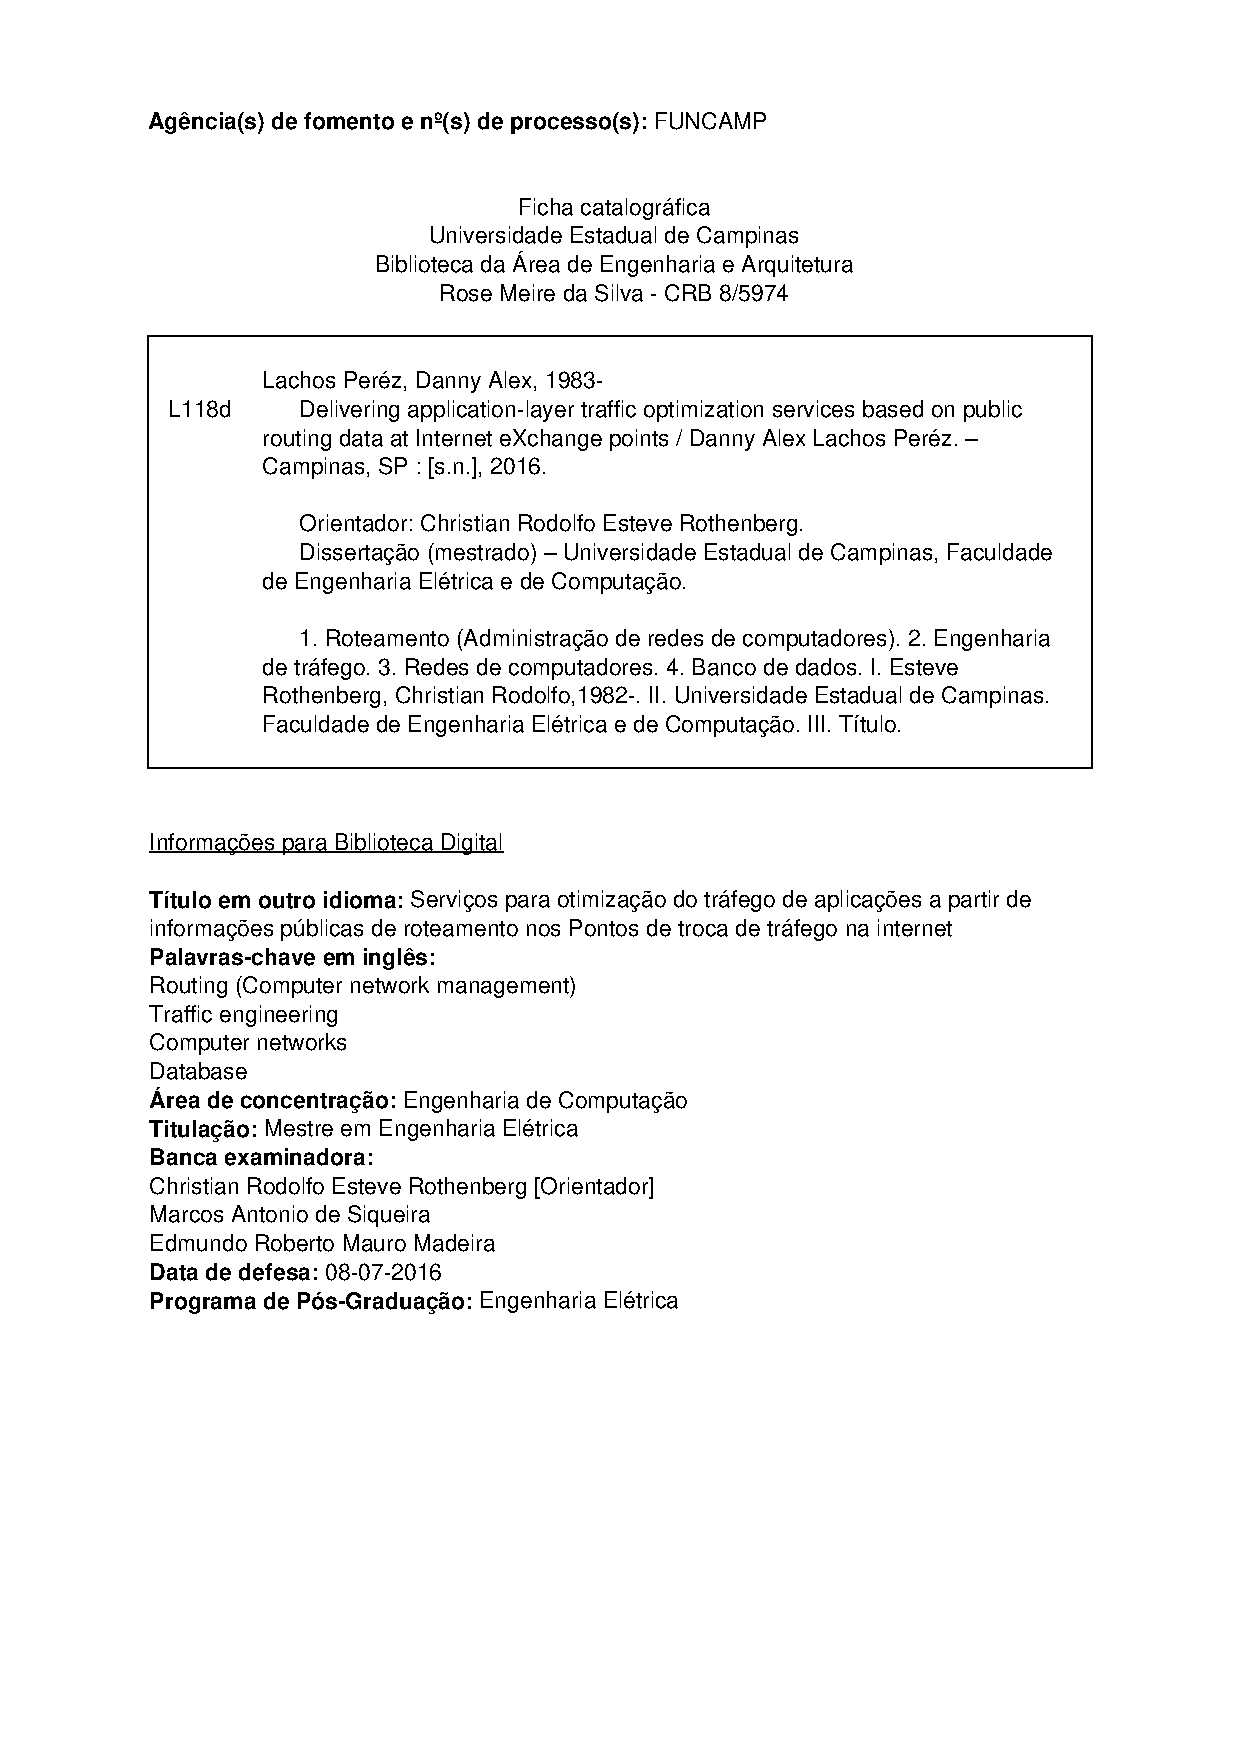
\includepdf[pages={1}]{docs/ficha-catalografica-protocolo.pdf}
%\includepdf{ficha-catalografica.pdf}
%% \end{fichacatalografica}
\newpage

% ---- ATA DA DEFESA----
%\vspace*{\fill}
%\begin{center}
%    \textsc{Inclua aqui a folha de assinaturas.}
%\end{center}
\AtaDeDefesa
%\vspace*{\fill}
\newpage
%\includepdf[pagecommand={\thispagestyle{plain}}]{folha-assinaturas.pdf}	
%\cleardoublepage

% ---- DEDICATÓRIA ----
\begin{dedicatoria}
\vspace*{\fill}
\centering
\noindent
\Dedicatoria
\vspace*{\fill}
\end{dedicatoria}

% ---- AGRADECIMENTOS ----
\begin{agradecimentos}
\Acknowledgements
\end{agradecimentos}

% ---- EPÍGRAFE ----
\begin{epigrafe}
\vspace*{\fill}
\begin{flushright}
\begin{minipage}{9.9cm}
\Epigrafe
\end{minipage}
\end{flushright}
\begin{flushright}
\textit{\EpigrafeAuthor}
\end{flushright}
\end{epigrafe}

% --- RESUMOS ---
\begin{resumo}
\Abstract
\newpage
\begin{otherlanguage*}{english}
\begin{center}{\ABNTEXchapterfont\huge Resumo}\end{center}
\Resumo
\end{otherlanguage*}
\end{resumo}

% ---- LISTA DE ILUSTRAÇÕES ----
\pdfbookmark[0]{\listfigurename}{lof}
\listoffigures*
\newpage
%\cleardoublepage

% ---- LISTA DE TABELAS ----
\pdfbookmark[0]{ \listtablename}{lot}
\listoftables*
\newpage
%\printglossary
%\cleardoublepage

% ----LISTA DE ACRONIMOS ----
%\printglossary[type=\acronymtype]
%\newpage
\clearpage
\printglossary[type=\acronymtype]
\printglossary
\newpage



% --- INSERIR SUMARIO ---
\pdfbookmark[0]{\contentsname}{toc}
\tableofcontents*
\cleardoublepage

% ---

%\input{acronyms}
%\renewcommand{\nomname}{Acronyms and Abbreviations List}
%%\pdfbookmark[0]{\nomname}{las}
%\printnomenclature
\cleardoublepage
% ---
\pagenumbering{arabic}
% \setcounter{page}{17}

% ---- ELEMENTOS TEXTUAIS ----
\textual

% ---- Introdu\c{c}\~{a}o ----
\interfootnotelinepenalty=10000
\sloppy
%%%%%%%%%%%%%%%%%%%%%%%%%%%%%%%%%%%%%%%%%%%%%%%%%%%%%%%%%%%%%%%%%%%%%%%%%%%%%%%%
\chapter{Introduction}\label{ch:introduction}
%%%%%%%%%%%%%%%%%%%%%%%%%%%%%%%%%%%%%%%%%%%%%%%%%%%%%%%%%%%%%%%%%%%%%%%%%%%%%%%

%4th-review
\section{Motivation}
 

The type of traffic used for performing evaluation matters; this is a fact. Studies show that realistic Ethernet traffic provides different and variable load characteristics on routers\cite{harpoon-validation}, even with the same average bandwidth consumption, showing that constant traffic is not sufficient for complete technology validation. This conclusion indicates that tests which employ traffic generators with constant rates are not enough for complete validation of new technologies. Bursty traffic can cause packet losses and buffer overflows, impacting network performance and measurement accuracy\cite{burstiness-queue-lenght}. Small packets tend to degrade application performance\cite{comparative-trafficgen-tools}.  Furthermore, realistic traffic is essential on security research, such as for the evaluation of firewall middleboxes, studies on intrusion, and malicious workloads\cite{ditg-paper}. 

New networking scenarios such as \acrshort{SDN} and virtualized networks (\acrshort{NFV} and \acrshort{VNF}s) become harder to predict in terms of performance compared to hardware-based technologies, due to the multiple layers of software and platform parameters demanding validation in a broadening range of use cases~\cite{nfv-challenges}. Another critical question about the interaction between application- network has had the flow-oriented operation of SDN networks, in which each new flow arriving on an SDN switch demands further communication with the controller. Therefore the controller can be a bottleneck on the switches performance.  Also,  new types of traffic patterns introduced by \acrshort{IoT} and Machine-to-Machine (\acrshort{M2M}) communication\cite{machine2machine}  increase the complexity of the network traffic characterization, turning pre-defined models used by traffic generators obsolete. 

Furthermore, realistic traffic generators are essential security research, since the generation of realistic workloads is essential for evaluation of firewall middleboxes. It includes studies of intrusion, anomaly detection, and malicious workloads. By realistic, we refer to traffic that represents well the traffic features, such as protocols, payloads, and protocols, able to emulate benign and malicious workloads. 

Aiming to address these gaps, this dissertation introduces \acrshort{SIMITAR}, an auto-configurable network traffic generator. SIMITAR stands for \textit{SnIffing, ModellIng, and TrAffic geneRation}, which correspond to the main operation processes of the proposed framework.  SIMITAR has an application independent traffic model, that can represent a wide variety of scenarios. It also decouples the traffic modeling and packet-generation layer, using a factory design pattern, enabling its application on different scenarios, and technology update, via technology abstraction.  SIMITAR code and all scripts used in this paper are available at GitHub\cite{projeto-github} for validation, experiment reproducibility, and re-use purposes. 


\section{Related Work}


\begin{table*}[ht!]
    \centering
    \caption{Comparison of existing traffic generation tools.}
    \scalebox{0.80}{ 
    \begin{tabular}{ccccc}
        \hline
        \rowcolor[HTML]{9B9B9B} 
        \hline
        \textbf{Solution}     & \textbf{Auto-configurable} & \textbf{Realistic Traffic} & \textbf{Traffic Custumization} & \textbf{Extensibility} \\ \hline
        Harpoon     & yes              & yes               & yes                   & \textbf{no}   \\
        \rowcolor[HTML]{C0C0C0} 
        D-ITG                & \textbf{no}      & yes               & yes                   & \textbf{no}   \\
        Swing                & yes              & yes               & \textbf{no}           & \textbf{no}   \\
        \rowcolor[HTML]{C0C0C0} 
        Ostinato             & \textbf{no}      & \textbf{no}       & yes                   & yes           \\
        LegoTG               & \textbf{no}      & \textbf{no}       & yes                   & yes           \\
        \rowcolor[HTML]{C0C0C0} 
        sourcesOnOff          & \textbf{no}      & yes               & yes                   & \textbf{no}   \\
        Iperf                & \textbf{no}      & \textbf{no}       & yes                   & \textbf{no}   \\ 
        \rowcolor[HTML]{C0C0C0} 
        SIMITAR          & yes      & yes               & yes                   & yes   \\ \hline
    \end{tabular}
    }
    \label{tab:related-work}
\end{table*}



Traffic generators are tools to transfer or inject network packets in a controlled manner,  aiming not at the actual data transfer data but at the functional validation and performance benchmarking of devices under test (\acrshort{DUT}) for varying technologies or scenarios. The open-source community offers a vast variety of traffic generators. Since most have been built for specific goals,  each uses different methods for traffic generation, and offer control over different traffic features, such as throughput, packet-sizes, protocols, and so on\cite{ditg-paper}. 

Traffic generators can be classified into two main groups: replay engines\cite{sourcesonoff-paper} and model-based tools. Replay engines, such as TCPReplay and TCPivo\cite{tcpivo-paper}, work replicating in a given network interface a given packet capture file. These tools can generate realistic traffic but have their constraints. They are deterministic since will always reproduce the same traffic from the packet capture. Replay engines require storage of packet capture, what can be a problem for traffics of high bandwidth traffic. Also, they assume the user has access to packet captures appropriate for his testing purposes, which is not always true, due to a limited number of public sources. Model-based tools rely on software models to replicate one or more characteristics of the traffic. 

%Following the taxonomy presented by Botta et al.\cite{do-you-trust}:
%\begin{itemize}
%\item \textbf{Application-level traffic generators}: they try to emulate network applications simulating real workloads stochastically and(or) responsively. Eg.: Surge, D-ITG\footnote{D-ITG works mainly on packet-level but can emulate some applications}.
%\item \textbf{Flow-level traffic generators}: they can reproduce features of flows, such as flow duration, a diurnal behavior. Eg.: Harpoon\cite{harpoon-validation}.
%\item \textbf{Packet-level traffic generators}: most traffic generators available fall in this class. They aim to reproduce physical features such as inter-packet times, packet size, bandwidth and packets per second. Eg.: Iperf\cite{web-iperf}, Ostinato\cite{web-ostinato}, D-ITG\cite{ditg-paper}, sourcesOnOff\cite{sourcesonoff-paper}.
%\item \textbf{Multi-level traffic generators}: it proposes to take into account existing interaction among each layer of the network stack. Eg.: Swing\cite{swing-paper}.
%\end{itemize}

Model-based tools have their limitations as well. Traffic generators that emulate the applications,  are designed to represent only specific scenarios on computer networking, and are not enough to represent a large variety of scenarios. Many  traffic generator tools only offer constant-rate and Poisson models, which does not represent well the complexity of internet traffic\cite{selfsimilar-ethernet}. Other tools such as D-ITG offer dozens of parameters and models to be configured, but delegate to the user the task of creating, validate and script his traffic model. To the best of our knowledge, we found only two open-source auto-configurable tools: Swing and Harpoon.  However, none of them has an extensible architecture, which turns supporting modern and fast \acrshort{I/O} \acrshort{API}s (such as DPDK\cite{web-dpdk}) a hard task. Table~\ref{tab:related-work} present a summary of the above mentioned features for some relevant traffic generators: Swing\cite{swing-paper}, Harpoon\cite{harpoon-validation}, sourcesOnOff\cite{sourcesonoff-paper}, D-ITG\cite{ditg-paper}, Iperf\cite{web-iperf}, Ostinato\cite{web-ostinato} and LegoTG\cite{legotg-paper}.


\section{Problem Statement}


Based on the provided context, we defined a set of targets for our research:


\begin{enumerate}

	\item \textbf{Research Topic I}:  Survey open-source Ethernet workload tools and address features each one has. We wanted to know the existing solutions, innovation points on the current state of affairs, and how can we some could be integrated and reused by our solution;
	
	\item \textbf{Research Topic II}: Study the characterization and mathematical modeling of Ethernet traffic, what are the best models and challenges. 
	
	\item \textbf{Research Topic III}: Define what realistic traffic generation is, and how to measure if any synthetic traffic is realistic or not. 
	
	\item \textbf{Design}: Create a general method for modeling and parameterization of Ethernet traffic;
	
	\item \textbf{Development}:  Create a self-configurable tool that observes and uses real network traffic, and reproduce its behavior characteristics, avoiding the storage of large pcap files. 
	
\end{enumerate}

Towards the above-stated objectives, we  had identified a set of requirements of the envisioned traffic generation tool should meet:

\begin{itemize}

\item \textbf{Auto-configurable}: It must be able to extract data from real traffic and store in a database, and use it to parametrize its traffic model. It must be able to obtain data from real-time traffics and from pcap files;

\item \textbf{Technology independent}: It must have a flow-based abstract model for traffic generation, not attached to any specific technology.

\item \textbf{Extensibility}: traffic modeling and generation must be decoupled. Ideally, it must be able to use as a traffic generator engine any library or traffic generator tool;

\item \textbf{Simple usage}: It must be easy to use. It has to take as input a Compact Trace Descriptor, just as a traffic replay engine (such as TCPreplay) would take a pcap file;

\item \textbf{ Human readable model}: it must produce a human-readable file as output that describes our traffic using our abstract model. We call this file a Compact Trace Descriptor(\acrshort{CDT});

\item \textbf{Traffic generation programmability}: It must have what we call traffic generation programmability. The compact trace descriptor must be simple and easy to read. That way, the user may want to create our custom traffic, in a platform agnostic way.

\item \textbf{Flow-oriented}: traffic modeling and generation must be flow-oriented. Each flow must be modeled and generated separately.

\end{itemize}


\begin{figure}[!ht]
    \centering
    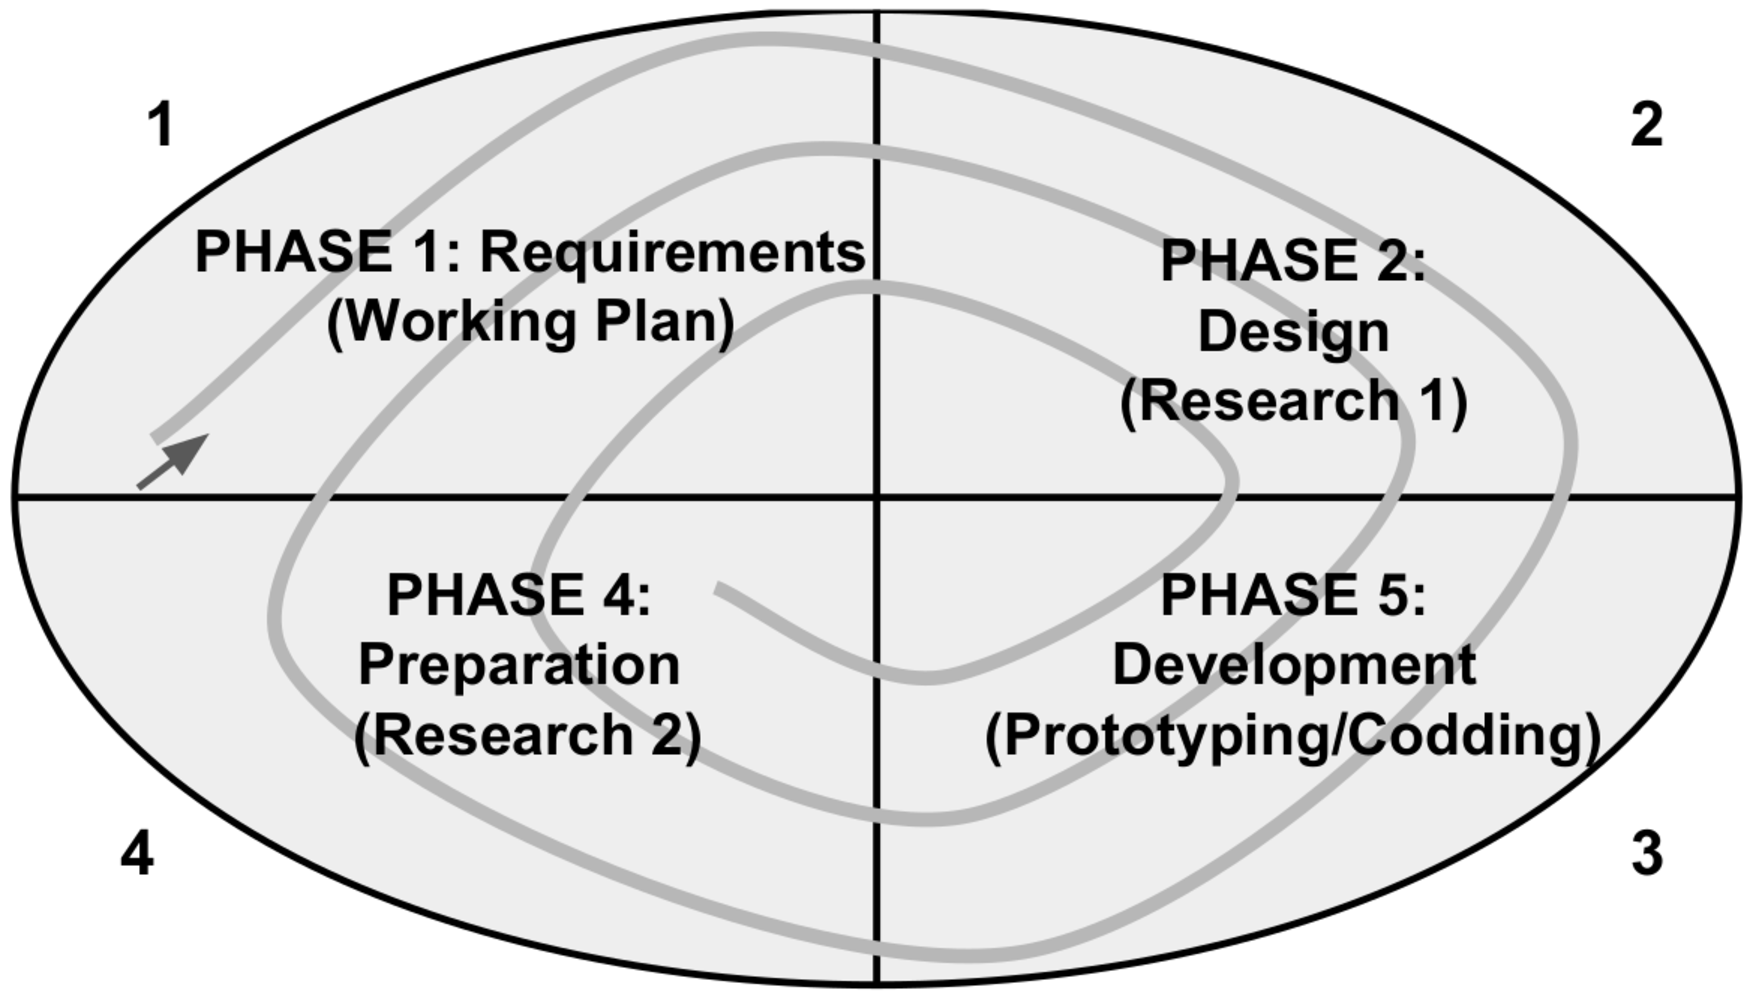
\includegraphics[scale=0.4]{figures/ch1/dev-cicle}
    \caption{Spiral research and development procedure}
    \label{fig:dev-cicle}
\end{figure}

We have adopted a spiral procedure of development, as suggested Sommerville on \textit{Software Engineering}\cite{sommerville}, but adapted to an academic research process. Figure ~\ref{fig:dev-cicle} shows the model of development we had adopted. It had four main phases: 

\begin{enumerate}
    \item \textit{Requirements (Working Plan)};
    \item \textit{Design (research 1)};
    \item \textit{Development (prototyping/codding)};
    \item \textit{Preparation (research 2)}.
\end{enumerate}

On the \textbf{Requirements phase}, we create tasks,  formalized on \textit{Working Plans} documents.  These tasks should cover the whole process. On the \textbf{Design (research 1) phase}, where the focus of the research are related works. We research on literature to learn about topics defined by the task, to help we design our solutions. On this step, during the initial phases of the project,  we also conceived the architecture along with \acrshort{UML} diagrams\footnote{Unified Modeling Language (UML) is a modeling language designed to provide a standardized way of representing and design systems\cite{uml}.}. Some small changes are inevitable, but structural changes turn to be impractical on later phases. The next phase is the \textbf{Development phase}. It is the prototyping and coding phase.  The last is the \textbf{Preparation phase} when we evaluate the results achieved on the Development phase, and we go back to research again,  aiming to prepare the next \textit{Working Plan}.  On this phase, the focus of the research is on points of innovation.


\section{Document Overview}


In this introductory chapter, we had presented an abstract of state of the art, and the main goals of our research. \textit{\textbf{Chapter~\ref{ch:literature-review}}} presents an extensive survey on open-source traffic generator tools, summarizing the benefits, and features supported by each one. The chapter offers a  review of topics on realistic traffic generation and defines important concepts on network traffic modeling; such as self-similarity and heavy-tailed distributions. Also, the chapter presents a survey on techniques for validating traffic generator tools 

\textit{\textbf{Chapter~\ref{ch:architecture}}} presents \textit{SIMITAR} traffic generator. We describe its low-level requirements and define an architecture and their algorithms.  We explain its operation and suggest some use cases. In \textit{\textbf{Chapter~\ref{ch:modeling-evaluation}}} we go deep on the modeling process we had developed for our traffic generator. We validate the effectiveness of Information Criteria \acrshort{AIC} and \acrshort{BIC} as a method selection of stochastic models for  Ethernet traffic.  We also discuss some other algorithms we developed such as \textit{calcOnOff} and the application protocol guesser. In \textit{\textbf{Chapter~\ref{ch:validation}}}, we define a set of metrics based on previous tests on validation of traffic generators found in the literature. Here, we focus on the packet, flow, and scaling metrics. We test our tool in an emulated SDN testbed with Mininet\cite{web-mininet}\footnote{Mininet is a network emulator. It can run a collection of  hosts, switches, routers and links over a single Linux kernel, using lightweight virtualization\cite{web-mininet-repo}.}, using OpenDayLight\cite{web-opendaylight} as a controller. 

\textit{\textbf{Chapter~\ref{ch:future-work}}}  highlights future actions to improve SIMITAR on realism and performance along with other future research avenues, including improving its computational performance, expand it to new APIs of traffic generation and calibration of its constants. Finally, we end the work presentation with a conclusion( \textit{\textbf{chapter~\ref{ch:conclusion}}}).
%%%%%%%%%%%%%%%%%%%%%%%%%%%%%%%%%%%%%%%%%%%%%%%%%%%%%%%%%%%%%%%%%%%%%%%%%%%%%%%%
\chapter{Literature Review}\label{ch:literature-review}
%%%%%%%%%%%%%%%%%%%%%%%%%%%%%%%%%%%%%%%%%%%%%%%%%%%%%%%%%%%%%%%%%%%%%%%%%%%%%%%%

%%%%%%%%%%%%%%%%%%%%%%%%%%%%%%%%%%%%%%%%%%%%%%%%%%%%%%%%%%%%%%%%%%%%%%%%%%%%%%%%
\section{Traffic Generators}\label{sec:traffic-gen}



Traffic generators are tools to transfer or inject network packets in a controlled manner,  aiming not at the actual data transfer data, but validation and performance benchmarking of devices under test (DUT)\cite{validate-trafficgen}. There is a vast variety of traffic generators described on literature \cite{ditg-paper} and available in the open-source community\footnote{\href{http://www.icir.org/models/trafficgenerators.html}{http://www.icir.org/models/trafficgenerators.html}}. 

Together with many traffic generators, there are many open-source APIs for traffic generation. Some are low-level APIs, which enables precise control of each packet generated, and are used in the implementation of traffic generators\footnote{For example: D-ITG\cite{ditg-paper} and Iperf\cite{web-iperf} uses the GNU Socket API\cite{web-socket}, Ostinato\cite{web-ostinato} uses libpcap\cite{web-libpcap}, and MoonGen\cite{moongen-paper} uses DPDK\cite{web-dpdk}. }. Also, they are computationally more efficient compared to high-level APIs for traffic generation. We've listed some low-level APIs below:

\begin{itemize}
\item GNU Socket API (C)\cite{web-socket};
\item Libpcap (C)\cite{web-libpcap};
\item Libtins (C++)\cite{web-libtins};
\item Scapy (Python)\cite{web-scrapy};
\item DPDK (C)\cite{web-dpdk}.
\end{itemize}

We also have high-level  APIs, usually provide by traffic generator, which simplifies the programming of custom traffic. For example:

\begin{itemize}
\item D-ITG API (C)\cite{web-ditg};
\item Ostinato API (Python)\cite{web-ostinato};
\item MoonGen API (Lua)\cite{web-moongen};
\item DPDK-Pktgen scripting interface (Lua)\cite{web-dpdk-pktgen}.
\end{itemize}

There are many taxonomies for traffic generators available on the literature. Classify traffic generators is usually "blur" process since packet generators feature many times fall in more than one class. We present two  taxonomies: 

\begin{itemize}
\item Traffic generation strategy;
\item Traffic generator implementation.
\end{itemize}

%%%%%%%%%%%%%%%%%%%%%%%%%%%%%%%%%%%%%%%%%%%%%%%%%%%%%%%%%%%%%%%%%%%%%%%%%%%%%%%
\subsection{Traffic generators by strategy}


Traffic generators can be classified into two main groups: replay engines\cite{sourcesonoff-paper} and model-based tools:

\begin{itemize}
\item \textbf{Replay engines}: These tools can read pcap files, and inject copies of the packet on a network interface. Eg.: TCPReplay\cite{web-tcpreplay}, TCPivo\cite{tcpivo-paper}, D-ITG\cite{ditg-paper}.
\item \textbf{Model-based traffic generators}: they generate synthetic traffic, controlling one or more feature of the traffic; such as header fields, packet sizes and inter-packet times.  
\end{itemize}

Model-based traffic generators can be sub-classified based on the abstraction layer the model operates. We follow here the taxonomy presented by Botta et al.\cite{do-you-trust}. Figure~\ref{fig:layers-workload-tools} shows these traffic generators organized in a layer diagram.

\begin{itemize}

\item \textbf{Application-level traffic generators}: they try to emulate the behavior of network applications, simulating real workloads stochastically or responsively 3. As an example, we have Surge, which emulates the communication between clients and web
servers;

\item \textbf{Flow-level traffic generators}: they can reproduce flow characteristics, such as flow duration, start times distributions, and temporal diurnal traffic volumes. Harpoon can extract these parameters from Cisco NetFlow data, collected from routers;

\item \textbf{Packet-level traffic generators}: it is the most used traffic generators. They can control packet-features like inter-departure times, packet size, throughput and packets per second. For example, D-ITG\cite{ditg-paper}, and TG\cite{web-tg} can control inter-packet times via stochastic distributions. However, most of them only permit the configuration of constant-rate models, by setting the packet rate or the traffic bandwidth, such as Iperf\cite{web-iperf}, BRUNO\cite{bruno-paper} and Ostinato\cite{web-ostinato}.

\item \textbf{Multi-level traffic generators}: this is a more recent class of network traffic generator. They take into account existing interaction among each layer of the network stack, to create network traffic as close as possible to reality. The most relevant tool is Swing\cite{swing-paper} which input collected pcap files. 

\end{itemize}


We have done an extensive survey on packet generators available on the open-source community, and classified them according to the first taxonomy. Also, we summarized the main features of each one. The result of this work is the tables \label{tab:app-level-tg}, \label{tab:multi-level-tg}, \label{tab:packet-level-tg}, and \label{tab:replay-tg}, in the appendix ~\ref{ap:traffic-gen-survey}. We also have a list of the tool repositories at table~\ref{tab:traffic-gen-links}


%%%%%%%%%%%%%%%%%%%%%%%%%%%%%%%%%%%%%%%%%%%%%%%%%%%%%%%%%%%%%%%%%%%%%%%%%%%%%%%
\subsection{According to the implementation of traffic generators}

\begin{itemize}

\item \textbf{Software-only traffic generators}: Implementations of traffic generators utterly independent of its running hardware platform. This implementation comprehends most of traffic generator tools, including all previously mentioned. 

\item \textbf{Software and hardware-dependent traffic generators}: are traffic generators implemented in software, but dependent on the underlying hardware. The most preeminent examples of this class used DPDK\cite{web-dpdk} as packet-generator API. DPDK works directly on the \acrshort{NIC} interface, avoiding overheads of the Operational System. As cited on its official website, this approach permits huge precision. As examples we have MoonGen\cite{moongen-paper} and DPDK-PktGen\cite{web-dpdk-pktgen}

\item \textbf{Hardware traffic generators}: these open-source traffic generators are implemented in hardware description language (VHDL/Verilog), and work on \acrshort{NetFPGA}s. Some examples of implementations are PacketGenerator\cite{pktgen-netfpga-paper}, Caliper\cite{caliper-paper}, and OSNT Packet Generator\cite{osnt-paper}.

\end{itemize}


\begin{figure}[!ht]
	\centering
	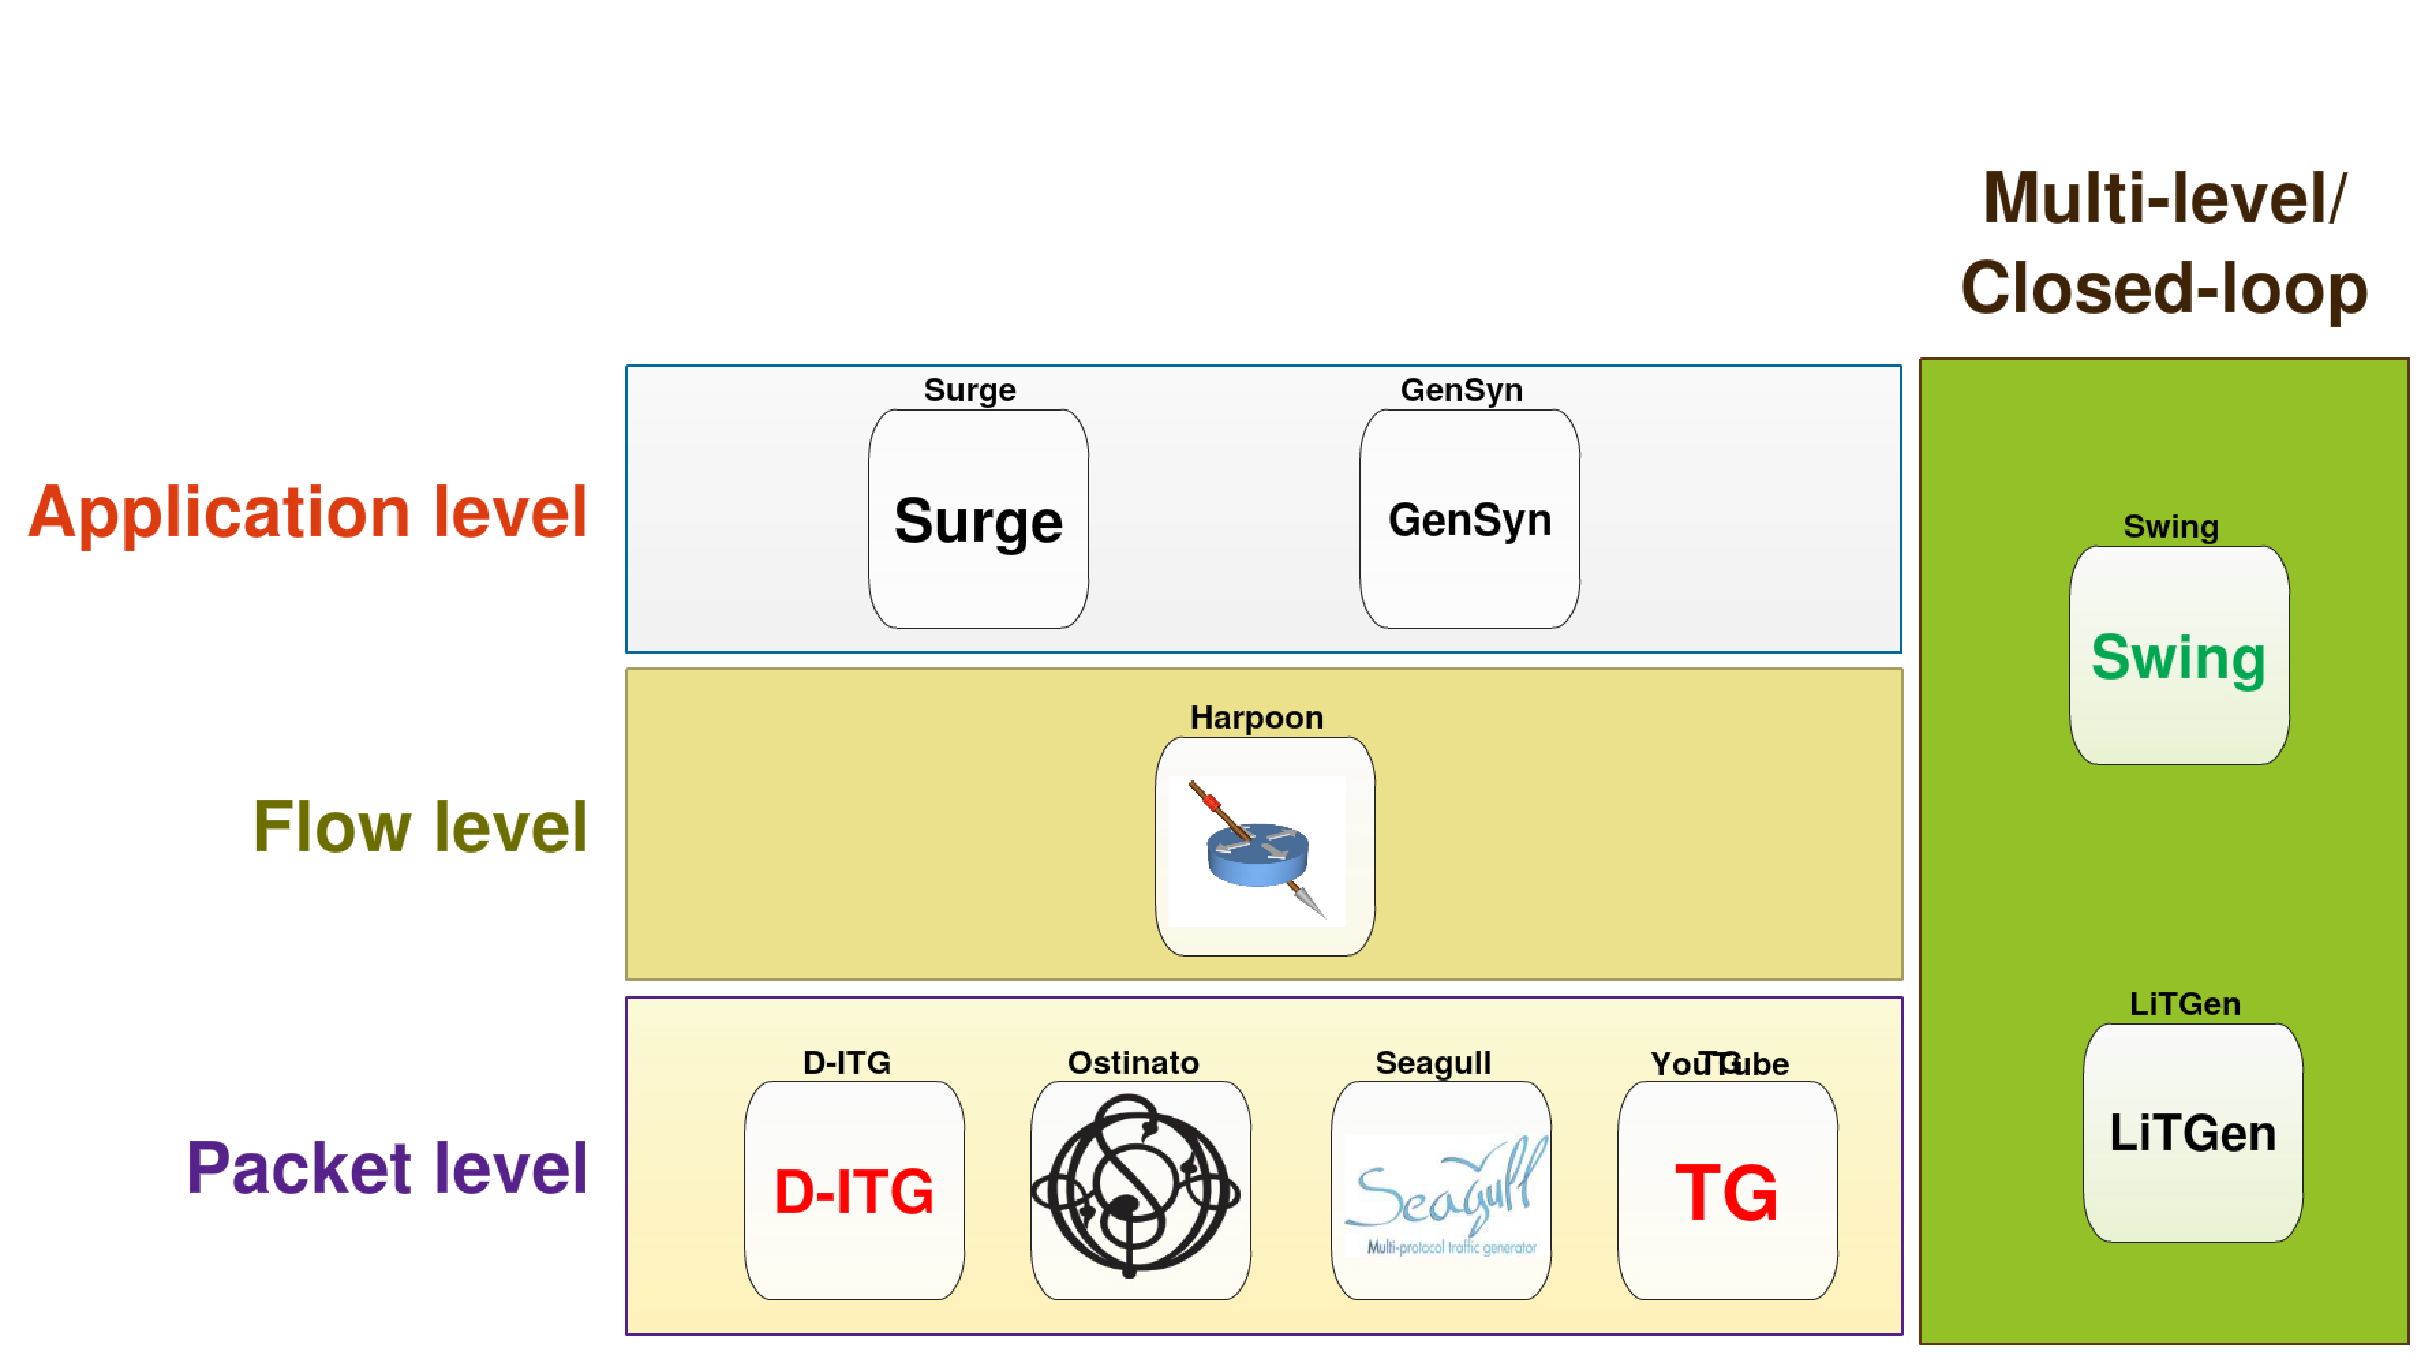
\includegraphics[scale=0.4]{figures/ch2/types-workload-tools}
	\caption{Diagram representing different traffic generators, according to its abstraction layer.}
	\label{fig:layers-workload-tools}
\end{figure}





%%%%%%%%%%%%%%%%%%%%%%%%%%%%%%%%%%%%%%%%%%%%%%%%%%%%%%%%%%%%%%%%%%%%%%%%%%%%%%%
\section{Realistic Traffic and Traffic Modeling}\label{sec:modeling-traffic}

\subsection{Realistic Network Traffic Generation}

As presented, there is a considerable amount of open-source traffic generators available, each one of them with many different sets of features available. However, on the generation of realistic workload, the set of possibilities become much more restricted. On the other hand, there are many works on characterization, modeling, and simulation of different types of network workload. As stated by Botta et al., a synthetic network traffic generation over real networks should be able to: 

\begin{enumerate}
\item Capture real traces complexity over different scenarios;
\item Be able to custom change some specific properties of the generated traffic ;
\item Return measure indicators of performance experienced by the workload.
\end{enumerate}


As we have found out over the literature in our research, the measure of realism of a traffic generator is given by how well a traffic generator can represent features at the level its model works. For example:

\begin{itemize}
\item \textbf{Swing}: Vishwanath and Vahdat\cite{swing-paper} validate their work against packet, flow, and application level features;
\item \textbf{Harpoon}: Sommers and Barford\cite{harpoon-validation} validate harpoon on flow-level features;
\item \textbf{D-ITG}: Botta et al.\cite{ditg-paper} validate their work against application-level and packet-level features;
\item \textbf{sourcesOnOff}: Varet and Larrieu validate sourcesOnOff on packet-level features\cite{sourcesonoff-paper}. 
\end{itemize}

Therefore, we defined a realistic traffic generator as follows:

\vspace{5mm}
\begin{tcolorbox}[colback=blue!5,colframe=blue!40!black,title=Realistic Traffic Generator]
A realistic traffic generator is a tool that its model can reproduce real traces complexity and behavior, at the same level of abstraction its traffic model works: on the packet, flow, application or multi-level. In other words, the validation techniques must give similar results to the real and synthetic traces. 
\end{tcolorbox}
\vspace{5mm}

We are going to discuss metrics on validation of traffic generators in the next section. The rest of this section will highlight topics on network traffic modeling. We are not going to discuss application modeling, since each one may have their specific behavior. We are going to discuss points that apply to any traffic in general:

\begin{itemize}
\item Inter-packet times (throughput) modeling;
\item Packet-sizes modeling;
\item Packet-header fields;
\item Flow modeling;
\item Closed-loop behavior modeling.
\end{itemize}

%%%%%%%%%%%%%%%%%%%%%%%%%%%%%%%%%%%%%%%%%%%%%%%%%%%%%%%%%%%%%%%%%%%%%%%%%%%%%%%
\subsection{Inter-packet times (throughput) modeling}


\begin{table}[t!]
\centering
\caption{Probability density function (\acrshort{PDF}) and Cumulative distribution function (\acrshort{CDF}) of some random variables, and if this stochastic distribution has or not self-similarity property. Some functions used to express these distributions are defined at the table ~\ref{tab:distributions-definitions} }
\label{tab:distributions-equations}
\scalebox{0.82}{ 
\begin{tabular}{lcccr}
Distribution & PDF Equation & CDF Equation & Parameters & Heavy-tailed\\ \hline
\\
\multirow{2}{*}{Poisson} & \multirow{2}{*}{$f[k] = \frac{e^{-\lambda}\lambda^k}{k!}$} & \multirow{2}{*}{$F[k] = \frac{\Gamma(\lfloor k + 1 \rfloor, \lambda)}{ \lfloor k \rfloor!}$} &  $\lambda > 0$  (mean, \\
 &  &  & variance) & no \\ 
\\ 
\multirow{2}{*}{Binomial} & \multirow{2}{*}{$f[k] = \binom{n}{k}p^{k}(1 - p)^{n - k} $} & \multirow{2}{*}{$F[k] = I_{1 - p}(n - k, 1 + k)$} &  $n > 0$ (trials)\\  &  &  &$p > 0$ (success)  & no \\ 
\\
\multirow{2}{*}{Normal} & \multirow{2}{*}{$f(t) =  \frac{1}{\sqrt[]{2\sigma^2}\pi}e^{\frac{(t - \mu)^2}{2\sigma^2}}$ } & \multirow{2}{*}{ $F(t) = \frac{1}{2}[ 1 + \text{erf}(\frac{t - \mu}{\sigma\sqrt[]{2}})]$ } &  $\mu$ (mean) \\ &  &  & $\sigma > 0$ (std.dev) & no \\ 
\\ 
\multirow{2}{*}{Exponential} & \multirow{2}{*}{ $f(t) = \begin{cases} \lambda e^{-\lambda t} ;& t \geq 0 \\ 0;& t < 0 \end{cases} $  }   & \multirow{2}{*}{ $F(t) = 1 - e^{-\lambda t} $ } & \\ &  &  & $\lambda > 0$ (rate)  & no \\ 
\\
\multirow{2}{*}{Pareto} & \multirow{2}{*}{$f(t) = \begin{cases} \frac{\alpha t_{m}^\alpha}{t^{\alpha + 1}} ;& t \geq t_{m} \\ 0;& t < t_{m} \end{cases} $ } & \multirow{2}{*}{$F(t) = \begin{cases} 1 - (\frac{t_{m}}{t})^\alpha ;& t \geq t_{m} \\ 0;& t < t_{m}\end{cases} $} &  $\alpha > 0$ (shape)  \\ & &  &  $t_{m} > 0$ (scale)   & yes \\ 
\\ 
\multirow{2}{*}{Cauchy} & \multirow{2}{*}{ $f(t) = \frac{1}{\pi \gamma}[\frac{\gamma^2}{(t - t_{0})^{2} + \gamma^{2}}]$ } & \multirow{2}{*}{ $F(t) = \frac{1}{\pi}\arctan( \frac{t - t_{0}}{\gamma} ) + \frac{1}{2}  $ } &  $\gamma > 0$ (scale) \\ &  &   & $t_{0} > 0$ (location) & yes \\  
\\
\multirow{2}{*}{Weibull} & \multirow{2}{*}{ $f(t) = \begin{cases} \frac{\alpha}{\beta^\alpha}t^{\alpha - 1}e^{(t/\beta)^{\alpha}}; & t \geq 0 \\ 0; & t < 0 \end{cases}$  } & \multirow{2}{*}{ $F(t) = \begin{cases} 1 - e^{-(t/\beta)^{\alpha}}; & t \geq 0 \\ 0 ; & t < 0  \end{cases}$ } & $\alpha  > 0 $ (shape) \\ &  &  & $\beta > 0$ (scale)  & yes \\
\\
\multirow{2}{*}{Gamma} & \multirow{2}{*}{ $ f(t) = \frac{\beta^{\alpha}}{\Gamma(\alpha)}t^{\alpha - 1}e^{-\beta t}  $ } & \multirow{2}{*}{$ F(t) = 1 - \frac{1}{\Gamma(\alpha)}\Gamma(\alpha, \beta x) $} & $\alpha > 0$ (shape) \\ &  &  & $\beta > 0$ (rate) & no \\
\\ 
%\multirow{2}{*}{Student's t} & \multirow{2}{*}{} & \multirow{2}{*}{} &  \\ &  &  & & \\ 
%\\
\multirow{2}{*}{Beta} & \multirow{2}{*}{ $ f(t) = \frac{x^{\alpha - 1}(1 - x)^{\beta - 1}}{B(\alpha, \beta)} $ } & \multirow{2}{*}{ $ F(t) = I_{x}(\alpha, \beta) $ } &  $\alpha > 0$ (shape) \\ &  &  & $\beta > 0$ (shape) & no \\ 
\\ 
\multirow{2}{*}{Log-normal} & \multirow{2}{*}{ $ f(t) = \frac{1}{t \sigma \sqrt[]{2 \pi}}e^{- \frac{(\ln(x) - \mu)^{2}}{2 \sigma^{2}}} $ } & \multirow{2}{*}{ $ F(t) = \frac{1}{2} + \frac{1}{2}\text{erf}[\frac{\ln(x) - \mu}{\sqrt[]{2} \sigma}] $ } & $\mu$ (location)\\
 &  &  & $ \sigma > 0 $ (shape) & yes \\ 
\\
\multirow{2}{*}{Chi-squared} & \multirow{2}{*}{ $ f(t) = \frac{1}{2^{\frac{k}{2}}\Gamma(\frac{k}{2}) }t^{\frac{k}{2} - 1}e^{-\frac{t}{2}} $ } & \multirow{2}{*}{ $ F(t) = \frac{1}{\Gamma(\frac{k}{2})}\gamma(\frac{k}{2}, \frac{x}{2}) $ } &  \\
 &  &  & $ k \in \mathbb{N}_{>0} $ &  no\\ 
\\
 
\hline
\end{tabular} 
} %scalebox
\end{table}

\begin{table}[t!]
\centering
\caption{Definitions of some functions used by PDFs and CDFs}
\label{tab:distributions-definitions}
\begin{tabular}{ll}
\hline
Function                             & Definition \\ 
\hline
\\
Regularized Incomplete beta function & $ I_{x}(a, b) = \frac{B(x| a, b)}{B(a, b)} $           \\
\\
Incomplete beta function             & $ B(x| a, b) = \int_{0}^{x} t^{a - 1} (1 - t)^{(b - 1)} \text{d}t $           \\
\\
Beta function                        & $ B(x| a, b) = \int_{0}^{1} t^{a - 1} (1 - t)^{(b - 1)} \text{d}t $           \\
\\
Error function                       & $ \text{erf}(x) = \frac{1}{\sqrt[]{\pi}}\int_{x}^{-x} e^{-t^{2}} \text{d}t $           \\ 
\\
Lower incomplete Gamma function      & $ \gamma(s, x) = x^{s}\Gamma(s)e^{-x}\sum_{k = 0}^{\infty}\frac{x^{k}}{\Gamma(s+k+1)} $  \\
\\
\hline
\end{tabular}
\end{table}


Classical models for network traffic generation were the same used in telephone traffic, such as  Poisson or Poisson-related, like Markov and Poisson-batch. They can describe the randomness of an Ethernet link but cannot capture the presence of "burstiness" in a long-term time scale, such as traffic "spikes" on long-range "ripples". Lerand et al.\cite{selfsimilar-ethernet}, points in his seminal work, in 1994, that the nature of the Ethernet traffic is self-similar. It has a fractal-like shape since characteristics seen in a small time scale should appear on a long-scale as well, that have been referred, in the most of the time, as long-range dependence or degree of long-range dependence (LRD). One way to identify if a process is self-similar is by checking its Hurst parameter, or Hurst exponent H, as a measure of the "burstiness" and LRD.  A random process is self-similar and LRD if $0.5 < H <1$\cite{stochastic-selfsimilar}. 

Willinger et al. pointed out that the Ethernet traffic has a high variability (or infinite variance)\cite{selfsimilar-highvariability}.  Processes with such characteristic are said to be heavy-tailed. In practical terms, that means a sudden discontinuous change can always occur. Heavy tail shows that a stochastic distribution is not exponentially bounded. In other words, some value far from the mean does not have a negligible probability of occurrence. We can express self-similar and heavy-tailed processes using heavy-tailed stochastic distributions, such as Pareto and Weibull. Table~\ref{tab:distributions-equations} shows the reference for these stochastic distributions. In the last column, we indicate if the distribution is or not heavy-tailed. 

These concepts of  High variability and Self-similarity are called Noah and Joseph Effects\cite{selfsimilar-highvariability}. Willinger et al. point that the superposition of many ON/OFF sources (or packet trains) using ON and OFF times that obey the Noah Effect (heavy-tailed probabilistic functions), also obey the Joseph effect. That means, it is a self-similar process and can be used to describe Ethernet traffic. Some works on the literature on synthetic traffic uses this principle, like sourcesOnOff\cite{sourcesonoff-paper}, or have to heavy-tailed processes, such as like D-ITG.

Furthermore, some later studies advocate the use of more advanced multiscaling models (multifractal), addressed by investigations that uses envelope processes\cite{envelope-process}. 


%%%%%%%%%%%%%%%%%%%%%%%%%%%%%%%%%%%%%%%%%%%%%%%%%%%%%%%%%%%%%%%%%%%%%%%%%%%%%%%
\subsection{Packet-sizes modeling}


\begin{table}[t!]
\centering
\caption{Two different studies evaluating the impact of packet size on the throughput. Both compare many available open-source tools on different testbeds. In all cases, small packet sizes penalize the throughput. Bigger packet sizes achieve a higher throughput.}
\label{tab:packet-size-impact}
\scalebox{0.9}{
\begin{tabular}{|l|c|c|c|}
\hline
 & \multicolumn{3}{c|}{Traffic Generators} \\ \cline{2-4} 
\multicolumn{1}{|c|}{Article and setup} &  & \multicolumn{1}{c|}{Maximum bit-rate} & \multicolumn{1}{c|}{Maximum bit-rate} \\
 & \multicolumn{1}{c|}{Toll} & \multicolumn{1}{c|}{\begin{tabular}[c]{@{}c@{}}at small packet \\ sizes\end{tabular}} & \multicolumn{1}{c|}{\begin{tabular}[c]{@{}c@{}}at big packet \\ sizes\end{tabular}} \\ \hline
\textit{\begin{tabular}[c]{@{}l@{}}Comparative study of various \\ Traffic Generator Tools \cite{comparative-trafficgen-tools} ;\end{tabular}} & PackETH & 150 @(64 bytes) & 1745 @(1408 bytes) \\ \cline{2-4} 
\begin{tabular}[c]{@{}l@{}}setup: Linux (Centos 6.2, \\ Kernel version 2.6.32),\end{tabular} & Ostinato & 135 @(64 bytes) & 2850 @(1408 bytes) \\ \cline{2-4} 
\begin{tabular}[c]{@{}l@{}}Inter(R) Xeon(R) CPU with 2.96GHz,\\  RAM of 64GB , NIC Mellanox\end{tabular} & D-ITG & 62 @(64 bytes) & 1950 @(1408 bytes), \\
\begin{tabular}[c]{@{}l@{}}Technologies MT25418 {[}ConnectXVPI \\ PCIe 2.0 2.5GT/s - IB DDR{]}\end{tabular} &  &  & \begin{tabular}[c]{@{}l@{}}9808 @(1460 bytes, \\ 12 threads)\end{tabular} \\ \cline{2-4} 
10 Bbps. Protocol: TCP & Iperf & * & \begin{tabular}[c]{@{}l@{}}8450 @(1460 bytes, \\ 12 threads)\end{tabular} \\ \hline
\textit{\begin{tabular}[c]{@{}l@{}}Performance Monitoring of Various \\ Network Traffic Generators \cite{performance-trafficgen};\end{tabular}} & Iperf & 46.0 @(128 bytes) & 93.1 @(1408 bytes) \\ \cline{2-4} 
\begin{tabular}[c]{@{}l@{}}Inter(R) Pentium 4(R), CPU \\ with 3.0GHz, RAM 1GB,\end{tabular} & Netperf & 46.0 @(128 bytes) & 89.9 @(1408 bytes) \\ \cline{2-4} 
\begin{tabular}[c]{@{}l@{}}NIC Intel Pro/100 Adapter \\ (100Mbps),\end{tabular} & D-ITG & 38.1 @(128 bytes) & 83.1 @(1408 bytes) \\ \cline{2-4} 
\begin{tabular}[c]{@{}l@{}}Hard Drivers Seagate Barracuda \\ 7200 series with 20BG. \\ Protocol:TCP\end{tabular} & IP Traffic & 61.0 @(128 bytes) & 76.7 @(1408 bytes) \\ \hline
\end{tabular}
}
\end{table}

The literature shows that the packet size of a trace may result in a considerable impact in a trace throughput since small packets cause a significant overhead on packet processing\cite{stochastic-selfsimilar}\cite{performance-trafficgen}. Table~\ref{tab:packet-size-impact} summarizes the results from two different works about throughput impact of packet sizes. On packet size distributions’ characterization, we can find many works as well.  For example, Castro et al. pointed that  90\% of \acrshort{UDP} packets were smaller than 500 bytes, and most packets transmitted using \acrshort{TCP} have 40 bytes (acknowledgment) and 1500 bytes (Maximum Transmission Unit, MTU)\cite{packet-distribution-model}. Ostrowsky et al.  found that on UDP traces, the modes of two regions were 120 and 1350 bytes, with a cut-off value of 750 bytes. They also found that roughly UDP packets constituted 20\% of the total number of packets on captures\cite{udp-flows-model}. Castro et al. points on his work that capture traces made on routers were all bimodal, and the majority is TCP. However, the size of each mode may change depending on the application. For example, an \acrshort{HTTP} traffic tends to have a mode closer to the \acrshort{MTU} compared to an \acrshort{FTP} capture\cite{packet-distribution-model}.


%%%%%%%%%%%%%%%%%%%%%%%%%%%%%%%%%%%%%%%%%%%%%%%%%%%%%%%%%%%%%%%%%%%%%%%%%%%%%%%
\subsection{Packet-header fields}

Accurate replication of network traffic should be able to control packet headers such as protocols, ports, addresses, and so on. Traffic generators provide support for these features, more frequently in a limited way. Most offer support just common protocols, such as TCP, UDP, and \acrshort{IPv4}. On the other hands, there are some which provide a vast variety of support and control over packet headers like PackETH\cite{web-packeth} and D-ITG\cite{web-ditg}. Other tools are even able to enable someone to extend this feature and develop support to new protocols. For example, Ostinato and Seagull permit the customization and creation of protocols\cite{wp-seagull}.


%%%%%%%%%%%%%%%%%%%%%%%%%%%%%%%%%%%%%%%%%%%%%%%%%%%%%%%%%%%%%%%%%%%%%%%%%%%%%%%
\subsection{Flow modeling}

Some packet-level traffic generators permit the control of flow generation, mostly manually through an API or scripting. In terms of automatic flow configuration, an example is Harpoon\cite{harpoon-paper}, which can to automatically configure its flows, using as input NetFlow Cisco traffic traces to automatically setting parameters. Harpoon deals with flow modeling in three different levels: file level, session level, and user level, not dealing with packet level at all. In the file level, Harpoon model two parameters: the files size and the time interval between consecutive file requests, called inter-file request time. The middle level is the session level, that consist of sequences files transfer between two distinct \acrshort{IP} addresses. The session level has three components: the IP spatial distribution, the second is the inter-session start times and the third is the session duration. The last level is the user level. In Harpoon, "users" are divided on "TCP" and "UDP" users, which conduct consecutive session using these protocols. This level has two components: the user ON time, and the number of active users. By modeling the number of users, Harpoon can reproduce temporal (diurnal) traffic volumes.


%%%%%%%%%%%%%%%%%%%%%%%%%%%%%%%%%%%%%%%%%%%%%%%%%%%%%%%%%%%%%%%%%%%%%%%%%%%%%%%
\subsection{Closed-loop(responsive) models}

The closed-loop operation means that the traffic generator uses feedback to reconfigure its model. That means the traffic generator can change its behavior at run time according to the observation made in real-time, changing the traffic created. These modifications involve changes on parameters of statistical distributions of inter-departure time and packet size, for example. Swing\cite{swing-paper} and application-level traffic generators like Surge\cite{surge-paper} and GenSyn\cite{gensyn-paper}uses this strategy.





%%%%%%%%%%%%%%%%%%%%%%%%%%%%%%%%%%%%%%%%%%%%%%%%%%%%%%%%%%%%%%%%%%%%%%%%%%%%%%%%
\section{Validation of Traffic Generator Tools}~\label{sec:validation-traffic-gen}


After the implementation of a traffic generator, it needs to be validated. Thus, we need a set of proof of concepts to evaluate if it reached its purposes or not. Researchers have been proposed many validation techniques, according to the traffic generator intended behavior. Magyesi and Szabó\cite{validate-trafficgen} presented a survey of these techniques, grouped by type of metric. The authors classified the techniques into four categories: packet based metrics, flow-based metrics, scaling characteristics, and \acrshort{QoS}/\acrshort{QoE} related metrics. Here we present a short review of each group of these validation techniques.


%%%%%%%%%%%%%%%%%%%%%%%%%%%%%%%%%%%%%%%%%%%%%%%%%%%%%%%%%%%%%%%%%%%%%%%%%%%%%%%%
\subsection{Packet Based Metrics}

Packet-based metrics are the most used metrics in the validation of traffic generators\cite{validate-trafficgen}. The most relevant packet based metrics are throughput\cite{do-you-trust}\cite{comparative-trafficgen-tools}\cite{performance-trafficgen}\cite{moongen-paper} (bytes and packets), packet size distribution\cite{packet-distribution-model} and inter-packet time distribution (inter-arrival and inter-departure)\cite{sourcesonoff-paper} \cite{ditg-paper}.


%%%%%%%%%%%%%%%%%%%%%%%%%%%%%%%%%%%%%%%%%%%%%%%%%%%%%%%%%%%%%%%%%%%%%%%%%%%%%%%%
\subsection{Flow Based Metrics}


Flow-based metrics are becoming more critical since newer network elements, like SDN devices, can execute flow-based operations\cite{validate-trafficgen}\cite{sdn-survey}. Magyesi and Szabó\cite{validate-trafficgen} consider the essential flow metrics, the flow size distribution, and volume. The flow volume stands for the number of flows of traffic. The flow size distribution is a measure of the length on time from the flows in network traffic. The flow volume is proportional to the number of flow instances that a flow-based device should run simultaneously. Moreover, the flow sizes define how much time each of these instances will run.


%%%%%%%%%%%%%%%%%%%%%%%%%%%%%%%%%%%%%%%%%%%%%%%%%%%%%%%%%%%%%%%%%%%%%%%%%%%%%%%%
\subsection{Fractal and Scaling Characteristics}

Second order characteristics such as "burstiness" and long-range dependence are responsible for the complex nature of internet traffic\cite{validate-trafficgen}. Due to its non-stationary nature, traditional methods fail to extract useful information\cite{validate-trafficgen}. The first analysis made in that way focused on the estimation of the Hurst exponent\cite{selfsimilar-ethernet}. They demonstrated the self-similar nature of the Ethernet traffic. As explained before, self-similar traffic should be in a Hurst exponent $H$, such as $0.5 < H < 1$. Over the years, wavelet-based analysis has become an efficient way to reveal correlations, bursts and scaling nature of the Ethernet traffic\cite{validate-trafficgen}. Many papers have used wavelet-based analysiscite{swing-paper}\cite{non-intrusive-wavelet}\cite{wavelet-analysis-long-range}. Huang et al.\cite{non-intrusive-wavelet} and Abry and Veitch\cite{wavelet-analysis-long-range} offer an extensible explanation of wavelet-based scaling analysis (\acrshort{WSA}) or wavelet multi-resolution energy analysis (\acrshort{WMA}). The explanation about the primary information offered by these two works will be showed below. 

First, consider a time series $X_{0,k}$ for $k = 0, 1, ... 2^n$:

\begin{equation}
\{X_{0,k}\} = \{ X_{0,0}, X_{0,1}, ... ,X_{0,2^{n}} \}
\end{equation} 

Suppose that we coarser $X_{0}$ in another time-series $X_{1}$ with half of the original resolution, but using  $ \sqrt[]{2} $ as normalization factor:

\begin{equation}
X_{1,k} = \frac{1}{\sqrt{2}}(X_{0,2k} + X_{0,2k+1})
\end{equation}

If we take the differences, instead of the averages, evaluate the so-called \textit{details}.

\begin{equation}
d_{1,k} = \frac{1}{\sqrt{2}}(X_{0,2k} - X_{0,2k+1})
\end{equation}

We can continue repeating this process, writing more coarse time series $X_{2}$ from $X_{1}$, until we reach $X_{n}$. Therefore, we will get a collection of \textit{details}:

\begin{equation}
\{d_{j,k}\} = \{ d_{1,0}, d_{1,1}, ..., d_{1,2^{n/2}}, ..., d_{n, 0} \}
\end{equation}

This collection of details ${d_{j,k}}$ are called Discrete Haar Wavelet Transform. Using the \textit{details}, we can calculate the energy function $E_{j}$, for each scale $j$, using:

\begin{equation}
E_{j} = \frac{1}{N_{j}} \sum_{k = 0}^{N_{j} - 1} |d_{j,k}|^{2}; \qquad j = 1, 2, ..., n
\end{equation} 
\\ 
were $N_{j}$ is the total number of coefficients at scale $j$. If we plot $\log(E_{j})$ as a function o the scale $j$, we will obtain a wavelet multiresolution energy plot.

On energy wavelet multiresolution energy plots, it is possible to capture three different central behavior, according to the scale. On \textbf{periodic time series}, the Energy values will be small. In fact, on perfectly periodic scales $j$, the values of the energy function $E_{j}$ will be zero. So periodicity will be sensed if the value of the energy function decrease. Perfect \textbf{white noise time series} will maintain the same value of the energy function. So an approximately constant value for the energy function $E_{j}$ indicates white noise behavior (which can be represented by a Poisson process\cite{poisson-white-noise}). On \textbf{self-similar time series}, the energy function plot $\log(E_{j})$ grows approximately linearly with the scale $j$. This characteristic explains why it has become a standard for realistic traffic generation analysis. In a single plot, we can quickly identify periodicities, and self-similar and Poisson process characteristics, just seeing if it decays, grow, or remain constant.

Later studies suggested the use of multi-fractal models, instead of the self-similar models (also called monofractal)\cite{validate-trafficgen}\cite{udp-flows-model}. Since there is a lack of multiscaling analysis on validation of traffic generation in the literature, this type of analysis will stay for future works.

\begin{figure*}[ht!]
	\centering
	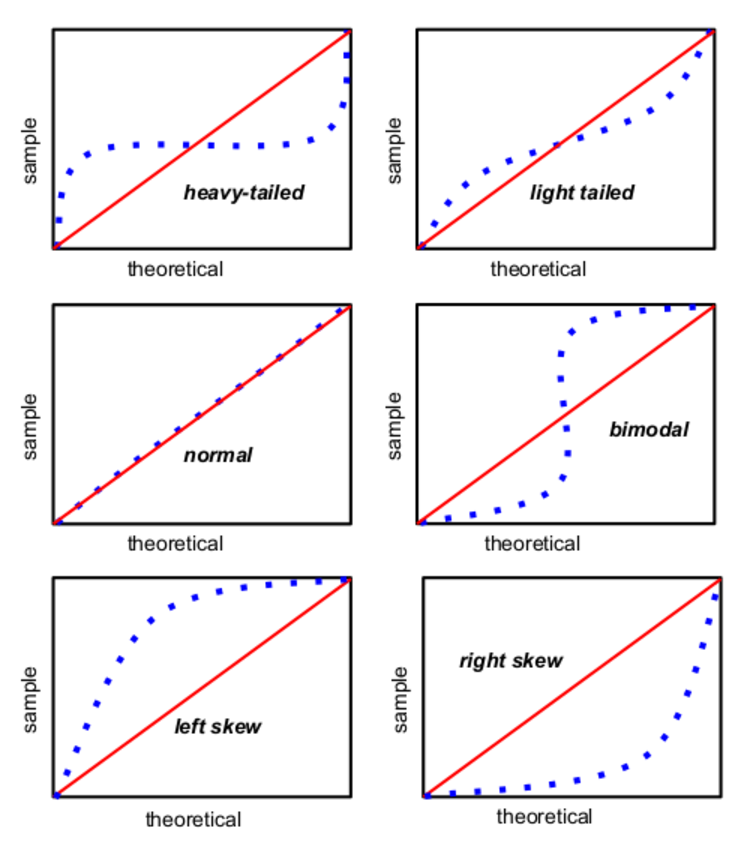
\includegraphics[width=0.6\textwidth]{figures/ch2/qqplot-tutorial}
	\caption{ How information about may be extracted from QQplots.}
	\label{fig:qqplot-tutorial}
\end{figure*}


Another way to analyze scaling characteristics is through QQplots. \acrshort{QQplot} is a visual method to compare sample data with a specific stochastic distribution. It orders the sample data values from the smallest to largest, then plots these values against the expected value given by the probability distribution function. The data sample values appear along the y-axis and the expected values along the x-axis. The more linear, the more the data is likely to be expressed by this specific stochastic distribution. 

Depending on how the plot behaves, some features of the empirical dataset compared to the theoretical can be observed. Figure~\ref{fig:qqplot-tutorial} presents a summary.


%%%%%%%%%%%%%%%%%%%%%%%%%%%%%%%%%%%%%%%%%%%%%%%%%%%%%%%%%%%%%%%%%%%%%%%%%%%%%%%%
\subsection{QoS/QoE Related Metrics}


For the point of view of traffic generation, QoS and QoE metrics should present similar values to the ones found in real scenarios. As stated by Magyesi and Szabó\cite{validate-trafficgen}, important QoS/QoE metrics on validation of workload tools are Round trip Time values (\acrshort{RTT}), average queue waiting time and, queue size. Still, on queue size, self-similar traffic consumes router buffers faster than Poisson traffic\cite{multi-player-online-game-self-similarity}.

%%%%%%%%%%%%%%%%%%%%%%%%%%%%%%%%%%%%%%%%%%%%%%%%%%%%%%%%%%%%%%%%%%%%%%%%%%%%%%%%
\section{Conclusions}


In this chapter, we discussed some fundamental concepts of our research: network traffic generators, network traffic modeling, and network traffic generators validation. In section~\ref{sec:traffic-gen}, we surveyed types of traffic generators and a comparison between their considerable variability of features. It helped us to summarize and have an understanding of what is available nowadays for use, and define the gaps. Also, this chapter helped us to identify what tools and frameworks are available to use. Section~\ref{sec:modeling-traffic} showed a brief overview of efforts on network traffic modeling and realistic traffic generation. In the modeling issue, was presented a short historical summary of some critical points of network traffic modeling, and on practical traffic generation, discussing some reference tools.



%%%%%%%%%%%%%%%%%%%%%%%%%%%%%%%%%%%%%%%%%%%%%%%%%%%%%%%%%%%%%%%%%%%%%%%%%%%%%%%%
\chapter{Architecture and Methods}\label{ch:architecture}
%%%%%%%%%%%%%%%%%%%%%%%%%%%%%%%%%%%%%%%%%%%%%%%%%%%%%%%%%%%%%%%%%%%%%%%%%%%%%%%%

In this chapter, we will present our tool which aims to fill the gaps addressed in chapter~\ref{ch:introduction}. \textit{SIMITAR} is an acronym for \textbf{\textit{SnIffing, ModellIng, and TrAffic geneRation}}\footnote{A Scimitar or Scymitar is curved sword, originating in the Middle East\cite{scymitar-sword}.}. This acronym summarizes its operation.
SIMITAR is a traffic generator able to \textbf{\textit{learn}} features of real traffic automatically, and reproduce synthetic traffic similar to the original. It records a model for the traffic in an \acrshort{XML}\footnote{Extensible Markup Language (XML) is a markup language that defines rules for storing and processing hierarchical data\cite{web-xml}.} file we call the \textit{Compact Trace Descriptor}(CTD file) as input-data SIMITAR can use, \textit{pcap} files or real-time captures. 

\begin{figure*}[ht!]
    \centering
    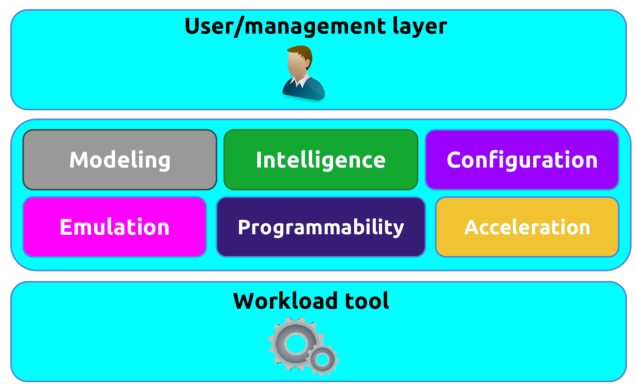
\includegraphics[height=2.4in]{figures/ch1/layer-diagram}
    \caption{ Architecture conceptual idea: a toll to automatize many tasks on traffic modelling and generation.}
    \label{fig:layer-diagram}
\end{figure*}

In figure~\ref{fig:layer-diagram} we abstract our stated concepts in a layer model diagram. Our tool works as an intermediate layer which offers traffic \textbf{\textit{modeling}}, \textbf{\textit{configuration}}, \textbf{\textit{emulation}}, and \textbf{\textit{programmability}}. In the figure, we also include packet acceleration\footnote{Packet acceleration is a concept introduced by DPDK\cite{web-dpdk}, which means kernel by-pass. Packet acceleration optimizes the packet processing, and therefore traffic generation, enabling higher throughput rates.}, which is not implemented yet but discussed as future work, in chapter~\ref{ch:conclusion}.  We are going to refer to the underlying workload tool as the packet generator engine and it is used via API by SIMITAR. 

We are also introducing the concept of \textit{programmability}. The user may create custom traffic, creating the \textit{Compact Trace Descriptor}, following its template. The idea is that he or she can create custom traffic in a platform agnostic way, without having to study any documentation, and implement any script or program.  Using a component methodology, we uncouple the packet generation, from the data collection and parameterization process. We developed it using the factory design pattern\footnote{Design patterns are abstractions that aim to help the implementation and systems structuring\cite{web-design-patterns}.} to make the extension easy for any packet generator engine. 

We abstract its whole operation cycle in figure~\ref{fig:cycle-of-operation}. Our tool collects packet data from live captures or pcap files. It then breaks down the traffic into flows and uses the data to generate parameters for our traffic model. Finally, SIMITAR provides these parameters to a packet generator engine and controls the packet injection.

% cycle of operation
\begin{figure*}[ht!]
        \centering
        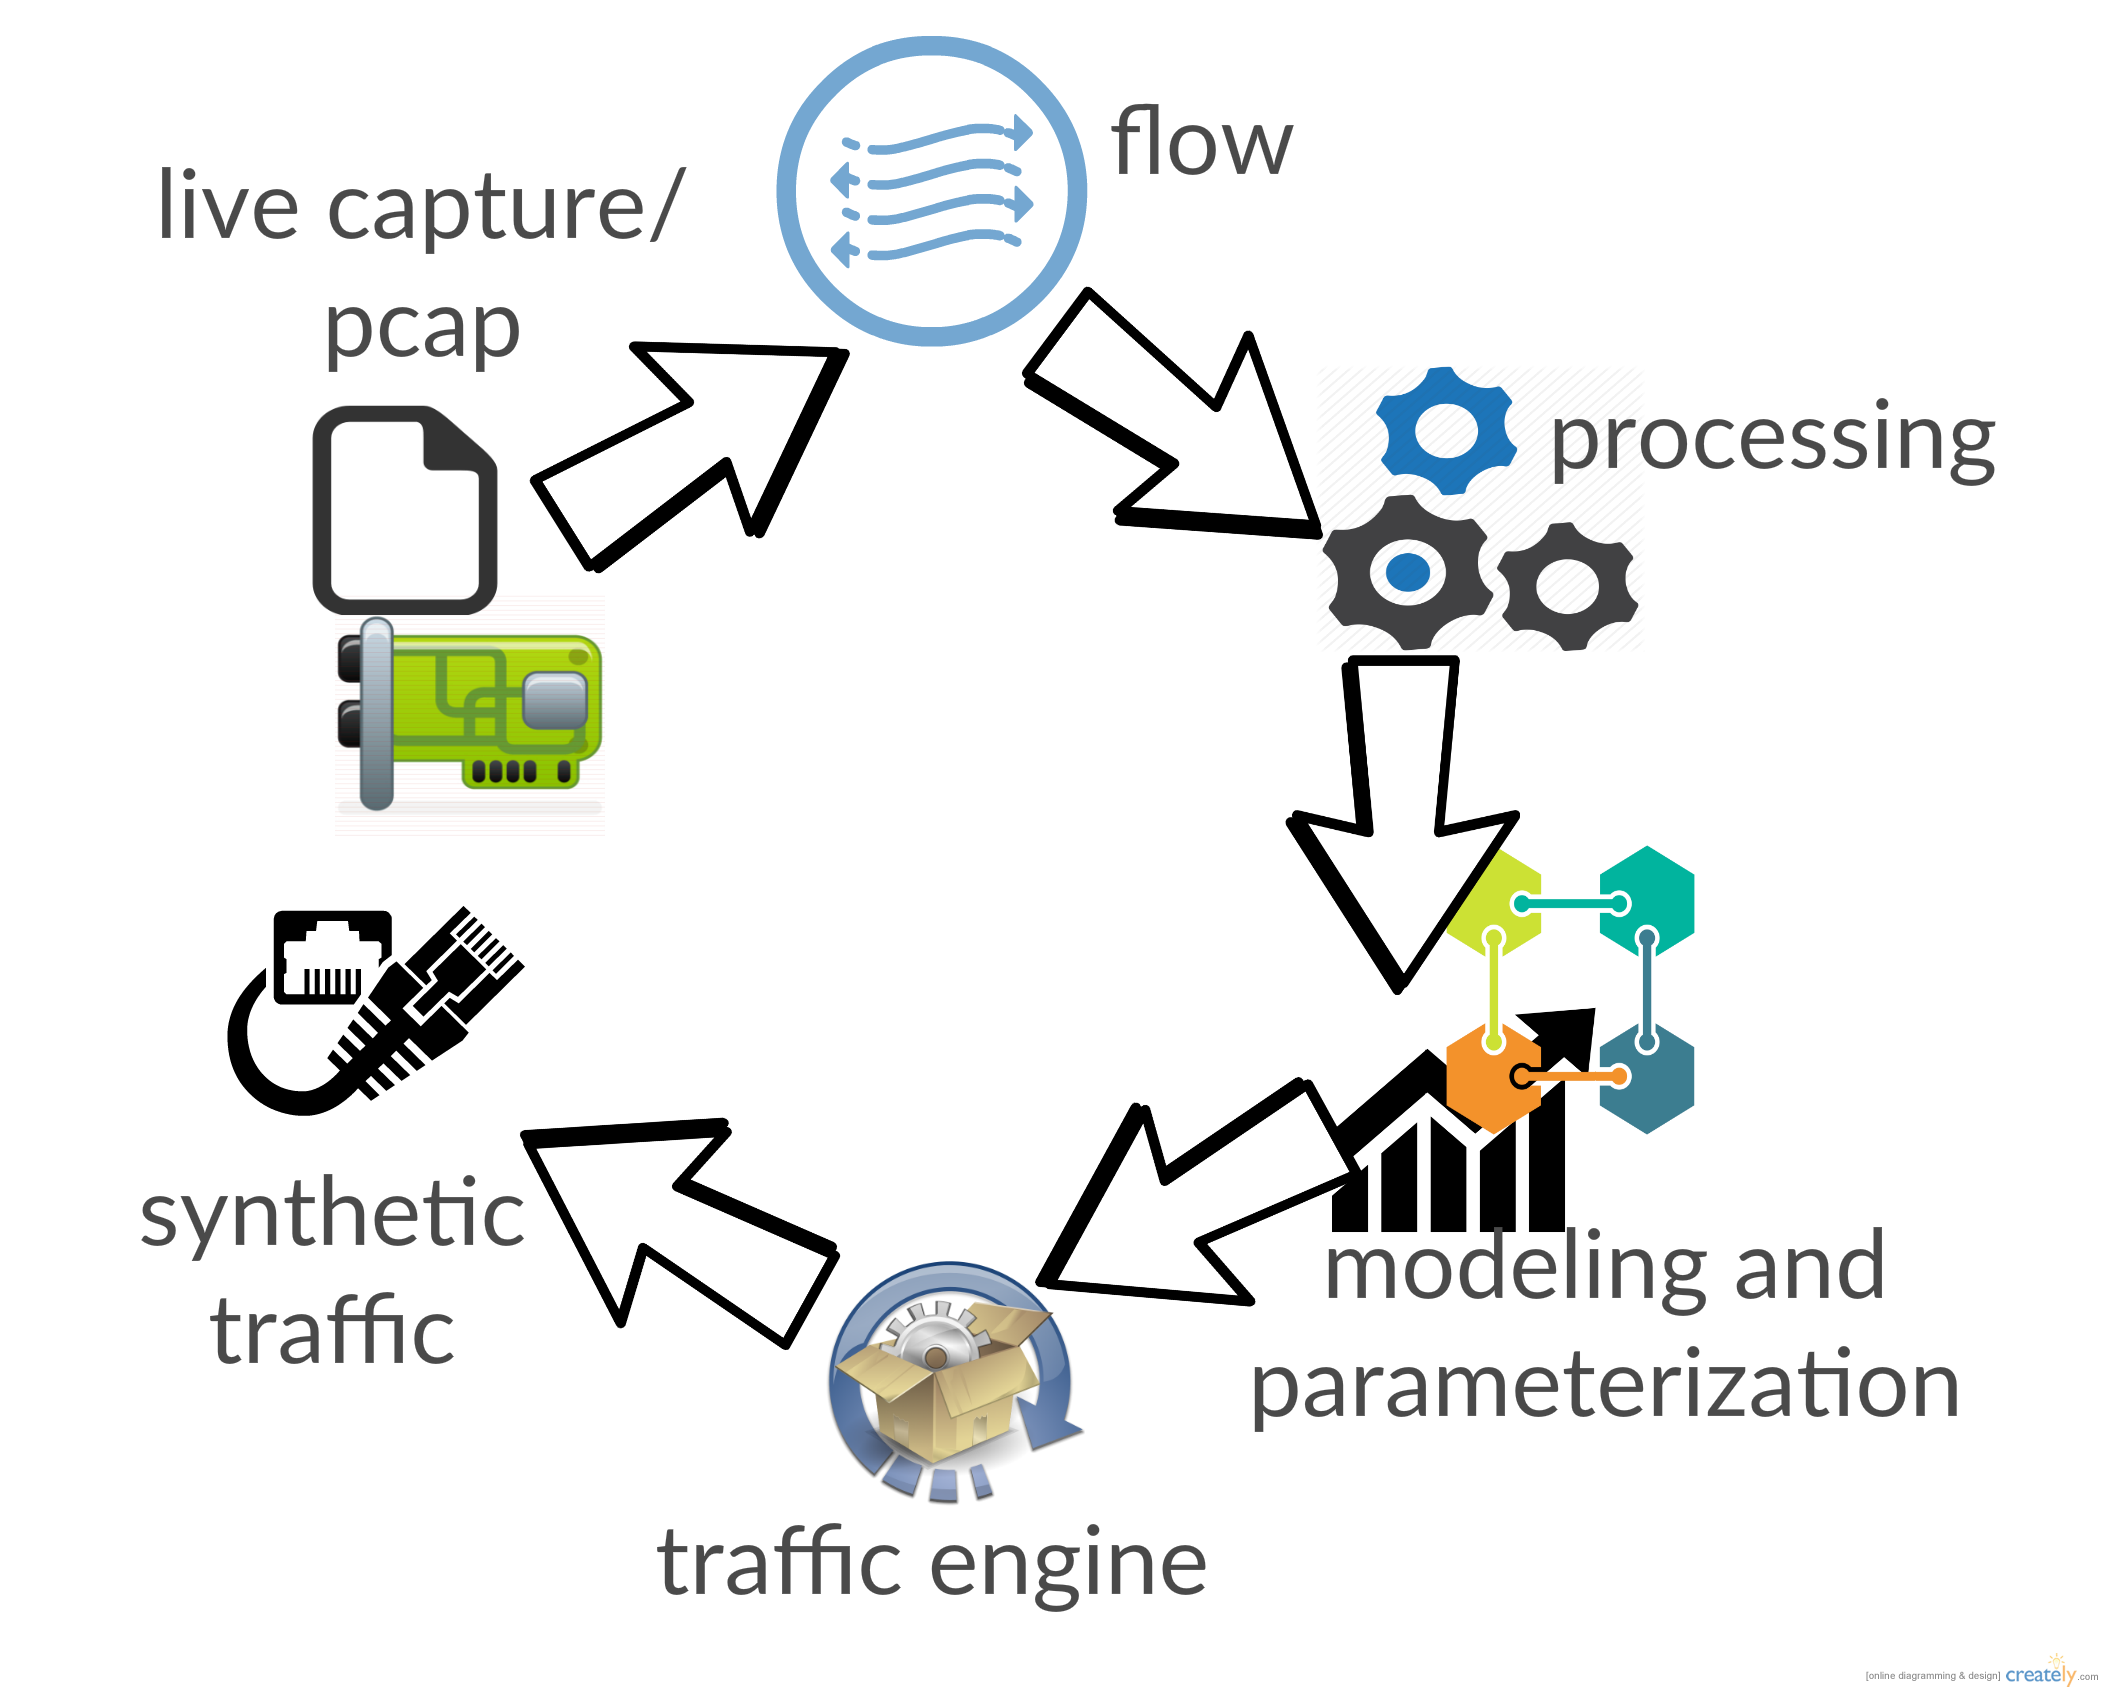
\includegraphics[height=3.0in]{figures/ch3/digram-project-cycle}
        \caption{This figure represents an operation cycle of SIMITAR, emphasizing each main step: sniffing, flow classification, data storing, data processing and fitting, model parameterization,  and synthetic traffic generation.}
    \label{fig:cycle-of-operation}
\end{figure*}

%%%%%%%%%%%%%%%%%%%%%%%%%%%%%%%%%%%%%%%%%%%%%%%%%%%%%%%%%%%%%%%%%%%%%%%%%%%%%%%%
\section{SIMITAR Architecture Overview}

The SIMITAR architecture is shown in figure~\ref{fig:architecture}. It is composed of four components: a \textbf{\textit{Sniffer}}, an \textbf{\textit{SQLite database}}, a \textbf{\textit{Trace Analyzer}}, a \textbf{\textit{Flow Generator}}. We describe each part below.

% component diagram and module design
\begin{figure*}[ht!]
        \centering
        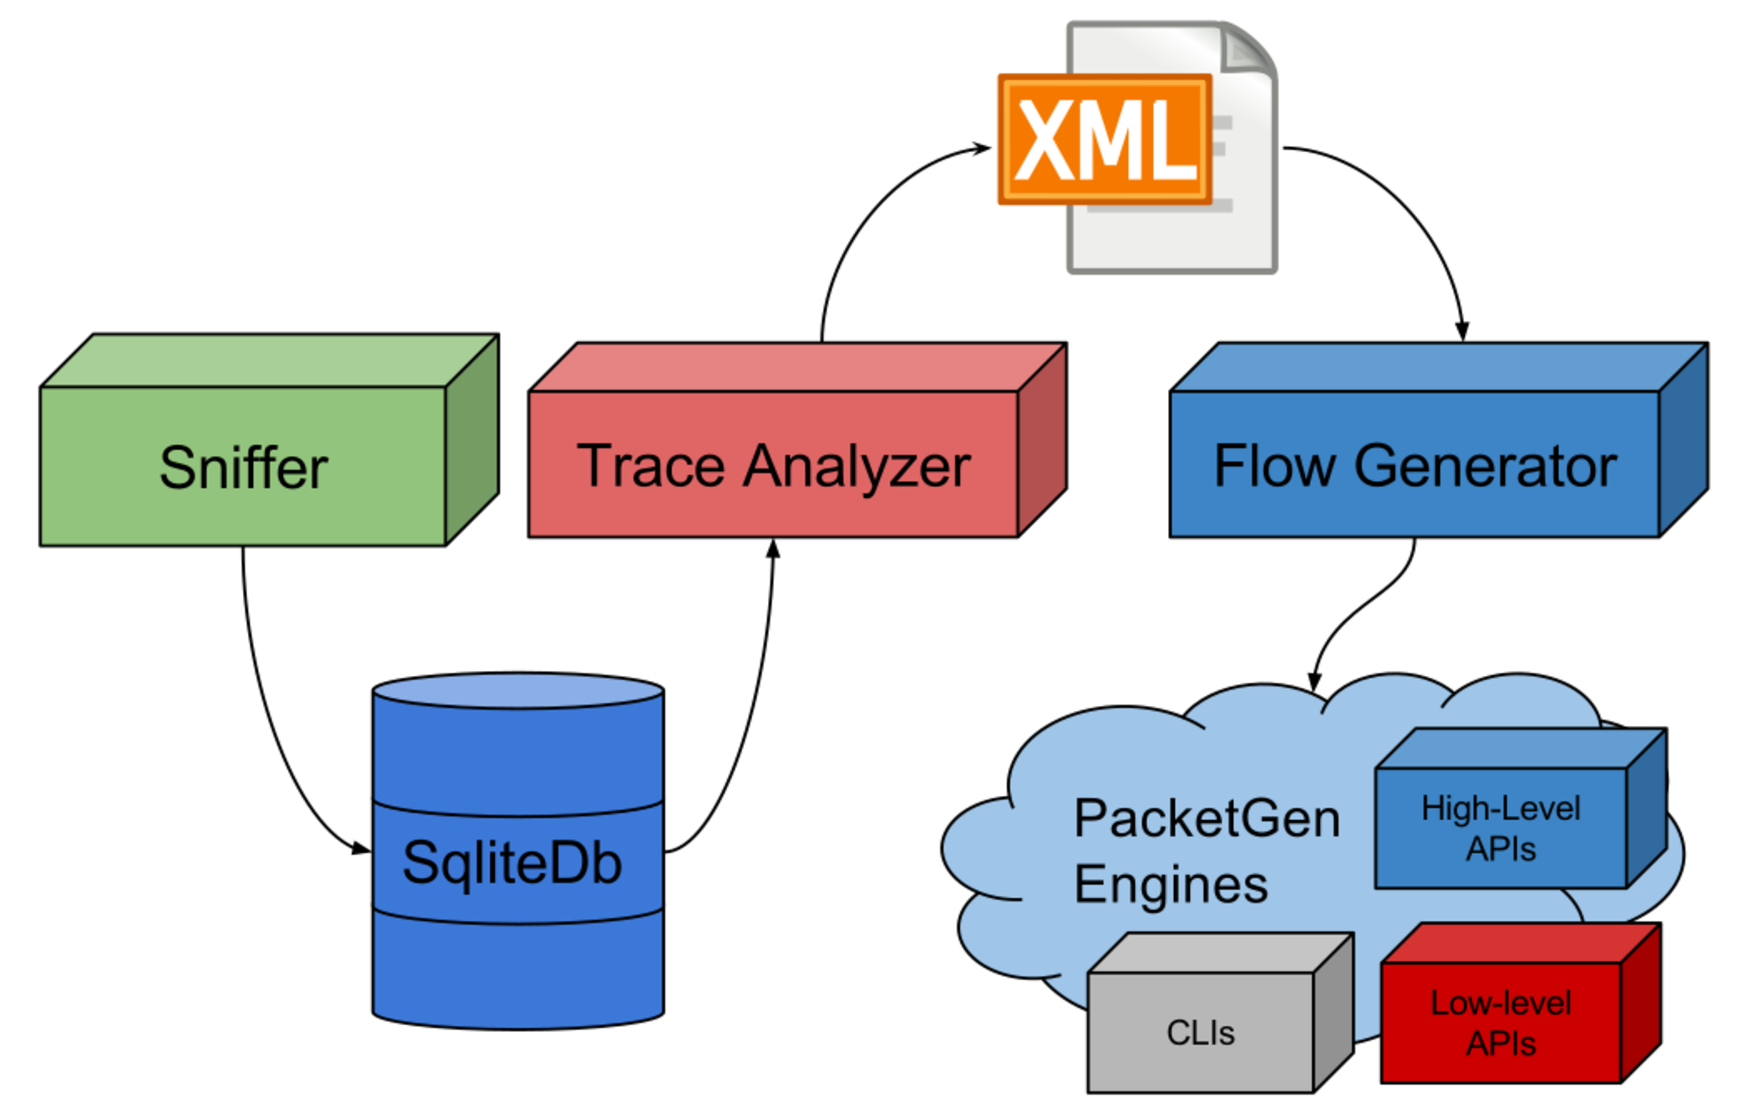
\includegraphics[height=2.7in]{figures/ch3/architecture-diagram}
        \caption{Architecture of SIMITAR}
    \label{fig:architecture}
\end{figure*}

%%%%%%%%%%%%%%%%%%%%%%%%%%%%%%%%%%%%%%%%%%%%%%%%%%%%%%%%%%%%%%%%%%%%%%%%%%%%%%%%
\section{ \textit{Sniffer} }


A sniffer is a tool that can intercept and analyze internet packets from a given network interface. Our \textit{Sniffer} component collects network traffic data and classifies it into flows, storing it on an SQLite database. It uses header field matches to classify the flows, such as in SDN switches\cite{sdn-survey}. The fields used  are:

\begin{itemize}
\item Link Protocol
\item Network Protocol
\item Network Source and Destination Address
\item Transport Protocol
\item Transport Source and Destination Port
\end{itemize}


\begin{figure*}[ht!]
        \centering
        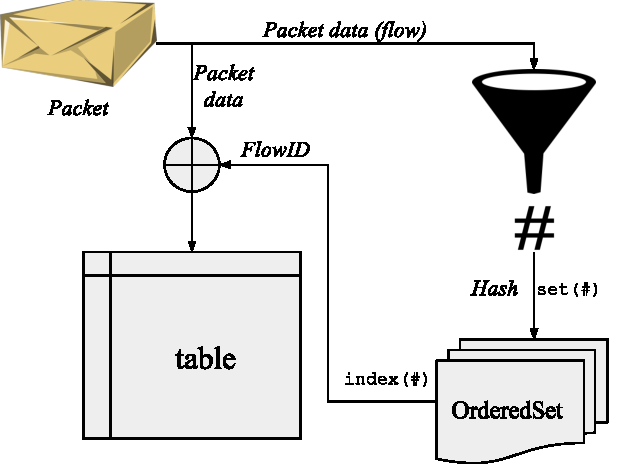
\includegraphics[height=2.5in]{figures/ch3/sniffer-classifier}
        \caption{SIMITAR's sniffer hash-based flow classification}
    \label{fig:sniffer}
\end{figure*}



We implemented the first version of this component in Shell Script (Bash). Tshark\cite{web-tshark} was used to extract header fields, and Awk to match the flows, and Sed/Awk to create the SQLite queries. This version was too slow to operate in real time on ethernet interfaces. On the other hand, this approach was fast to implement and enabled the implementation of the other components. The second and current version is in Python. This version used Pyshark\cite{web-pyshark} as a sniffer library.

The \textit{Sniffer} has a data structure we developed called \textit{OrderedSet}. A set is a list of elements with no repetition but does not keep track of the insertion order. Our \textit{OrderedSet} does. Also, it uses a 64 bit hash function from the \acrshort{FNV}\footnote{The collision probability of a good 64 bits hash function in a table with 10000 items is about of $2.71e-12$.} family. The listed header fields are inputs for a hash function. The hash value is added to the ordered set which returns its order (index on the \textit{OrderedSet}). We chose its value as packet \acrshort{flowID}.

%c++ http://ideone.com/F0V42m
As future improvements for this component, we propose a more efficient implementation in C++ and data visualization for the collected data. In this way, we can optimize packet processing. We discuss this in more depth in chapter~\ref{ch:conclusion}.

%%%%%%%%%%%%%%%%%%%%%%%%%%%%%%%%%%%%%%%%%%%%%%%%%%%%%%%%%%%%%%%%%%%%%%%%%%%%%%%%
\section{ \textit{SQLite database} }

\begin{figure*}[ht!]
        \centering
        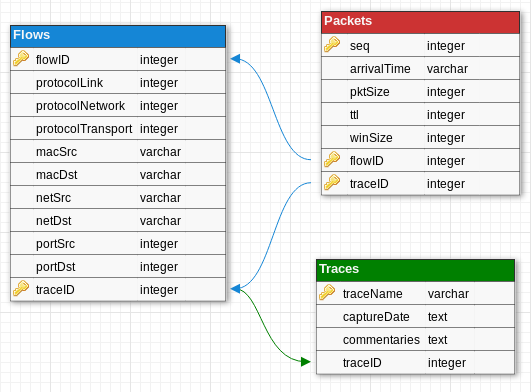
\includegraphics[height=3.0in]{figures/ch3/database-relational-model}
        \caption{SIMITAR's SQLite database relational model}
    \label{fig:simitar-database}
\end{figure*}




The database stores the collected raw data from the traces for further analysis. The \textit{Sniffer} records data on it and the  \textit{Trace Analyzer} reads. We choose an SQLite database because according to its specifications\cite{web-sqlite}, it fits our purposes well. It is simple and suitable for an amount of data smaller than terabytes. In figure~\ref{fig:simitar-database}, we present the relational model of our database, which stores a set of features extracted from packets, along with the flowID calculated by the \textit{Sniffer} component.


%%%%%%%%%%%%%%%%%%%%%%%%%%%%%%%%%%%%%%%%%%%%%%%%%%%%%%%%%%%%%%%%%%%%%%%%%%%%%%%%
\section{ \textit{Trace Analyzer} }


This module is the core of our project. It creates a trace model via the analysis of the collected data. The \textit{Trace Analyzer} has the task to learn these features from raw trace data (stored in the SQLite database) and generate an XML file to store a parameterized model. A \textit{Compact Trace Descriptor} (CTD) acts as a human and machine-readable file, which describes a traffic trace through a set of flows, each of them represented by a set of parameters, such as header information and analytical models. In figure~\ref{fig:CTD-diagram} we show a directory diagram of a CDT file. It has many flow fields, and each one contains each estimated parameter . We will now describe how we constructed it.


\begin{figure}
\centering
\subfloat[]{
  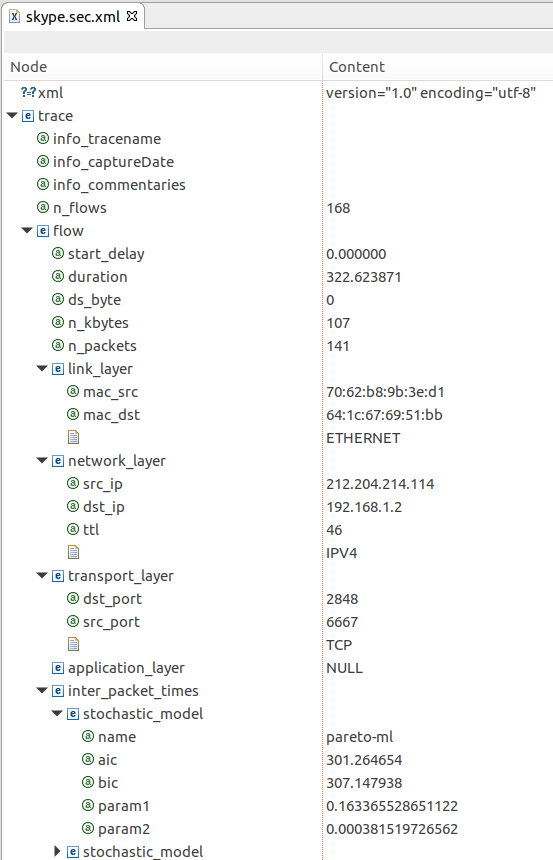
\includegraphics[height=4.in]{figures/ch3/cdt1}
}
\subfloat[]{
  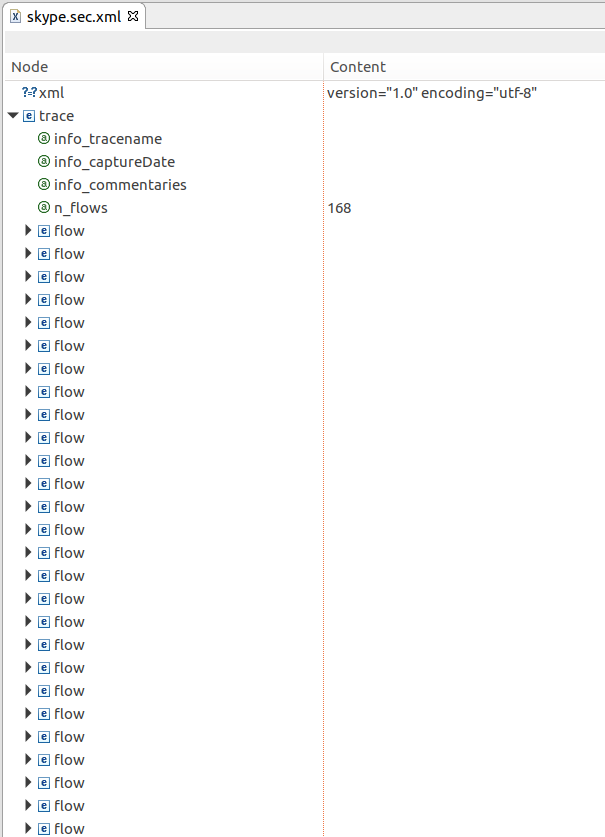
\includegraphics[height=4.in]{figures/ch3/cdt2}
}
\caption{Directory diagram of the schema of a Compact Trace Descriptor (CDT) file. On the left, we present a dissected flow, and on the right a set of flows.}
\label{fig:CTD-diagram}
\end{figure}


%%%%%%%%%%%%%%%%%%%%%%%%%%%%%%%%%%%%%%%%%%%%%%%%%%%%%%%%%%%%%%%%%%%%%%%%%%%%%%%%
\subsection{Flow features}

We measured some flow-features directly from data. They are:

\begin{itemize}
\item Flow-level properties like duration of flow, start delay, number of packets per flow, number of KBytes per flow;
\item Header fields, like protocols, QoS fields, ports, and addresses.
\end{itemize}

Each one of these parameters is unique to each flow. Other features like packet-size distribution and inter-packet times follow probability distributions. To represent these characteristics, we used sets of stochastic-based models.

%%%%%%%%%%%%%%%%%%%%%%%%%%%%%%%%%%%%%%%%%%%%%%%%%%%%%%%%%%%%%%%%%%%%%%%%%%%%%%%%
\subsection{Inter-Packet Times}


\begin{figure*}[ht!]
    \centering
    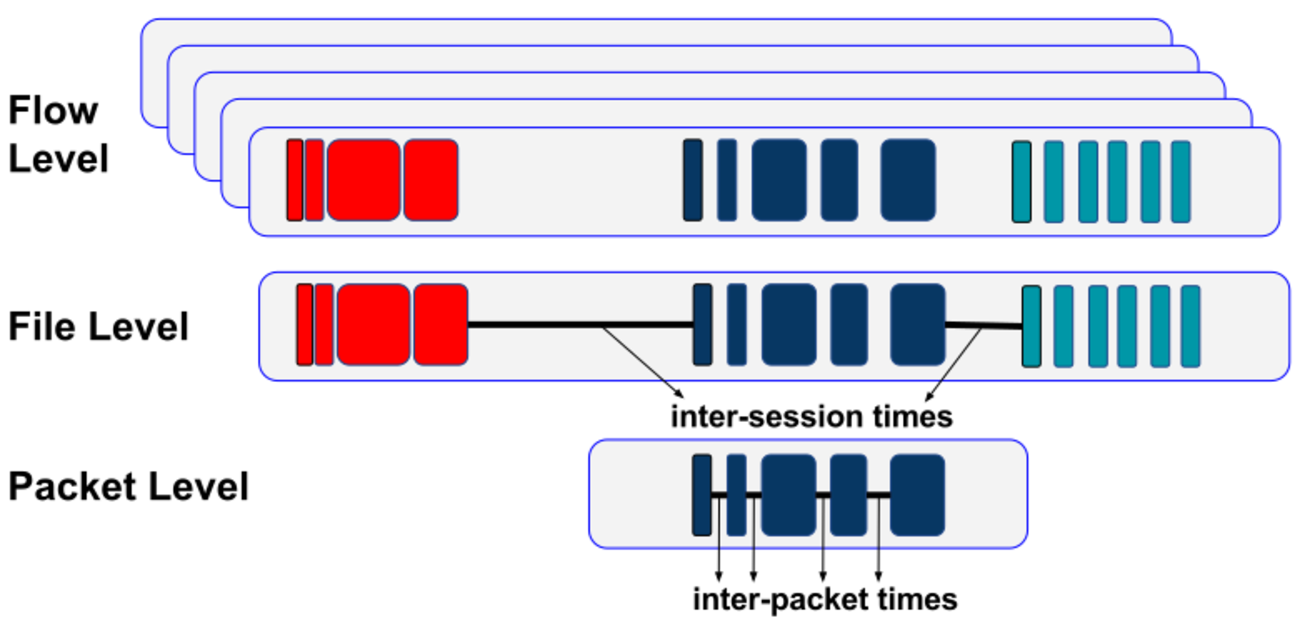
\includegraphics[height=2.0in]{figures/ch3/modified-harpoon-model}
    \caption{The schema of the modified version of the Harpoon algorithm we adopt on SIMITAR.}
    \label{fig:modified-harpoon-model}
\end{figure*}


To represent inter-packet times, we adopted a modified version of the Harpoon’s traffic model. An in-depth explanation of the original model can be found at  \cite{harpoon-paper} and \cite{harpoon-validation}. Harpoon uses a definition of each level, based on the measurement of \acrshort{SYN} and \acrshort{ACK} TCP flags. It uses TCP flags (SYN) to classify packets at different levels, naming their file, session, and user level. We chose to estimate these values, based on inter-packet times only. The distinction is made based on the time delay between packets. For our purposes, the advantage of our strategy is that the evaluation of the packet-train is not attached to a specific header field so that we can define packet trains for any flow. We illustrate this behavior in figure~\ref{fig:modified-harpoon-model}.

In our algorithm, we defined three different layers of data transference to model and control: \textit{file}, \textit{session}, and \textit{flow}. For SIMITAR, a file is a sequence of consecutive packets transmitted continuously, without a long interruption of traffic. A file can be, for example, packets from a download, a UDP connection or a single \acrshort{ICMP} echo packet. The session-layer refers to a sequence of multiple files transmitted between a source and a destination, belonging to the same flow. The flow level refers to the conjunction of flows, as classified by the \textit{Sniffer}. Now, we will explain SIMITAR operation for each layer.

In the \textbf{flow-layer}, the \textit{Trace Analyzer}  loads the flow arrival times from the database and calculates the inter-packet times within the flow context. At the session layer, we used a deterministic approach for evaluating file transference time and times between files: ON/OFF times sequence for packet trains. We chose a deterministic model because in this way we can express diurnal behavior. We developed an algorithm called \texttt{calcOnOff} that estimates these times. It also determines the number of packets and bytes transferred for each file. Since the ON times will serve as input for actual traffic generators, we defined a minimum acceptable time for on periods equal to 100 ms. ON times can be arbitrary and small, and they could be incompatible with acceptable ON periods for traffic generators. Also in the case of just one packet, the ON time would be zero. So  a minimum acceptable time was set to solve these issues. The OFF times, on the other hand, are defined by the constant \texttt{session\_cut\_time}\footnote{In the code it is called \texttt{DataProcessor::m\_session\_cut\_time} }. If the time between two packets of the same flow is greater than \texttt{session\_cut\_time}, we consider them belonging to a different file, so this time is a session OFF time. In this case, we use the same value of the constant \textit{Request and Response timeout} of Swing\cite{swing-paper} for the \texttt{session\_cut\_time}: 30 seconds. The control of ON/OFF periods in the traffic generation is made by the \textit{Flow Generator} component\footnote{This control is made by the class \texttt{NetworkFlow}}.

In the \textbf{file-layer}, we modeled the inter-packet times at the file level. We selected all times smaller than \texttt{session\_cut\_time} 9, and all files within the same flow were considered to follow the same model. We delegated the control of the inter-packet times to the underlying packet generator engine. We ordered them, from the best to the worst. Currently, we are using eight different stochastic functions parameterizations. We display each of them in table~\ref{tab:parameterizations-sumary} .

\begin{table}[ht!]
	\centering
	\caption{Functions and parameterizations used by SIMITAR}
		\begin{tabular}{c c c c}
			\toprule
			\textbf{Function} & Linear Regression & Maximum Likelihood & Empirical\footnotemark \\
			\midrule
			Weibull         & $\checkmark$    &                  &                  \\
			Normal             &                  &                  &  $\checkmark$    \\
			Exponential      & $\checkmark$    &                  &  $\checkmark$    \\
			Pareto          & $\checkmark$    & $\checkmark$    &                  \\
			Cauchy          & $\checkmark$    &                  &                  \\
			Constant          &                 &                  & $\checkmark$    \\
			\bottomrule
		\end{tabular}
		\label{tab:parameterizations-sumary}
\end{table}
\footnotetext{Empirical estimation, by calculation of the avarge, and standard deviation} 


From the functions presented in the first column in table~\ref{tab:parameterizations-sumary}, Weibull, Pareto, and Cauchy are heavy-tailed (and self-similar processes). However, if the flow has less than 30 packets, just the constant model is evaluated. It is because numerical methods gave poor results if the data sample is small. We sorted these models according to the Akaike Information Criterion (AIC) as default\cite{sourcesonoff-paper}\cite{bic-aic-comparision}. This methodology is explained in-depth in chapter~\ref{ch:modeling-evaluation} and illustrated in figure 10.  All these constants and modes of operation are modifiable via command-line options.

\begin{figure*}[ht!]
    \centering
    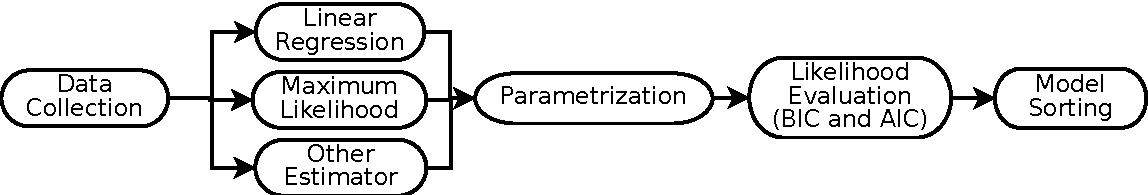
\includegraphics[height=0.9in]{figures/ch3/simitar-parametrization}
    \caption{Diagram of parameterization and model selection for inter-packet times and inter-file times.}
    \label{fig:model-parameterization}
\end{figure*}

%%%%%%%%%%%%%%%%%%%%%%%%%%%%%%%%%%%%%%%%%%%%%%%%%%%%%%%%%%%%%%%%%%%%%%%%%%%%%%%%
\subsection{Packet Sizes}


Our approach for the packet size was much simpler. Since the majority of packet size distributions found in real measurements are bi-modal\cite{packet-distribution-model}\cite{sourcesonoff-paper}\cite{udp-flows-model}, we first sorted all packet sizes of flow into two modes. We defined a packet-size cut value of 750 bytes, the same value adopted by\cite{udp-flows-model}.

We knew how many packets each mode has, and then we fitted a model to it. We use three stochastic models: constant, exponential and normal. Since self-similarity does not make sense for packet-sizes, we prefered to use just the simpler models. When there was no packet for a model, we set a flag \texttt{NO\_MODEL}, and when there was only a single packet, we used the constant model. Then we calculated the $BIC$ and $AIC$ for each, but we decided to set the constant model as the first.

As is possible to see in many works\cite{packet-distribution-model} \cite{udp-flows-model}, since the standard deviation of each mode tends to be small, constant fittings give good approximations. Also, it is computationally cheaper for the traffic generated than the other models, since no calculation is needed for each packet sent. Since both $AIC$ and $BIC$ criteria will always select the constant model as the worst, we decided to ignore this.

%%%%%%%%%%%%%%%%%%%%%%%%%%%%%%%%%%%%%%%%%%%%%%%%%%%%%%%%%%%%%%%%%%%%%%%%%%%%%%%%
\subsection{ \textit{Compact Trace Descriptor} }


An example of the final result of all the methods is presented in the XML code below. The code illustrates a single flow from a \textit{Compact Trace Descriptor}(CDT) file. The inter-packet times' models are on tags "\texttt{inter\_packet\_times}" and the packet trains models on tags "\texttt{session\_times}". All the times are in seconds, and "\texttt{inf}" represents infinity. The protocol of each layer is on the data field for each tag. 


\begin{minted}[frame=single,
               framesep=3mm,
               linenos=true,
               xleftmargin=21pt,
               tabsize=4,
               fontsize=\scriptsize, 
               breaklines=true]{xml}
    <flow start_delay="0.144400" duration="317.744333" ds_byte="0" n_kbytes="40" n_packets="344">
        <link_layer mac_src="64:1c:67:69:51:bb" mac_dst="70:62:b8:9b:3e:d1">ETHERNET</link_layer>
        <network_layer src_ip="192.168.1.1" dst_ip="192.168.1.2" ttl="64">IPV4</network_layer>
        <transport_layer dst_port="2128" src_port="53">UDP</transport_layer>
        <application_layer>DNS</application_layer>
        <inter_packet_times>
            <stochastic_model name="pareto-ml" aic="-1165.310696" bic="-1157.646931" param1="0.405085202535192" param2="0.002272655895996"/>
            <stochastic_model name="pareto-lr" aic="-454.049749" bic="-446.385984" param1="0.061065000000000" param2="0.002272655895996"/>
            <stochastic_model name="weibull" aic="-246.882037" bic="-239.218273" param1="0.120355000000000" param2="0.001629000000000"/>
            <stochastic_model name="exponential-me" aic="486.370061" bic="494.033826" param1="1.340057495455104" param2="0.000000000000000"/>
            <stochastic_model name="normal" aic="1629.370900" bic="1637.034665" param1="0.746236637899171" param2="2.626808289821357"/>
            <stochastic_model name="exponential-lr" aic="3166.816047" bic="3174.479812" param1="0.009752000000000" param2="0.000000000000000"/>
            <stochastic_model name="cauchy" aic="31737.418442" bic="31745.082207" param1="0.000000000000194" param2="-3152.827055696396656"/>
            <stochastic_model name="constant" aic="inf" bic="inf" param1="0.746236637899171" param2="0.000000000000000"/>
        </inter_packet_times>
        <session_times on_times="29.22199798,73.40390396,151.84077454" off_times="30.85738373,32.42027283" n_packets="19,103,222" n_bytes="2272,12399,26689"/>
        <packet_sizes n_packets="344" n_kbytes="40">
            <ps_mode1 n_packets="344" n_kbytes="40">
                <stochastic_model name="constant" aic="inf" bic="inf" param1="120.232558" param2="0.000000"/>
                <stochastic_model name="normal" aic="2926.106952" bic="2933.788235" param1="120.232558" param2="16.941453"/>
                <stochastic_model name="exponential-me" aic="3987.126362" bic="3994.807645" param1="0.008317" param2="0.000000"/>
            </ps_mode1>
            <ps_mode2 n_packets="0" n_kbytes="0">
                <stochastic_model name="no-model-selected" aic="inf" bic="inf" param1="0.000000" param2="0.000000"/>
            </ps_mode2>
        </packet_sizes>
    </flow>
\end{minted}


%%%%%%%%%%%%%%%%%%%%%%%%%%%%%%%%%%%%%%%%%%%%%%%%%%%%%%%%%%%%%%%%%%%%%%%%%%%%%%%%
\section{ \textit{Flow Generator} }

\begin{figure*}[pht!]
    \centering
    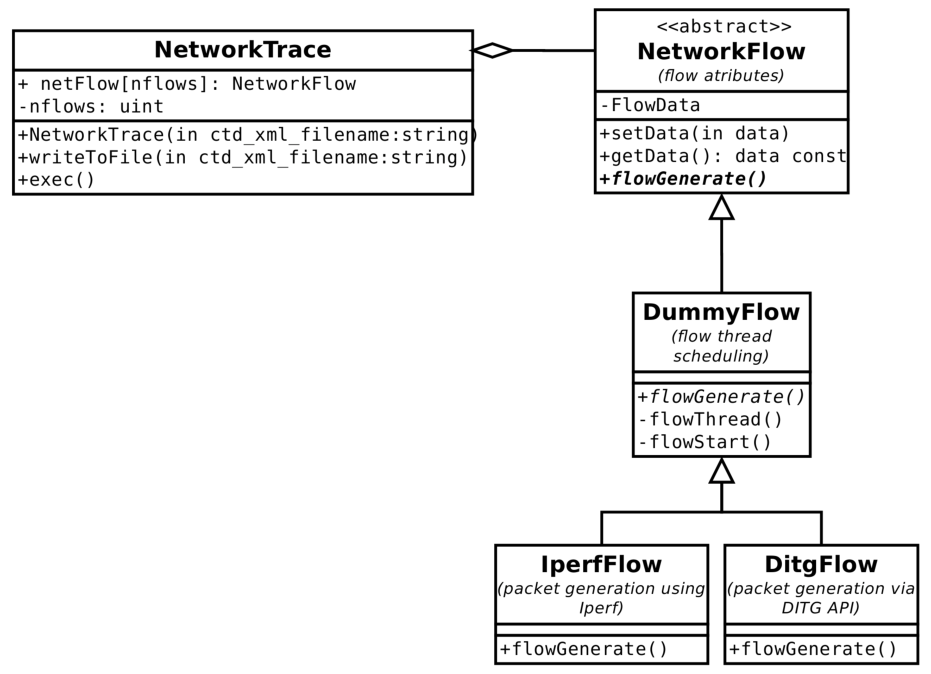
\includegraphics[height=3.0in]{figures/ch3/trace-flow}
    \caption{Class hierarchy of NetworkTrace and NetworkFlow, which enables the abstraction of the traffic generation model of the packet generation engine.}
    \label{fig:network-trace-flow-class-diagram}
\end{figure*}

\begin{figure*}[pht!]
    \centering
    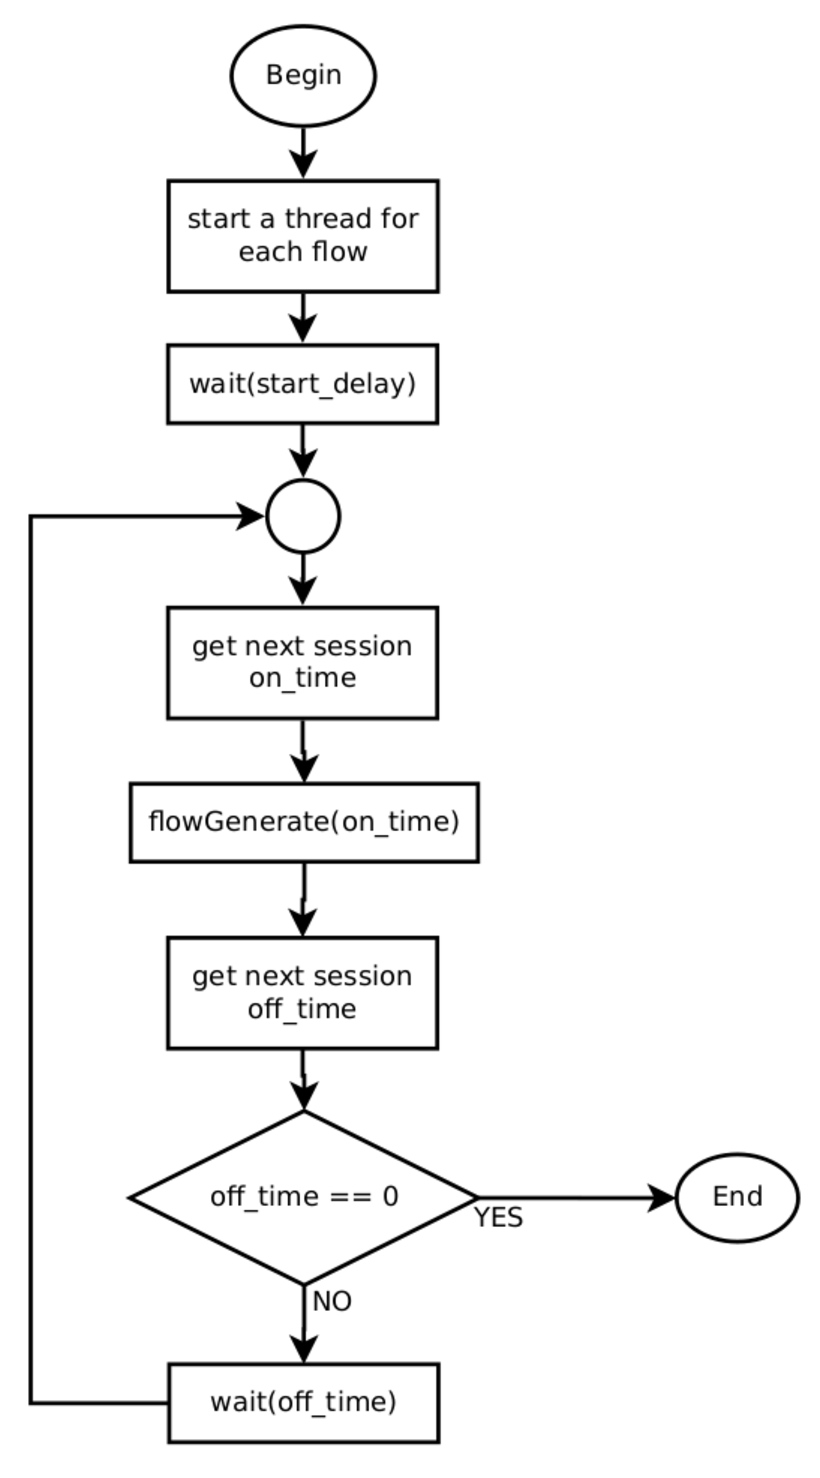
\includegraphics[height=4.5in]{figures/ch3/alg-simplified-harpoon}
    \caption{Simplified-harpoon emission algorithm}
    \label{fig:alg-simplified-harpoon}
\end{figure*}


\begin{figure*}[pht!]
    \centering
    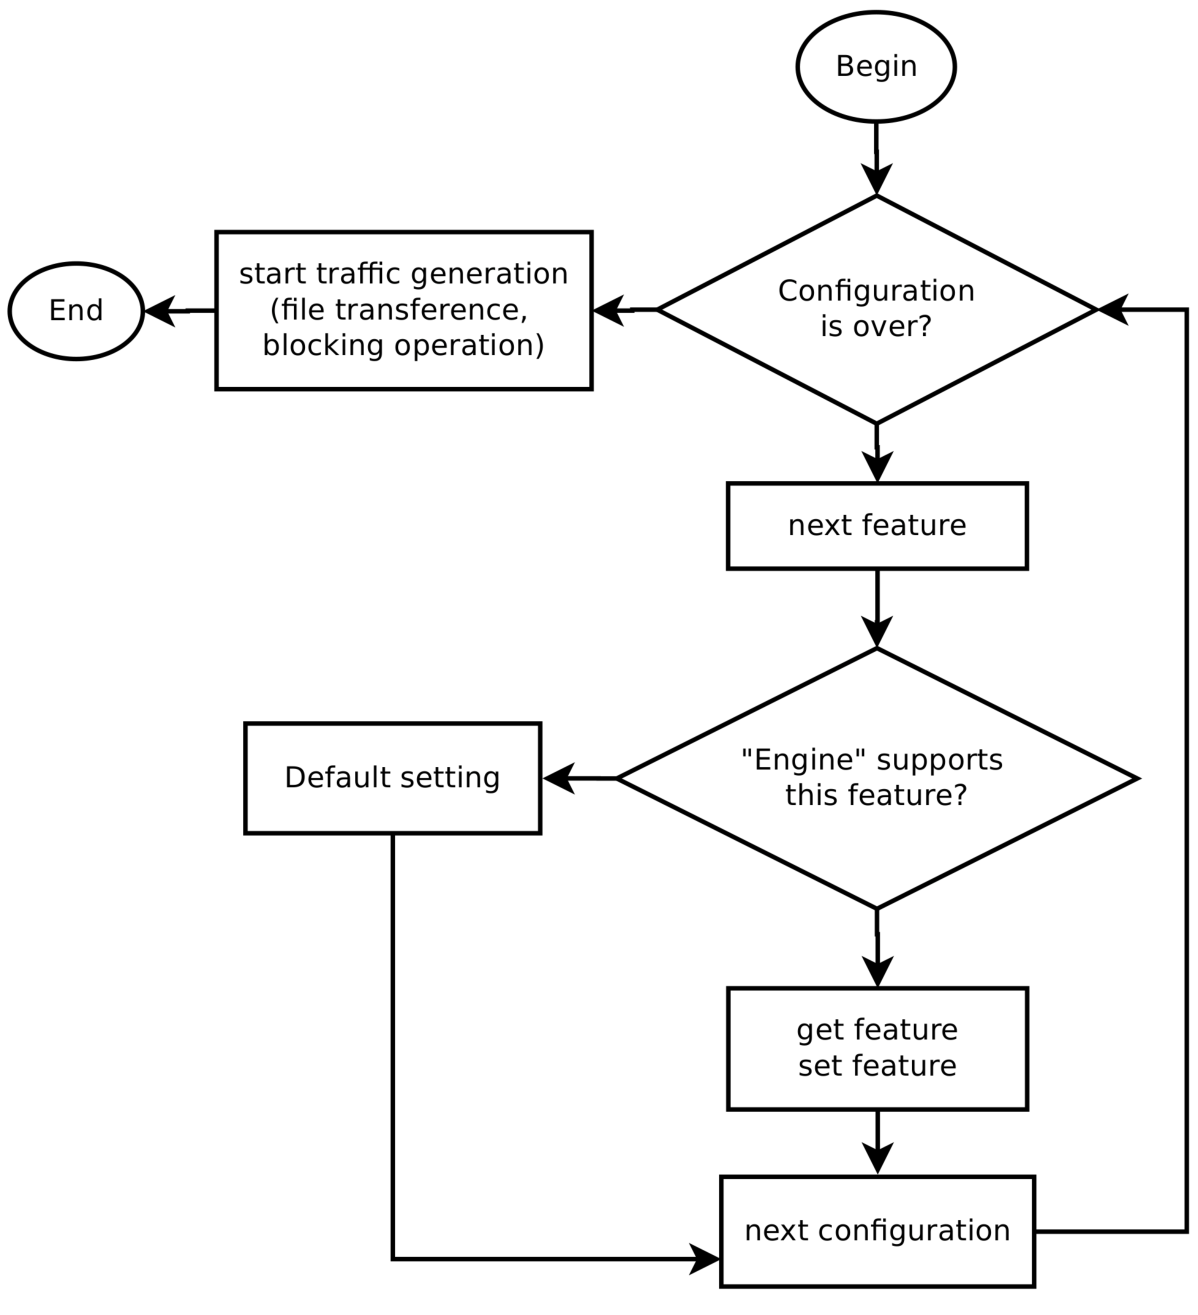
\includegraphics[height=4.0in]{figures/ch3/alg-traffic-engine-config}
    \caption{Packet engine configuration method}
    \label{fig:alg-traffic-engine-config}
\end{figure*}



The \textit{Flow Generator} handles the data on the \textit{Compact Trace Descriptor} file, and is used to retrieve parameters for traffic generation. It crafts and controls each flow in a separate thread. We have already implemented this component using Iperf and Libtins(C++ API)\cite{web-libtins} as packet generators. It must follow the class hierarchy as presented in figure~\ref{fig:network-trace-flow-class-diagram}. This component was designed using the factory design pattern, to simplify its expansion and support\footnote{
If the user wants to introduce support for a new packet generator engine, he has to implement a derived class of \texttt{DummyFlow}, such as in figure~\ref{fig:network-trace-flow-class-diagram}. In the current release of SIMITAR, we already have \texttt{IperfFlow} and \texttt{TinsFlow}, and \texttt{DitgFlow}. This new class needs to be static, and the support must be implemented on the factory \texttt{NetworkFlowFactory}.
For closed loop packet-crafters (the ones that need to establish a connection to generate traffic), two methods must be implemented: \texttt{flowGenerate()} and \texttt{server()}. \texttt{flowGenerate()} is responsible for sending a single file, as defined on de figure~\ref{fig:modified-harpoon-model}. The \texttt{server()} methods must implement the reception of $n$ files. For open-loop packet crafters (the ones whose just inject packets but do not establishes a connection), such as the one we implemented using Libtins, does not need the server-side implemented. }


This component itself is a multi-layer workload generator according to the typing introduced in chapter~\ref{ch:literature-review}\footnote{Since it works both at packet and flow level, but does not work at application level yet.}. At the flow-level, SIMITAR controls each flow using the algorithm in figure~\ref{fig:alg-simplified-harpoon}. This algorithm handles our model as defined in figure~\ref{fig:modified-harpoon-model}. This procedure is independent of the underlying packet crafting tool used. It starts a \textit{thread} for each flow in the \textit{Compact Trace Descriptor}, and then the thread sleeps for \texttt{start\_delay} seconds. The \texttt{start\_delay} is the arrival time of the first flow packet. Passed this time, it then calls the underlying packet generator tool (defined as command line argument), and passes to it the flowID, file ON time, number of packets and number of bytes to be sent (file size), and network interface. Then it sleeps until the next session OFF time. When the list of ON/OFF times from the flow is over, the thread ends.


At the packet level, SIMITAR configures the packet-generator tool to send a \textit{file}, as defined in figure~\ref{fig:modified-harpoon-model}. This method must use the available parameters, attributes and \textit{getters} to configure and generate thread-safe traffic using the method \texttt{flowGenerate()}. The \textit{file} configuration must follow figure~\ref{fig:alg-traffic-engine-config}. Down below we present a simple code of how the D-ITG API can be used to generate packet-level traffic. A more complex configuration is possible, but it serves to illustrate the procedure. We call this concept \textit{Flow Generation Programming}. Its API documentation is available at the D-ITG website\footnote{\href{http://www.grid.unina.it/software/ITG/manual/index.html\#SECTION00047000000000000000}{http://www.grid.unina.it/software/ITG/manual/index.html\#SECTION00047000000000000000}}.

\begin{minted}[frame=single,
               framesep=3mm,
               linenos=true,
               xleftmargin=21pt,
               tabsize=4,
               fontsize=\scriptsize, 
               breaklines=true]{c++}


// This implementation is just a simplified version to illustrate the procedure.
void DitgFlow::flowGenerate(const counter& flowId, const time_sec& onTime, const uint& npackets, const uint& nbytes,  const string& netInterface)
{
    // create command to generate the traffic
    std::string strCommand;
    std::string localhost = getNetworkSrcAddr(); 
    strCommand += " -t " + std::to_string(onTime); 
    strCommand += " -k " + std::to_string(nbytes / 1024);
    strCommand += " -a " + getNetworkDstAddr();
    
    // configure protocol
    if (this->getTransportProtocol() == PROTOCOL__TCP)
        strCommand += " -T TCP -D ";
    else if (this->getTransportProtocol() == PROTOCOL__UDP)
        strCommand += " -T UDP ";
    else if (this->getTransportProtocol() == PROTOCOL__ICMP)
        strCommand += " -T ICMP ";
        
    //configure inter-packet time model, just Weibull or Constant
    StochasticModelFit idtModel;
    for(uint i = 0;;i++)
    {    
        idtModel = this->getInterDepertureTimeModel(i);
        if(idtModel.modelName() == WEIBULL)
        {
            strCommand += " -W " + std::to_string(idtModel.param1()) + " " + std::to_string(idtModel.param2());
            break;
        }
        else if ( idtModel.modelName() == CONSTANT)
        {
            strCommand += " -C " + std::to_string(nbytes/(1024*onTime));
            break;
        }
    }
    
    // it uses C strings as arguments
    // it is not blocking, so it must block until finishes
    int rc = DITGsend(localhost.c_str(), command.c_str()); // D-ITG API
    usleep(onTime*10e6); // D-ITG uses miliseconds as time unity
    if (rc != 0)
    {
        PLOG_ERROR << "DITGsend() return value was" << rc ; // our log macro for erros
        exit(EXIT_FAILURE);
    }
}
\end{minted}


%%%%%%%%%%%%%%%%%%%%%%%%%%%%%%%%%%%%%%%%%%%%%%%%%%%%%%%%%%%%%%%%%%%%%%%%%%%%%%%%
\section{Network Packet Generator}


A network packet generator is a tool or library that should provide its API or script interface for the \textit{Flow Generator} component. With this engine, the user must be able to send packets and control attributes such as sending time, bandwidth, number of packets, protocols, and so on. This means, any available parameter form the \textit{Compact Trace Descriptor}.


%%%%%%%%%%%%%%%%%%%%%%%%%%%%%%%%%%%%%%%%%%%%%%%%%%%%%%%%%%%%%%%%%%%%%%%%%%%%%%%%
\section{Usage and Use Cases}


SIMITAR is composed of three main command-line applications, whose give command line access to the \textit{Sniffer}, \textit{Trace Analyzer} and \textit{Flow Generator}, respectively:
\begin{itemize}
\item \texttt{sniffer-cli.py};
\item \texttt{trace-analyzer};
\item \texttt{simitar-gen} (the actual traffic generator). 
\end{itemize}

Below we show some usage commands of SIMITAR’s components. The \texttt{sniffer-cli.py} application creates a new trace entry on the database using the command option new. Then the \textit{Trace Analyzer} can create a \textit{Compact Trace Descriptor} using the same trace entry. We can change the constants used by the \textit{Trace Analyzer} by the command line option. As a traffic generator (\texttt{simitar-gen}), SIMITAR may work as a client or a server. Working as a server is necessary for closed-loop packet-generator engines; tools that require establishing a connection before generating the traffic, such as Iperf and D-ITG. It will just work passively. Working as a client it is acting as a traffic emitter. Open loop packet-crafter tools such as Libtins do not require server operation to send the traffic. In the case of closed-loop tools, the destination IP addresses must be explicitly given in the command line by the options \texttt{--dst-list-ip} or \texttt{--dst-ip}.


\begin{minted}[frame=single,
               framesep=3mm,
               linenos=true,
               xleftmargin=21pt,
               tabsize=4,
               fontsize=\scriptsize, 
               breaklines=true]{bash}

# @ SIMITAR/, load enviroment variables
source data/config/simitar-workspace-config.sh

# @ SIMITAR/sniffer/, execute to sniff the eth0 interface, and create a trace entry called "intrig" in the database
./sniffer-cli.py new intrig live eth0

# @ SIMITAR/sniffer/, execute this command to list all traces recorded in the database
./sniffer-cli.py list

# @ SIMITAR/trace-analyzer/, execute this command to create two Compact Trace Descriptors, called intrig.ms.xml and intrig.sec.xml. The first is parameterized using milliseconds, and de second uses seconds as time unity.
./trace-analyzer --trace intrig

# @ SIMITAR/simitar-gen/, execute these commands to generate traffic using the intrig.sec.xml compact trace descriptor. It is stored at the directory "../data/xml/". 
# Libtins
./simitar-gen --tool tins --mode client --ether eth0 --xml ../data/xml/intrig.sec.xml 
# Iperf
./simitar-gen --tool iperf --mode client --ether eth0 --xml ../data/xml/intrig.sec.xml --dst-ip 10.0.0.2
./simitar-gen --tool iperf --mode server --ether eth0 --xml ../data/xml/intrig.sec.xml

\end{minted}


\begin{figure*}[ht!]
    \centering
    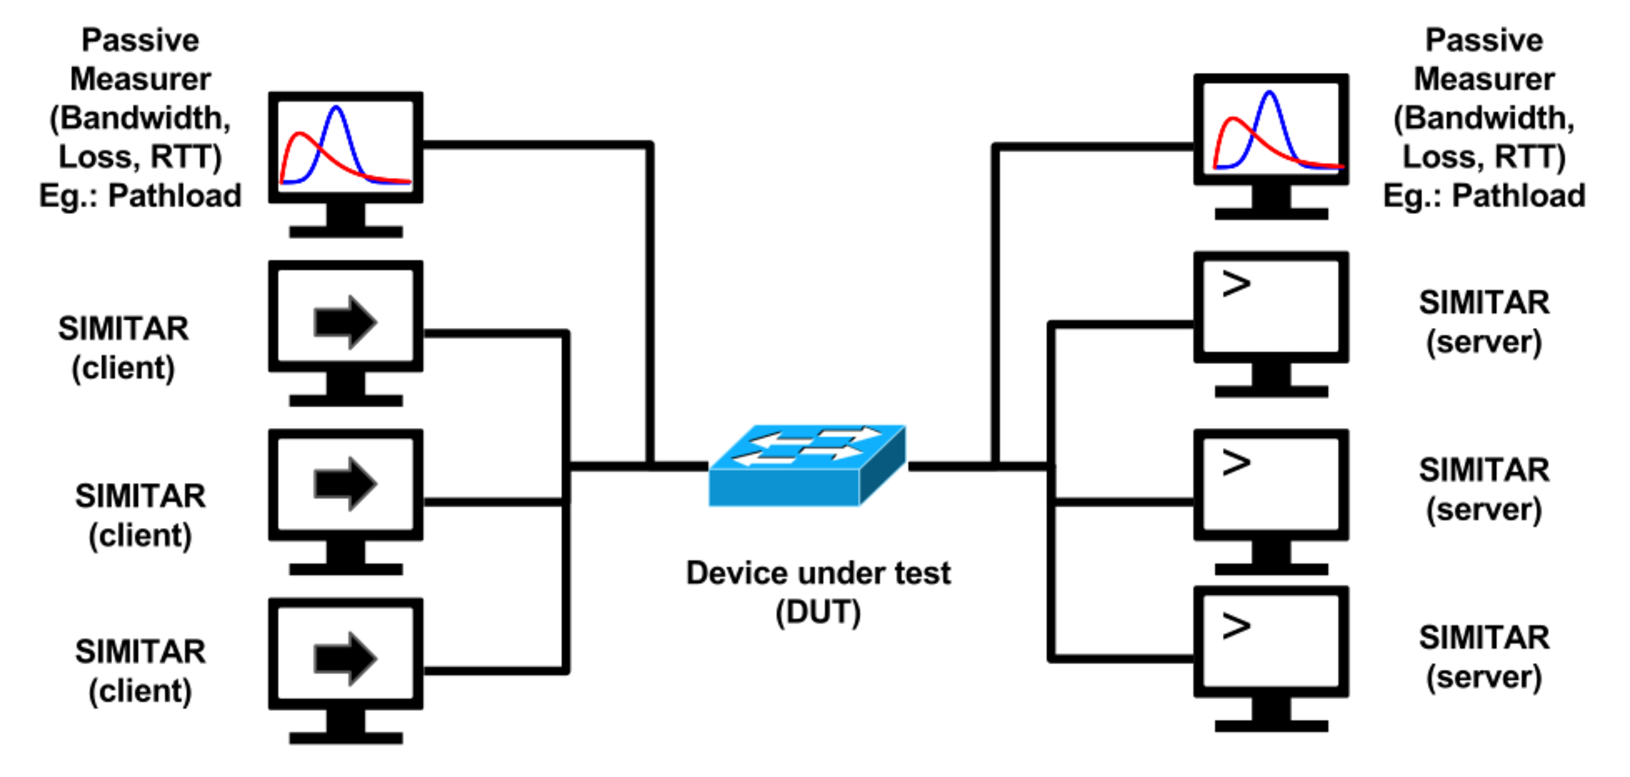
\includegraphics[height=2.4in]{figures/ch3/use-case}
    \caption{Use case example of SIMITAR}
    \label{fig:use-case}
\end{figure*}



Figure~\ref{fig:use-case} shows an example of a use case. A device under test can be stressed using a combination of traffic generated by many clients and server pairs. In the case of an open-loop packet generator tool (such as in the Libtins implementation), the servers and clients pairs are not necessary. Using passive network measures, such as Pathload\cite{web-pathload} and pathChirp\cite{swing-paper}\cite{web-pathchirp}, it is possible to measure statistics from the device under tests.

%%%%%%%%%%%%%%%%%%%%%%%%%%%%%%%%%%%%%%%%%%%%%%%%%%%%%%%%%%%%%%%%%%%%%%%%%%%%%%%%
\chapter{Modeling and Algorithms}\label{ch:modeling-evaluation}
%%%%%%%%%%%%%%%%%%%%%%%%%%%%%%%%%%%%%%%%%%%%%%%%%%%%%%%%%%%%%%%%%%%%%%%%%%%%%%%%


%%%%%%%%%%%%%%%%%%%%%%%%%%%%%%%%%%%%%%%%%%%%%%%%%%%%%%%%%%%%%%%%%%%%%%%%%%%%%%%%
\section{Introduction}


This chapter describes in-depth the implementation of the traffic modeling algorithms mentioned in Chapter 3. The first section gives a brief survey of other works that presented methodologies for a parameterizing stochastic process to describe internet traffic (inter-packet times and packet-trains). This introduction shows a scenario where there is no "one-fits-all" model. The best model always depends on the type of traffic. 

Many consolidate works investigate the nature of internet traffic, and many others on the modeling of stochastic functions for specific scenarios. However, there are not as many on model choice automation. In the second section, we discuss and cross-validate our methodology for automating the choice of inter-packet times processes. We select inter-packet times models using information criteria ($AIC$ and $BIC$) to rank the models from the best to the worst.  Since, to the best of our knowledge, there was no previous validation of the effectiveness of $AIC$ and BIC for ranking information criteria, we developed our cross-validation methodology to test their effectiveness.  

In the third section, we present our algorithm called "\texttt{calcOnOff}", a method to estimate packet trains periods (ON and OFF times) of an arbitrary flow, which do not rely on header fields, but just times between packets. Finally, the fourth section shows our strategy for guessing application protocols from flows, protocols using common transport header fields.


We use refer to two different cost functions on this chapter. The first is the Gadient Descendent Cost function, we refer as $J_\nabla$, since nabla ($\nabla$) is the notation used to represent gradients. The second is our cross-validation cost function, we refer as $J_M$, since it is used to rank stochastic models ($M$).


%%%%%%%%%%%%%%%%%%%%%%%%%%%%%%%%%%%%%%%%%%%%%%%%%%%%%%%%%%%%%%%%%%%%%%%%%%%%%%%%
\section{Literature Review on internet traffic modeling}


There are many works devoted to studying the nature of the Ethernet traffic\cite{selfsimilar-ethernet}. Classic Ethernet models used Poisson related processes to model traffic\footnote{In our study case we used two Poisson related processes, both using exponential distributions: Exponential(Me) and Exponential(LR). Exponential distributions are considered continuous versions of the Poisson process.  Since we are using time as a real number, we preferred to use just exponential distributions, for simplicity.}. A Poisson process represents the probability of events occur with a known average rate, and independently of the last occurrence\cite{book-poisson}. 

However, studies made by Leland et al.  showed that the Ethernet traffic has a self-similar and fractal nature. Even if they can represent the randomness of   Ethernet traffic, simple Poisson processes cannot express traffic "burstiness" on a long-term timescale, such as traffic "spikes" on long-range "ripples". These characteristics are an indication of the fractal and self-similar nature of the traffic, that usually we express by distributions with infinite variance, called heavy-tailed. Heavy-tail means that a stochastic distribution is not exponentially bounded\cite{sourcesonoff-paper}, and can guarantee self-similarity via Joseph and Noah effects\cite{selfsimilar-highvariability}. Examples of heavy-tailed functions are Weibull, Pareto, Cauchy. However, these distributions may guarantee self-similarity, but not necessarily they will ensure other features like good correlation and same average packet rate\cite{validate-trafficgen}. 

There are plenty of works in the literature which proposes processes and methodologies for modeling times between packets and packet trains\cite{selfsimilar-ethernet}\cite{analysis-self-similar}\cite{stochastic-selfsimilar}\cite{selfsimilar-highvariability}\cite{multi-player-online-game-self-similarity}\cite{estimation-renewal-function-ethernet-traffic}\cite{modelling-of-self-similar}\cite{empirical-interarrival-study}\cite{modeling-concurrent-heavy-tailed}\cite{optimal-scheduling-of-heavy-tailed-traffic}\cite{modelling-of-self-similar}. Fiorini\cite{modeling-concurrent-heavy-tailed}  presented a heavy-tailed ON/OFF model, which represented the traffic generated by many sources. The model emulated a multiple source power-tail Markov-Modulated (\acrshort{PT-MMPP}) ON/OFF process, where the ON times have been power-tail distributed. They achieve analytical performance measurements using Linear Algebra Queueing Theory. 

Kreban and Clearwater\cite{hierarchical-dynamics-interarrival-times}  presented a model for times between job submissions from multiple users over a supercomputer. They have shown that the Weibull probability functions can express well small and high values of inter-job submission times. They also have tested exponential, lognormal and Pareto distributions. The Exponential distribution has not represented well long-range values because of it had felt-off too fast. On the other hand, the Pareto problem was that it had felt too slow. Lognormal have fitted well small values, but its performance had been weak on larger ones. Kronewitter\cite{optimal-scheduling-of-heavy-tailed-traffic} has presented a model of scheduling traffic of many heavy-tail sources. On his work, he had used many Pareto sources to represent the traffic. To estimate Pareto shape (parameter $\alpha$) he had used linear regression.


%%%%%%%%%%%%%%%%%%%%%%%%%%%%%%%%%%%%%%%%%%%%%%%%%%%%%%%%%%%%%%%%%%%%%%%%%%%%%%%%
\section{Automatized selection of inter-packet times models using \textit{AIC} and \textit{BIC}}

\subsection{Cross-validation Methodology}

There many consolidate works which have investigated the nature of internet traffic, and many others that had proposed processes to describe network traffic on specific scenarios. But not as many on model choice automation.  We propose and evaluate the use of the information criteria $BIC$ (Bayesian Information Criterion) and $AIC$ (Akaike Information Criterion) as suitable methods for automated model selection for inter-packet times.  

We then define our cross-validation method based on a cost function $J_M$,  which is an aggregator of traditional and critical metrics used on validation of stochastic models and traffic generators: Correlation(quality of the model), Average inter packet-time (related with the traffic Throughput), and Hurst Exponent (traffic fractal level).  $J_M$ assign weights from the best to the worst representation for each property of each trace model by using randomly generated data with our stochastic fittings. Through this process, we choose the best-fitted traffic model under evaluation. Afterward, we compare the results achieved by $AIC$/$BIC$ and our cost function. Given the approach mentioned above, we show that $AIC$/$BIC$ methods provide an intelligent stochastic process selection strategy for inter-packet times models.
We summarize the validation process in the steps below:
\begin{enumerate}
\item We have selected many \textit{pcap} files, representing different types of network scenarios. We extracted from these files the list of inter-packet times.
\item Using a set of stochastic functions, and parameterization methods, we defined a list of candidate stochastic processes to represent the inter-packet time's distribution for each dataset.
\item For each dataset, $AIC$ and $BIC$  were used to rank the processes, from the best to the worst, for each dataset.
\item Using each process from step four,  we generated random data and estimated the cost function $J$. We have repeated the random data generation  30 times, and the parameters used on the cost function had ion had a confidence interval of 95\%. Finally, we have ranked the processes from the best to the worst for each dataset.
\item Finally, we had two independent rankings, the one we wanted to validate, and others based on the literature. We compared the results.
\end{enumerate}
  
We also present some \textit{QQplots}, to visually compare the random-generated data and the original data-set. 


\subsection{Datasets}


We will use four \textit{pcap} files, where three are publicly available, to enable the reproduction of the simulations described in this chapter. The first is a lightweight Skype capture, found in Wireshark wiki 2, located at https://wiki.wireshark.org/Samp\footnote{https://wiki.wireshark.org/}, located  at \href{https://wiki.wireshark.org/SampleCaptures}{https://wiki.wireshark.org/SampleCaptures}. The file name is \texttt{SkypeIRC.cap}. We will call this trace \textit{skype-pcap}. The second is a CAIDA\footnote{http://www.caida.org/home/}{http://www.caida.org/home/} capture, and we can found it at \href{https://data.caida.org/datasets/passive-2016/equinix-chicago/20160121-130000.UTC}{https://data.caida.org/datasets/passive-2016/equinix-chicago/20160121-130000.UTC}. Access to this file requires a login, so is required the creation and approval of a new account.  The pcap's file name is \texttt{equinix-chicago.dirB.20160121-135641.UTC.anon.pcap.gz}. We call it \textit{wan-pcap}\footnote{\acrshort{WAN} stands for Wide Area Network}.

The third we capture in our laboratory \acrshort{LAN}, through a period of 1 hour in a firewall gateway between our local and external network. We call it \textit{lan-firewall-pcap}. The fourth is a capture of a busy private network access point to the Internet, available online on TCPreplay website\footnote{ \href{http://tcpreplay.appneta.com/wiki/captures.html}{http://tcpreplay.appneta.com/wiki/captures.html}}, called \texttt{bigFlows.pcap}. We will refer to it \textit{lan-gateway-pcap}.

We retrieved inter-packet times from the traffic traces and divided them into two equally sized datasets. We split the data based on the index of the array we use to store. Odd-indexed elements have been used as a training dataset, and even-indexed for cross-validation; to avoid data over-fitting.


\subsection{Stochastic Processes Modeling and Selection}


\subsubsection{Stochastic Processes}

We have adopted five stochastic functions (\textbf{Weibull}, \textbf{Normal}, \textbf{Exponential}, \textbf{Pareto} and \textbf{Cauchy}), and three methods for parameters estimation: \textbf{Linear Regression}, \textbf{Direct estimation}, and \textbf{Maximum Likelihood}, totaling seven stochastic processes : 
\begin{enumerate}
\item \textbf{Weibull} via Linear Regression;
\item \textbf{Normal} via Direct Estimation;
\item Exponential via Direct Estimation, we refer as \textbf{Exponential(LR)};
\item Exponential via Linear Regression, we refer as \textbf{Exponential(MLH)};
\item Pareto via Linear Regression, we refer as \textbf{Pareto(LR)};
\item Pareto via Maximum Likelihood, we refer as \textbf{Pareto(MLH)};
\item \textbf{Cauchy} via Linear Regression.
\end{enumerate}



The data that have been used for modeling was the training dataset. $AIC$, $BIC$ and the cost function have used the cross-validation dataset. Since the time samples resolution used were of $10^{-6}$s, all values equal to zero had been set to $5\cdot10^{-8}$s, to avoid division by zero. To avoid divergence in tangent operation used  Cauchy linearization process, we have floor-limited and upper-limited the inter-packet CDF values by  $10^{-6}$ and $0.999999$, respectively. We implemented this prototype using Octave and Python. We upload all the code and data from these experiments on Github\cite{aic-bic-repo}. 


\subsubsection{Linear regression (Gradient descendant)}


Linear regression is a method for estimating the best linear curve in the format:

\begin{equation}
y = ax + b
\end{equation}

to fit a given data set. We can use linear regression to estimate parameters of a non-linear curve expressing it on a linear format. For example, the Weibull CDF for $t > 0$ is:

\begin{equation}
F(t|\alpha, \beta) = F(t) = 1 - e^{-(t/\beta)^{\alpha}}
\end{equation}

Manipulating the equation:

\begin{equation}
\alpha\ln{(t)} - \alpha\ln{(\beta)} = \ln{(-\ln{(1 - F(t))})}
\end{equation}

If we call $x = \ln{(t)}$ and $y = \ln{(-\ln{(1 - F(t))})}$, we found a linear equation, where  $a = \alpha$ and $b = -\alpha\ln{(\beta)}$. Having in hands an estimation of the empirical CDF of our data samples, we apply the $x$ and $y$ definitions to linearize the data.

Using the gradient descendant, we find an estimation of the linear coefficients: $\hat{a}$ and  $\hat{b}$.  Using the inverse function of linear factors, we see the Weibull estimated parameters  $\hat{\alpha}$ and $\hat{\beta}$.

\begin{equation}
\alpha = a
\end{equation}

\begin{equation}
\beta = e^{-(b/a)}
\end{equation}


The gradient descendent consists of minimizing a cost function $J_\nabla(\theta)$, whose value decrease if the approximation becomes better. We explain this procedure in the appendix ~\ref{ap:revision-probability}. In the figure~\ref{fig:linearization} we present as examples, the linearized data for the inter arrivals from the \textit{skype-pcap}, and in the figure~\ref{fig:cost} the cost convergence. Appendix ~\ref{ap:aditional-plots} presents a complete set of figures.

Applying the inverse equations of the linear coefficients ($\hat{\alpha} = \hat{a}$ and $\hat{\beta} = e^{-(\hat{b}/\hat{a})}$  \footnote{We use the hat symbol ( $ \widehat{} $ ) for estimated parameters}, we can estimate the Weibull distribution parameters. We can summarize this procedure, in these steps:

\begin{enumerate}
\item Linearize the stochastic CDF function $F(t)$.
\item Apply the linearized  $y = y(F(t))$ and $x = x(t)$ on the empirical CDF and times datasets, respectively.
\item Use Gradient Descendant algorithm to find linear coefficients a and b.
\item Apply the inverse equation of the linear coefficients, to determine the stochastic function parameters.
\end{enumerate}



In the parameters estimation (step 4), there is an exception, since the Pareto scale ($x_{m}$) is defined by the smaller time allowed. In table~\ref{tab:linearization-sumary} we present a summary of the used equations in the procedure. In this notation, the subscript $i$ means that it is applied to every value measured empirically.


\begin{table}[h!]
    \centering
    \caption{Linearized functions, and parameters estimators, used by the linear regression}
    \label{tab:linearization-sumary}
    \begin{tabular}{llllll}
        \hline
        Function    & Linearized $x$     & Linearized $y$                    & \multicolumn{2}{l}{Parameters Estimator}                               &  \\
        \hline
        Cauchy      & $x_i = t_i$        & $y_i = \tan{(\pi(F(t_i) - 1/2))}$ & $\hat{\gamma} = \frac{1}{\hat{a}}$ & $\hat{t_0} = - \frac{\hat{b}}{\hat{a}}$                      &  \\
        Exponential & $x_i = t_i$        & $y_i = \ln{(1 - F(t_i))})$        & \multicolumn{2}{l}{$\hat{\lambda} = -\hat{a}$}                                              &  \\
        Pareto      & $x_i = \ln{(t_i)}$ & $y_i = \ln{(1 - F(t_i))}$         & $\hat{\alpha} = -\hat{a} $         & $\hat{x_{m}} = \min_{i = 0, ..., m}\{x_{i}\}$ &  \\
        Weibull     & $x = \ln{(t)}$     & $y = \ln{(-\ln{(1 - F(t))})}$     & $\hat{\alpha} = \hat{a}$                 & $\hat{\beta} = e^{-(\hat{b}/\hat{a})}$                                   & \\
        \hline
    \end{tabular}
\end{table}


\begin{figure}[ht!]
\centering
\subfloat[Linearized interarrival data]{
  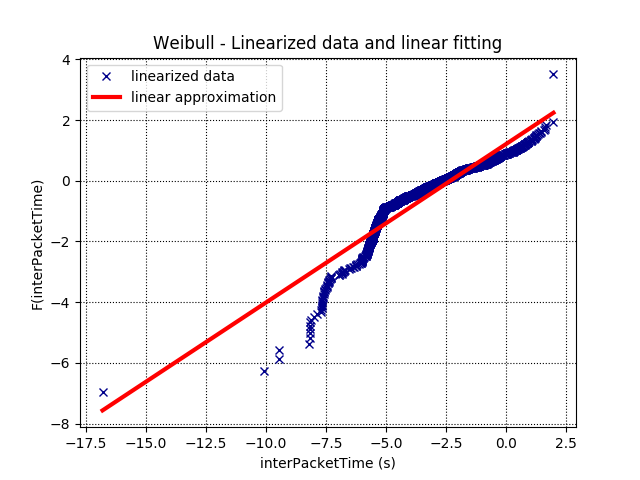
\includegraphics[height=50mm]{figures/apC/lr/Skype_Weibull_-_Linearized_data_and_linear_fitting}
  \label{fig:linearization}
}
%\hspace{0mm}
\subfloat[Cost function $J_\nabla$ of the linear regression]{
  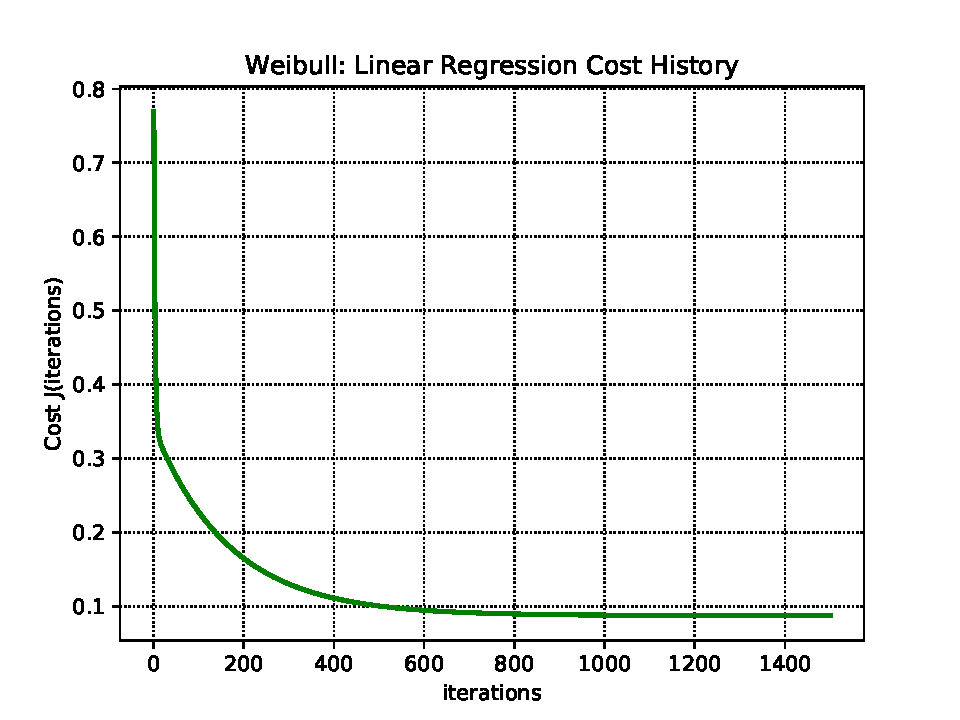
\includegraphics[height=50mm]{figures/apC/lr/Skype_Weibull_-_Cost_J(iterations)_convergence}
  \label{fig:cost}
}
\label{fig:linearization-cost}
\caption{Linearized data and cost function $J_\nabla$ of weibull linear regression}
\end{figure}


\subsubsection{Direct Estimation}

The expected value  $E(X)$ and variance $Var(X)$ of a random variable $X$ of some distributions are closely related to its parameters. Since the average $\bar{\mu}$ and its standard deviation$\bar{\sigma}$ are in general good approximations for the expected value and variance, we use them to estimate parameters.

Following the notation presented at table~\ref{tab:distributions-equations}, we have for the normal distribution the following ordered pair of parameters:

\begin{equation}
(\hat{\mu}, \hat{\sigma}) = (\bar{\mu}, \bar{\sigma})
\end{equation}

For the exponential distribution $E(X) = \frac{1}{\lambda}$. Therefore:

\begin{equation}
\hat{\lambda} = \frac{1}{\hat{\mu}}
\end{equation} 

\subsubsection{Maximum Likelihood}

The maximum likelihood estimation, is a method for estimation of The maximum likelihood estimation, is a method for estimation of The maximum likelihood estimation, is a method for estimation of parameters, winch maximizes the likelihood function. We explain in details this subject in Appendix~\ref{ap:revision-probability}. Using this method for the Pareto distribution;  it is possible to derive the following equations for its parameters: 


\begin{equation}
\hat{x_{m}} = \min_{i = 0, ..., m}\{x_{i}\}
\end{equation} 

\begin{equation}
\hat{\alpha} = \frac{n}{ \sum_{i = 0}^{m}(\ln{(x_{i}) - \ln(\hat{x_{m}})})  }
\end{equation} 

where $m$ is the sample(dataset) size.

\subsubsection{\textit{AIC} and \textit{BIC}}


Suppose that we have an statistical model $M$ of some dataset ${\boldsymbol{x} = \{x_1, ..., x_n}\}$, with $n$ independent and identically distributed observations of a random variable $X$. This model can be expressed by a PDF $f(x| \boldsymbol{\theta})$, where $\boldsymbol{\theta}$ a vector of parameter of the PDF, $\boldsymbol{\theta} \in \mathbb{R}^{k}$ ($k$ is the number of parameters). The  likelihood function  of this model $M$ is given by:

\begin{equation}
L(\boldsymbol{\theta}|\boldsymbol{x} ) =  f(x_1|\boldsymbol{\theta})\cdot...\cdot f(x_n|\boldsymbol{\theta}) = \prod_{i = 1}^{n}f(x_i|\boldsymbol{\theta})
\end{equation}

Now, suppose we are trying to estimate the best statistical model, from a set ${M_1, ..., M_n}$, each one whit an estimated vector of parameters  ${\boldsymbol{\hat{\theta_1}}}, ..., {\boldsymbol{\hat{\theta_n}}}$. $AIC$ and $BIC$ are defined by:

\begin{equation}
\label{eq:aic}
AIC = 2k - \ln(L(\boldsymbol{\hat{\theta}}|\boldsymbol{x}))
\end{equation}

\begin{equation}
\label{eq:bic}
BIC = k\ln(n) - \ln(L(\boldsymbol{\hat{\theta}}|\boldsymbol{x}))
\end{equation}

In both cases, the preferred model $M_i$, is the one with the smaller value of $AIC_i$ or $BIC_i$.


\subsection{Cross-validation method: Theoretical Foundation of the Cost Function}

To test if $AIC$ and $BIC$ do perform well, we had to answer two questions:

\begin{itemize}
\item[\#1] How do we evaluate if stochastic models and network traffic are playing well according to the expected?
\item[\#2] What reliable and trustable methods exist in the literature could we use to compare with $AIC$ and $BIC$?
\end{itemize}

To answer question \#1, the first thing is finding how well do a model can explain a given dataset. To answer this question  we find two widely adopted alternatives:

\begin{itemize}
\item \textbf{r-square}: applied just for linear regression, and measures how well a linearization can explain the data
\item \textbf{Pearson correlation coefficient}: can measures how well two random variables relate to each other.
\end{itemize}

Therefore, the metric that best satisfies our needs is the Pearson correlation coefficient.  The two random variables in question are the cross-validation dataset, and random values generated by the stochastic model.  We compared it repeatedly (30 times) to obtain a small enough confidence interval.  Its value goes from -1 to +1. +1 means a perfect direct linear correlation. "-1" indicates a perfect inverse linear correlation."0" means no linear correlation. So, as close the result reaches "1", more similar are the inter-packet times to the original values. To estimate it, we use the Octave’s function \texttt{corr()}. 


After addressing the question on the quality of data generated by the model, we need to evaluate the quality for actual, real network traffic, following the guidelines presented on chapter~\ref{ch:literature-review}, where we had defined four metric classes:

\begin{enumerate}
\item  Packet-level metrics
\item  Flow level metrics
\item  Scaling characteristics
\item  QoS/QoE related metrics
\end{enumerate}

Since we do not distinguish the traffic between flows, neither evaluate  QoS/QoE metrics, we could not directly extract metrics from these classes. Considering packet sizes in the first category is out of scope for our work and has been already studied in the literature.

On the metric class (1), the authors mention that the most common metric widely adopted is throughput. We can calculate the throughput on packets per second or byte rate. Both measures can be estimated using the mean inter-packet time.
The mean packet rate per second can be estimated by:

\begin{equation}
\label{eq:pps-mean}
packet throughput = 1 / (mean inter-packet time)
\end{equation}

So knowing the average packet size, we can estimate the byte by:

\begin{equation}
\label{eq:th-mean}
byte throughput = (average packet size)/(mean inter-packet time)
\end{equation}

Therefore a good approximation on the average inter-packet time means a reasonable estimate on the traffic throughout as well. Another metric cited by the authors in the scope is the analysis of inter-packet size distributions. Researchers typically make distribution analyzes via graphical interpretation. Seeing its importance, we show as an example one of our results on that matter, now on figure XX. This figure shows the comparison of four  CDF functions estimations for the \textit{lan-firewall-pcap}, with the cross-validation data. Works such as \cite{ditg-paper} \cite{sourcesonoff-paper}\cite{do-you-trust}\cite{harpoon-validation}\cite{moongen-paper}\cite{modelling-of-self-similar} did the same task, for their own purposes using the PDF or CDF distributions. We opted to present the CDF plot because we found it easier for discussion. However, since the goal of our work is to compare $AIC$ and $BIC$  with other possible rankings inspired in the literature, we had to abstract these plots in a single metric that represents the fitting quality. To this end, we use the (already mentioned)  Pearson correlation coefficient.

Finally, there is (3) Scaling characteristics, a well-known aspect of traffic modeling. From the seminal work of Leland et al. \cite{selfsimilar-ethernet}, we know that the ethernet traffic has a self-similar and fractal-like behavior. Some of the most important are the estimation of the Hurst exponent (used on the last mentioned paper) \cite{selfsimilar-ethernet}\cite{multi-player-online-game-self-similarity}\cite{wavelet-analysis-long-range}, Wavelet multiresolution analysis \cite{multi-player-online-game-self-similarity}\cite{wavelet-analysis-long-range}\cite{swing-paper}, power-law and power spectrum analysis, as suggested by \cite{modelling-of-self-similar}. However, to the best of our knowledge, there is no other method widespread as Hurst exponent and Wavelet analysis. The problem of wavelet for our purposes is that its interpretation is inherently graphical, and can be used to identify periodicities, white-noise, and self-similar characteristics on a long-range analysis, depending on the graphical behavior. However, for automatic model ranking, this approach is not practical.


On the other hand, the Hurst exponent ideal for this task, since it is a single value, and is a representation of the fractal dimension of the dataset.  Therefore, we choose to rank the scaling characteristics of our models, based on how close they can get from the estimation of the Hurst exponent of the cross-validation. We repeated the estimation for both cross-validation and synthetic dataset 30 times until we got a fair and small error margin. We did not consider in our analysis of other stochastic metrics,  such as the standard deviation of the dataset. Although the standard deviation is useful on the understanding of the nature of the traffic, we judge that it be redundant with the Hurst exponent estimation, since it is already a measure of the data variability. To determine this value, we use the function \texttt{hurst()} from Octave, which uses the rescaled range method. 

Therefore, we got three different rankings based on the literature, each of them giving their estimation of what model performs better. To do not prioritize any of these metrics, and provide a ponderated best result we created the so-called cost function $J$, which is an aggregator of results. Being $Cr$ the vector of correlations ordered from higher to the smaller, let $Me$ and $Hr$ defined by the absolute difference between average and hurt exponent of the estimated values and the original data-set, both ordered from the small to the high values. Letting $\phi(V, M)$ be an operator which gives the position of a model $M$ in a vector $V$, we define the cost function $J$ as:

\begin{equation}
\label{eq:cost-function}
J_M(M) = \phi(Cr, M) + \phi(Me, M) + \phi(Hr, M)
\end{equation}

The smaller is the cost $J_M$; the best is the model. For example, suppose a model m1 that has the best performance on the average inter-packet time estimation, but delivers smaller performance on data correlation and the Hurst exponent. That means, this model was able to overfit the mean inter-packet time representation but does a poor data representation on all the other cases. Since we are comparing seven models, this model can deliver the following cost estimation (counting starts from position 0):

\begin{equation}
\label{eq:cost-function-ex1}
J_M(M) = \phi(Cr, m_1) + \phi(Me, m_1) + \phi(Hr, m_1) = 6 + 0 + 6 = 12
\end{equation}

On the other hand, suppose a model m2 that performs as second best on all the tests. This one will have:

\begin{equation}
\label{eq:cost-function-ex2}
J_M(M) = \phi(Cr, m_2) + \phi(Me, m_2) + \phi(Hr, m_2) = 1 + 1 + 1 = 3
\end{equation}

Although model $m_1$, if used for traffic generation would perform well on the throughput representation, it is not fair that it goes ahead of the second model $m_2$, which performed pretty well on all the metrics. Therefore, we can safely say that  $m_2$ a better representation of inter-packet times, according to metrics typically adopted in the literature of network traffic and stochastic analysis. 


%%%%%%%%%%%%%%%%%%%%%%%%%%%%%%%%%%%%%%%%%%%%%%%%%%%%%%%%%%%%%%%%%%%%%%%%%%%%%%%
\subsection{Results}


%%%%%%%%%%%%%%%%%%%%%%%
% Simulation table
%%%%%%%%%%%%%%%%%%%%%%%
\begin{sidewaystable}[!htp]
\caption{Experimental results, including the estimated parameters and the BIC and AIC values of the four pcap traces.}
\scalebox{0.90}{ 
\centering
\begin{threeparttable}[t]
\begin{tabular}{lcccccccc}
\hline
\multicolumn{9}{c}{Trace}                                                                                                                                                 \\ \cline{2-9} 
Function        & AIC         &           & \multicolumn{2}{c}{Parameters}                           & AIC       & BIC       & \multicolumn{2}{c}{Parameters}                     \\ \hline
\multicolumn{5}{c}{skype-pcap}                                                                       & \multicolumn{4}{c}{lan-firewall-pcap}                                      \\ \hline
Cauchy          & $6.94E+03$  & $6.95E+03$  & $\gamma : 1.71E-04$     & $x_0 : 1.88E-01$     & $-2.29E+05$ & $-2.29E+05$ & $\gamma : 1.93E-02$     & $x_0 : -4.97E-02$    \\
Exponential(LR) & $-4.70E+01$ & $-4.28E+01$ & \multicolumn{2}{c}{$\lambda : 1.79E+00$}              & $-2.22E+06$ & $-2.22E+06$ & \multicolumn{2}{c}{$\lambda : 4.05E-01$}            \\
Exponential(Me) & $-2.16E+02$ & $-2.12E+02$ & \multicolumn{2}{c}{$\lambda : 3.45E+00$}          & $3.63E+05$  & $3.63E+05$  & \multicolumn{2}{c}{$\lambda : 1.13E+02$}        \\
Normal          & $1.21E+03$  & $1.22E+03$  & $\mu : 2.90E-01$      & $\sigma : 6.95E-01$    & $-1.48E+06$ & $-1.48E+06$ & $\mu : 8.85E-03$      & $\sigma : 3.49E-02$    \\
Pareto(LR)      & $3.38E+03$  & $3.39E+03$  & $\alpha : 4.28E-01$     & $x_m :  5.00E-08$     & $Inf \tnote{1}$       & $Inf \tnote{1}$       & $\alpha : 2.51E-01$     & $x_m :  5.00E-08$     \\
Pareto(MLH)     & $1.88E+02$  & $1.97E+02$  & $\alpha : 7.48E-02$ & $x_m :  5.00E-08$ & $-1.80E+06$ & $-1.80E+06$ & $\alpha : 1.15E-01$ & $x_m :  5.00E-08$ \\
Weibull         & $-1.15E+03$ & $-1.14E+03$ &                             & $\beta : 9.68E-02$ & $-1.97E+06$ & $-1.97E+06$ & $\alpha : 3.46E-01$    & $\beta : 1.79E-03$ \\ \hline
\multicolumn{5}{c}{lan-gateway-pcap}                                                                 & \multicolumn{4}{c}{wan-pcap}                                               \\ \hline
Cauchy          & $3.65E+06$  & $3.65E+06$  & $\gamma : 1.95$         & $x_0 : -4.45E+03$    & $2.99E+07$  & $2.99E+07$  & $\gamma : 8.17E+02$     & $x_0 : -4.45E+03$    \\
Exponential(LR) & $3.67E+06$  & $3.67E+06$  & \multicolumn{2}{c}{$\lambda : 9.75E-03$}              & $2.84E+07$  & $2.84E+07$  & \multicolumn{2}{c}{$\lambda : 2.20E-05$}            \\
Exponential(Me) & $-5.44E+06$ & $-5.44E+06$ & \multicolumn{2}{c}{$\lambda : 2.64E+03$}          & $-3.29E+07$ & $-3.29E+07$ & \multicolumn{2}{c}{$\lambda : 6.58E+05$}        \\
Normal          & $-4.67E+06$ & $-4.67E+06$ & $\mu : 3.79E-04$      & $\sigma : 1.00E-06$    & $-3.19E+07$ & $-3.19E+07$ & $\mu : 2.00E-06$      & $\sigma : 1.00E-06$    \\
Pareto(LR)      & $-5.13E+06$ & $-5.13E+06$ & $\alpha : 1.49E-01$     & $x_m :  5.00E-08$     & $4.51E+07$  & $4.51E+07$  & $\alpha :  4.00E-14 \tnote{2}$     & $x_m :  5.00E-08$     \\
Pareto(MLH)     & $-5.13E+06$ & $-5.13E+06$ & $\alpha : 1.36E-01$ & $x_m :  5.00E-08$ & $-3.13E+07$ & $-3.13E+07$ & $\alpha : 3.39E-01$ & $x_m : 5.00E-08$ \\
Weibull         & $-5.50E+06$ & $-5.50E+06$ & $\alpha : 2.81E-01$    & $\beta : 1.00E-06$ & $-2.73E+07$ & $-2.73E+07$ & $\alpha : 7.64E-02$    & $\beta : 1.00E-06$ \\ \hline
\end{tabular}
            \begin{tablenotes}
            \item[1] The computation of the likelihood function has exceeded the computational precision used, so it was the highest AIC and BIC  for this trace.
            \item[2] The linear regression did not converge to a valid value, so we used a small value instead to perform the computations.
            \end{tablenotes}
\end{threeparttable}
}
\label{tab:prototype-results}
\end{sidewaystable}


%%%%%%%%%%%%%%%%%%%%%%%
% Logscale Skype
%%%%%%%%%%%%%%%%%%%%%%%
\begin{figure}[pht!]
\centering
\subfloat[Chauchy]{
  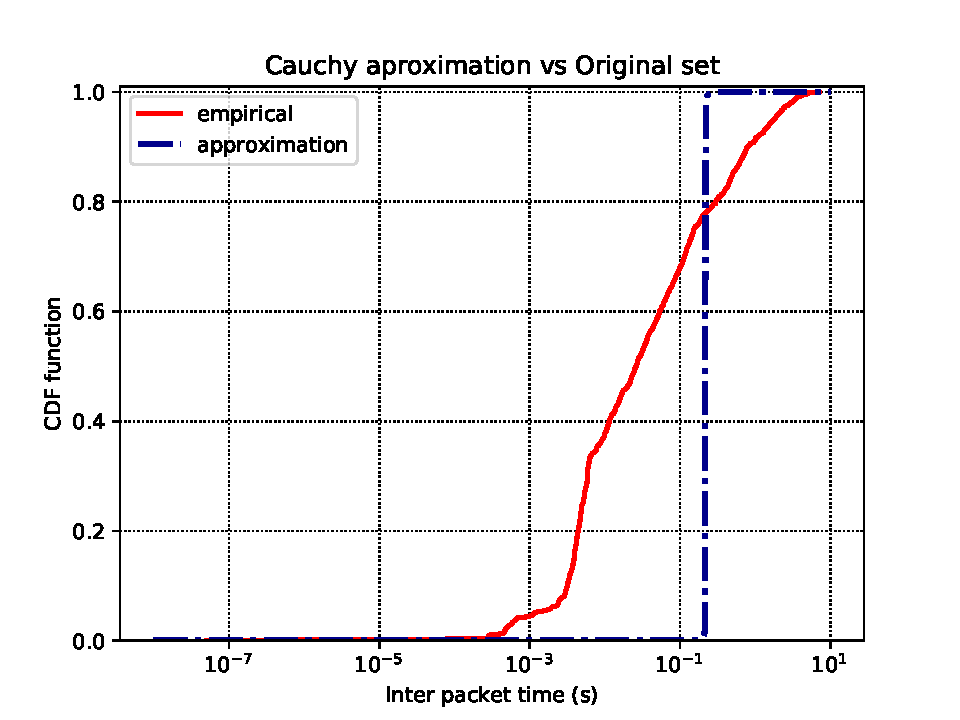
\includegraphics[width=62mm]{figures/ch4/Skype_Log_-_Cauchy_aproximation_vs_Original_set}
}
\subfloat[Exponential(LR)]{
  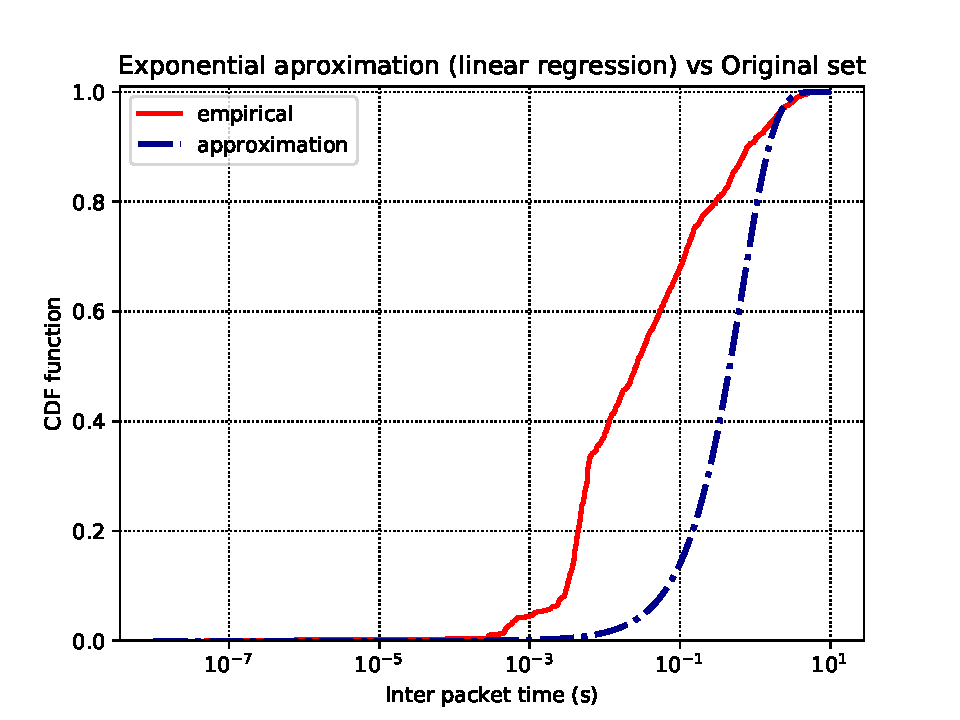
\includegraphics[width=62mm]{figures/ch4/Skype_Log_-_Exponential_aproximation_(linear_regression)_vs_Original_set}
}
\hspace{0mm}
\subfloat[Exponential(Me)]{
  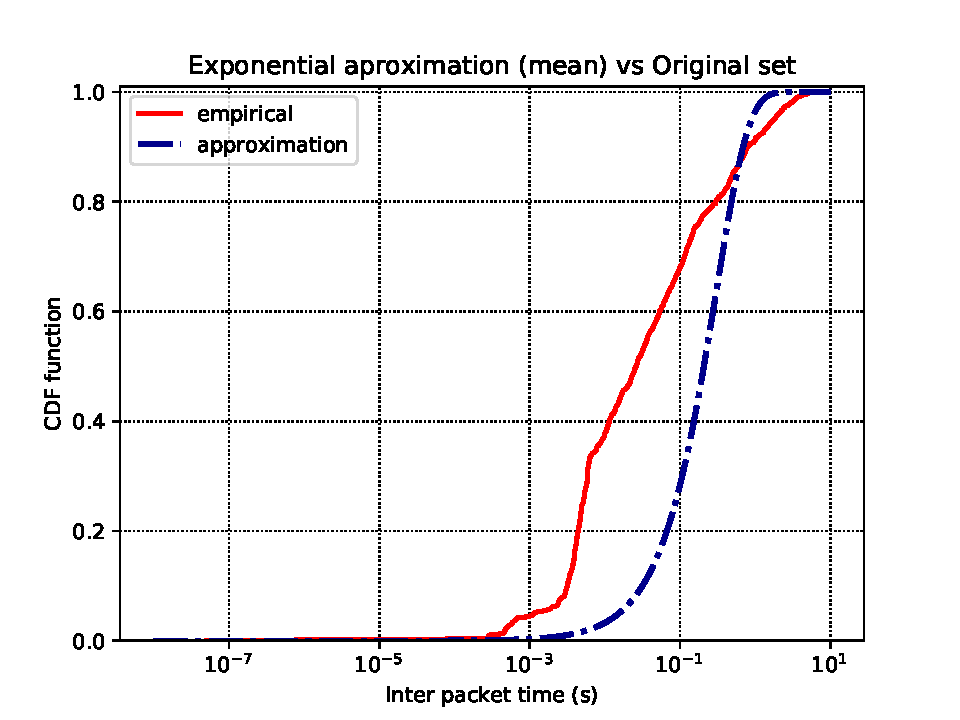
\includegraphics[width=62mm]{figures/ch4/Skype_Log_-_Exponential_aproximation_(mean)_vs_Original_set}
}
\subfloat[Normal]{
  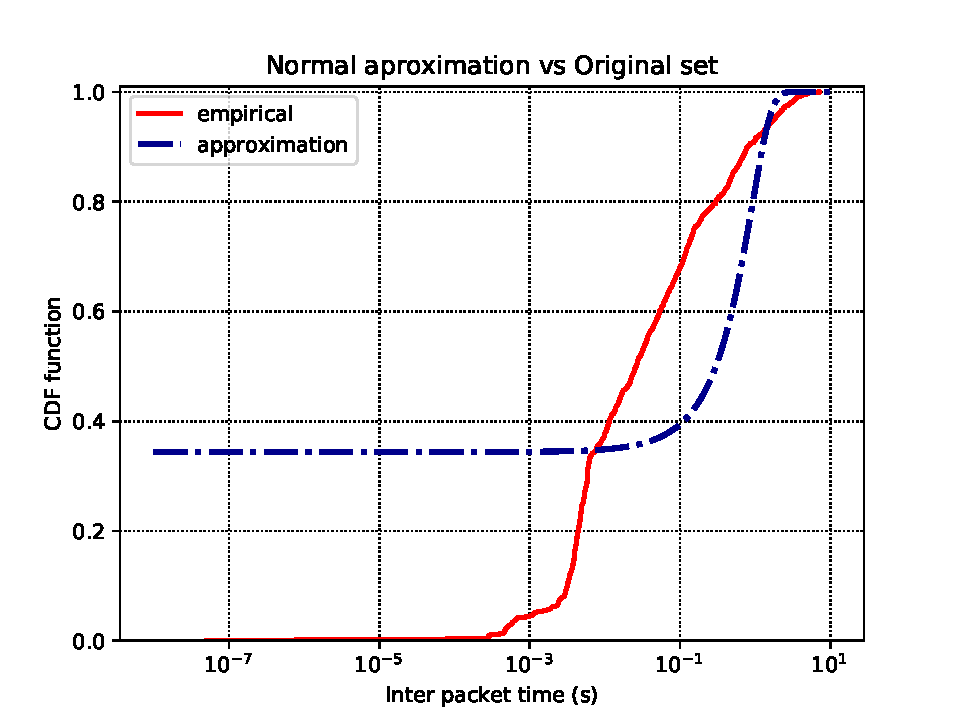
\includegraphics[width=62mm]{figures/ch4/Skype_Log_-_Normal_aproximation_vs_Original_set}
}
\hspace{0mm}
\subfloat[Pareto(LR)]{
  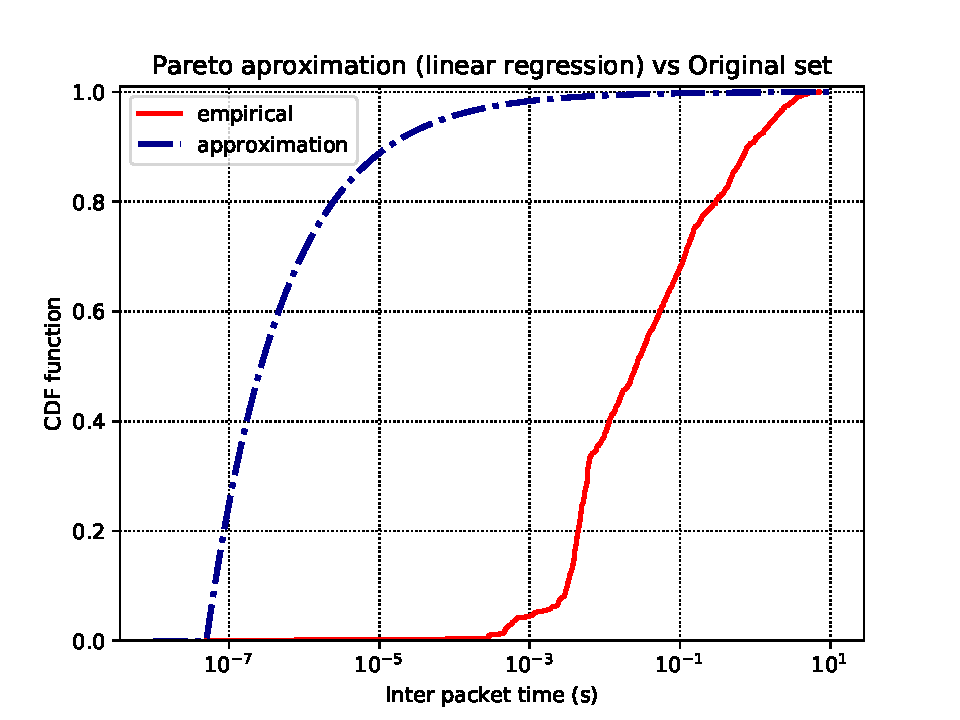
\includegraphics[width=62mm]{figures/ch4/Skype_Log_-_Pareto_aproximation_(linear_regression)_vs_Original_set}
}
\subfloat[Pareto(MLH)]{
  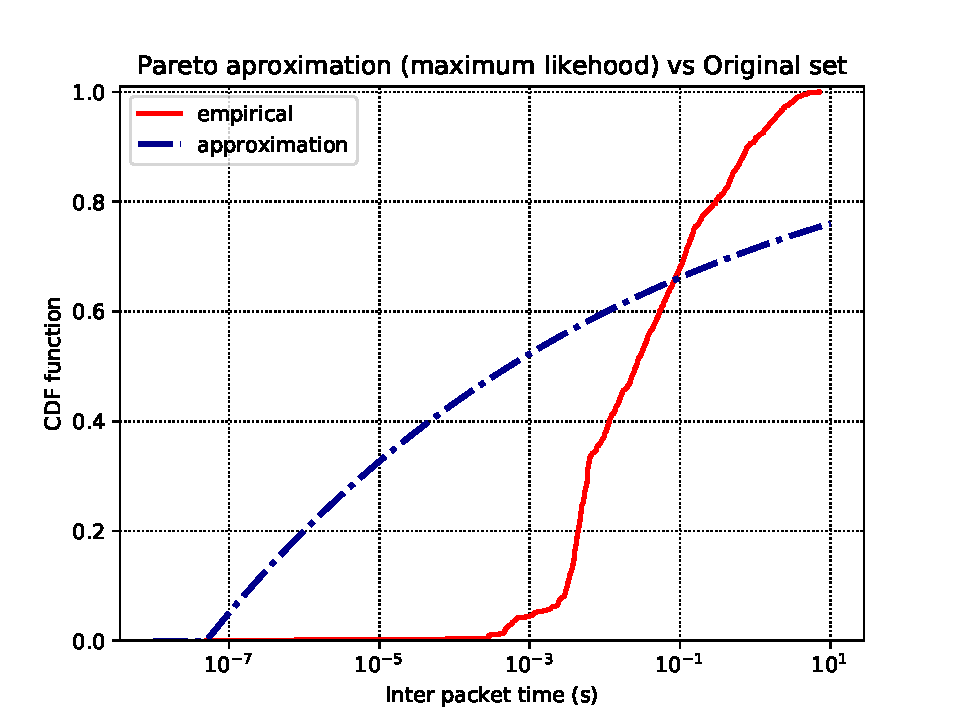
\includegraphics[width=62mm]{figures/ch4/Skype_Log_-_Pareto_aproximation_(maximum_likehood)_vs_Original_set}
}
\hspace{0mm}
\subfloat[Weibull]{
  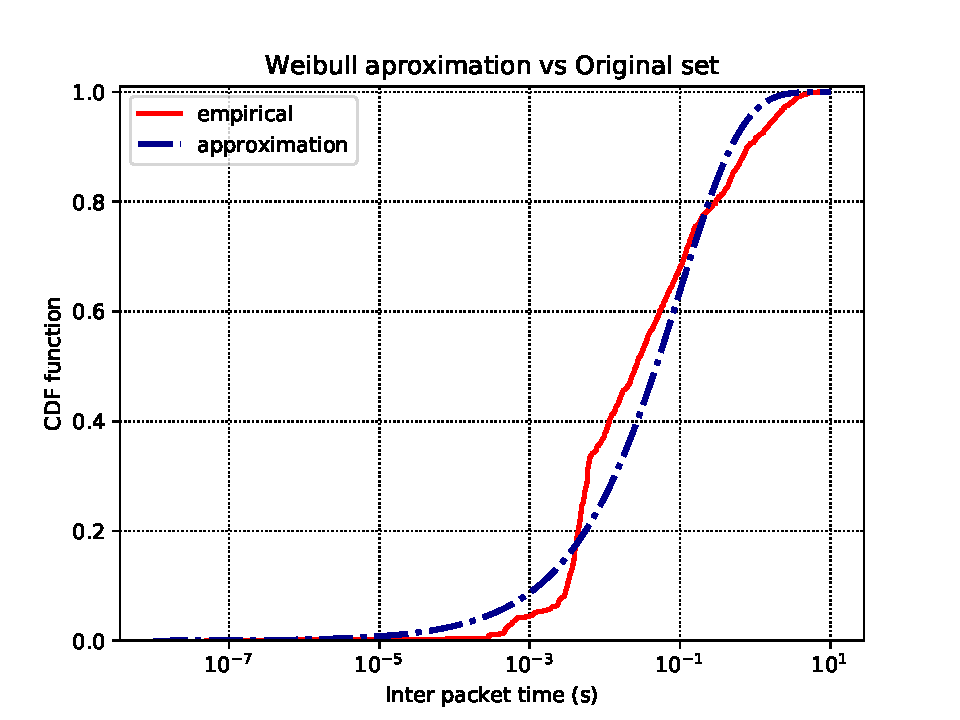
\includegraphics[width=62mm]{figures/ch4/Skype_Log_-_Weibull_aproximation_vs_Original_set}
}
\caption{CDF functions for the approximations of \textit{skype-pcap} inter  packet times, of many stochastic functions.}
\label{fig:aproximation-original-cdf}
\end{figure}


%%%%%%%%%%%%%%%%%%%%%%%
% QQplots Skype
%%%%%%%%%%%%%%%%%%%%%%%
\begin{figure}[pht!]
    \centering
    \subfloat[Chauchy]{
        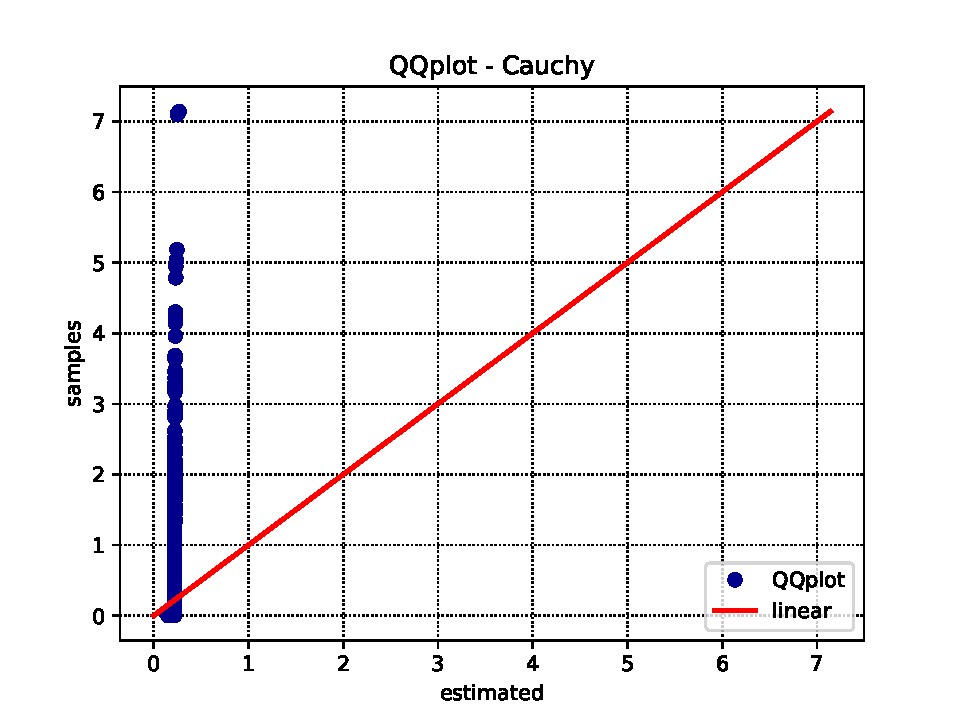
\includegraphics[width=62mm]{figures/ch4/Skype_QQplot_-_Cauchy}
    }
    \subfloat[Exponential(LR)]{
        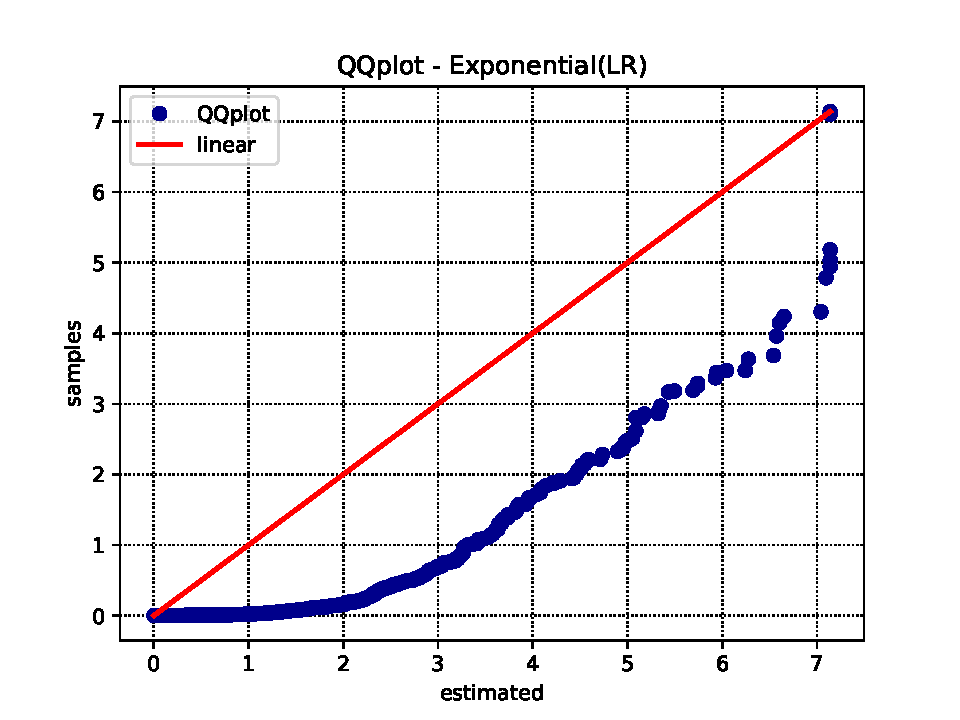
\includegraphics[width=62mm]{figures/ch4/Skype_QQplot_-_Exponential(LR)}
    }
    \hspace{0mm}
    \subfloat[Exponential(Me)]{
        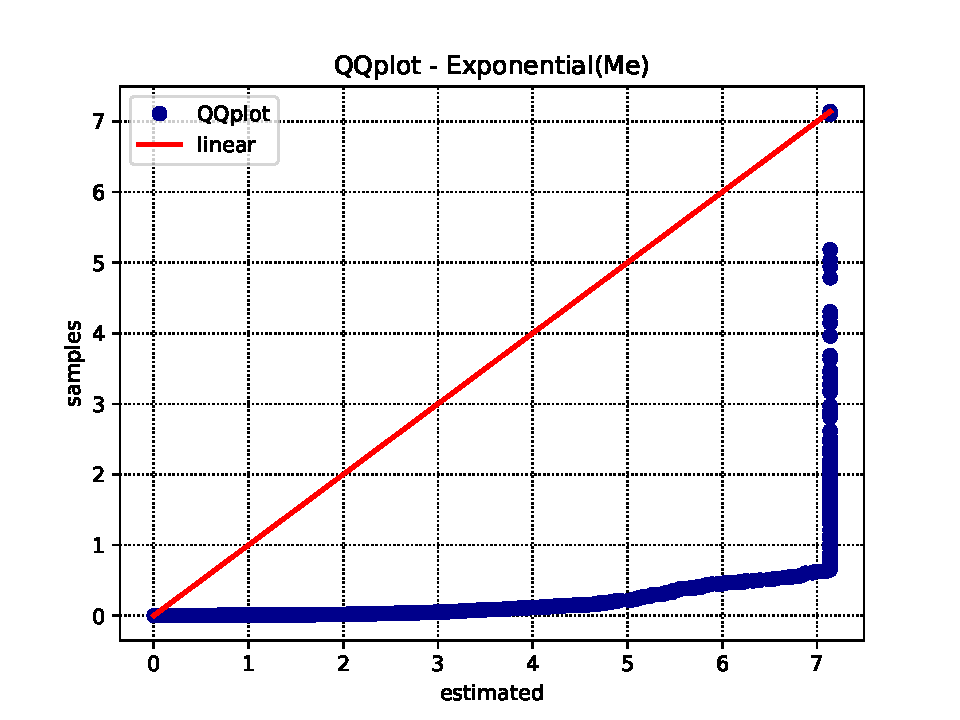
\includegraphics[width=62mm]{figures/ch4/Skype_QQplot_-_Exponential(Me)}
    }
    \subfloat[Normal]{
        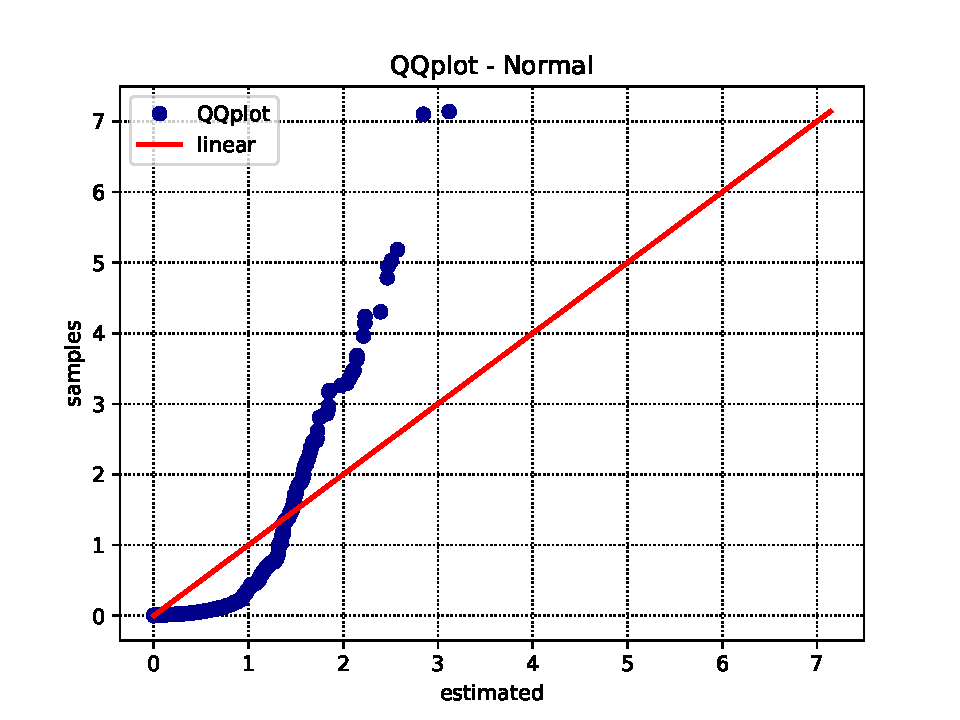
\includegraphics[width=62mm]{figures/ch4/Skype_QQplot_-_Normal}
    }
    \hspace{0mm}
    \subfloat[Pareto(LR)]{
        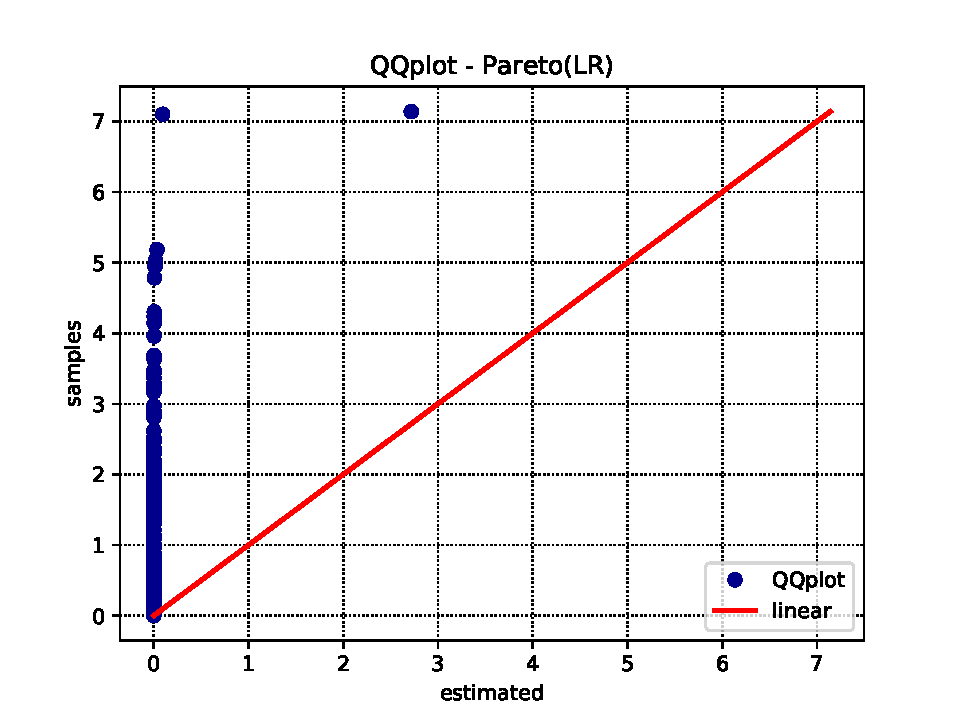
\includegraphics[width=62mm]{figures/ch4/Skype_QQplot_-_Pareto(LR)}
    }
    \subfloat[Pareto(MLH)]{
        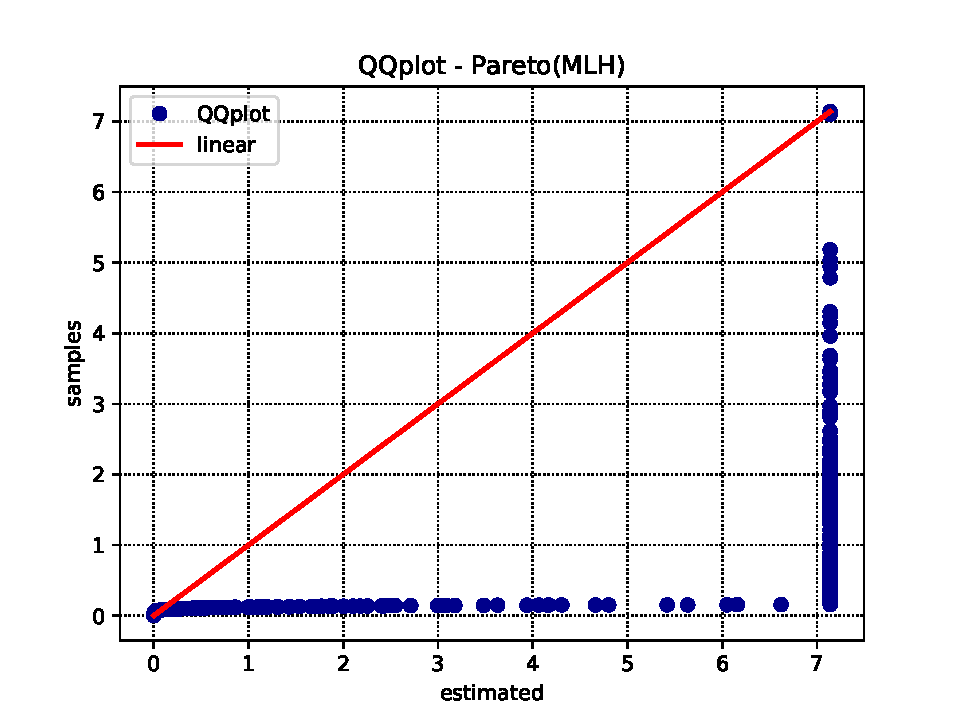
\includegraphics[width=62mm]{figures/ch4/Skype_QQplot_-_Pareto(MLH)}
    }
    \hspace{0mm}
    \subfloat[Weibull]{
        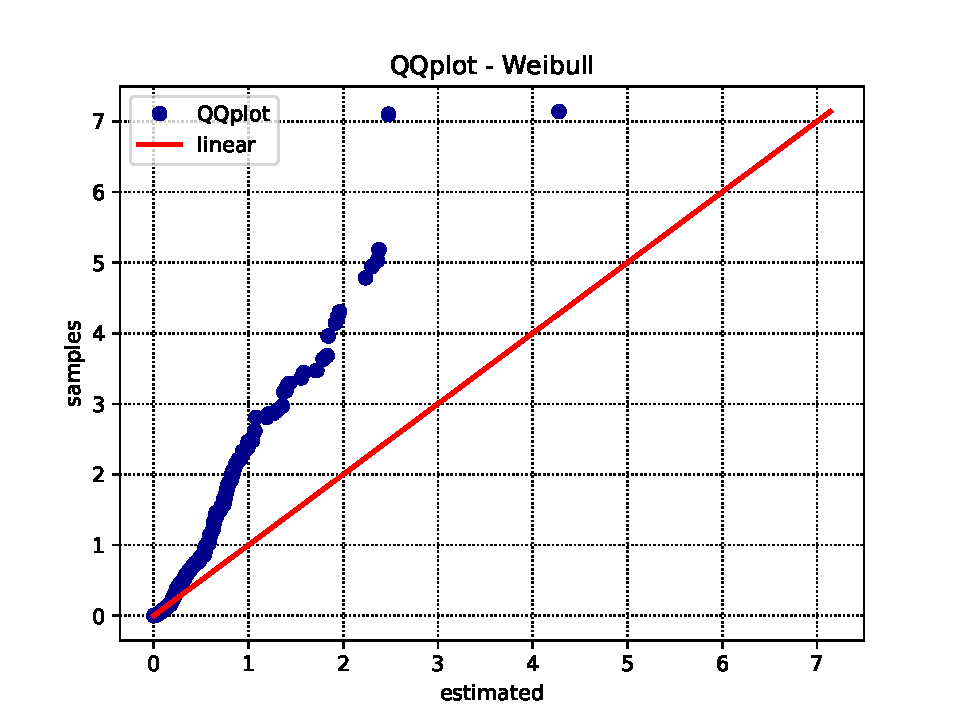
\includegraphics[width=62mm]{figures/ch4/Skype_QQplot_-_Weibull}
    }
    \caption{CDF functions for the approximations of \textit{skype-pcap} inter packet times, of many stochastic functions.}
    \label{fig:qq-skype}
\end{figure}


\begin{figure}[ph]
\centering
%%%%%%%%%%%%%%%%%%%%%%%
% Skype  - Correlation, Hurst, Mean Standard Deviation
%%%%%%%%%%%%%%%%%%%%%%%
\begin{figure}[H]
    \centering
    \subfloat[Correlation]{
        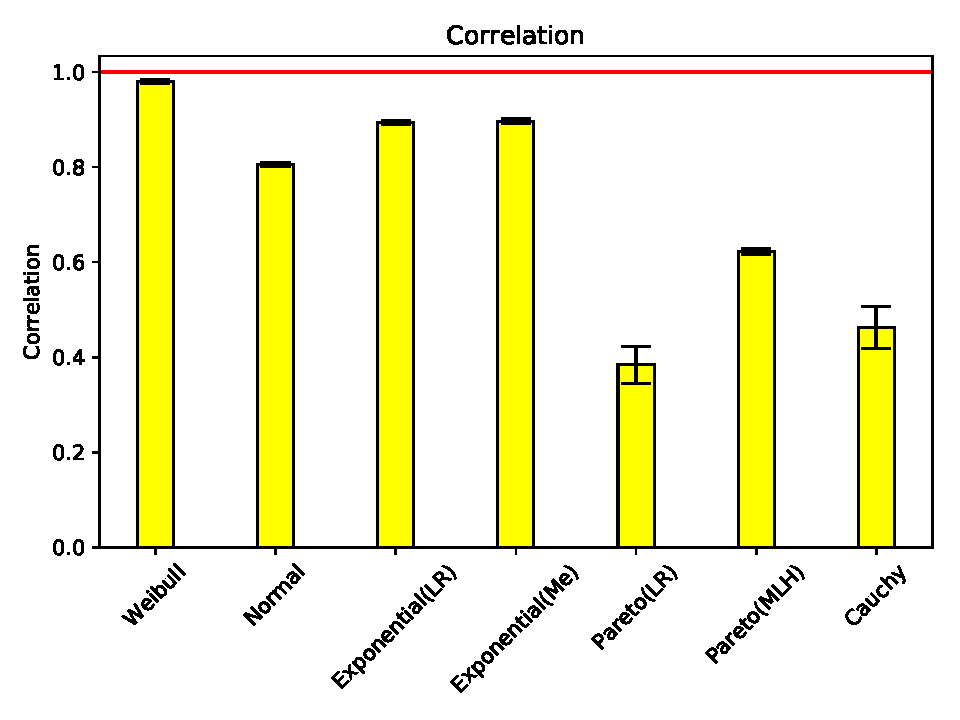
\includegraphics[width=60mm]{figures/ch4/Skype_Correlation}
        \label{correlation-skype}
    }
    \hspace{0mm}
    \subfloat[Hust Exponent]{
        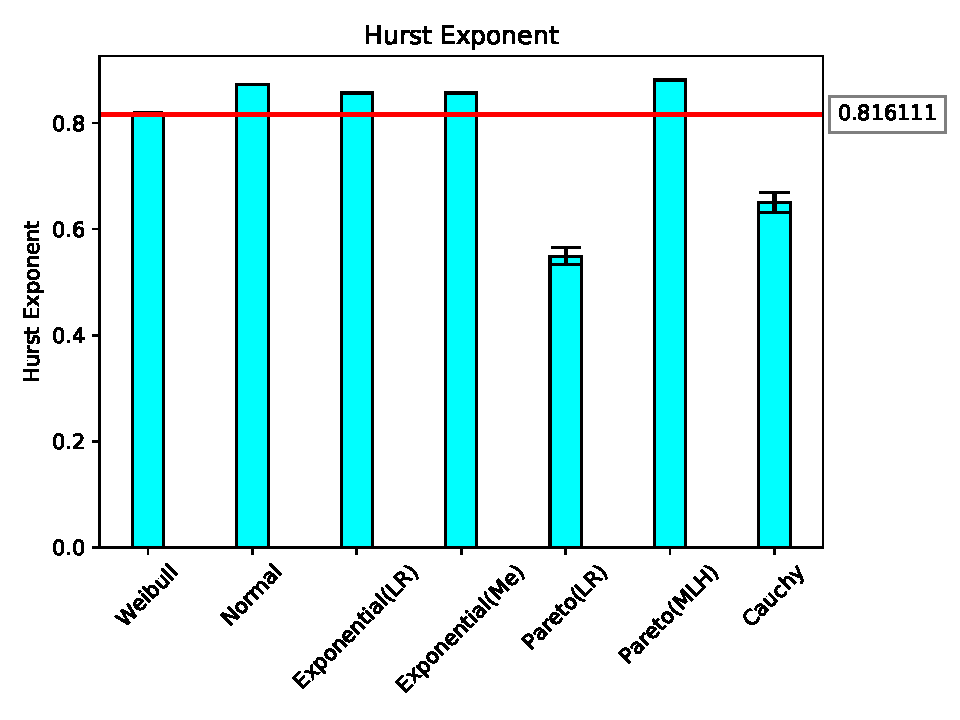
\includegraphics[width=60mm]{figures/ch4/Skype_Hurst_Exponent}
        \label{hurst-skype}
    }
    \hspace{0mm}
    \subfloat[Mean]{
        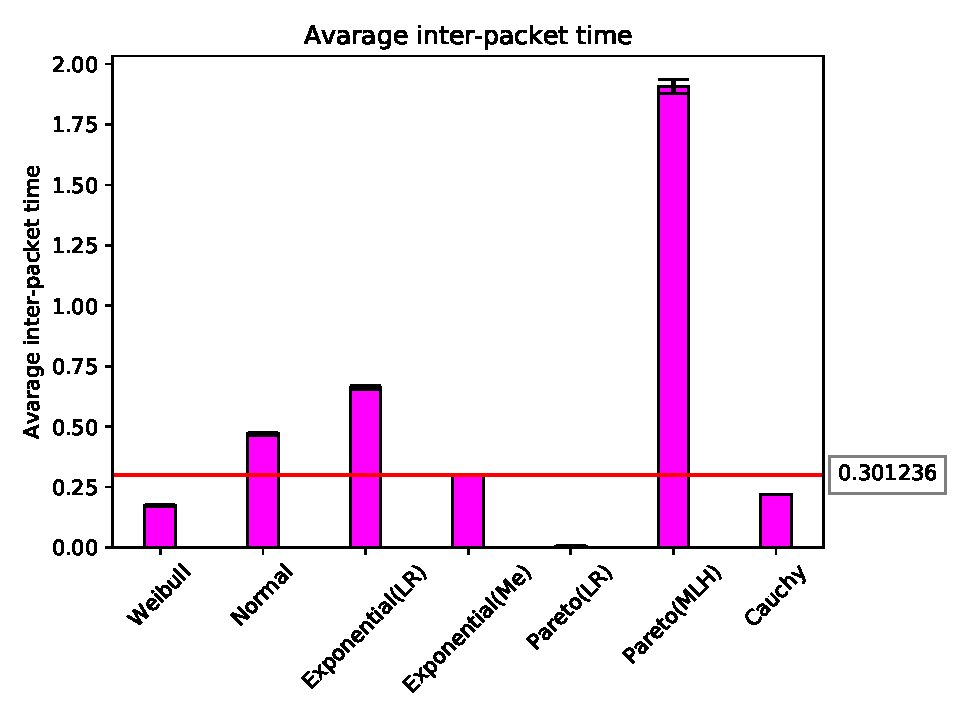
\includegraphics[width=60mm]{figures/ch4/Skype_Mean}
        \label{mean-skype}
    }
    \hspace{0mm}
    \subfloat[Standard Deviation]{
        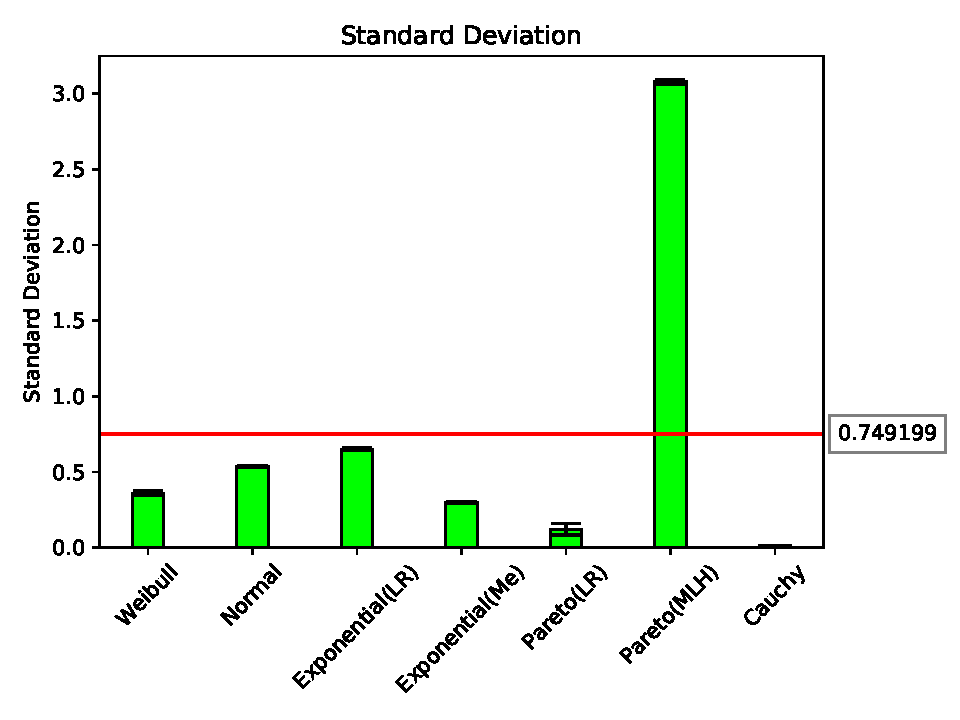
\includegraphics[width=60mm]{figures/ch4/Skype_Standard_Deviation}
        \label{std-skype}
    }
    \caption{Statistical parameters of \textit{skype-pcap} and its approximations}
    \label{fig:correlation-hurst-skype-pcap}
\end{figure}
%%%%%%%%%%%%%%%%%%%%%%%
% lan-gateway -  Correlation, Hurst, Mean Standard Deviation
%%%%%%%%%%%%%%%%%%%%%%%
\begin{figure}[H]
    \centering
    \subfloat[Correlation]{
        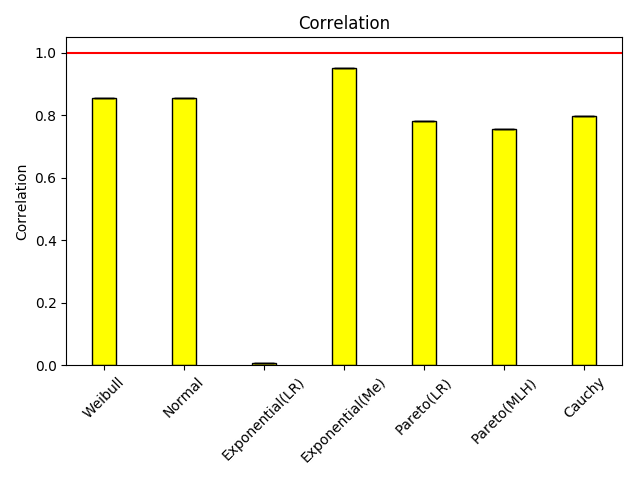
\includegraphics[width=60mm]{figures/ch4/bigFlows_Correlation}
        \label{lan-gateway-correlation-skype}
    }
    \hspace{0mm}
    \subfloat[Hust Exponent]{
        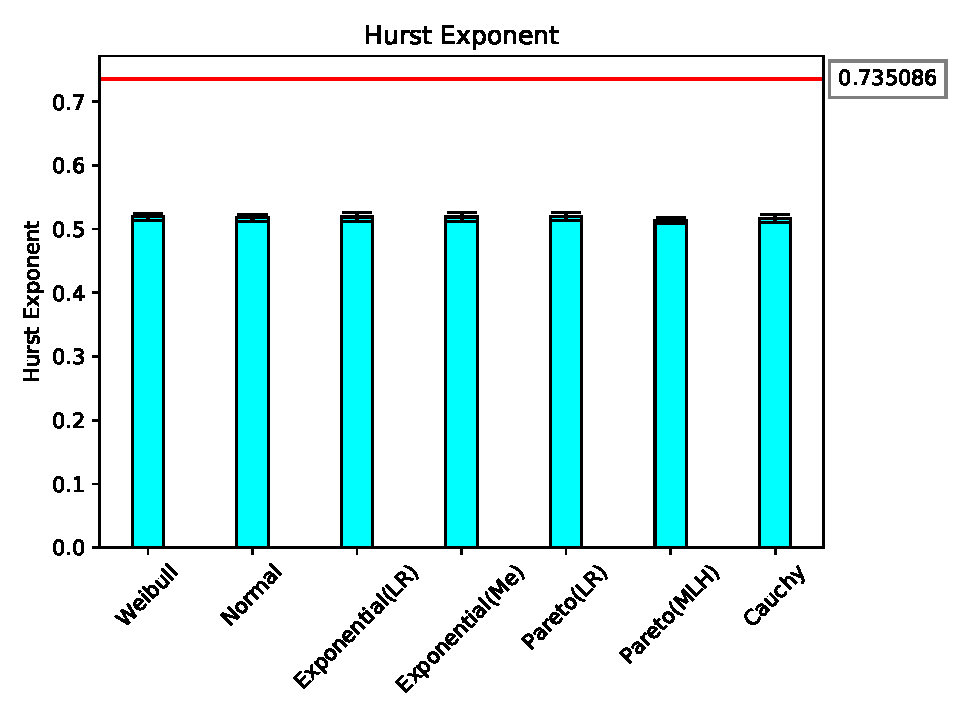
\includegraphics[width=60mm]{figures/ch4/bigFlows_Hurst_Exponent}
        \label{lan-gateway-hurst-skype}
    }
    \hspace{0mm}
    \subfloat[Mean]{
        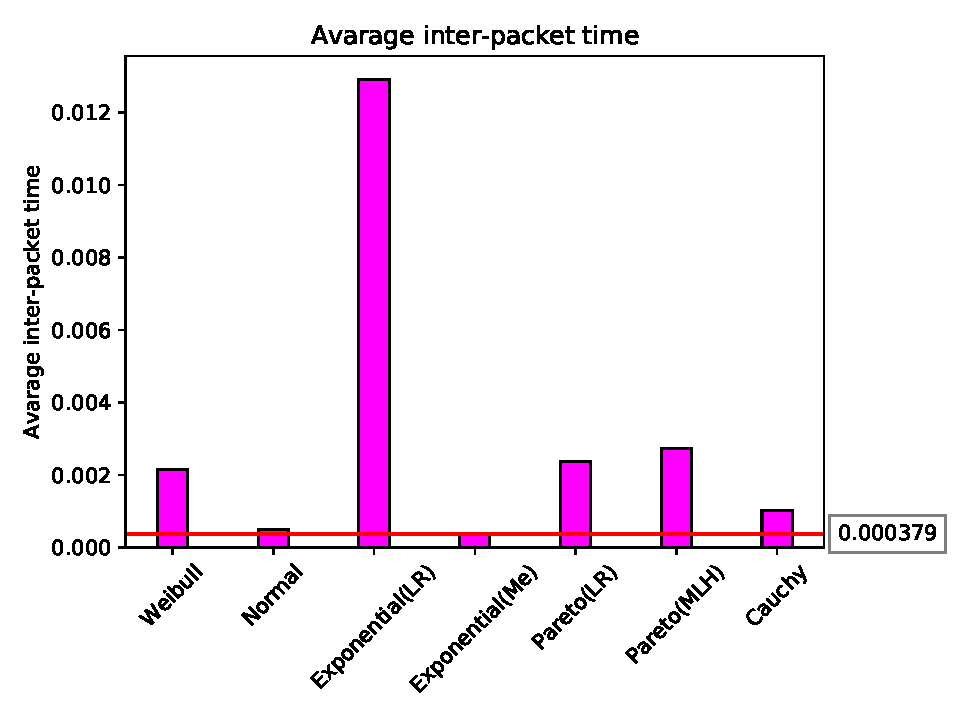
\includegraphics[width=60mm]{figures/ch4/bigFlows_Mean}
        \label{lan-gateway-mean-skype}
    }
    \hspace{0mm}
    \subfloat[Standard Deviation]{
        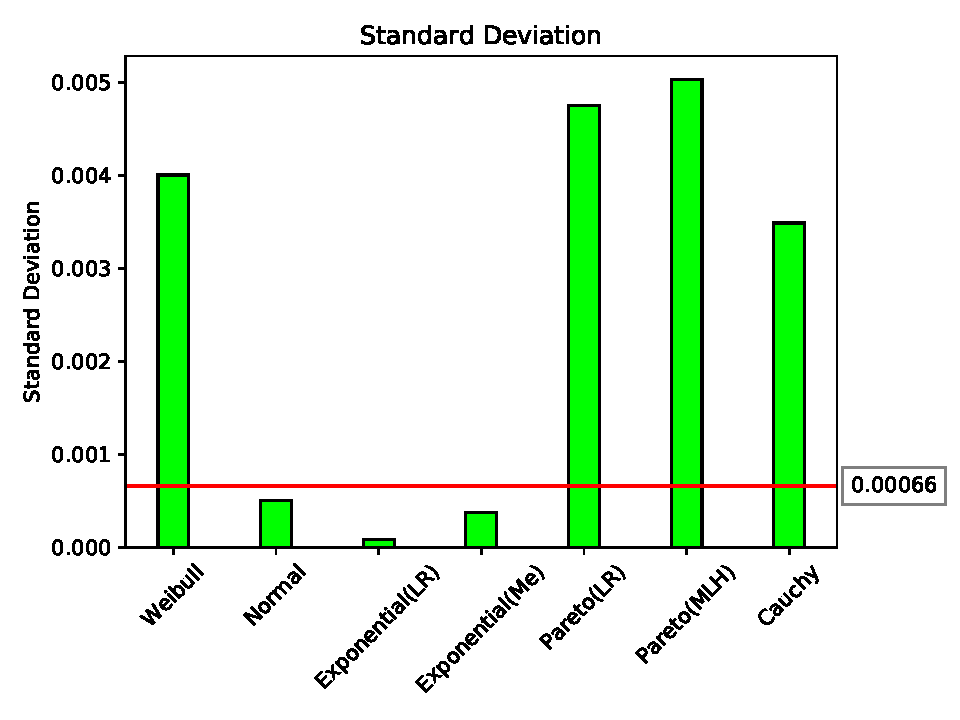
\includegraphics[width=60mm]{figures/ch4/bigFlows_Standard_Deviation}
        \label{lan-gateway-std-skype}
    }
    \caption{Statistical parameters of \textit{lan-gateway-pcap} and its approximations}
    \label{fig:correlation-hurst-lan-gateway-pcap}
\end{figure}
\end{figure}

\begin{figure}[ph]
%%%%%%%%%%%%%%%%%%%%%%%
% lanDirunal  - correlation, Hurst, Mean Standard Deviation
%%%%%%%%%%%%%%%%%%%%%%%
\begin{figure}[H]
    \centering
    \subfloat[Correlation]{
        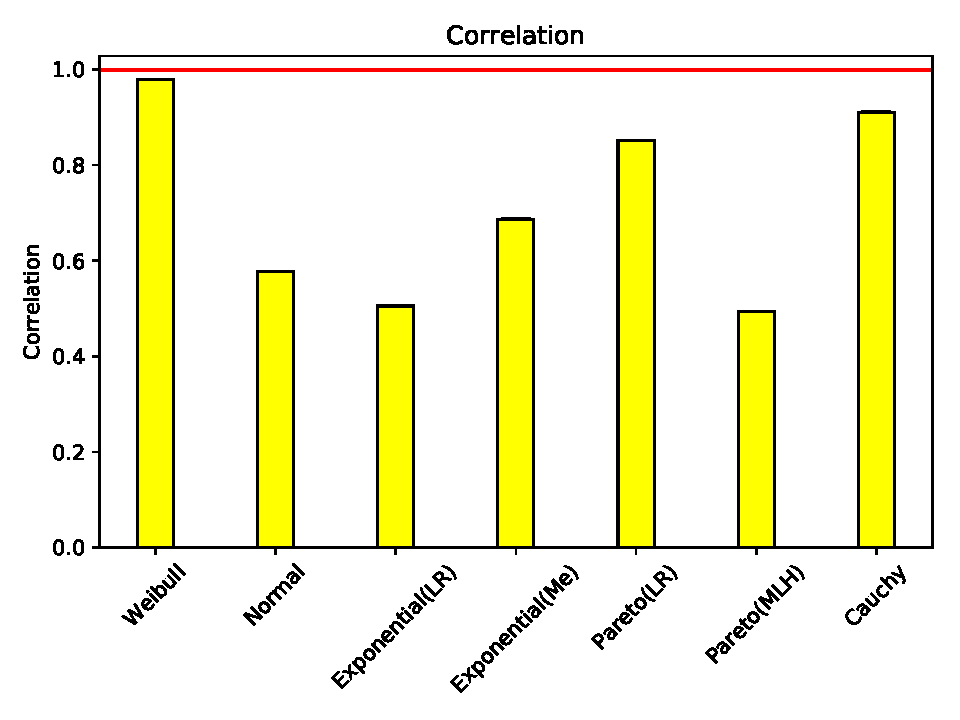
\includegraphics[width=60mm]{figures/ch4/Lan_Correlation}
        \label{Lan-correlation-skype}
    }
    \hspace{0mm}
    \subfloat[Hust Exponent]{
        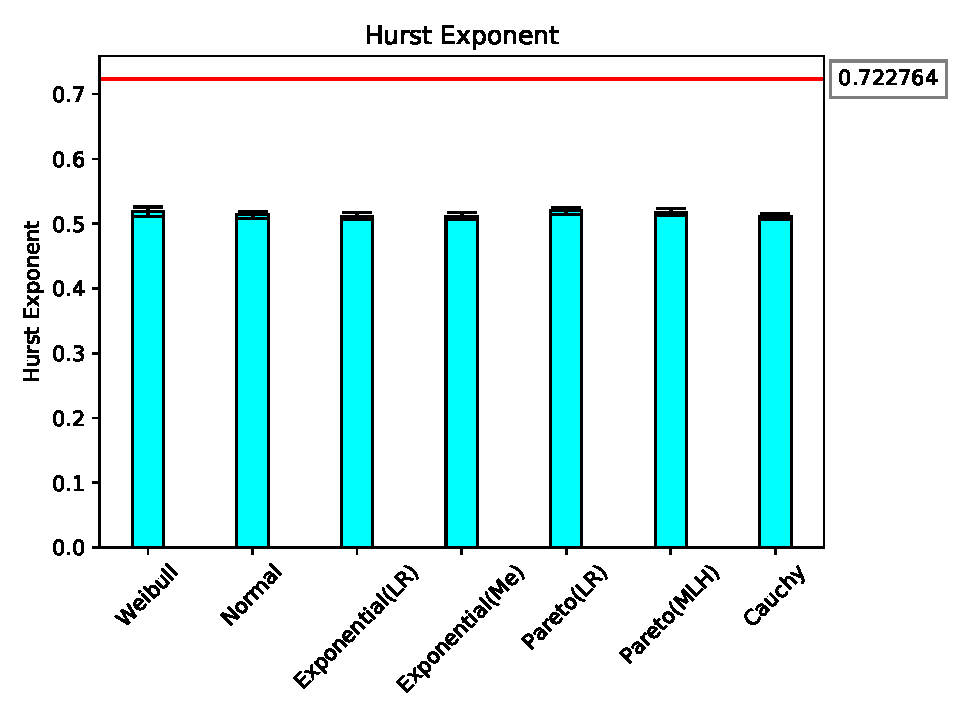
\includegraphics[width=60mm]{figures/ch4/Lan_Hurst_Exponent}
        \label{Lan-hurst-skype}
    }
    \hspace{0mm}
    \subfloat[Mean]{
        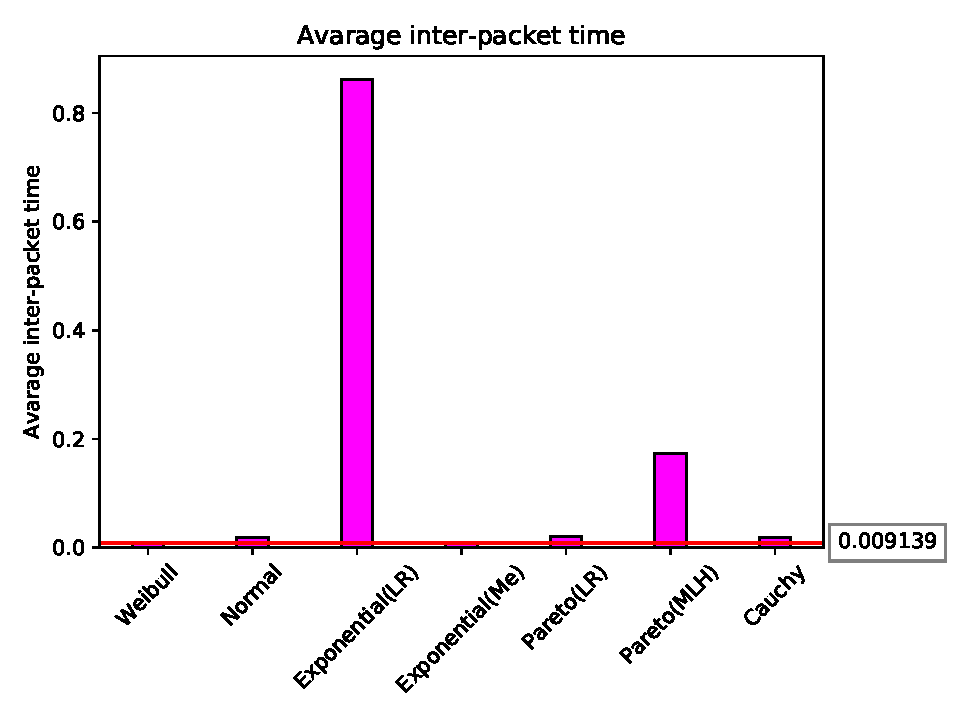
\includegraphics[width=60mm]{figures/ch4/Lan_Mean}
        \label{Lan-mean-skype}
    }
    \hspace{0mm}
    \subfloat[Standard Deviation]{
        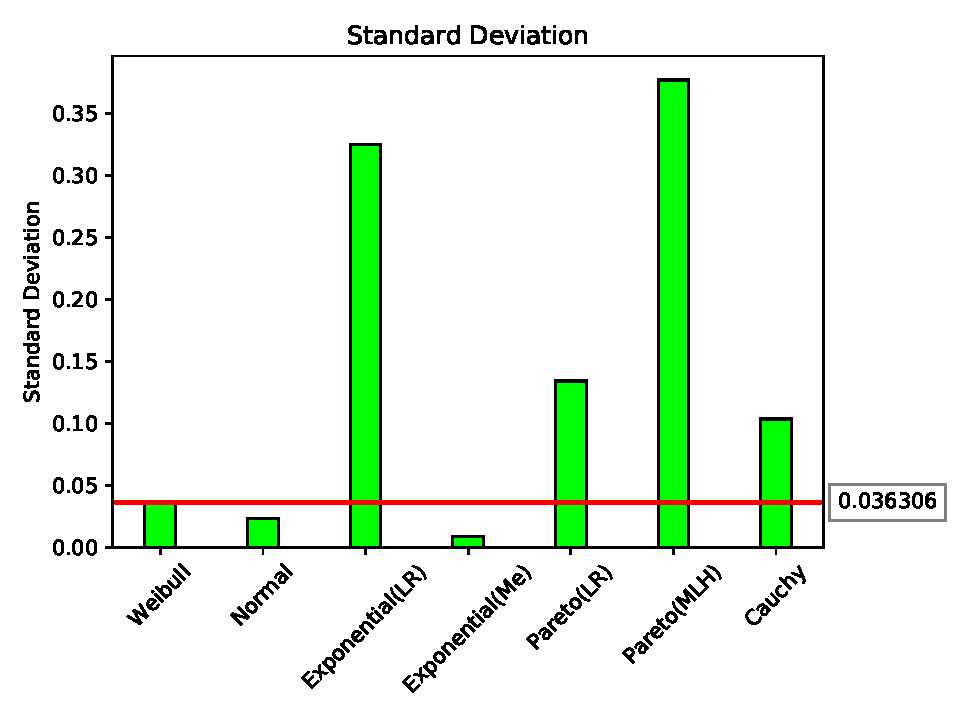
\includegraphics[width=60mm]{figures/ch4/Lan_Standard_Deviation}
        \label{Lan-std-skype}
    }
    \caption{Statistical parameters of \textit{lan-firewall-pcap} and its approximations}
    \label{fig:correlation-hurst-Lan-pcap}
\end{figure}
%%%%%%%%%%%%%%%%%%%%%%%
% Wan - correlation, Hurst, Mean Standard Deviation
%%%%%%%%%%%%%%%%%%%%%%%
\begin{figure}[H]
    \centering
    \subfloat[Correlation]{
        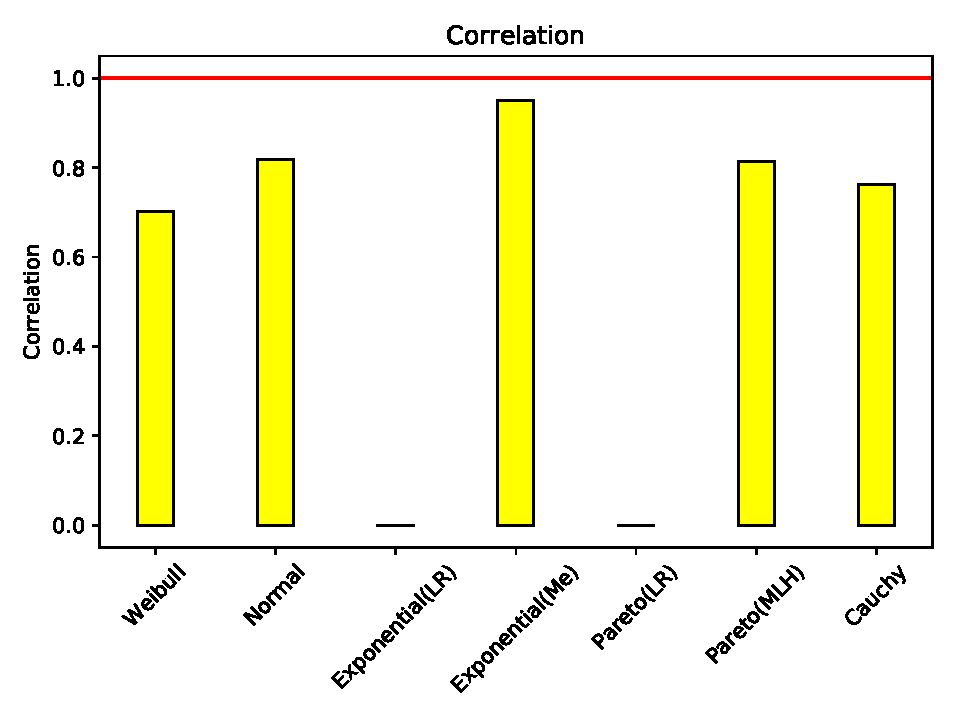
\includegraphics[width=60mm]{figures/ch4/Wan_Correlation}
        \label{Wan-correlation-skype}
    }
    \hspace{0mm}
    \subfloat[Hust Exponent]{
        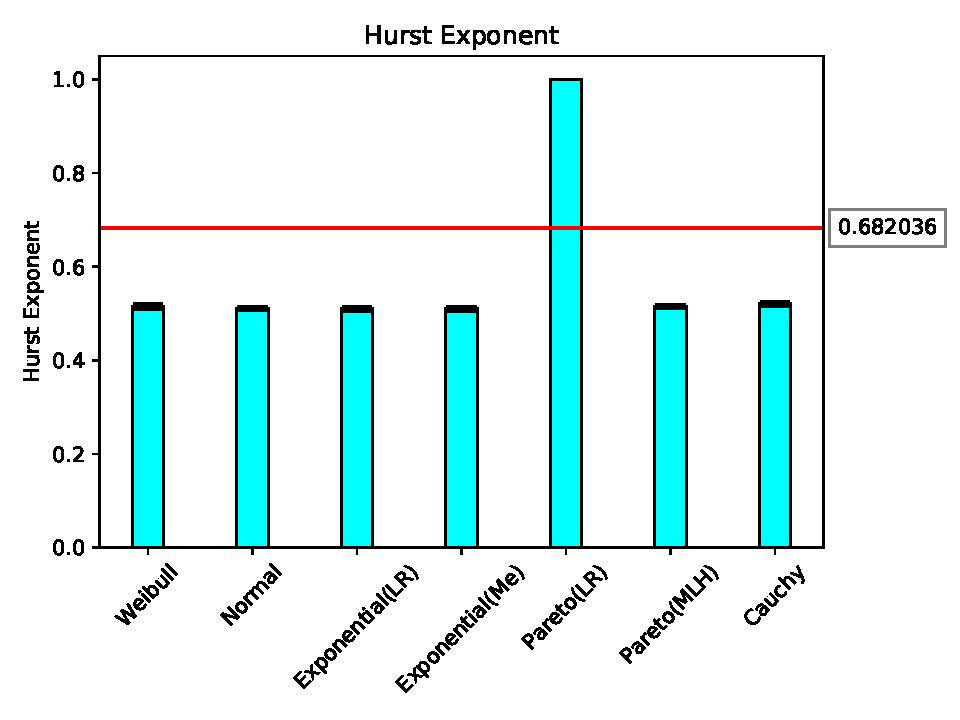
\includegraphics[width=60mm]{figures/ch4/Wan_Hurst_Exponent}
        \label{Wan-hurst-skype}
    }
    \hspace{0mm}
    \subfloat[Mean]{
        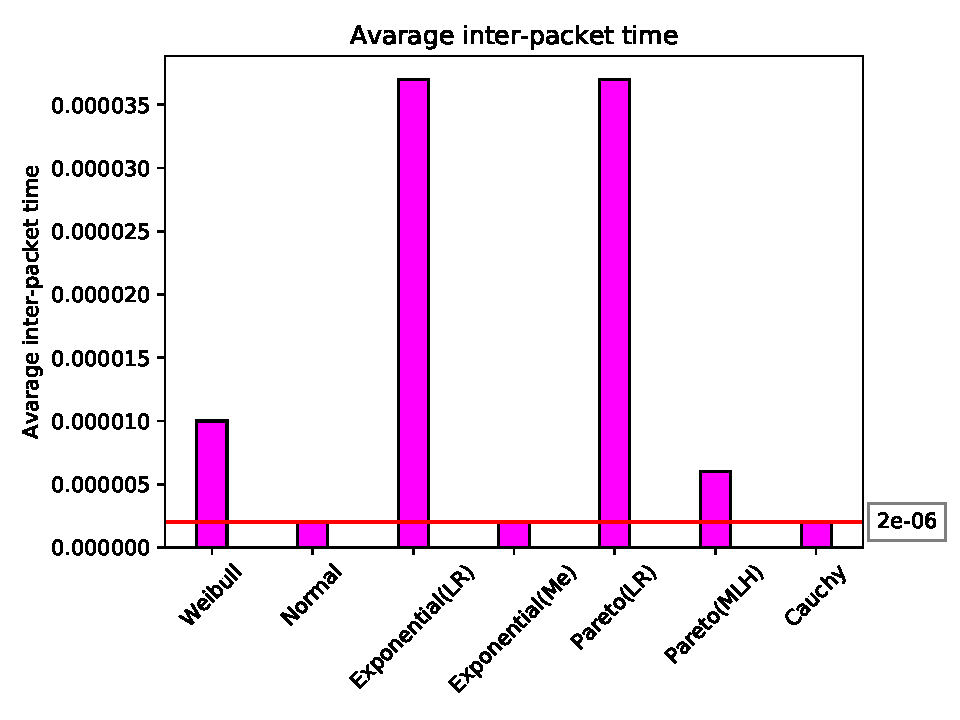
\includegraphics[width=60mm]{figures/ch4/Wan_Mean}
        \label{Wan-mean-skype}
    }
    \hspace{0mm}
    \subfloat[Standard Deviation]{
        \includegraphics[width=60mm]{figures/ch4/Wan_Standard_Deviation}
        \label{Wan-std-skype}
    }
    \caption{Statistical parameters of \textit{wan-pcap} and its approximations}
    \label{fig:correlation-hurst-wan-pcap}
\end{figure}
\end{figure}


\begin{figure}[ph]
%%%%%%%%%%%%%%%%%%%%%%%
% AIC BIC  diff
%%%%%%%%%%%%%%%%%%%%%%%
\begin{table}[H]
\centering
\caption{Relative difference(\%) between $AIC$ and $BIC$.}
\scalebox{0.90}{ 
\begin{tabular}{ccccc}
\hline
                & skype-pcap & \begin{tabular}[c]{@{}l@{}}lan-gateway\\ -pcap\end{tabular} & wan-pcap & \begin{tabular}[c]{@{}l@{}}lan-firewall\\ -pcap\end{tabular} \\ \hline
Weibull         & $7.47E-01$   & $3.96E-04$                                                    & $8.86E-05$ & $9.21E-04$                                                     \\
Normal          & $7.04E-01$   & $4.66E-04$                                                    & $7.58E-05$ & $NaN$                                                          \\
Exponential(LR) & $9.54E+00$   & $2.97E-04$                                                    & $4.26E-05$ & $2.81E-03$                                                     \\
Exponential(Me) & $2.00E+00$   & $2.00E-04$                                                    & $3.68E-05$ & $6.90E-04$                                                     \\
Pareto(LR)      & $2.53E-01$   & $4.25E-04$                                                    & $5.36E-05$ & $1.13E-03$                                                     \\
Pareto(MLH)     & $4.45E+00$   & $4.25E-04$                                                    & $7.74E-05$ & $1.04E-03$                                                     \\
Cauchy          & $1.23E-01$   & $5.97E-04$                                                    & $8.08E-05$ & $8.90E-03$                                                     \\ \hline
\end{tabular}
}
\label{tab:aic-bic-diff}
\end{table}
%%%%%%%%%%%%%%%%%%%%%%%
%validation Cost function
%%%%%%%%%%%%%%%%%%%%%%%
\begin{figure}[H]
    \centering
    \subfloat[\textit{skype-pcap}]{
        \includegraphics[width=62mm]{figures/ch4/Skype_costFunction}
        \label{cost-skype-pcap}
    }
    \hspace{0mm}
    \subfloat[\textit{lan-gateway-pcap}]{
        \includegraphics[width=62mm]{figures/ch4/bigFlows_costFunction}
        \label{cost-lan-gateway-pcap}
    }
    \hspace{0mm}
    \subfloat[\textit{lan-firewall-pcap}]{
        \includegraphics[width=62mm]{figures/ch4/Lan_costFunction}
        \label{cost-lan-pcap}
    }
    \hspace{0mm}
    \subfloat[\textit{wan-pcap}]{
        \includegraphics[width=62mm]{figures/ch4/Wan_costFunction}
        \label{cost-wan-pcap}
    }
    \caption{Cost function $J_M$ for each one of the data-sets used in this validation process}
    \label{fig:cost-function}
\end{figure}
\end{figure}

\begin{figure}[!ht]
%%%%%%%%%%%%%%%%%%%%%%%
% AIC / BIC order
%%%%%%%%%%%%%%%%%%%%%%%
\begin{figure}[H]
    \centering
    \includegraphics[scale=0.8]{figures/ch4/aic-bic-order.eps}
    \caption{Comparision of the quality order of each model given by $AIC$ and $BIC$}
    \label{fig:aic-bic-order}
\end{figure}
%%%%%%%%%%%%%%%%%%%%%%%
% Cost function order
%%%%%%%%%%%%%%%%%%%%%%%
\begin{figure}[H]
\centering
\includegraphics[scale=0.8]{figures/ch4/cost-function-summary.eps}
\caption{$J_M$ for each one of the datasets used in this validation process.}
\label{fig:model-order-cost}
\end{figure}
\end{figure}


\begin{figure}[!ht]
%%%%%%%%%%%%%%%%%%%%%%%
% CDFs eample
%%%%%%%%%%%%%%%%%%%%%%%
\begin{figure}[H]
\centering
\includegraphics[scale=0.7]{figures/ch4/cdfs}
\caption{Inter-packet times CDF function and stochastic models for \textit{firewall-pacap}.}
\label{fig:lan-firewall-cdf}
\end{figure}
%%%%%%%%%%%%%%%%%%%%%%%
% relative diff
%%%%%%%%%%%%%%%%%%%%%%%
\begin{figure}[H]
\centering
\includegraphics[scale=0.75]{figures/ch4/aicbic-costfunction-relative-diff}
\caption{Comparison of the model selection order for $BIC$/$AIC$ and  $J_M$ for each \textit{pcap}.}
\label{fig:cost-function_vs_aic-bic}
\end{figure}
\end{figure}


Here in this chapter we only discuss the approximation and QQplots achieved obtained by the \textit{pcap} \textit{skype-pcap}. All the other comments will be referent to the general results. The other fitting and QQ plots are provided on appendix~\ref{ap:aditional-plots} as a reference. 
We divided our analysis into 5 steps:
\begin{enumerate}
    \item \textit{CDF plots}
    \item \textit{QQplots}
    \item \textit{AIC} and \textit{BIC}
    \item \textit{Correlation, Hurst Exponent, Mean, and Standard Deviation} 
    \item  \textit{AIC} and \textit{BIC} vs. $\boldsymbol{J_M}$ 
\end{enumerate} 

\smallskip \noindent \textbf{\textit{CDF plots}}

Figure~\ref{fig:aproximation-original-cdf}  shows the CDF plots for \textit{skype-pcap}. They are on log-scale, which provide a better visualization for small time scales. 

\begin{itemize}
    \item We initially expected a good performance of heavy-tailed processes, but it depended on each case.
    \item Visually, the best result have seemed to be
    the Weibull trough linear regression, followed by Exponential(Me) -- what the $AIC$/$BIC$ analysis (figure~\ref{fig:aic-bic-order}) have confirmed. Also, Figure~\ref{fig:correlation-hurst-skype-pcap} show Weibull having the best Correlation and Hurst exponent, and the third best mean; while Exponential(Me) have had the best mean and the second best Correlation and Hurst exponent. 
    \item The Cauchy process have imposed an almost constant traffic, with the average inter-packet time close to the mean. Figure~\ref{fig:correlation-hurst-skype-pcap} confirms this observation since the process standard deviation is small, and the mean inter-packet time is close to the original (the second best);
    \item Exponential processes did not represented well small and larger values, compared to heavy-tailed processes, but were good to describe values closer to the average. On the other hand, a self-similar processes, such as Weibull and Pareto, have had a higher dispersion. The random-generated values were more wide-spared over the time -- what did not necessarily have implied on quality, as we are going to see. For example, Pareto(MLH) tended to over-estimate the amount of long values of inter-packet times, having a slower convergence of the CDF to one compared to the other processes -- about 20\% of the values are larger than 10 seconds. Cauchy for most of the case as a good process to represent the mean inter-packet times, but did no performed so well on other metrics (Figures      ~\ref{fig:correlation-hurst-wan-pcap}, ~\ref{fig:correlation-hurst-Lan-pcap}, ~\ref{fig:correlation-hurst-lan-gateway-pcap}, and  ~\ref{fig:correlation-hurst-skype-pcap})
    \item For the normal process, all values smaller than zero were zeroed, what have caused a vertical "off-set" on its CDF distribution. 
\end{itemize}

\smallskip  \noindent  \textbf{\textit{QQplots}}

On the QQplots(figure~\ref{fig:qq-skype}) we have observed that the original data had a much more influential heavy-tail effect when compared to the randomly generated on Cauchy, Exponential(Me), Pareto(LR), and Pareto(MLH) (appendix~\ref{ap:revision-probability}). We can observe  the The original data(samples) had a much influential heavy-tail effect compared to  the estimated data. We  verified this by the almost horizontal line made of blue dot-marks. On the other hand, Weibull process have had a much similar \textit{QQplot} compared to the samples.
Also we can identify a right-skew for Exponential(LR), Exponential(Me) and Pareto(MLH), and a left-skew for Cauchy, Pareto(LR) and Weibull.  On the other hand, the Normal distribution have presented a bi-modal behavior -- The first mode is on zero (since we zeroed all values smaller than zero), and the second, is close to the the average.


\smallskip \noindent  \textbf{\textit{AIC} and \textit{BIC}}

The calculated values for $AIC$, $BIC$, and processes parameters for all the traces are in table~\ref{tab:prototype-results}. We have verified in all cases  that the difference between $BIC$ and $AIC$ for a given process was always smaller compared to the difference between the values of a same criteria but among different processes to represent the same traffic. In another words, changing the criteria matter less than changing the process distribution. In our study,  $AIC$ and $BIC$ always have pointed to the same model ordering (figure ~\ref{fig:aic-bic-order}).

To compare these values of the information criteria, we calculated on the table  table~\ref{tab:aic-bic-diff} the relative difference between $AIC$ and $BIC$\footnote{ 
To calculate the relative difference $r_\%$ shown on table~\ref{tab:aic-bic-diff} we used this formula:
\begin{equation}
    r_\% = \frac{|V_1-V_2|}{\frac{(V_1+V_2)}{2}}\cdot100 
\end{equation}
}. The table indicate that the $AIC$ and $BIC$ converged to a common value as  the dataset size increasead\footnote{from the small to the larger dataset we have \textit{skype-pcap}, \textit{lan-gateway-pcap}, \textit{wan-pcap}, and \textit{lan-firewall-pcap}}. 
This result have indicated that, if the dataset is large enough, $AIC$ and $BIC$ will point to the same result. As table~\ref{tab:aic-bic-diff} shows, 9.54\% for Exponential(LR) was the larger difference between the information criteria. For the other pcaps, with a greater dataset, the differences were always small than 0.001\%. But, even the \textit{lan-firewall-pcap} being the largest one, the relative difference between its $AIC$ and $BIC$ is small than the ones form \textit{wan-pcap} and \textit{lan-gateway-pcap}. However, we have that information criteria depends on the likelihood value, and this on the individual probability of each value. We note that the standard deviation for packet times in \textit{lan-firewall-pcap} is considerably larger~\ref{fig:correlation-hurst-Lan-pcap}. This may be one of the possible causes for this observed behavior.



\smallskip \noindent  \textbf{\textit{Correlation, Hurst Exponent, Mean, and Standard Deviation}} 

In Figures ~\ref{fig:correlation-hurst-skype-pcap}, ~\ref{fig:correlation-hurst-lan-gateway-pcap}, and ~\ref{fig:correlation-hurst-wan-pcap}, and  ~\ref{fig:correlation-hurst-Lan-pcap} we show the results of properties calculated for each of the simulations of the stochastic processes: Correlation, Exponent of Hurst, Mean and Standard deviation. Each figure represents a different pcap file. The red horizontal line represents the value of the original traffic. Analyzing the quality of $AIC$ and $BIC$ on \textit{skype-pcap}, based on the figure results we see that concerning Correlation and Self-similarity it picked the right model: Weibull. Also regarding the average packet rate and dispersion, it is still one of the best choices. On regarding to the Mean, Exponential(Me) and Cauchy had the best performances. Regarding to the Standard Deviation, Exponential(Me) and Exponential(LR) had the best performance. Not by chance, Exponential(Me) $AIC$ and $BIC$ presented as the second best option. Comparing the results of the figures with the order suggested by AIC to BIC(Figure ~\ref{fig:aic-bic-order}), we noticed that the best ranked models showed a good performance in the metrics in general. We show the cost function $J_M$, able to summarize all the primary metrics in a single number, in figure~\ref{fig:cost-function}. All these results are abstracted by the cost function $J_M$. 


\smallskip \noindent  \textbf{\textit{AIC} and \textit{BIC} vs. $\boldsymbol{J_M}$ } 

Table~\ref{tab:prototype-results} summarizes the estimates obtained  for $AIC$, $BIC$, and the stochastic process estimated parameters for all \textit{pcap} traces. Each model order is graphically presented in Figure ~\ref{fig:aic-bic-order}.  For all \textit{pcap} experiments, we verify that the difference between $BIC$ and $AIC$ for a given function is always smaller than its value among different distributions. As shown in the table~\ref{tab:prototype-results}, $AIC$ and $BIC$ criteria always pointed to the same model ordering. Table~\ref{tab:aic-bic-diff} presents the percentage difference between the obtained values. We verify that their values tend to converge when the dataset increases. 

Figure~\ref{fig:cost-function} illustrates the cost function values for all the models on each \textit{pcap} file. For example, for \textit{skype-pcap}, $BIC$ and $AIC$ points that  Weibull and Exponential (Me) are the best representation for the traffic. The cost function used for cross-validation points both as best options, along with Exponential(LR).  To simplify the visualization and comparison of the differences between the rankings given by both methodologies, we created the plot~\ref{fig:cost-function_vs_aic-bic}.
The Figure~\ref{fig:cost-function_vs_aic-bic} presents a chart with the relative differences from the order of each model. Taking as a reference the position of each model given by $J$, we sorted them from the better to the worst (0 to 6, on the x-axis), and measured the position distance with the ones given by the information criteria. Since the worst case for this value is 6(opposite correspondence), we draw a line on the average: the expected value in the case no positive or negative correspondence existed between both information criteria and $J$. Using the $\phi$ operator, as defined before, we can calculate the ranking delta, as explained, for the \textit{i-th} model by:

\begin{equation}
\delta(m_i) = \phi(Jv, m_i) - \phi(IC, m_i)
\end{equation}

Where $Jv$ and $IC$ are the ordered pairs vectors on models and cost functions/information criteria, from the best to the worst, respectively.  We can observe that for mos to the use cases, the information criteria and the cost function had chosen models in a similar order. A hypothesis ranked well by one, tend to be ranked as good on the other. For the 28 possible study cases, 19 (68\%) had the same, or one-position difference on the ranking. 
Also, can point that $AIC$/$BIC$ tended to prioritize most of the heavy-tailed processes, such as Weibull and Pareto (except by Cauchy). It is a useful feature when the scaling and long-range characteristics of the traffic have to be prioritized by the selected model. 

Finally, we point out the $AIC$ and $BIC$ presented a bias in favor of Pareto(MLH). Even though it was never ranked as the best model, it was always better positioned by $AIC$ and $BIC$ than by $J$. We explain this result by the fact that $AIC$ and $BIC$ calculation uses the model likelihood, and the  Pareto(MLH) maximizes it.  This effect is clear on the \textit{lan-firewall-pcap}. On the figure~\ref{fig:lan-firewall-cdf} we plot the cross-validation dataset, the best fitting pointed by both methods (Weibull), and the second-best indicated by $J$ (Pareto(LR)) and by $AIC$/$BIC$(Pareto(MLH)). Even though Pareto(MLH) has a good performance representing small values, about 10\% of the inter-packet times are higher than 10 seconds, a prohibitive high value. It makes the Pareto(LR) overhaul performance better.


\subsection{Conclusion}


In this work, we introduce and evaluate a method based on $BIC$ and $AIC$ for analytic selection criteria of the best stochastic process to model network traffic. We use a cross-validation methodology based on random data generation following the selected models and cost function measurements. We observe that both $AIC$ or $BIC$ and the cost function were able to pick the first models in the same order, corroborating to our hypothesis of Akaike and Bayesian information criteria as reliable model selectors for network inter-packet times. We can conclude that $BIC$ and $AIC$ are suitable alternatives to derive realistic network traffic models for synthetic traffic generation. The only cave we point is on the use of the Maximum Likelihood method, that can over-prioritized some models over others with better performance. We summarize the implementation used on SIMITAR on algorithm~\ref{alg:stochasticModelFitting}.

%%%%%%%%%%%%%%%%%%%%%%%%%%%%%%%%%%%%%%%%%%%%%%%%%%%%%%%%%%%%%%%%%%%%%%%%%%%%%%%
%% ALGORITHM stochasticModelFitting
\begin{algorithm}[ht!]
    \caption{stochasticModelFitting}
    \label{alg:stochasticModelFitting}
    \begin{algorithmic}[1]
        \small        \Function{stochasticModelFitting}{$interArrivalData, criterion$}
        \State $m = interArrivalData.size$
        \State $interArrivalData = interArrivalData + MIN\_TIME$
        \If{$m < MINIMUM\_AMOUNT\_OF\_PACKETS$}
        \State $model\_list = \{constant\}$
        \Else
        \State $model\_list = \{weibull, pareto\_lr, pareto\_mlh, exponential\_me, exponential\_lr, normal,$
        \State $cauchy, constant\}$
        \EndIf
        
        \For{$model$ \textbf{in} $model\_list$}
        \State $model.fitting\_model(interArrivalData)$
        \EndFor
        \State $model\_list.sort(criterion)$
        \State \textbf{return} $model\_list$
        \EndFunction
    \end{algorithmic}
\end{algorithm}



\section{\texttt{calcOnOff}: an algorithm for estimating flow packet-train periods}


As we discussed in chapter~\ref{ch:architecture},  we developed an algorithm we call \texttt{calcOnOff}, listed on algorithm~\ref{alg:calcOnOff}. This procedure estimates the sizes of packet trains, as periods between packet trains in a flow context. 
This procedure receives as input values:

\begin{enumerate}
\item  \textbf{\texttt{arrivalTime}}: the list of packets arrivals on time on the flow. For example, if we have five packets arriving every two seconds, we would have: \texttt{arrivalTime = [0, 2, 4,  6, 8]};
\item  \texttt{deltaTime}: the list of inter-packet times on the flow. Following the same example presented before, we would have: \texttt{deltaTime = [2, 2, 2, 2]}. 
\item  \textbf{\texttt{cutTime}}: the time threshold that defines if we are still in the same train of packets, or a new one. 
\item  \textbf{\texttt{minOnTime}}: is the minimum length of flow ON time. minOnTime were used mainly to avoid ON times of zero seconds, in the case of only one packet, or when the time between packets is smaller than the operational system precision. 
\item  \textbf{\texttt{psSizeList}}: the list of packet sizes in bytes. 
\end{enumerate}


%%%%%%%%%%%%%%%%%%%%%%%%%%%%%%%%%%%%%%%%%%%%%%%%%%%%%%%%%%%%%%%%%%%%%%%%%%%%%%%
%% ALGORITHM CALC-ON-OFF
\begin{algorithm}[pt!]
    \caption{calcOnOff}
    \label{alg:calcOnOff}
    \begin{algorithmic}[1]
        \small
        \Function{calcOnOff}{$arrivalTime, deltaTime, cutTime, minOnTime$}%\Comment{Where A - array, p - left, q - middle, r - right}
        \State $m = deltaTime.length() - 1$
        \State $j = 0$
        \State $lastOff = 0$
        \State $pktCounterSum = 0$
        \State $fileSizeSum = 0$
        \For{$i = 0:m$}
        \State $pktCounterSum = pktCounterSum + 1$
        \State $fileSizeSum = fileSizeSum + psSizeList[i, 1]$
        \If{$deltaTime[i] > cutTime$} 
        \If{$i == 1$} \Comment{if the first is session-off time}
        \State $j++$
        \State $onTimes.push(minOnTime)$
        \State $offTimes.push(deltaTime[i])$
        \State $pktCounter.push(pktCounterSum)$
        \State $fileSize.push(fileSizeSum)$
        \State $pktCounterSum = 0$
        \State $fileSizeSum = 0$
        \Else \Comment{base case} 
        \State $pktCounter.push(pktCounterSum)$
        \State $fileSize.push(fileSizeSum)$
        \State $pktCounterSum = 0$
        \State $fileSizeSum = 0$
        \If{$j == 0$}
        \State $onTimes.push(arrivalTime[i - 1])$
        \State $offTimes.push(deltaTime[i])$
        \Else \Comment{others on times} 
        \State  $onTimes.push(max(deltaTime[i-1] - deltaTime[lastOff], minOnTime))$ 
        \State  $offTimes.push(deltaTime[i])$
        \EndIf
        \State $lastOff = i$
        \EndIf 
        \EndIf       
        \EndFor
        \State $pktCounterSum = pktCounterSum + 1$
        \State $fileSizeSum = fileSizeSum + psSizeList[m]$
        \If{$lastOff == m - 1$} \Comment{ if last is session-off }
        \State $onTimes.push(minOnTime)$ % on time
        \Else \Comment{ base last case}
        \If{$lastOff \neq 0$}
        \State $onTimes.push(arrivalTime[m] - arrivalTime[lastOff])$ 
        \Else 
        \State $onTimes.push(arrivalTime[m])$ \Comment{there was just on time}
        \EndIf
        \EndIf
        \State $pktCounter.push(pktCounterSum)$
        \State $fileSize.push(fileSizeSum)$
        \State \textbf{return} $onTimes, offTimes, pktCounter, fileSize$
        \EndFunction
    \end{algorithmic}
\end{algorithm}


For example, suppose a list of arrival times: 


\texttt{arrivalTime  = [0.0, 0.3  0.5, 0.6, 4.0, 4.3, 4.4 , 10.0] }

We would have the follow list of inter-packet times: 

\texttt{deltaTime = [0.3, 0.2, 0.1, 3.4,  0.3, 0.1, 5.6]}

Suppose the list of packet sizes is:

\texttt{psSizeList = [10, 20, 10, 30, 10, 40, 10, 50]}


With a \texttt{minOnTime} of 0.1 and a \texttt{cutTime} of 3 seconds, we would have the following output:

\texttt{onTimes = [0.6, 0.4, 0.1]}

\texttt{offTimes  = [3.4, 5.6]}

\texttt{pktCounter  = [4, 3, 1]}

\texttt{fileSize  = [70, 60, 50]}

Figure~\ref{fig:on-off} shows the same example, but with a text visualization, to simplify the visualization of the grouped data.

\begin{figure}
    \centering
    \includegraphics[width=\linewidth]{figures/ch4/on-off}
    \caption{Textual representation of the input and output data of calcOnOff.}
    \label{fig:on-off}
\end{figure}


\section{Typical header fields by Application protocols}


We also developed a simple test to guess the application protocol, based on the port numbers and the transport protocol used by each flow. If a flow matches the port number, and the transport protocol, it matches an application protocol, following the rules on table~\ref{tab:application-protocols}. 


\begin{table}[ht!]
    \centering
    \caption{Application match table}
    \label{tab:application-protocols}
    \begin{tabular}{lll}
        \hline
        Application Protocol & Transport Protocols & Transport Ports \\ \hline
        \acrshort{HTTPS}               & TCP                & 443             \\
        FTP                 & TCP                & 20, 21          \\
        HTTP                & TCP                & 80              \\
        \acrshort{BGP}                 & TCP                & 179             \\
        \acrshort{DHCP}                & UDP                & 67, 68          \\
        \acrshort{SNMP}                & UDP, TCP           & 161             \\
        \acrshort{DNS}                 & UDP, TCP           & 53              \\
        \acrshort{SSH}                 & UDP, TCP           & 22              \\
        Telnet              & UDP, TCP           & 23              \\
        \acrshort{TACACS}              & UDP, TCP           & 49              \\ \hline
    \end{tabular}
\end{table}


\section{Conclusions}


In this section, we explained on details methods mentioned in chapter~\ref{ch:architecture}. 
In this first section,  we revisited some classical works on modeling inter-packet times and packet trains. 

On the second we proposed the use of information criteria ($AIC$ and $BIC$) as tools for automatic selection of stochastic processes for inter-packet times. Since information criteria have not been tested for our study-case yet, were never tested for our study case, we developed an independent cross-validation method, based on traditional metrics for traffic validation. Since both procedures have converged to similar results, we conclude that $AIC$ and $BIC$ are reliable tools. However, we have to pay attention to processes parameterized the maximum likelihood method, since they tend to be prioritized, even performing poorly.  We abstracted this method for automatically select stochastic processes in algorithm~\ref{alg:stochasticModelFitting}. 

In the third and fourth section, we also present the methods used to estimate packet trains periods (algorithm~\ref{alg:calcOnOff}) and make the application classification (table~\ref{tab:application-protocols}). 

%\bookmarksetup{startatroot}%
%%%%%%%%%%%%%%%%%%%%%%%%%%%%%%%%%%%%%%%%%%%%%%%%%%%%%%%%%%%%%%%%%%%%%%%%%%%%%%%%
\chapter{Proof of Concepts}\label{ch:validation}
%%%%%%%%%%%%%%%%%%%%%%%%%%%%%%%%%%%%%%%%%%%%%%%%%%%%%%%%%%%%%%%%%%%%%%%%%%%%%%%%


%%%%%%%%%%%%%%%%%%%%%%%%%%%%%%%%%%%%%%%%%%%%%%%%%%%%%%%%%%%%%%%%%%%%%%%%%%%%%%%%'
\section{Testbed and Validation}


As the experimental platform for validation we use Mininet-based emulated scenarios.  For reproducibility purposes, Table~\ref{tab:specifications} presents all relevant experimental details. All the required scripts are available on the SIMITAR code repository\cite{projeto-github}. We use SIMITAR v0.4.2 (Eulemur rubriventer)\footnote{ We label the tags of SIMITAR control version on GitHub as lemurs species names (\href{https://en.wikipedia.org/wiki/List_of_lemur_species}{https://en.wikipedia.org/wiki/List\_of\_lemur\_species})}, as tagged at the GitHub repository. We explore a tree topology (Fig. ~\ref{fig:topo-tree}, and a one-hop connection (Fig.~\ref{fig:topo-simple}). Both scenarios as  SDN networks with an OpenDayLight (Beryllium) controller. We use two pcap files. The first is a Skype capture (\textit{skype-pcap}), and the second (\textit{lgw10s-pcap}) corresponds to the first ten seconds of a gateway capture\footnote{\textit{skype-pcap}: available at \url{https://wiki.wireshark.org/SampleCaptures}, named \textit{SkypeIRC.cap}; lgw10s-pcap avaiable at \url{http://tcpreplay.appneta.com/wiki/captures.html} named \textit{bigFlows.pcap}}. Host host \textit{h1} (IPv4 address 10.0.0.1) has generated the traffic, and was captured by TCPDump\footnote{TCPDump is a tool for monitoring and capturing network packets\cite{web-tcpdump}.} on \textit{pcap} format. 

To compare the degree of realism of the generated traffic, we use the flows' cumulative distribution function (CDF)\cite{harpoon-validation}, and the Wavelet multi-resolution analysis\cite{swing-paper}. On both analysis, the closer the plots are, the more realistic is the traffic generated by SIMITAR. The flow’s cumulative distribution measures the ingress of new flows over time, and it is a measure similarity and evolution of the traffic at the flow-level. On the other hand, the wavelet multi-resolution analysis can extract traffic scaling characteristics and is a measure of similarity at the packet-level. If the curve decreases, this indicates a periodicity on that time scale exists. If the curve remains approximately constant, it indicates similarity to white-noise. Finally, if the traffic has self-similar characteristics around a particular time scale, its curve increases linearly. Table~\ref{tab:results-summary} presents a compendium of metrics extracted from the traffic, including the Hurst exponent, which is a metric of the traffic fractal level. Self-similar  processes, such as the network traffic, have its value between 0.5  and 1.0 ($0.5 < H < 1.0 $)\cite{selfsimilar-ethernet}.


\begin{table}[!ht]
    \centering
    \caption{Experiments specification table}
    \label{tab:specifications}
    \begin{tabular}{ll}
        \hline
        Processor            & Intel(R) Core(TM) i7-4770, 8 cores, CPU @ 3.40GHz \\
        RAM                  & 15.5 GB                                           \\
        HD                   & 1000 GB                                           \\
        Linux         & 4.8.0-59-generic                                  \\
        Ubuntu        & Ubuntu 16.10 (yakkety)                            \\
        SIMITAR       & v0.4.2 (Eulemur rubriventer)                      \\
        Mininet       & 2.3.0d1                                           \\
        Iperf         & iperf version 2.0.9 (1 June 2016) pthreads        \\
        Libtins       & 3.4-2                                             \\
        OpenDayLight  & 0.4.0-Beryllium                                   \\
        Octave        & 4.0.3                                             \\
        Pyshark       & 0.3.6.2                                     \\
        Wireshark     & 2.2.6+g32dac6a-2ubuntu0.16.10               \\
        Tcudump       & 4.9.0 \\
        libpcap       & 1.7.4\\
        \hline
    \end{tabular}
\end{table}

\begin{figure}[!thb]
    \centering
    \includegraphics[width=\textwidth]{figures/ch5/topo-tree}
    \caption{Tree SDN topology emulated by mininet, and controlled by OpenDayLight Beryllium}
    \label{fig:topo-tree}
\end{figure}

\begin{figure}[!ht]
    \centering
    \includegraphics[width=0.8\textwidth]{figures/ch5/topo-simple}
    \caption{Single hop SDN topology emulated by mininet, and controlled by OpenDayLight Beryllium}
    \label{fig:topo-simple}
\end{figure}


\begin{table}[!htb]
	\centering
	\caption{Performed validations}
		\begin{tabular}{c c}
			\toprule
			\textbf{Metric Type} & \textbf{Validations} \\
			\midrule
			\makecell{Packet Based \\Metrics}                & \makecell{Data bit rate (kbps), Average packet\\
				rate (packets/s), Average packet size\\
				(bytes), Number of packets, Number of\\
				packets, Bandwidth over time}\\
			
			\makecell{Flow Based \\ Metrics}                & \makecell{Number of flows, Flows per second, \\
				Flows CDF distributions}\\
			
			\makecell{Fractal and Scaling \\ Characteristics} & \makecell{Hurst Exponent, Wavelet \\
				Multiresolution Analisis}\\
			\bottomrule
		\end{tabular}
	\label{tab:validation-tests-performed}
\end{table}


%%%%%%%%%%%%%%%%%%%%%%%%%%%%%%%%%%%%%%%%%%%%%%%%%%%%%%%%%%%%%%%%%%%%%%%%%%%%%%%%
\section{Results}


Figures ~\ref{fig:flows-cdf},~\ref{fig:wavelet} and Table~\ref{tab:results-summary} show the obtained results when comparing the original and the synthetic traffic generated by SIMITAR. We also illustrate the bandwidth traffic for one of the use cases in figure~\ref{fig:flows-bandwidth}. As we can see the generated traffics are not identical regarding bandwidth. However, both present similar fractal-like shape. The Hurst exponent of inter-packet times in every case has an error smaller than 10\% compared to the original in every case, i.e., the fractal-level of each synthetic traffic is indeed similar to the original trace.

The plot of flows per second seems much more accurate(~\ref{fig:flows-ps}), since most of the peaks match. Indeed, no visual lag between the plots. Even though the generated traffic is not identical to the original, the cumulative flow distribution obtained for every study-case is almost identical on every plot(figure~\ref{fig:flows-cdf}). The small differences on the curves result from threads and process concurrence for resources, in addition to noise from the sleep/wake processes on the thread signals. Since the operating system made the packet capture and timing, the packet capture buffer queue may have contributed as well. This result was our most significant achievement in our implementation. This result shows that our method of flow scheduling and independent traffic generation was effective and efficient in replicating the original traffic at the flow-level. However, the actual number of flows was more significant when SIMITAR used Iperf as the traffic generator API and slightly smaller when using libtins. This discrepancy can be explained because Iperf establishes additional connections to control the signaling and traffic statistics for every connection. On the other hand, with libtins, the number of flows is small, since a flow generation is aborted if the NetworkFlow flow class fails to create a new traffic flow. 

The results from the Wavelet multi-resolution analysis of inter-packet times vary in each case. The time resolution chosen was ten milliseconds, and it is represented in log 2 scale. The equation can calculate the time of each time-scale j: 

\begin{equation}
t = \frac{2^{j}}{100} [s]
\end{equation}

In the first case (figure ~\ref{fig:iperfCdf}), SIMITAR reproduced Skype traffic, using Iperf in a single-hop scenario. On small time scales, both curves increased linearly, which indicates a fractal shape. However, at this point, they exhibit different slopes with the synthetic traces behaving closer to a white-noise shape. After the time scales 5 and 6 (300-600 milliseconds) scale, the error between the curves becomes almost negligible. We also observe a periodicity pattern at the time-scale of 9 seconds. Vishwanath and Vahdat\cite{swing-paper}  measured the same periodicity pattern; which appears to be an intrinsic characteristic of  TCP traffic. We observe some periodicity at 11 and 13 time-scales (20 and 80 seconds). 

In the second case (Fig.~\ref{fig:iperftreeCdf}), on a tree topology on small time scales, we identify behavior closer to white-noise on small scales, and similar results, but with more substantial energy levels on greater time scales. The diversity introduced by the topology and the concurrent signaling traffic caused by the other hosts and switches does explain the observed behavior since node signaling tends to be more randomized than user-generated traffic. Indeed, as we can see in Table~\ref{tab:specifications}, there are two hundred more packets captured on the client interface in the tree topology compared to the one-hop scenario. 

In the last two plots (Figures~\ref{fig:tinsCdf} and ~\ref{fig:tinsLgwCdf}), where we use libtins as the packet crafter, the energy level is higher, and the curves are less correlated. SIMITAR, in the current implementation, is not modeling inter-packet with libtins and sends packets as fast as possible, which explains this discrepancy. However, in the last scenario, due to the higher average throughput, the observed performance was better.


\begin{table}[!htb]
    \centering
    \caption{Sumary of results comparing the original traces (italic) and te traffic generated by SIMITAR, with the description of the scenario.}
    \label{tab:results-summary}
    \scalebox{0.87}{
\begin{tabular}{lcccccc}
    \hline
    \multicolumn{1}{c}{\multirow{3}{*}{}} & \multirow{3}{*}{\textit{skype-pcap}} & \multicolumn{1}{c}{\multirow{3}{*}{\begin{tabular}[c]{@{}c@{}}skype, \\ one-hop, \\ iperf\end{tabular}}} & \multicolumn{1}{c}{\multirow{3}{*}{\begin{tabular}[c]{@{}c@{}}skype, \\ tree, \\ iperf\end{tabular}}} & \multicolumn{1}{c}{\multirow{3}{*}{\begin{tabular}[c]{@{}c@{}}skype, \\ one-hop, \\ libtins\end{tabular}}} & \multirow{3}{*}{\textit{lgw10s-pcap}} & \multicolumn{1}{c}{\multirow{3}{*}{\begin{tabular}[c]{@{}c@{}}lgw10s, \\ one-hop, \\ libtins\end{tabular}}} \\
    \multicolumn{1}{c}{}                  &                             & \multicolumn{1}{c}{}                                                                                     & \multicolumn{1}{c}{}                                                                                  & \multicolumn{1}{c}{}                                                                                       &                              & \multicolumn{1}{c}{}                                                                                        \\
    \multicolumn{1}{c}{}                  &                             & \multicolumn{1}{c}{}                                                                                     & \multicolumn{1}{c}{}                                                                                  & \multicolumn{1}{c}{}                                                                                       &                              & \multicolumn{1}{c}{}                                                                                        \\ \hline
    Hurst Exponent                        & 0.601                       & 0.618                                                                                                    & 0.598                                                                                                 & 0.691                                                                                                      & 0.723                        & 0.738                                                                                                       \\
    Data bit rate (kbps)                  & 7                           & 19                                                                                                       & 19                                                                                                    & 12                                                                                                         & 7252                         & 6790                                                                                                        \\
    Average packet rate (packets/s)       & 3                           & 4                                                                                                        & 5                                                                                                     & 6                                                                                                          & 2483                         & 2440                                                                                                        \\
    Average packet size (bytes)           & 260,89                      & 549,05                                                                                                   & 481,14                                                                                                & 224,68                                                                                                     & 365,00                       & 347,85                                                                                                      \\
    Number of packets                     & 1071                        & 1428                                                                                                     & 1604                                                                                                  & 2127                                                                                                       & 24 k                         & 24 k                                                                                                        \\
    Number of flows                       & 167                         & 350                                                                                                      & 325                                                                                                   & 162                                                                                                        & 3350                         & 3264                                                                                                        \\ \hline
\end{tabular}
    }
\end{table}


\begin{figure}[ph]
% Bandwidth
\begin{figure}[H]
    \centering
    \subfloat[\textit{Iperf, single-hop, skype-pcap}]{
        \includegraphics[width=72mm]{figures/ch5/skype-iperf-Bandwidth.pdf}
        \label{fig:iperfBw}
    }
    \hspace{0mm}
    \subfloat[\textit{Iperf, tree, skype-pcap}]{
        \includegraphics[width=72mm]{figures/ch5/skype-tree-iperf-Bandwidth.pdf}
        \label{fig:iperftreeBw}
    }
    \hspace{0mm}
    \subfloat[\textit{libtins, single-hop, skype-pcap}]{
        \includegraphics[width=72mm]{figures/ch5/skype-tins-Bandwidth.pdf}
        \label{fig:tinsBw}
    }
    \hspace{0mm}
    \subfloat[\textit{libtins, single-hop, langw10s-pcap}]{
        \includegraphics[width=72mm]{figures/ch5/lgw-tins-Bandwidth.pdf}
        \label{fig:tinsLgwBw}
    }
    \hspace{0mm}
    \caption{Traces bandwidth.}
    \label{fig:flows-bandwidth}
\end{figure}
% Flows per second
\begin{figure}[H]
    \centering
    \subfloat[\textit{Iperf, single-hop, skype-pcap}]{
        \includegraphics[width=72mm]{figures/ch5/skype-iperf-FlowsPs.pdf}
        \label{fig:iperfFps}
    }
    \hspace{0mm}
    \subfloat[\textit{Iperf, tree, skype-pcap}]{
        \includegraphics[width=72mm]{figures/ch5/skype-tree-iperf-FlowsPs.pdf}
        \label{fig:iperftreeFps}
    }
    \hspace{0mm}
    \subfloat[\textit{libtins, single-hop, skype-pcap}]{
        \includegraphics[width=72mm]{figures/ch5/skype-tins-FlowsPs.pdf}
        \label{fig:tinsFps}
    }
    \hspace{0mm}
    \subfloat[\textit{libtins, single-hop, langw10s-pcap}]{
        \includegraphics[width=72mm]{figures/ch5/lgw-tins-FlowsPs.pdf}
        \label{fig:tinsLgwFps}
    }
    \hspace{0mm}
    \caption{Flow per seconds}
    \label{fig:flows-ps}
\end{figure}
\end{figure}
\clearpage

\begin{figure}[ph]
% Flow CDF
\begin{figure}[H]
    \centering
    \subfloat[\textit{Iperf, single-hop, skype-pcap}]{
        \includegraphics[width=72mm]{figures/ch5/skype-iperf-FlowCdf.pdf}
        \label{fig:iperfCdf}
    }
    \hspace{0mm}
    \subfloat[\textit{Iperf, tree, skype-pcap}]{
        \includegraphics[width=72mm]{figures/ch5/skype-tree-iperf-FlowCdf.pdf}
        \label{fig:iperftreeCdf}
    }
    \hspace{0mm}
    \subfloat[\textit{libtins, single-hop, skype-pcap}]{
        \includegraphics[width=72mm]{figures/ch5/skype-tins-FlowCdf.pdf}
        \label{fig:tinsCdf}
    }
    \hspace{0mm}
    \subfloat[\textit{libtins, single-hop, langw10s-pcap}]{
        \includegraphics[width=72mm]{figures/ch5/lgw-tins-FlowCdf.pdf}
        \label{fig:tinsLgwCdf}
    }
    \hspace{0mm}
    \caption{Flows cumulative distributions.}
    \label{fig:flows-cdf}
\end{figure}
% Wavelet
\begin{figure}[H]
    \centering
    \subfloat[\textit{Iperf, single-hop, skype-pcap}]{
        \includegraphics[width=72mm]{figures/ch5/skype-iperf-WaveletMREA.pdf}
        \label{fig:iperfWaveletMREA}
    }
    \hspace{0mm}
    \subfloat[\textit{Iperf, tree, skype-pcap}]{
        \includegraphics[width=72mm]{figures/ch5/skype-tree-iperf-WaveletMREA.pdf}
        \label{fig:iperftreeWaveletMREA}
    }
    \hspace{0mm}
    \subfloat[\textit{libtins, single-hop, skype-pcap}]{
        \includegraphics[width=72mm]{figures/ch5/skype-tins-WaveletMREA.pdf}
        \label{fig:tinsWaveletMREA}
    }
    \hspace{0mm}
        \subfloat[\textit{libtins, single-hop, langw10s-pcap}]{
            \includegraphics[width=72mm]{figures/ch5/lgw-tins-WaveletMREA.pdf}
            \label{fig:tinsLgwWaveletMREA}
        }
        \hspace{0mm}
    \caption{Wavelet multiresolution energy analysis.}
    \label{fig:wavelet}
\end{figure}
\end{figure}
\clearpage


%%%%%%%%%%%%%%%%%%%%%%%%%%%%%%%%%%%%%%%%%%%%%%%%%%%%%%%%%%%%%%%%%%%%%%%%%%%%%%%%
\section{Conclusions}


We present SIMITAR as a tool and methodology to attend the evolving needs of rich and realistic network traffic experiments working at both flow-  and packet-level. At the flow-level, our methodology already achieves high fidelity results. The cumulative distribution of flows is almost identical in each case. From the perspective of benchmarking of a middle-boxes or SDN switches, this is a valuable result, since their performance, especially in SW implementations, largely depend on the number and characteristics of the stimuli flows. However, because of packets exchanged by background signaling connections, the traffic generated by Iperf, even following the same cumulative flow distribution, ended up creating more streams then expected.  

At the packet level, the current results with Iperf replicate with high accuracy the scaling characteristics of the first traffic, and the number of generated packets are not far than the expected.  Despite all identified optimization, the results are more than satisfactory and prove the potential of the proposed methodology. At the flow-level, our results are at least as good as those achieved by best-of-breed related work like Harpoon and Swing.  On the scaling characteristics, using lightweight traces, the results have been of comparable in quality.

%%%%%%%%%%%%%%%%%%%%%%%%%%%%%%%%%%%%%%%%%%%%%%%%%%%%%%%%%%%%%%%%%%%%%%%%%%%%%%%%
\chapter{Future Work}\label{ch:future-work}
%%%%%%%%%%%%%%%%%%%%%%%%%%%%%%%%%%%%%%%%%%%%%%%%%%%%%%%%%%%%%%%%%%%%%%%%%%%%%%%%

%%%%%%%%%%%%%%%%%%%%%%%%%%%%%%%%%%%%%%%%%%%%%%%%%%%%%%%%%%%%%%%%%%%%%%%%%%%%%%%
\section{Future Work's table}

On the table~\ref{tab:future-works} we list a set of ideas of future works. The sections A to D comprehends topics on the evolution of SIMITAR. Section E mentions new ideas of research that can contribute to SIMITAR evolution, but are not restricted to. Also, some topics can be a starting point for new tools.


\begin{table}[!ht]
\centering
\caption{Future Work's table}
\label{tab:future-works}
\begin{tabular}{lll}
\hline
\rowcolor[HTML]{9B9B9B} 
\multicolumn{1}{c}{\cellcolor[HTML]{9B9B9B}A} & \multicolumn{2}{l}{\cellcolor[HTML]{9B9B9B}Performance}                                                         \\ \hline
                                              & 1                          & Modeling Optimizations                                                             \\
                                              & \cellcolor[HTML]{EFEFEF}2  & \cellcolor[HTML]{EFEFEF}TinyFlows and flow merging                                 \\
                                              & 3                          & Smarter Flow Scheduler and thread management                                       \\
                                              & \cellcolor[HTML]{EFEFEF}4  & \cellcolor[HTML]{EFEFEF}DPDK KNI Interfaces                                        \\
                                              & 5                          & Multi-thread C++ Sniffer                                                           \\ \hline
\rowcolor[HTML]{9B9B9B} 
B                                             & \multicolumn{2}{l}{\cellcolor[HTML]{9B9B9B}Tool Support}                                                        \\ \hline
                                              & 1                          & Inter-packet times on TinsFlow                                                     \\
                                              & \cellcolor[HTML]{EFEFEF}2  & \cellcolor[HTML]{EFEFEF}D-ITG Flow Generator: DitgFlow                             \\
                                              & 3                          & DPDK Flow Generator: DpdkFlow                                                      \\
                                              & \cellcolor[HTML]{EFEFEF}4  & \cellcolor[HTML]{EFEFEF}Ostinato Flow Generator: OstinatoFlow                      \\
                                              & 5                          & ZigBee protocol Support                                                            \\ \hline
\rowcolor[HTML]{9B9B9B} 
C                                             & Calibration                &                                                                                    \\ \hline
                                              & 1                          & min\_time                                                                          \\
                                              & \cellcolor[HTML]{EFEFEF}2  & \cellcolor[HTML]{EFEFEF}min\_on\_time                                              \\
                                              & 3                          & session\_cut\_time                                                                 \\ \hline
\rowcolor[HTML]{9B9B9B} 
D                                             & \multicolumn{2}{l}{\cellcolor[HTML]{9B9B9B}New Components}                                                      \\ \hline
                                              & 1                          & Traffic Measurer                                                                      \\
                                              & \cellcolor[HTML]{EFEFEF}2  & \cellcolor[HTML]{EFEFEF}Pcap files crafter                                         \\
                                              & 3                          & Python/Lua Flow Generator                                                          \\ \hline
\rowcolor[HTML]{9B9B9B} 
E                                             & \multicolumn{2}{l}{\cellcolor[HTML]{9B9B9B}New Research Topics}                                                 \\ \hline
                                              & 1                          & Automated Selection of Inter-packet times models 2.0                               \\
                                              & \cellcolor[HTML]{EFEFEF}2  & \cellcolor[HTML]{EFEFEF}How how to craft malicious flows?                          \\
                                              & 3                          & Markovian-based traffic models                                \\
                                              & \cellcolor[HTML]{EFEFEF}4  & \cellcolor[HTML]{EFEFEF}Envelope-process based traffic models \\
                                              & 5                          & Relationship between Hurst and Hölder exponent, and stochastic processes.           \\
                                              & \cellcolor[HTML]{EFEFEF}6  & \cellcolor[HTML]{EFEFEF}Hurst-exponent feedbakc controll system for ON/OFF times   \\
                                              & 7                          & Traffic generation based on  Generative Adversarial Networks (GANs)  \\
                                              & \cellcolor[HTML]{EFEFEF}8  & \cellcolor[HTML]{EFEFEF} Realistic WAN, Wifi and IoT traffic \\
                                              & 9                          & SIMITAR vs Harpoon \\
                                              & \cellcolor[HTML]{EFEFEF}10 & \cellcolor[HTML]{EFEFEF}  How well traffic generators simulate reproduce stochastic processes?\\ 
                                              & 11                          & Traffic Generator Tools Survey \\
                                              \hline
\end{tabular}
\end{table}



%%%%%%%%%%%%%%%%%%%%%%%%%%%%%%%%%%%%%%%%%%%%%%%%%%%%%%%%%%%%%%%%%%%%%%%%%%%%%%%
\section{Performance}


\subsection{Modeling Optimizations}

\textbf{[A.1]} The primary issue of SIMITAR now is optimizing data processing for creating the Compact Trace Descriptor. The performance becomes an issue when processing large pcap files with more dozens of thousands of flows. The time expended for processing traces, in this case, is exceeding tens of hours. In the current implementation, the linear regression execution is mono-thread, and the stop criterion is just the number of iterations. Parallel processing, and creating stop criteria based on convergence in addition to the number of iterations will improve the performance, along with some code optimizations. Make the XML less verbose will help as well.

\subsection{TinyFlows and flow merging}

\textbf{[A.2]} Crating an option for merging flows is a possibility to improve the performance of traffic with several thousands of flows and Gigabits of bandwidth, such as from WAN captures. A merge criterion, for example, is to consider just network headers on flow’s classification. Also, the usage of simpler models for flows with a small number of packets (a "TinyFlow"), would improve the processing speed.

\subsection{Smarter Flow Scheduler and thread management}

\textbf{[A.3]} Currently, SIMITAR instantiates all the flow threads once the traffic generations start.  A smarter traffic generation where SIMITAR instantiates each thread when the traffic, and join when it is inactive should reduce the overhead for traces with a large number of flows. 

\subsection{DPDK KNI Interfaces}

\begin{figure}[!ht]
    \centering
    \includegraphics[height=2.0in]{figures/ch6/dpdk-interface.pdf}
    \caption{Usage of DPDK KNI interfaces.}
    \label{fig:dpdk-kni}
\end{figure}

\textbf{[A.4]} One possibility to improve the traffic generation performance issue DPDK Kernel NIC Interface (\acrshort{KNI} interfaces) 2. DPDK KNI interfaces allow applications from the user’s space to interact with DPDK ports. In this way, we may achieve a faster packet processing.

\subsection{Multi-thread C++ Sniffer}

\textbf{[A.5]} Implementing a C/C++ multi-thread sniffer will improve the processing time of packets. 



%%%%%%%%%%%%%%%%%%%%%%%%%%%%%%%%%%%%%%%%%%%%%%%%%%%%%%%%%%%%%%%%%%%%%%%%%%%%%%%
\section{Tool Support}

\subsection{Inter-packet times on TinsFlow}

\textbf{[B.1]} SIMITAR’s current implementation using libtins to generate the packets does not model inter-packet times. Modeling this feature will improve the scaling characteristics of libtins traffic.

\subsection{D-ITG, Ostinato and DPDK Flow Generators: DitgFlow, OstinatoFlow, DdpkFlow}

\begin{figure}[!ht]
    \centering
    \includegraphics[height=2.0in]{figures/ch6/dpdk-flow}
    \caption{DddkDlow and DitgFlow}
    \label{fig:dpdk-flow}
\end{figure}


\textbf{[B.2-4]} Expand SIMITAR to other traffic generator tools(figure~\ref{fig:dpdk-flow}). D-ITG offers many stochastic functions for customization of inter-packet times, Ostinato provides a rich set of headers and protocols, and DPDK a high performance on packet generation. Each tool can offer a different result on traffic generation,  each with their benefits. 

\subsection{ZigBee protocol Support}

\textbf{[B.5]} Finally, to apply SIMITAR on IoT scenarios, we will have to provide support for new protocols, such as ZigBee\cite{zigbee}.



%%%%%%%%%%%%%%%%%%%%%%%%%%%%%%%%%%%%%%%%%%%%%%%%%%%%%%%%%%%%%%%%%%%%%%%%%%%%%%%
\section{Calibration}


\subsection{ \texttt{min\_time}}

\textbf{[C.1]} Calibrate the constant \texttt{DataProcessor::min\_time}: smallest time considered for inter-packet times. We use this value to avoid inter-packet times equals to zero due to the sniffer resolution. Today, this value is $5e^{-8}$.

\subsection{\texttt{min\_on\_time}}

\textbf{[C.2]} Calibrate the constant \texttt{DataProcessor::m\_min\_on\_time}: this value controls the small ON time that a file can have. It can change the generated traffic precision. Currently, this value is $0.1$s. 

\subsection{\texttt{session\_cut\_time}}

\textbf{[C.3]} Calibrate the constant \texttt{DataProcessor::m\_session\_cut\_time}. \texttt{calcOnOff} uses this value to defines whatever a file transference still active or has ended.  This constant affects performance on traffic realism. 



%%%%%%%%%%%%%%%%%%%%%%%%%%%%%%%%%%%%%%%%%%%%%%%%%%%%%%%%%%%%%%%%%%%%%%%%%%%%%%%
\section{New Components}


\subsection{Traffic Measurer}

\begin{figure}[!ht]
    \centering
    \includegraphics[height=2.0in]{figures/ch6/traffic-measurer}
    \caption{Component for measurement of traffic statistics: packet-loss, throughput, available bandwidth, delay, RTT, and jitter.}
    \label{fig:traffic-measurer}
\end{figure}


\textbf{[D.1]} Develop a component able to extract useful QoS information from the generated traffic is essential on the applicability and utility of our tool(figure~\ref{fig:traffic-measurer}). This can be done by:
\begin{itemize}
\item Counting the transmitted and received packets, to estimate the \textit{\textbf{packet-loss}} and the \textit{\textbf{throughput}}.
\item Apply techniques of passive measurement of \textit{\textbf{available bandwidth}}, such as the ones used by Pathload\cite{web-pathload} and pathChirp\cite{pathchirp-paper}\cite{web-pathchirp}.
\item Create signaling channels to estimate the \textit{\textbf{delay}}, \textit{\textbf{RTT}} and \textit{\textbf{jitter}}. 
\end{itemize}

\subsection{Pcap files crafter}

\begin{figure}[!ht]
    \centering
    \includegraphics[height=2.0in]{figures/ch6/pcap-gen}
    \caption{Using SIMITAR for generation synthetic \textit{pcap} files, CTD files: a component schema}
    \label{fig:pcap-gen}
\end{figure}


\textbf{[D.2]} PcapGen, a pcap generator tool: Create a component capable of generating synthetic pcap files, using Compact Trace Descriptors files, using TCPDump\cite{web-tcpdump} and Mininet\cite{web-mininet}.  We present a diagram of this idea in figure~\ref{fig:pcap-gen}. This expansion would enable SIMITAR to work as trace library for pcap-based benchmark tools.

\subsection{Python/Lua Flow Generator}

\textbf{[D.3]} Currently, SIMITAR only enables the programming of flow traffic generation in C++. Adding Python and Lua support for the Flow Generator component, we can allow expansion for Python/Lua traffic generation APIs (such as Ostinato and MoonGen APIs), without creating C++ wrappers. 


%%%%%%%%%%%%%%%%%%%%%%%%%%%%%%%%%%%%%%%%%%%%%%%%%%%%%%%%%%%%%%%%%%%%%%%%%%%%%%%
\section{New Research Topics}


\subsection{Automated Selection of Inter-packet times models 2.0}

\textbf{[E.1]} Expand our work made on the validation of information criteria on the automated selection of stochastic models. 
\begin{itemize}
\item A deeper analysis of the impact on the maximum likelihood method in comparison to the others;
\item An analysis of the effectiveness of each parameterization method, and the best performance of each metric of quality measurement: correlation,  mean inter-packet time and Hurst exponent; 
\item Use of new stochastic methods functions, such as Log-Normal, Gamma, Poison, Binomial, Beta, and Chi-squared;
\item Use of Markovian-chain and Envelope processes;
\item Use other information criteria, such as \acrshort{AICc}, \acrshort{MDL}, \acrshort{nMDL}\cite{information-criteria} and \acrshort{DIC}\cite{dic-paper}.
\end{itemize}

\subsection{How how to craft malicious flows?}

\textbf{[E.2]} Research features used on by intrusion detection and intrusion prediction systems, and develop a method to mimic malicious flows, creating a "MaliciousFlow" model. At the same time, improve and evolve the current flow modeling, to ensure regular flows are not labeled as malicious flows by the same systems.  In that way, SIMITAR will be able to craft malicious traces, an important achievement on network security research.

\subsection{Envelope and Markovian-based traffic models}

\textbf{[E.3-4]} Evolve SIMITAR traffic model, and try the application of  Markovian and Envelope processes on the modeling of inter-packet times and ON/OFF times.
 
\subsection{ Fractal and multi-fractal modeling: models, Hurst exponent and  Hölder exponent.}

\textbf{[E.5]} Another proposal is to deepen the studies on Fractal and multi-fractal modeling. 

\begin{itemize}
\item Study a larger set of fractal models, including the above-mentioned Envelope and Markovian processes.  
\item Study the Hölder exponent\cite{holder-exponent}, a generalization over time of the Hurst exponent. 
\item Study the viability of parameterizing a process to have a specific value of Hust exponent. In other words, have the Hust exponent as a constraint for the model.
\end{itemize}

\subsection{Hurst-exponent feedback control system for ON/OFF times}

\begin{figure}[!ht]
    \centering
    \includegraphics[height=2.0in]{figures/ch6/control-system}
    \caption{Schematic of a feedback control system applied on synthetic traffic generation.}
    \label{fig:control-system}
\end{figure}

\textbf{[E.6]} Study the viability of the application of a feedback system to control the parameters of the synthetic traffic; for example, Mean inter-packet time and Hurst Exponent(figure~\ref{fig:control-system}).

\subsection{Traffic generation based on Generative Adversarial Networks (GANs)}

\textbf{[E.7]} Other promising technology on controlling features can be the usage of Generative Adversarial Networks, also called \acrshort{GAN}s\cite{gans-paper}. This is a type of neural network used usually used on image synthesis, as we can see in figure~\ref{fig:gans-example}. We could apply the GAN to generate matrixes of features: inter-packet times, flows, protocols, packet sizes and so on(figure~\ref{fig:color-maps}). Then, apply this matrix of features to synthesize network traffic. 

% GANs example
\begin{figure}[!ht]
    \centering
    \includegraphics[height=2.0in]{figures/ch6/gans-example}
    \caption{Example of GANs application. GANs are commonly used for image synthesis. Source: \cite{gans-survey}. }
    \label{fig:gans-example}
\end{figure}

\begin{figure}[ht!]
    \centering
    \subfloat[\textit{skype-pcap}]{
        \includegraphics[height=40mm]{figures/ch6/colormap_skype.png}
    }
    \hspace{0mm}
    \subfloat[\textit{gateway-pcap}]{
        \includegraphics[height=40mm]{figures/ch6/colormap_gateway.png}
    }\\
    \hspace{0mm}
    \subfloat[\textit{firewall-pcap}]{
        \includegraphics[height=40mm]{figures/ch6/colormap_firewall.png}
    }
    \hspace{0mm}
    \subfloat[\textit{wan-pcap}]{
        \includegraphics[height=40mm]{figures/ch6/colormap_wan.png}
    }
    \hspace{0mm}
    \caption{Color-map of inter-packet times from pcaps used on chapter~\ref{ch:modeling-evaluation}.}
    \label{fig:color-maps}
\end{figure}
%\clearpage

\subsection{Realistic WAN, Wifi and IoT traffic}

\textbf{[E.8]} Expand the support for protocols and API of traffic generation to create synthetic traffic in different environments:
\begin{itemize}
\item Using DPDK, and improving the processing performance, we want to recreate WAN synthetic traffic. 
\item Support for new protocols, such as IEEE 802.11 (Wifi) and ZigBee, to create synthetic Wifi and IoT traffic.
\end{itemize}

\subsection{SIMITAR vs Harpoon}

\textbf{[E.9]} A "trial by fire", after improving the tools with these new features, compare the performance on realism and throughput of SIMITAR and Harpoon.

\subsection{How well traffic generators simulate reproduce stochastic processes?}

\textbf{[E.10]} A parallel research topic. Evaluate how close traffic generators that use the stochastic process to model inter-packet times, can reproduce the theoretically expected values. 

\subsection{Traffic Generator Tools Survey}

\textbf{[E.11]} The idea is to consolidate the already collected knowledge on traffic generators (chapter~\ref{ch:literature-review} and appendix~\ref{ap:traffic-gen-survey}), with other topics of relevance in these subjects, inspired in the same structure used by other surveys.
%%%%%%%%%%%%%%%%%%%%%%%%%%%%%%%%%%%%%%%%%%%%%%%%%%%%%%%%%%%%%%%%%%%%%%%%%%%%%%%%
\chapter{Final Conclusions}\label{ch:conclusion}
%%%%%%%%%%%%%%%%%%%%%%%%%%%%%%%%%%%%%%%%%%%%%%%%%%%%%%%%%%%%%%%%%%%%%%%%%%%%%%%%



In this dissertation, we discuss our process of conceiving, researching, definition and development and validation of a realistic traffic generator able to fulfill gaps others proposals have not, and achieve results comparable to open-source suggestions.  We followed a spiral process, as defined in the introduction(figure ~\ref{fig:dev-cicle}, chapter~\ref{ch:introduction}).  After defining the scope of our research, we start by looking at related works on literature, to gain insights about the state of things and limitations of current solutions. We find the no available traffic generator solution, is at the same time:

\begin{itemize}
\item Autoconfigurable;
\item Produces Realistic Traffic;
\item Enables Traffic Customization;
\item Extensibility.
\end{itemize}

At this point, we defined the requirement list,  an architecture using UML,  and,  a prototype (presented on the qualification exam). Next, we continue to search for more techniques and methods that could be applied to solve our tasks and improve the results.  We researched many topics that at the end did not fit our intentions, such as Machine Learning and Neural Networks. However, others such as Linear regression, maximum likelihood, and information criteria were indeed satisfactory. Many ideas we had, were inspired by previous researches, such as Harpoon, Swing, sourcesOnOff, and LegoTG.  Again, we planned a methodology, procedure, and validate these ideas, and codded.  SIMITAR evolution continued with incremental upgrades until we reach the process presented in the chapter~\ref{ch:architecture}. Also, along with the developed software, we have documented our findings over the literature and open-source community. The more-relevant subjects for the understanding of our research; to mention (i) traffic generator tools, (ii) network traffic modeling; (iii) validation of traffic generators have been documented in chapter~\ref{ch:literature-review}. Although, whether necessary, concepts were introduced in other parts of the text -- especially chapter~\ref{ch:modeling-evaluation}.  Also, we have saved the cut-content on appendix~\ref{ap:traffic-gen-survey}. 

In Chapter~\ref{ch:modeling-evaluation}, we achieve a significant contribution to our work, which shows that the information criteria AIC and BIC are efficient analytic methods for select models for inter-packet times. Both can infer a good model, even evaluated according to different types of metrics, without any simulation. Also, we show evidence that for Ethernet traffic of data, choosing AIC and BIC make almost no difference. As far as is our knowledge, this is a complete study on the use of AIC and BIC on inter-packet times modeling of Ethernet traffic.

Our tests performed in Chapter~\ref{ch:modeling-evaluation} intend to focus on packet-level, flow-level, and scaling metrics. The results were notably good at the flow-level. SIMITAR were able to replicate the flow-cumulative distribution with high accuracy, and with libtins, the number of flows as well. When Iperf was the traffic generator API, the number of flows was more substantial, because it establishes additional connections for signaling. On scaling and packet metrics, the results still have to be improved. Iperf as the traffic generator tool, still being limited, has proved to be efficient on replication the scaling characteristics for the Skype traffic. Since it establishes socket connections to generate the traffic, we believe that this fact makes it accurate on replication traffic from applications.

In the end, we were able to implement a functional implementation of the solution proposed in Chapter ~\ref{ch:introduction}.  
\begin{itemize}
\item SIMITAR was able to create synthetic traffic, based on our models, replicating wich good results flow-level characteristics, fractal and scaling characteristics as well;
\item SIMITAR is auto-configurable, sparing user time on conceiving parameterization, validation, and implementation of a good traffic model;
\item It enables flexible traffic customization. The user may program his custom traffic, creating a custom Compact Trace Descriptor, without having to use any Traffic Generation API.  
\item SIMITAR decouples the modeling and traffic generation layer completely. SIMITAR is fully extensible, relying on the implementation of just a C++ class.  Our current implementation use two very distinct packet-crafters: libtins, a C++ library designed for the application of sniffers and traffic generators, and Iperf, a traffic generator used to bandwidth measurements. 
\end{itemize}

Finally, we created a list of improvements and future works(chapter~\ref{ch:future-work}), aiming the development of the software, including, performance better processing time and packet generation, and the realism on the traffic generated. The higher bottleneck of the project resides on processing performance. For processing huge pcap files, it still takes a prohibitive amount of time. The results on realism, even with much room for improvement, already have a good quality. With the proposed future works we believe to be possible overcome the current limitations.



% ---- ELEMENTOS PÓS-TEXTUAIS ----
\postextual

% ---- REFERÊNCIAS BIBLIOGRÁFICAS ----
%\bibliography{tese}
%\bibliographystyle{ieeetr}
\bibliography{bibliography}

% ---- APENDICES ----
\begin{apendicesenv}
\partapendices
%%%%%%%%%%%%%%%%%%%%%%%%%%%%%%%%%%%%%%%%%%%%%%%%%%%%%%%%%%%%%%%%%%%%%%%%%%%%%%%%
\chapter{Probability and Math Revision}
\label{ap:revision-probability}
%%%%%%%%%%%%%%%%%%%%%%%%%%%%%%%%%%%%%%%%%%%%%%%%%%%%%%%%%%%%%%%%%%%%%%%%%%%%%%%%


%%%%%%%%%%%%%%%%%%%%%%%%%%%%%%%%%%%%%%%%%%%%%%%%%%%%%%%%%%%%%%%%%%%%%%%%%%%%%%%%
\section{Random variable}
We call random variable X a measurable real-valued  function of possible outcomes ($\Omega$ ) defined on a sample space($E$).

\begin{equation}
	X: \Omega \rightarrow E
\end{equation}

%%%%%%%%%%%%%%%%%%%%%%%%%%%%%%%%%%%%%%%%%%%%%%%%%%%%%%%%%%%%%%%%%%%%%%%%%%%%%%%%
\section{Probability Density Function (PDF)}

Variable X  is a continuous random variable if if there is a function $f (x) $, that satisfies for a set $B = \{b \in \mathbb{R} | b_ {1} \leq b \leq b_ {2}\} $, defined for all $x = \{x \in \mathbb{R}| - \infty \leq x \leq + \infty\} $, having the property: 
\begin{equation}
	P(X \in B) = \int_{b_{1}}^{b_{2}}f(x) dx 
\end{equation}

Where $P$ is the probability function of the random variable $x$. $f(x)$ is called probability density function of the random variable $X$\cite{ross-probability}. 


%%%%%%%%%%%%%%%%%%%%%%%%%%%%%%%%%%%%%%%%%%%%%%%%%%%%%%%%%%%%%%%%%%%%%%%%%%%%%%%%
\section{Cumulative Distribution Function (CDF)}

The Cumulative Distribution Function of a real-valued random variable $X$, is a function $F (x) $ defined by\cite{ross-probability}: 


\begin{equation}
F(x) = P(X \leq x) = \int_{- \infty}^{x}f(x) dx 
\end{equation}

Where $f(x)$ is the probability density function (PDF) of $X$.

%%%%%%%%%%%%%%%%%%%%%%%%%%%%%%%%%%%%%%%%%%%%%%%%%%%%%%%%%%%%%%%%%%%%%%%%%%%%%%%%
\section{Expected value, Mean, Variance and Standard Deviation}

Let $X$ be a constinuous real-valued random variable, and $f(x)$ be its  probability density function (PDF). Then the expected value of $X$ is defined by:

\begin{equation}
E[X] =  \int_{- \infty}^{+ \infty}xf(x) dx 
\end{equation}


For a random variable normally distributed $X_{normal}$ the result of this definition is equals to its mean $\mu$ of the distribution.

\begin{equation}
E[X_{normal}] = \mu
\end{equation}

For an exponential distribution is equals to the inverse of its rate:

\begin{equation}
E[X_{exponential}] = \frac{1}{\lambda}
\end{equation}

The variance of a random variable $X$, denoted by $Var(X)$, is defined by:

\begin{equation}
var(X) =  E[X^2] - (E[x])^{2} 
\end{equation}

For a random variable $X$ normally distributed, the variance is equal to its standard deviation\cite{ross-probability}: 

\begin{equation}
var(X) = \sigma^{2}
\end{equation}

For a finite data $X = \{ x_1, x_2, ..., x_n \}$set we can estimate the mean and standard deviation using the follow equations:

\begin{equation}
\mu = \frac{1}{n}\sum_{n}^{i=1}X_i
\end{equation}

\begin{equation}
\sigma = \sqrt{\frac{1}{n}[(x_1 - \mu)^2 + (x_2 - \mu)^2 + ... + (x_n - \mu)^2]]}
\end{equation}

%%%%%%%%%%%%%%%%%%%%%%%%%%%%%%%%%%%%%%%%%%%%%%%%%%%%%%%%%%%%%%%%%%%%%%%%%%%%%%%%
\section{Stochastic Process}

A stochastic process of a random variable represented by $\{X(t)| t \in T\}$ is a collection of random variables. Since $t$ is often interpreted as time, $X (t) $ is usually referred as the state of the process at a given time $t$\cite{ross-probability}.

%%%%%%%%%%%%%%%%%%%%%%%%%%%%%%%%%%%%%%%%%%%%%%%%%%%%%%%%%%%%%%%%%%%%%%%%%%%%%%%%
\section{Correlation (Pearson correlation coefficient)}

Letting $(X,Y)$ be a pai of real-valued random variables, the covariance is defined by:

\begin{equation}
cov(X, Y) = E[(X-E[X])(Y - E[Y])]
\end{equation}

And the Pearson's correlation coefficient is defined by:

\begin{equation}
cor(X, Y) = \frac{cov(X, Y)}{\sigma_X \sigma_Y}
\end{equation}

Where:

\begin{equation}
\sigma_X = \sqrt{  E[X^2] - E[x]^{2} } 
\end{equation}


%%%%%%%%%%%%%%%%%%%%%%%%%%%%%%%%%%%%%%%%%%%%%%%%%%%%%%%%%%%%%%%%%%%%%%%%%%%%%%%%
\section{Autocorrelation of a finite time series}
The autocorrelation function measures the correlation between data samples $y_{t}$ and $y_{t + k}$, where $k =0, ..., K$, and the data sample $\{y\}$  is generated by a stochastic process.

According to \cite{book-time-series-analysis}, the autocorrelation for a lag $k$ is:

\begin{equation}
r_{k} = \frac{c_{k}}{c_{0}}
\end{equation}

where 

\begin{equation}
c_{k} = \frac{1}{T - 1}\sum_{t = 1}^{T - k} (y_{t} - \bar{y})(y_{t+k} - \bar{y})
\end{equation}

and $c_{0}$ is the sample variance of the time series. 
	

%%%%%%%%%%%%%%%%%%%%%%%%%%%%%%%%%%%%%%%%%%%%%%%%%%%%%%%%%%%%%%%%%%%%%%%%%%%%%%%%
\section{Self-similarity}

A self similar object has the property of looking "roughly" the same at any scale. Self-similar objects are described by the power law:

\begin{equation}
	N = s^{d}
\end{equation}

where 
\begin{equation}
	d = \frac{\ln{N}}{\ln{s}}
\end{equation}

is the dimension of the scaling law, called  Hausdorff dimension\cite{web-self-similar}. 


\begin{figure*}[ht!]
	\centering
	\includegraphics[height=2.5in]{figures/apA/tritrans}
	\caption{This is a classical example of a self-similar figure, caled Sierpinski triangle.}
	\label{fig:self-similar-figure-example}
\end{figure*}



%%%%%%%%%%%%%%%%%%%%%%%%%%%%%%%%%%%%%%%%%%%%%%%%%%%%%%%%%%%%%%%%%%%%%%%%%%%%%%%%
\section{Hurst Exponent}


For a time-series $X = \{ X_1, X_2, ..., X_n \}$, letting $m$ be the time series mean:

\begin{equation}
\mu = \frac{1}{n}\sum_{n}^{i=1}X_i
\end{equation}


We can calculate the adjusted series $Y$ by:

\begin{equation}
Y = \{ Y_t \} = \{ X_t - \mu \}
\end{equation}

for $t = 1, 2, ..., n $. We can calculate the  cumulative deviate series $Z$ by:


\begin{equation}
Z_t = \sum_{t}^{1}Y_i, \quad t = 1, 2, ..., n 
\end{equation}

We can than calculate the time series range by:

\begin{equation}
R(n) = max(Z_1, Z_2, ..., Z_n) - min(Z_1, Z_2, ..., Z_n)
\end{equation}

And its standard deviation by:

\begin{equation}
S(n) = \sqrt{\frac{1}{n}\sum_{i=1}^{n}(X_i -  \mu)^{2}}
\end{equation}


Letting $E[x]$ be the expected value of a real-valued random variable  $X$, and $C$ a constant, the Hurst Exponent $H$ is defined by\cite{hurst-def}:

\begin{equation}
E\left [  \frac{R(n)}{S(n)} \right ] = Cn^{H}, \quad n \to \infty 
\end{equation}



%%%%%%%%%%%%%%%%%%%%%%%%%%%%%%%%%%%%%%%%%%%%%%%%%%%%%%%%%%%%%%%%%%%%%%%%%%%%%%%%
\section{Heavy-tailed distributions}

Heavy tailed distributions are probability distributions whose tails are not exponentially bounded.  A distribution of of a real-valued random variable $X$, with cumulative distribution F(x), is said to be heavy tailed, if it satisfies this condition for all $\lambda \in \mathbb{R}$:

\begin{equation}
	\lim_{x\to\infty} e^{\lambda x} (1 - F(x)) = \infty
\end{equation}



%%%%%%%%%%%%%%%%%%%%%%%%%%%%%%%%%%%%%%%%%%%%%%%%%%%%%%%%%%%%%%%%%%%%%%%%%%%%%%%%
\section{\textit{QQplot} analysis}

QQplot is used to test if two data-sets comes from a common distribution\cite{web-qqplot}. In our study case, we used to compare empirical data with theoretical given by model approximations. We show down below the image presented in chapter~\ref{ch:literature-review} for reference. 
Looking on how the dot plot behaves compared to the linear line, we can see how well the theoretical plot (the estimated data, on the horizontal axis) represents the actual values (sample data, vertical axis):

\begin{itemize}
\item \textbf{Light-tailed}: the samples still hold a slight heavy-tail effect compared to the estimated by the theoretical values.
\item \textbf{Heavy-tailed}: the samples have a predominant heavy-tail effect compared to the estimated by the theoretical values.
\item \textbf{Linear}: the samples match the theoretical values.
\item \textbf{Bimodal}: samples present a bimodal pattern.
\item \textbf{Left skew}: small values are under-represented by the model(~\ref{fig:qqplot-rl-skew}).
\item \textbf{Right skew}: larger values are under-represented by the model(~\ref{fig:qqplot-rl-skew}).
\end{itemize}



As an example, we created a \textit{QQplot} (figure ~\ref{fig:qq-cauchy}), where we used as samples randomly generated data, generated by a Cauchy, and theoretical values, normal random data. Comparing with the figure ~\ref{fig:qqplot-tutorial-ap}, we can identify a heavy tail behavior on the sample data.



\begin{figure*}[ht!]
	\centering
	\includegraphics[width=0.55\textwidth]{figures/ch2/qqplot-tutorial}
	\caption{How information about data samples can be extracted from \textit{QQplots}. Depending on the shape of the dot plot,  }
	\label{fig:qqplot-tutorial-ap}
\end{figure*}

\begin{figure*}[ht!]
	\centering
	\includegraphics[width=0.5\textwidth]{figures/apA/rl-skew}
	\caption{Shape of a distribution with right and left skew.}
	\label{fig:qqplot-rl-skew}
\end{figure*}

\begin{figure}[t!]
    \centering
    %\subfloat[]{
        \includegraphics[width=60mm]{figures/apA/qq-c1}
    %    \label{fig:qq-cauchy-1}
    %}
    \hspace{0mm}
    %\subfloat[]{
        \includegraphics[width=60mm]{figures/apA/qq-c2}
    %    \label{fig:qq-cauchy-2}
    %}
    \caption{QQplot of randomly generated data of a Cauchy process as samples and a normal process as theoretical. We can identify a heavy-tail behavior on the samples, compared to the theoretical.}
    \label{fig:qq-cauchy}
\end{figure}



To generate the plots in figure~\ref{fig:qq-cauchy}, we used Python and the libraries matplotlib and numpy. The code used is shown down below: 


\begin{minted}{python}
import numpy as np
import matplotlib.pyplot as plt

nn = sorted(np.random.standard_normal(30))
cc = sorted(np.random.standard_cauchy(30))
nn_max = max(nn)
nn_min = min(nn)
cc_max = max(cc)
cc_min = min(cc)
yy = np.linspace(cc_min, cc_max, num=10)
xx = np.linspace(nn_min, nn_max, num=10)
fig, ax = plt.subplots()
ax.plot(nn, cc, 'bo', markersize=10.0)
ax.plot(xx, yy, 'r-', linewidth=4.0)
plt.xlabel('estimated (normal data)')
plt.ylabel('samples (cauchy data)')
plt.tick_params(labelsize=14)
plt.tight_layout()
plt.show()
\end{minted}



%%%%%%%%%%%%%%%%%%%%%%%%%%%%%%%%%%%%%%%%%%%%%%%%%%%%%%%%%%%%%%%%%%%%%%%%%%%%%%%%
\section{Akaike information criterion (AIC) and Bayesian information criterion (BIC)}

Suppose that we have an statistical model $M$ of some dataset ${\boldsymbol{x} = \{x_1, ..., x_n}\}$, with $n$ independent and identically distributed observations of a random variable $X$. This model can be expressed by a PDF $f(x| \boldsymbol{\theta})$, where $\boldsymbol{\theta}$ a vector of parameter of the PDF, $\boldsymbol{\theta} \in \mathbb{R}^{k}$ ($k$ is the number of parameters). The  likelihood function  of this model $M$ is given by:

\begin{equation}
L(\boldsymbol{\theta}|\boldsymbol{x} ) =  f(x_1|\boldsymbol{\theta})\cdot...\cdot f(x_n|\boldsymbol{\theta}) = \prod_{i = 1}^{n}f(x_i|\boldsymbol{\theta})
\end{equation}

Now, suppose we are trying to estimate the best statistical model, from a set ${M_1, ..., M_n}$, each one whit an estimated vector of parameters  ${\boldsymbol{\hat{\theta_1}}}, ..., {\boldsymbol{\hat{\theta_n}}}$. $AIC$ and $BIC$ are defined by:

\begin{equation}
\label{eq:aic-ap}
AIC = 2k - \ln(L(\boldsymbol{\hat{\theta}}|\boldsymbol{x}))
\end{equation}

\begin{equation}
\label{eq:bic-ap}
BIC = k\ln(n) - \ln(L(\boldsymbol{\hat{\theta}}|\boldsymbol{x}))
\end{equation}

In both cases, the preferred model $M_i$, is the one with the smaller value of $AIC_i$ or $BIC_i$.


%%%%%%%%%%%%%%%%%%%%%%%%%%%%%%%%%%%%%%%%%%%%%%%%%%%%%%%%%%%%%%%%%%%%%%%%%%%%%%%%
\section{Gradient Descendent Algorithm}

Given a linear hypothesis for a dataset:

\begin{equation}
	\boldsymbol{h_{\theta}} = \boldsymbol{\theta}^{T}\boldsymbol{x} 
\end{equation}

were $\boldsymbol{h_{\theta}}, \boldsymbol{\theta}, \boldsymbol{x} \in \mathbb{R}^{m}$. If $m = 2$ we will just have a simple linear equation $h_{\theta}(x) = \theta_{0} + \theta_{1}x$.

The goal of the gradient descendent is to minimize the cost function $J_\nabla(\boldsymbol{\theta})$, defined by:

\begin{equation}
	J_\nabla(\boldsymbol{\theta}) = \frac{1}{2m} \sum_{i = 1}^{m}  ( \boldsymbol{h_{\theta}}(x^{(i)} - y^{(i)} )^{2}
\end{equation}


To do this, we initialize a $\boldsymbol{\theta_{j}}$ vector (usually with zeros), and repeat this procedure, until $\boldsymbol{\theta_{j}}$ converges:

\begin{equation}
	\boldsymbol{\theta_{j + 1}} := \boldsymbol{\theta_{j}} - \alpha \frac{1}{m} \sum_{i = 1}^{m}  ( \boldsymbol{h_{\theta}}(x^{(i)} - y^{(i)} )x_{j}^{i}
\end{equation}

where $\alpha$ is the step value, typically a small positive number. All values of $\boldsymbol{\theta_{j}}$ must be updated simultaneously\cite{web-coursera}. 



\chapter{Computer Networks Review}
\label{ap:networks}

\section{Network Stack}

Network Stack\cite{kurose} or Protocol stack is the implementation of computer networks, where a known set of protocols are responsible for delivering the data.  The Stack is composed of five layers: Application, Transport, Network, Link and Physical layer.
\begin{itemize}
    \item \textit{\textbf{Application-layer}}: This layer is responsible for delivery to the processes the data.This layers deliver \textbf{Data}. Some protocols are HTTP, HTTPS, Telnet, DNS, FPT, and SMTP.
    \item \textit{\textbf{Transport-layer}}: It is responsible for establishing the communication between hosts (end-to-end communication) and deliver reliability to the data. This layer delivers \textbf{Segments}. The main protocols are TCP and UDP.
    \item \textit{\textbf{Newtwork-layer}}: It is responsible for the path determination and addressing between the end-points. This layer delivers \textbf{Packets}. As examples of protocols we have IP (IPv4 and IPv6), and ICMP. 
    \item \textit{\textbf{Link-layer}}: It is responsible for the communication and data delivery between hosts and adjacent nodes on LANs and WANs. This layer delivers \textbf{Frames}. Some protocols are \acrshort{ARP}, \acrshort{MAC}(Ethernet), and Wi-Fi (IEEE 802.11) protocols, Bluetooth protocols, and ZigBee(IEEE 802.15) protocols. 
    \item \textit{\textbf{Physical-layer}}: This layer is the hardware implementation of the Link-layer protocols, and is responsible for the bit transmission. 
\end{itemize}

\section{Software Defined Networking (SDN)}

Software Defined Network\cite{sdn-survey} is a network achitecture where the forwarding plane(switches and routers, the data plane), and the network control logic (networking policies, the control plane) are separated, introducing the ability of program the network.  SDN architecture has four main pillars:
\begin{enumerate}[label=\roman*]
    \item The control plane and the data plane are decoupled: control functionalities are removed from network devices;
    \item The forwarding policies are flow-based, instead of destination-based; 
    \item The logic resides on an external entity, the Network Operational System(\acrshort{NOS});
    \item The network in programmable through applications that runs on the NOS.
\end{enumerate}
The most consolidate protocol that does the communication between the control plane and the data plane is OpenFlow. As examples of Controllers or NOS, we have OpenDayLight and Beacon. 


\section{Network Function Virtualization (NFV)}

Network Function Virtualization (NFV)\cite{nfv-survey} is a concept and architecture that leveraging \acrshort{IT} virtualization technologies, aims to consolidate proprietary and hardware-based middleboxes, such as firewalls, WAN accelerators, routers, and load-balancers into commodity hardware, such as x86 servers, and high-volume switches and storages. NFV architecture has three main layers:
\begin{itemize}
    \item \textit{\textbf{\acrshort{NFVI} (NFV Infrastructure)}}: This layer comprehends the actual physical network infrastructure, a virtualization layer, and virtualized resources of computing, storage, and networking;
    \item \textit{\textbf{VNF-layer (Virtual Network Functions Layer)}}: this is the layer where the virtualized network functions run, and consume resources provided by the NFVI.
    \item \textit{\textbf{\acrshort{MANO} (Management and Orchestration)}}: On this layer resides the NFV Orchestrator, the VNF manager, and the Virtualized Infrastructure Manager. 
\end{itemize}


\section{Internet of Things (IoT)}


Internet of Things(IoT)\cite{iot-ieee} can be defined as "A network of items -- each embedded with sensors -- which are connected to the Internet."\cite{iot-ieee}. The architecture of IoT has three main layers: Applications, Networking and Data-communication, and Sensing. 






%%%%%%%%%%%%%%%%%%%%%%%%%%%%%%%%%%%%%%%%%%%%%%%%%%%%%%%%%%%%%%%%%%%%%%%%%%%%%%%%
\chapter{Traffic Generators Survey}\label{ap:traffic-gen-survey}
%%%%%%%%%%%%%%%%%%%%%%%%%%%%%%%%%%%%%%%%%%%%%%%%%%%%%%%%%%%%%%%%%%%%%%%%%%%%%%%%

%%%%%%%%%%%%%%%%%%%%%%%%%%%%%%%%%%%%%%%%%%%%%%%%%%%%%%%%%%%%%%%%%%%%%%%%%%%%%%%%
\section{Introduction}

This appendix contains the cut-content of chapter~\ref{ch:literature-review}, serving now as complementary material. In the first section we show an extensive survey on traffic generator tools, and on the second, some use-cases of traffic-generators validation.


%%%%%%%%%%%%%%%%%%%%%%%%%%%%%%%%%%%%%%%%%%%%%%%%%%%%%%%%%%%%%%%%%%%%%%%%%%%%%%%%
\section{Traffic generator tools}


In this section, we present a short review of many open-source tools available for synthetic traffic generation and benchmark. The aim in this section is to present the most mentioned tools in the literature and the most recent and advanced ones. On tables are presented a survey of the main features of such tools. Some free, but not open-source traffic generators are listed as well. Before present our survey, we refer to some tools mentioned in the literature, but we could not find source code and manual. 

\textbf{BRUNO}\cite{bruno-paper} is traffic generator implemented aiming performance and accuracy on timings. It has many configurable parameters that allow emulation of many web server scenarios. \textbf{Divide and conquer}\cite{validate-trafficgen}: is a replay engine that works in a distributed manner. It can split traces among multiple commodity PCs, and reply packets, to produce realistic traffic. 

Some others mentioned tools \cite{web-ditg} we were not able to find any reference of available features are: \textbf{UDPgen}, \textbf{Network Traffic Generator}, \textbf{Packet Shell}, \textbf{Real-Time Voice Traffic Generator}, \textbf{PIM-SM Protocol Independent Multicast Packet Generator}, \textbf{TTCP}, \textbf{SPAK, Packet Generator}, \textbf{TfGen}, \textbf{TrafGen} and \textbf{Mtools}. Table ~\ref{tab:traffic-gen-links} presents an updated list of links for download.


%%%%%%%%%%%%%%%%%%%%%%%%%%%%%%%%%%%%%%%%%%%%%%%%%%%%%%%%%%%%%%%%%%%%%%%%%%%%%%%%%
\subsection{Traffic Generators - Feature Survey}


Tables ~\ref{tab:packet-level-tg1}, ~\ref{tab:multi-level-tg2}, ~\ref{tab:app-level-tg3}, and ~\ref{tab:replay-tg1} is presented a survey of of the main features of such tools, such as support for Operational systems, protocols, stochastic functions available for traffic generation, and traffic generator class. Some free, but not open-source, traffic generators are listed as well. 

%%%%%%%%%%%%%%%%%%%%%%%%%%%%%%%%%%%%%%%%%%%%%%%%%%%%%%%%%%%%%%%%%%%%%%%%%%%%%%%%%
% PACKET-LEVEL TGS
%%%%%%%%%%%%%%%%%%%%%%%%%%%%%%%%%%%%%%%%%%%%%%%%%%%%%%%%%%%%%%%%%%%%%%%%%%%%%%%%%
\begin{table}[ht!]
\centering
\caption{Summary of packet-level traffic generators.}
\scalebox{0.7}{
\begin{tabular}{ccccc}
\hline
\rowcolor[HTML]{9B9B9B} 
\multicolumn{5}{c}{\cellcolor[HTML]{9B9B9B}\textbf{Packet-level Traffic Generators}} \\
\rowcolor[HTML]{9B9B9B} 
\textbf{\begin{tabular}[c]{@{}c@{}}Traffic\\ Generator\end{tabular}}    & \textbf{Operating System}                                                                                                      & \textbf{\begin{tabular}[c]{@{}c@{}}Network \\ Protocols\end{tabular}}                                                                                                                                                                               & \textbf{\begin{tabular}[c]{@{}c@{}}Available \\ stochastic distributions\end{tabular}}                                     & \textbf{Interface}                                                                         \\ \hline
\textbf{D-ITG}                                                                   & \begin{tabular}[c]{@{}c@{}}Linux, Windows, \\ Linux Familiar, \\ Montavista, Snapgear\end{tabular}                             & \begin{tabular}[c]{@{}c@{}}IPv4-6, ICMP, TCP\\ UDP, DCCP, SCTP\end{tabular}                                                                                                                                                                         & \begin{tabular}[c]{@{}c@{}}constant, uniform, \\ exponential, pareto, \\ cauchy, normal,  \\ poisson, gamma\end{tabular}   & \begin{tabular}[c]{@{}c@{}}CLI, \\ Script, \\ API\end{tabular}                             \\
\rowcolor[HTML]{C0C0C0} 
{\color[HTML]{000000} Ostinato}                                         & {\color[HTML]{000000} \begin{tabular}[c]{@{}c@{}}Linux, Windows, \\ FreeBDS\end{tabular}}                                      & {\color[HTML]{000000} \begin{tabular}[c]{@{}c@{}}Ethernet/802.3/LLC, \\ SNAP;  VLAN, (with QinQ); \\ ARP,  IPv4-6-Tunnelling;\\  TCP, UDP,  ICMPv4, \\ ICMPv6,  IGMP,  MLD; \\ HTTP,  SIP, RTSP,  NNTP,  \\ custom  protocol,  etc...\end{tabular}} & {\color[HTML]{000000} constant}                                                                                            & {\color[HTML]{000000} \begin{tabular}[c]{@{}c@{}}GUI,\\ CLI,\\ script,\\ API\end{tabular}} \\
PackETH                                                                 & \begin{tabular}[c]{@{}c@{}}Linux, MacOS,\\ Windows\end{tabular}                                                                & \begin{tabular}[c]{@{}c@{}}Ehernet II, ethernet 802.3, \\ 802.1q,  QinQ, ARP,\\  IPv4-6,  UDP,  TCP, ICMP, \\ ICMPv6, IGMP\end{tabular}                                                                                                             & constant                                                                                                                   & CLI, GUI                                                                                   \\
\rowcolor[HTML]{C0C0C0} 
{\color[HTML]{000000} Seagull}                                          & {\color[HTML]{000000} Linux, Windows}                                                                                          & {\color[HTML]{000000} \begin{tabular}[c]{@{}c@{}}IPv4-6, UDP, TCP, SCTP, \\ SSL/TLS and SS7/TCAP. \\ custom protocol\end{tabular}}                                                                                                                  & {\color[HTML]{000000} \begin{tabular}[c]{@{}c@{}}constant, \\ poisson\end{tabular}}                                        & {\color[HTML]{000000} CLI, GUI}                                                            \\
Iperf                                                                   & \begin{tabular}[c]{@{}c@{}}Windows, Linux, \\ Android, MacOS X,\\ FreeBSD, OpenBSD,\\ NetBSD, VxWorks, \\ Solaris\end{tabular} & IPv4-6, UDP, TCP, SCTP                                                                                                                                                                                                                              & constant                                                                                                                   & CLI, API                                                                                   \\
\rowcolor[HTML]{C0C0C0} 
{\color[HTML]{000000} BRUTE}                                            & {\color[HTML]{000000} Linux}                                                                                                   & {\color[HTML]{000000} IPv4-6, UDP, TCP}                                                                                                                                                                                                             & {\color[HTML]{000000} \begin{tabular}[c]{@{}c@{}}constant, poisson, \\ trimodal, exponential\end{tabular}}                 & {\color[HTML]{000000} CLI, script}                                                         \\
SourcesOnOff                                                            & Linux                                                                                                                          & IPv4, TCP, UDP                                                                                                                                                                                                                                      & \begin{tabular}[c]{@{}c@{}}weibull, pareto, \\ exponential, normal\end{tabular}                                            & CLI                                                                                        \\
\rowcolor[HTML]{C0C0C0} 
{\color[HTML]{000000} TG}                                               & {\color[HTML]{000000} \begin{tabular}[c]{@{}c@{}}Linux, FreeBSD, \\ Solaris SunOS\end{tabular}}                                & {\color[HTML]{000000} IPv4, TCP, UDP}                                                                                                                                                                                                               & {\color[HTML]{000000} \begin{tabular}[c]{@{}c@{}}constant, uniform, \\ exponential\end{tabular}}                           & {\color[HTML]{000000} CLI}                                                                 \\
Mgen                                                                    & Linux(Unix), Windows                                                                                                           & IPv4-6, UDP, TCP, SINK                                                                                                                                                                                                                              & constant, exponential,                                                                                                     & CLI, Script                                                                                \\
\rowcolor[HTML]{C0C0C0} 
KUTE                                                                    & Linux 2.6                                                                                                                      & UDP                                                                                                                                                                                                                                                 & constant                                                                                                                   & kernel module                                                                              \\
\begin{tabular}[c]{@{}c@{}}RUDE \& \\ CRUDE\end{tabular}                & \begin{tabular}[c]{@{}c@{}}Linux, Solaris SunOS, \\ FreeBSD\end{tabular}                                                       & IPv4, UDP                                                                                                                                                                                                                                           & constant                                                                                                                   & CLI                                                                                        \\
\rowcolor[HTML]{C0C0C0} 
NetSpec                                                                 & Linux                                                                                                                          & IPv4,UDP, TCP                                                                                                                                                                                                                                       & \begin{tabular}[c]{@{}c@{}}uniform, normal, log-normal, \\ exponential, poisson, \\ geometric,  pareto, gamma\end{tabular} & script                                                                                     \\
Nping                                                                   & Windows, Linux, Mac OS X                                                                                                       & \begin{tabular}[c]{@{}c@{}}TCP, UDP, ICMP, \\ IPv4-6, ARP\end{tabular}                                                                                                                                                                              & constant                                                                                                                   & CLI                                                                                        \\
\rowcolor[HTML]{C0C0C0} 
MoonGen                                                                 & Linux                                                                                                                          & \begin{tabular}[c]{@{}c@{}}IPv4-6, IPsec,\\  ICMP, UDP, TCP\end{tabular}                                                                                                                                                                            & constant, poisson                                                                                                          & scipt API                                                                                  \\
\begin{tabular}[c]{@{}c@{}}Dpdk \\ Pktgen\end{tabular}                  & Linux                                                                                                                          & \begin{tabular}[c]{@{}c@{}}IPv4, IPv6, ARP, \\ ICMP, TCP, UDP\end{tabular}                                                                                                                                                                          & constant                                                                                                                   & CLI, script API                                                                            \\
\rowcolor[HTML]{C0C0C0} 
LegoTG                                                                  & Linux                                                                                                                          & (depend on underlying tool)                                                                                                                                                                                                                         & (depend on underlying tool)                                                                                                & CLI, script                                                                                \\
\begin{tabular}[c]{@{}c@{}}gen\_send/\\ gen\_recv\end{tabular}          & \begin{tabular}[c]{@{}c@{}}Solaris, FreeBSD, \\ AIX4.1, Linux\end{tabular}                                                     & UDP                                                                                                                                                                                                                                                 & constant                                                                                                                   & CLI                                                                                        \\
\rowcolor[HTML]{C0C0C0} 
mxtraf                                                                  & Linux                                                                                                                          & TCP, UDP, IPv4                                                                                                                                                                                                                                      & constant                                                                                                                   & GUI, script                                                                                \\
\begin{tabular}[c]{@{}c@{}}Jigs Traffic \\ Generator (JTG)\end{tabular} & Linux                                                                                                                          & TCP, UDP, IPv4-6                                                                                                                                                                                                                                    & constant                                                                                                                   & CLI                                                                                        \\ \hline
\end{tabular}
}
\label{tab:packet-level-tg1}
\end{table}


%%%%%%%%%%%%%%%%%%%%%%%%%%%%%%%%%%%%%%%%%%%%%%%%%%%%%%%%%%%%%%%%%%%%%%%%%%%%%%%%%
% MULTI/FLOW-LEVEL TGS
%%%%%%%%%%%%%%%%%%%%%%%%%%%%%%%%%%%%%%%%%%%%%%%%%%%%%%%%%%%%%%%%%%%%%%%%%%%%%%%%%
\begin{table}[ht!]
\centering
\caption{Summary of multi-level and flow-level traffic generators.}
\scalebox{0.7}{
\begin{tabular}{ccccc}
\hline
\rowcolor[HTML]{9B9B9B} 
\multicolumn{5}{c}{\cellcolor[HTML]{9B9B9B}\textbf{Flow and Multi-level Traffic Generators}}                                                                                                                                                                                                                                                                                                                   \\
\rowcolor[HTML]{9B9B9B} 
\textbf{\begin{tabular}[c]{@{}c@{}}Traffic\\ Generator\end{tabular}} & \textbf{Operating System}                                                                          & \textbf{\begin{tabular}[c]{@{}c@{}}Network\\ Protocols\end{tabular}}                     & \textbf{Model}                                                                                             & \textbf{Interface}         \\ \hline
Swing                                                                & Linux                                                                                              & \begin{tabular}[c]{@{}c@{}}IPv4, TCP, UDP,\\ HTTP, NAPSTER,\\ NNTP and SMTP\end{tabular} & \begin{tabular}[c]{@{}c@{}}Multi-level \\ auto-configurable \\ Ethernet\end{tabular}                       & CLI                        \\
\rowcolor[HTML]{C0C0C0} 
{\color[HTML]{000000} Harpoon}                                       & {\color[HTML]{000000} \begin{tabular}[c]{@{}c@{}}FreeBSD, Linux, \\ MacOS X, Solaris\end{tabular}} & {\color[HTML]{000000} \begin{tabular}[c]{@{}c@{}}TCP, UDP, IPv4,\\ IPv6\end{tabular}}    & {\color[HTML]{000000} \begin{tabular}[c]{@{}c@{}}Flow-level \\ auto-configurable \\ Ethernet\end{tabular}} & {\color[HTML]{000000} CLI} \\
LiTGen                                                               & -                                                                                                  & -                                                                                        & Multi-level Wifi                                                                                           & -                          \\
\rowcolor[HTML]{C0C0C0} 
EAR                                                                  & Linu                                                                                               & \begin{tabular}[c]{@{}c@{}}IEEE 802.11, ICMP, UDP, \\ TCP, TFTP, Telnet\end{tabular}     & \begin{tabular}[c]{@{}c@{}}"Event Reproduction Ratio" techinique - \\ wireless IEEE 802.11\end{tabular}    & -                          \\ \hline
\end{tabular}
}
\label{tab:multi-level-tg2}
\end{table}



%%%%%%%%%%%%%%%%%%%%%%%%%%%%%%%%%%%%%%%%%%%%%%%%%%%%%%%%%%%%%%%%%%%%%%%%%%%%%%%%%
% APPLICATION-LEVEL TGS
%%%%%%%%%%%%%%%%%%%%%%%%%%%%%%%%%%%%%%%%%%%%%%%%%%%%%%%%%%%%%%%%%%%%%%%%%%%%%%%%%
\begin{table}[ht!]
\centering
\caption{Summary of application-level traffic generators. }
\scalebox{0.7}{
\begin{tabular}{cccc}
\hline
\rowcolor[HTML]{9B9B9B} 
\multicolumn{4}{c}{\cellcolor[HTML]{9B9B9B}Application-level Traffic Generators}                                                                                                                                                                                                                              \\ \hline
\rowcolor[HTML]{9B9B9B} 
\begin{tabular}[c]{@{}c@{}}Traffic\\ Generator\end{tabular} & Operating System                                                                                & Model                                                                                                                             & Interface \\ \hline
GenSyn                                                      & Java Virtual Machine                                                                            & User-behavior emulation                                                                                                           & GUI       \\
\rowcolor[HTML]{C0C0C0} 
D-ITG                                                       & \begin{tabular}[c]{@{}c@{}}Linux, Windows, Linux \\ Familiar, Montavista, Snapgear\end{tabular} & \begin{tabular}[c]{@{}c@{}}Telnet, DNS, Quake3,\\ CounterStrike (active and inactive), \\ VoIP (G.711, G.729, G.723)\end{tabular} & CLI       \\
Surge                                                       & Linux                                                                                           & Client/Server                                                                                                                     & CLI       \\
\rowcolor[HTML]{C0C0C0} 
Httperf                                                     & Linux                                                                                           & HTTP/1.0, HTTP/1.1                                                                                                                & CLI       \\
VoIP Traffic Generator                                      & -                                                                                               & VoIP                                                                                                                              & CLI       \\
\rowcolor[HTML]{C0C0C0} 
ParaSynTG                                                   & -                                                                                               & HTTP workload properties                                                                                                          & CLI       \\
NetSpec                                                     & LInux                                                                                           & \begin{tabular}[c]{@{}c@{}}HTTP, FTP, Telnet, Mpev video, \\ voice and video teleconference\end{tabular}                          & CLI       \\ \hline
\end{tabular}
}
\label{tab:app-level-tg3}
\end{table}


%%%%%%%%%%%%%%%%%%%%%%%%%%%%%%%%%%%%%%%%%%%%%%%%%%%%%%%%%%%%%%%%%%%%%%%%%%%%%%%%%
% REPLAY ENGINES
%%%%%%%%%%%%%%%%%%%%%%%%%%%%%%%%%%%%%%%%%%%%%%%%%%%%%%%%%%%%%%%%%%%%%%%%%%%%%%%%%
\begin{table}[ht!]
\centering
\caption{Summary of replay-engines traffic generators.}
\scalebox{0.7}{
\begin{tabular}{ccc}
\hline
\rowcolor[HTML]{9B9B9B} 
\multicolumn{3}{c}{\cellcolor[HTML]{9B9B9B}\textbf{Replay-Engines Traffic Generators}}                                                                           \\
\rowcolor[HTML]{9B9B9B} 
\textbf{\begin{tabular}[c]{@{}c@{}}Traffic\\ Generator\end{tabular}} & \textbf{Operating System}                                       & \textbf{Implementation} \\ \hline
Ostinato                                                             & Linux, Windows, FreeBDS                                         & Software-only           \\
\rowcolor[HTML]{C0C0C0} 
PackETH                                                              & \begin{tabular}[c]{@{}c@{}}Linux, MacOS,\\ Windows\end{tabular} & Software-only           \\
BRUNO                                                                & Linux                                                           & hardware-dependent      \\
\rowcolor[HTML]{C0C0C0} 
TCPReplay                                                            & Linux                                                           & Software-only           \\
TCPivo                                                               & Linux                                                           & Software-only           \\
\rowcolor[HTML]{C0C0C0} 
\begin{tabular}[c]{@{}c@{}}NetFPGA \\ PacketGenerator\end{tabular}   & Linux                                                           & Hardware                \\
\begin{tabular}[c]{@{}c@{}}NetFPGA \\ Caliper\end{tabular}           & Linux                                                           & Hardware                \\
\rowcolor[HTML]{C0C0C0} 
\begin{tabular}[c]{@{}c@{}}NetFPGA \\ OSTN\end{tabular}              & Linux                                                           & Hardware                \\
\textbf{MoonGen}                                                     & Linux                                                           & Hardware-dependent      \\
\rowcolor[HTML]{C0C0C0} 
\textbf{DPDK Pktgen}                                                 & Linux                                                           & Hardware-dependent      \\
\textbf{NFPA}                                                        & Linux                                                           & hardware-dependent      \\ \hline
\end{tabular}
}
\label{tab:replay-tg1}
\end{table}


%%%%%%%%%%%%%%%%%%%%%%%%%%%%%%%%%%%%%%%%%%%%%%%%%%%%%%%%%%%%%%%%%%%%%%%%%%%%%%%%
\subsection{Packet-level traffic generators}


\textbf{D-ITG}\cite{ditg-paper}\cite{web-ditg}: D-ITG (Distributed Internet Traffic Generator) is a platform capable to produce IPv4 and IPv6 traffic defined by IDT and PS probabilistic distributions such as constant, uniform, Pareto, Cauch, Normal, Poisson, Gamma, Weibull, and On/Off; both configurable and pre-defined for many applications, from Telnet, through online games. It provides many flow-level options of customization, like duration, start delay and number of packets, support to many link-layer and transport-layer protocols, options, sources and destinations addresses/ports. It has support for \acrshort{NAT} traversal, so it is possible to make experiments between two different networks separated by the cloud. D-ITG can also be used to measure packet loss, jitter, and throughput. D-ITG may be used through a \acrshort{CLI}, scripts, or a API, that can be used to create applications and remotely control other hosts through a daemon. 

\textbf{Ostinato}\cite{web-ostinato}: Ostinato is a packet crafter, network traffic generator and analyzer with a friendly \acrshort{GUI} (“Wireshark in reverse” as the documentation says) and a Python API. This tool permits craft and sends packets of different protocols at different rates. Support Server/Client communication and a vast variety of protocols, from the link layer (such as 802.3 and \acrshort{VLAN}) to the application layer (such HTTP and IP).
It is also possible to add any unimplemented protocols, through scripts defined by the user. 


\textbf{Seagull}\cite{wp-seagull}\cite{web-seagull}: an Open Source Multi-protocol traffic generator 2009]: Seagull is a traffic generator and test open-source tool, released by HP. 
It has support of many protocols, from link layer to application layer, and its support is easily extended, via XML dictionaries. As the documentation argues, the protocol extension flexibility is one of the main features. It supports high speeds, and is reliable, being tested through hundreds of hours. 
It can also generate traffic using three statistical models: uniform(constant), best-effort and Poisson. 


\textbf{BRUTE}\cite{web-brute}: Is a traffic generator that operates on the top of Linux 2.4-6 and 2.6.x, not currently being supported on newer versions. It also supports some stochastic functions (constant, poison, trimodal) for departure time burst, and can simulate VoIP traffic.


\textbf{PackETH} \cite{web-packeth}: PackETH is GUI and CLI stateless packet generator tool for ethernet. It supports many adjustments of parameters, and many protocols as well, and can set MAC addresses.  

\textbf{Iperf}\cite{web-iperf}: Ipef is a network traffic generator tools, designed for the measure of the maximum achievable bandwidth on IP networks, for both TCP and UDP traffic, but can evaluate delay, windows size, and packet loss. It has a GUI interface, called Jperf\cite{web-jperf}. There is also a JavaAPI, for automating tests s\cite{jperf-git}. Support IPv4 and IPv6.


\textbf{NetPerf}\cite{web-netperf}: Netperf is a benchmark tool that can be used to measure the performance of many types of networks, providing tests for both unidirectional throughput and end-to-end latency. It has support for TCP, UDP, and \acrshort{SCTP}, both over IPv4 and IPv6. 


\textbf{sourcesOnOff}\cite{sourcesonoff-paper} \cite{web-sourcesonoff}:  sourcesOnOff is a new traffic generator released on 2014, that aims to generate realistic synthetic traffic using probabilistic models to control on and off time of traffic flows. As shown on the paper, it is able to guarantee self-similarity, an has support to many probabilistic distributions for the on/off times: Weibull, Pareto, Exponential and Gaussian. Supports TCP and UDP over IPv4.


\textbf{TG}\cite{web-tg}: TG is a traffic generator that can generate and receive one-way packet streams transmitted from the UNIX user level process between source and traffic sink nodes. A simple specification language controls it, that enables the craft of different lengths and interarrival times distributions, such as Constant, uniform, exponential and on/off(markov2). 

\footnote{not open-source}\textbf{MGEN}\cite{web-mgen}: MGEN (Multi-Generator) is a traffic generator developed by the Naval Research Laboratory (NRL) PROTocol Engineering Advanced Networking (PROTEAN) Research Group. It can be used to emulate the traffic patterns of unicast and/or multicast UDP and TCP IP applications. It supports many different types of stochastic functions, nominated periodic, Poisson, burst jitter and clone which can control inter-departure times and packet size. 

\textbf{KUTE}\cite{web-kute}: KUTE is a kernel level packet generator, designed to have a maximum performance traffic generator and receiver mainly for use with Gigabit Ethernet. It works in the kernel level, sending packets as fast as possible, direct to the hardware driver, bypassing the stack. However, KUTE works only on Linux 2.6, and has only be tested on Ethernet Hardware. Also, it only supports constant UDP traffic. 


\textbf{RUDE \& CRUDE}\cite{web-rude-crude}: RUDE (Real-time UDP Data Emitter) and CRUDE (Collector for RUDE), are small and flexible programs which run on user-level. It has a GUI called GRUDE. It works only with UDP protocol.

\footnote{not open-source}\textbf{NetSpec}\cite{web-netspec}: NetSpec is a tool designed to do network tests, as opposed to doing point to point testing. NetSpec provides a framework that allows a user to control multiple processes across multiple hosts from a central point of control, using daemons that implement traffic sources and sinks, along with measurement tools. Also, it can model many different traffic patterns and applications, such as maximum host rate, Constant Bit Rate (CBR), WWW, World Wide Web, FTP, File Transfer Protocol, telnet, MPEG video, voice, and video teleconference. 


\textbf{Nping}\cite{web-nping}: active hosts, as a traffic generator for network stack stress testing, ARP poisoning, Denial of Service attacks, route tracing, etc. Nping CLI permits the users control over protocols headers. 

\textbf{TCPreplay}\cite{web-tcpreplay}: TCPreplay is a user-level replay engine, that can use pcap files as input, and then forward, packets in a network interface. It can modify some header parameters as well. 


\textbf{TCPivo}\cite{tcpivo-paper}\cite{web-tcpivo}: TCPivo is a high-speed traffic replay engine that is able to read traffic traces, and replay packets in a network interface, working at the kernel level. It is not currently supported kernel versions greater than 2.6. 

\textbf{NetFPGA PacketGenerator}\cite{web-netfpgapacketgenerator}: NetFPGA Packet Generator is a hardware-based traffic generator and capture tool, build over the NetFPGA 1G, and open \acrshort{FPGA} platform with 4 ethernet interfaces of 1 Gigabit of bandwidth each. It is a replay engine tool which uses as input pcap files. It is able to accurately control the delay between the frames, with the default delay being the same in the pcap file. It is also able to capture packets and report statistics of the traffic. 


\textbf{NetFPGA Caliper}\cite{web-caliper}: is a hardware-based traffic generator, build on NetFPGA 1G, built over NetThreads platform, an FPGA microprocessor which support threads programming. Different form NetFPGA Packet Generator, Caliper can produce live packets. It is written in C. 

\textbf{NetFPGA OSNT}\cite{web-osnt}:  OSNT (Open Source Network Tester) is hardware based network traffic generator built over the NetFPGA 10G. As NetFPGA 1G, NetFPGA 10G is an FPGA platform with 4 ethernet interfaces, but with 10 Gigabits of bandwidth. OSNT is a replay engine and is loaded with pcap traces. 


\textbf{Dpdk Pktgen}\cite{web-dpdk-pktgen}: Pktgen is a traffic generator measurer built over DPDK. DPDK is a development kit, a set of libraries and drivers for fast packet processing. DPDK was designed to run on any processor but has some limitation in terms of supported NICs, that can be found on its website.

\textbf{MoonGen}\cite{moongen-paper}\cite{web-moongen}: MoonGen is a scriptable highspeed packet generator built over DPDK and LuaJIT. It can send packets at 10 Gbit/s, even with 64 bytes packets on a single CPU core. MoonGen can achieve this rate even if each packet is modified by a Lua script. Also, it provides accurate timestamping and rate control. It is able to generate traffic using several protocols ( IPv4, IPv6, IPsec, ARP, ICMP, UDP, and TCP), and can generate different inter-departure times, like a Poisson process and burst traffic. 

\textbf{gen\_send/gen\_recv}\cite{web-gensend-genrecv}:  gen\_send and gen\_recv are simple UDP traffic generator applications. It uses UDP sockets. gen\_send can control features like desired data rate, packet size and inter-packet time. 

\textbf{mxtraf}\cite{web-mxtraf}:  mxtraf enables a small number of hosts to saturate a network, with a tunable mixture of TCP and UDP traffic.

\textbf{Jigs Traffic Generator (JTG)}\cite{web-jtg}: is a simple, accurate traffic generator. JTG process only sends one stream of traffic, and stream characteristics are defined only by command line arguments. It also supports IPv6.
 
%%%%%%%%%%%%%%%%%%%%%%%%%%%%%%%%%%%%%%%%%%%%%%%%%%%%%%%%%%%%%%%%%%%%%%%%%%%%%%%%
\subsection{Application-level/Special-scenarios traffic generators}


\footnote{not open-source}\textbf{ParaSynTG}\cite{parasyntg-paper}: application-level traffic generator configurable by input parameters, which considers most of the observes www traffic workload properties. 


\footnote{not open-source}\textbf{GenSyn}\cite{web-gensyn}: network traffic generator implemented in Java that mimics TCP and UDP connections, based on user behavior. 

\textbf{Surge}\cite{surge-paper}:  Surge is an application level workload generator which emulates a set of real users accessing a web server. It matches many empirical measurements of real traffic, like server file distribution, request size distribution, relative file popularity, idle periods of users and other characteristics. 

\textbf{Httperf}\cite{web-httperf}: Is an application lever traffic generator to measure web server performance. It uses the protocol HTTP (HTTP/1.0 and HTTP/1.1), and offer many types of workloads while keeping track of statistics related to the generated traffic. 
Its most basic operation is to generate a set of HTTP GET requests and measure the number of replies and response rate. 

\textbf{VoIP Traffic Generator}:  it is a traffic generator written in Perl that creates multiple streams of traffic, aiming to simulate VoIP traffic.


%%%%%%%%%%%%%%%%%%%%%%%%%%%%%%%%%%%%%%%%%%%%%%%%%%%%%%%%%%%%%%%%%%%%%%%%%%%%%%%%
\subsection{Flow-level and multi-level traffic generators}

\textbf{Harpoon}\cite{harpoon-paper}: Harpoon is a flow-based traffic generator, that can automatically extract form Netflow traces parameters, in order to generate flows that exhibit the same statistical characteristics measured before, including temporal and spatial characteristics. 

\textbf{Swing}\cite{swing-paper} \cite{web-swing}: Swing is a closed-loop multi-layer and network responsive generator. It can read capture traces and captures the packet interactions of many applications, being able to models distributions for the user, application, and network behavior, stochastic and responsively. Swing can model user behavior, REEs, connection, packets, and network. 

\footnote{not open-source}\textbf{LiTGen}(Lightweight Traffic Generator)\cite{litgen-paper} is an open-loop, multilevel traffic generator. It can model wireless network traffic in a peer user and application basis. This tool model the traffic in three different levels: packet level, object level (smaller parts of an application session), and session level.


\footnote{not open-source}\textbf{EAR}\cite{ear-paper}: traffic generator that uses a technique called“EventReproduction Ratio” to mimic wireless IEEE 802.11 protocol behavior. 



%%%%%%%%%%%%%%%%%%%%%%%%%%%%%%%%%%%%%%%%%%%%%%%%%%%%%%%%%%%%%%%%%%%%%%%%%%%%%%%%
\subsection{Others traffic generation tools}


\textbf{NFPA}\cite{nfpa-paper}:  NFPA is a benchmark tool based on DPDK Pkgen, specialized in executing and automatize performance measurements over network functions. It works being directly connected to a specific device under tests. It uses built-in, and user-defined traffic traces and Lua scripts control and collect information of DPDK Pktgen. It has a command line and Web interface, and automatically plot the results. 

\textbf{LegoTG}\cite{legotg-paper}:  LegoTG is a modular framework for composing custom traffic generation. It aims to simplify the combination on the use of different traffic generators and modulators on different testbeds, automatizing the process of installation, execution, resource allocation, and synchronization via a centralized orchestrator, which uses a software repository. It already has support to many tools, and to add support to new tools is necessary to add and edit two files, called TG block, and ExFile.


%%%%%%%%%%%%%%%%%%%%%%%%%%%%%%%%%%%%%%%%%%%%%%%%%%%%%%%%%%%%%%%%%%%%%%%%%%%%%%%%
\subsection{Traffic Generators -- Repository Survey}

\sloppy
\begin{table}[ht!]
\centering
\sloppy
\caption{Links for the traffic generators repositories}
\label{tab:traffic-gen-links}
%\begin{tabular}{@{}ll@{}}
\begin{tabularx}{\textwidth}{@{}ll@{} p{10.0cm}}
\toprule
\sloppy
Traffic Generator       & Repository                                                                                                                                                                                                                \\ \midrule
D-ITG                   & \href{http://traffic.comics.unina.it/software/ITG/}{http://traffic.comics.unina.it/software/ITG/}                                                                                                                         \\
Ostinato                & \href{http://ostinato.org/}{http://ostinato.org/}                                                                                                                                                                         \\
Seagull                 & \href{http://gull.sourceforge.net/}{http://gull.sourceforge.net/}                                                                                                                                                         \\
BRUTE                   & \href{http://wwwtlc.iet.unipi.it/software/brute/ }{http://wwwtlc.iet.unipi.it/software/brute/ }                                                                                                                           \\
PackETH                 & \href{http://packeth.sourceforge.net/packeth/Home.html}{http://packeth.sourceforge.net/packeth/Home.html}                                                                                                                 \\
Iperf                   & \href{https://iperf.fr/}{https://iperf.fr/}                                                                                                                                                                               \\
NetPerf                 & \href{http://www.netperf.org/netperf/}{http://www.netperf.org/netperf/}                                                                                                                                                   \\
sourcesOnOff            & \href{http://www.recherche.enac.fr/~avaret/sourcesonoff}{http://www.recherche.enac.fr/~avaret/sourcesonoff}                                                                                                               \\
TG                      & \href{http://www.postel.org/tg/}{http://www.postel.org/tg/}                                                                                                                                                               \\
MGEN*                   & \href{http://www.nrl.navy.mil/itd/ncs/products/mgen }{http://www.nrl.navy.mil/itd/ncs/products/mgen }                                                                                                                     \\
KUTE                    & \href{http://caia.swin.edu.au/genius/tools/kute/}{http://caia.swin.edu.au/genius/tools/kute/}                                                                                                                             \\
RUDE \& CRUDE            & \href{http://rude.sourceforge.net/}{ http://rude.sourceforge.net/}                                                                                                                                                        \\
Pktgen                  & \href{http://www.linuxfoundation.org/collaborate/workgroups/networking/pktgen}{http://www.linuxfoundation.org/collaborate/workgroups/networking/pktgen}                                                                   \\
NetSpec                 & \href{http://www.ittc.ku.edu/netspec/}{http://www.ittc.ku.edu/netspec/}                                                                                                                                                   \\
Nping                   & \href{https://nmap.org/nping/ }{https://nmap.org/nping/}                                                                                                                                                                  \\
TCPreplay               & \href{http://tcpreplay.appneta.com/}{http://tcpreplay.appneta.com/}                                                                                                                                                       \\
TCPivo                  & \href{http://www.thefengs.com/wuchang/work/tcpivo/}{http://www.thefengs.com/wuchang/work/tcpivo/}                                                                                                                         \\
NetFPGA PacketGenerator & \href{https://github.com/NetFPGA/netfpga/wiki/PacketGenerator}{https://github.com/NetFPGA/netfpga/wiki/PacketGenerator}                                                                                                   \\
NetFPGA Caliper         & \href{https://github.com/NetFPGA/netfpga/wiki/PreciseTrafGen}{https://github.com/NetFPGA/netfpga/wiki/PreciseTrafGen}                                                                                                     \\
NetFPGA OSNT            & \href{https://github.com/NetFPGA/OSNT-Public/wiki/OSNT-Traffic-Generator}{https://github.com/NetFPGA/OSNT-Public/wiki/OSNT-Traffic-Generator}                                                                             \\
DPDK Pktgen             & \href{http://pktgen.readthedocs.io/en/latest/getting_started.html}{http://pktgen.readthedocs.io/en/latest/getting\_started.html}                                                                                          \\
MoonGen                 & \href{https://github.com/emmericp/MoonGen}{https://github.com/emmericp/MoonGen}                                                                                                                                           \\
gen\_send/gen\_recv       & \href{http://www.citi.umich.edu/projects/qbone/generator.html}{http://www.citi.umich.edu/projects/qbone/generator.html}                                                                                                   \\
mxtraf                  & \href{http://mxtraf.sourceforge.net/}{http://mxtraf.sourceforge.net/}                                                                                                                                                     \\
JTG                     & \begin{tabular}[c]{@{}l@{}}\href{https://sourceforge.net/projects/iperf/files/}{https://sourceforge.net/projects/iperf/files/}\\ \href{https://github.com/AgilData/jperf}{https://github.com/AgilData/jperf}\end{tabular} \\
GenSyn                  & \href{http://www.item.ntnu.no/people/personalpages/fac/poulh/gensyn}{http://www.item.ntnu.no/people/personalpages/fac/poulh/gensyn}                                                                                       \\
SURGE                   & \href{http://cs-www.bu.edu/faculty/crovella/surge_1.00a.tar.gz}{http://cs-www.bu.edu/faculty/crovella/surge\_1.00a.tar.gz}                                                                                                \\
Httperf                 & \href{https://linux.die.net/man/1/httperf}{https://linux.die.net/man/1/httperf}                                                                                                                                           \\
VoIP Traffic Generator  &    \href{https://sourceforge.net/projects/voiptg/}{https://sourceforge.net/projects/voiptg/}                                                                                                                                                                                                                       \\
Harpoon                 & \href{http://cs.colgate.edu/~jsommers/harpoon/}{http://cs.colgate.edu/~jsommers/harpoon/}                                                                                                                                 \\
Swing                   & \href{http://cseweb.ucsd.edu/~kvishwanath/Swing/}{http://cseweb.ucsd.edu/~kvishwanath/Swing/}                                                                                                                             \\
NFPA                    &                                                                                                                                                                                                                           \\
LegoTG                  &                                                                                                                                                                                                                           \\ \bottomrule
\end{tabularx}
%\end{tabular}
\end{table}



%%%%%%%%%%%%%%%%%%%%%%%%%%%%%%%%%%%%%%%%%%%%%%%%%%%%%%%%%%%%%%%%%%%%%%%%%%%%%%%%
\section{Validation of Ethernet traffic generators: some use cases}




In this section, we list some use cases of validation of Ethernet traffic generators. Our validation methods used in chapter 4 and 5 were based on them. We are going to present seven different study cases on validation of related traffic generators. They are Swing,   Harpoon [Sommers et al. 2004], D-ITG [Botta et al. 2012], sourcesOnOff  [Varet2014], MoonGen [Emmerich et al.2015], LegoTG [Bartlett e Mirkovic2015] and NFPA [Csikor et al. 2015].

\subsection{Swing}

Swing\cite{swing-paper} is at present, one of the primary references of realistic traffic generation. The authors extracted bidirectional metrics from a network link of synthetic traces. Their goals were to get realism, responsiveness, and randomness. They define realism as a trace that reflects the following characteristics of the original:

Packet inter-arrival rate and burstiness across many time scales;
\begin{itemize}
\item Packet size distributions;
\item Flow characteristics as arrival rate and length distributions;
\item Destination IPs and port distributions.
\end{itemize}

The traffic generator uses a structural model the account interactions between many layers of the network stack. Each layer has many control variables, which is randomly generated by a stochastic process. They begin the parameterization, classifying \cite{web-libpcap} \textit{pcap} files with the data; they can estimate parameters.

They validate the results using public available traffic traces, from \cite{web-mawi} and CAIDA\cite{web-caida}. On the paper, the authors focuses on  the validation metrics below:

\begin{itemize}
\item Comparison of estimated parameters of the original and swing generated traces;
\item Comparison of aggregate and per-application bandwidth and packets per seconds;
\item QoS metrics such as two-way delay and loss rates;
\item Scaling analysis, via Energy multiresolution energy analysis.
\end{itemize}

To the vast majority of the results, both original and swing traces results were close to each other. Thus, Swing was able to match aggregate and burstiness metrics, per byte and per packet, across many timescales.

\subsection{Harpoon}

Harpoon\cite{harpoon-validation}\cite{harpoon-paper} is a traffic generator able to generate representative traffic at IP flow level. It can generate TCP and IP with the same byte, packet, temporal and spatial characteristics measured at routers. Also, Harpoon is a self-configurable tool, since it automatically extracts parameters from network traces. It estimates some parameters from original traffic trace: file sizes, inter-connection times, source and destination IP addresses, and the number of active sessions. 

As proof of concept \cite{harpoon-validation}, the authors compared statistics from the original, and harpoon’s generated traces. The two main types of comparisons: diurnal throughput, and stochastic variable CDF and frequency distributions. Diurnal throughput refers to the average bandwidth variation within a day period. In a usual network, during the day the bandwidth consumption is larger than the night. Also, they compared:

\begin{itemize}
\item CDF of bytes transferred per 10 minutes
\item CDF of packets transferred per 10 minutes
\item CDF of inter-connection time
\item CDF of file size
\item CDF of flow arrivals per 1 hour
\item Destination IP address frequency
\end{itemize}

In the end, they showed the differences in throughput evaluation of a Cisco 6509 switch/router using Harpoon and a constant rate traffic generator. Harpoon was proven able to give close CDFs, frequency and diurnal throughput plots compared to the original traces. Also, the results demonstrated that Harpoon provides a more variable load on routers, compared to constant rate traffic. It indicates the importance of using realistic traffic traces on the evaluation of equipment and technologies.

\subsection{D-ITG}


D-ITG\cite{ditg-paper} is a network traffic generator, with many configurable features. The tool provides a platform that meets many emerging requirements for a realistic traffic generation. For example, multi-platform, support of many protocols, distributed operation, sending/receiving flow scalability, generation models, and analytical model based generation high bit/packet rate. You can see different analytical and models and protocols supported by D-ITG at table~\ref{tab:packet-level-tg1}.

To the evaluation of realism on analytical model parameterization of D-ITG, the authors used a synthetic replication of a eight players's LAN party of Age of Mythology\footnote{\href{https://www.ageofempires.com/games/aom/}{https://www.ageofempires.com/games/aom/}}. They have captured traffic flows during the party,  then, they modeled its packet size and inter-packet time distributions. They show that the synthetic traffic and the analytical model have similar curves of packet size and inter-packet time; thus it can approximate the empirical data. Also, the bit rate's mean and the standard deviation of the empirical and synthetic data are similar.

\subsection{sourcesOnOff}

Varet et al.\cite{sourcesonoff-paper} create an application implemented in C, called SourcesOnOff. It models the activity interval of packet trains using probabilistic distributions. To choose the best stochastic model, the authors had captured traffic traces using TCPdump. Then the developed tool that could configure out what distribution (Weibull, Pareto, Exponential, Gaussian, etc.) is better to the original traffic traces. They used the Bayesian Information Criterion (BIC) for distance assessment and tested the smaller BIC for each distribution, insuring a good correlation between the original and generated traces and self-similarity.  

The validation methods used on sourcesOnOff are:

\begin{itemize}
\item A visual comparison between On time and Off time of the original trace and the stochastic fitting;
\item QQplots, which aim to evaluate the correlation between inter-trains duration of real and generated traffic;
\item Measurement of the measured throughput's autocorrelation~\ref{ap:revision-probability} of the real and synthetic traffic;
\item Hurst exponent computation of the real and the synthetic trace;
\end{itemize}

The results pointed to an excellent stochastic fitting, better for On-time values. On the other hand, the correlation value of the QQplot was more significant on the Off time values (99.8\% versus 97.9\%). In the real and synthetic traces, the throughput's autocorrelation  remained between an upper limit of 5\%. Finally, the ratio between the evaluated Hurst exponent always remained smaller than 12%.

\subsection{MoonGen}

MoonGen\cite{moongen-paper} is a high-speed scriptable paper capable of saturating 10 GnE link with 64 bytes packets, using a single CPU core. The authors built it over DPDK and LuaJit, enabling the user to have high flexibility on the crafting of each packet, through Lua scripts. It has multi-core support and runs on commodity server hardware. MoonGen also can test latency with sub-microsecond precision and accuracy, using hardware timestamping of modern NICs cards. The Lua scripting API enable the implementation and high customization along with high-speed. This includes the controlling of packet sizes and inter-departure times. 

The authors evaluated this traffic generator focused on throughput metrics, rather than others. Also, they have small packet sizes (64 bytes to 256), since the per-packet costs dominate. In their work, they were able to surpass 15 Gbit/s with an XL71040GbENIC. Also, they achieve throughput values close to the line rate with packets of 128 bytes, and 2CPU cores.

\subsection{LegoTG}

Bartlett et al.\cite{legotg-paper} implemented a modular framework for composing custom traffic generation, called LegoTG. As argued by the authors (and by our present work), automation of many aspects of traffic generation is a desirable feature. The process of how to generate proper background traffic may become research by itself. Traffic generators available today offer a single model and a restricted set of features into a single code base, makes customization difficult. 

The primary purpose of their experiment was to show how LegoTG could generate background traffic, only. Also, they showed how realistic background traffic could influence research conclusions. The test chosen is one of the use cases proposed for Swing\cite{background-traffic-matter}, and evaluated the error on bandwidth estimation of different measurement tools. It showed that LegoTG could provide a secure and custom traffic generation.



\chapter{Chapter ~\ref{ch:modeling-evaluation} Aditional Plots}
\label{ap:aditional-plots}


In this appendix, we include some plots generated by the study presented in chapter~\ref{ch:modeling-evaluation}, which have been cut off and not included in the final text version. They are:

\begin{itemize}
	
	\item CDF's distributions;
	
	\item QQPlots;
	
	\item Cost history ($J_\nabla$) and data linearization from linear regression;
	
	\item Other plots for $AIC$, $BIC$ and $J_M$.
	
\end{itemize}

\clearpage

\begin{figure}[ht!]
	\centering
	\label{fig:aproximation-original-cdf-bigFlows}
	\subfloat[Cauchy]{
		\includegraphics[width=62mm]{figures/apC/cdf/bigFlows_Log_-_Cauchy_aproximation_vs_Original_set}
	}
	\subfloat[Exponential(LR)]{
		\includegraphics[width=62mm]{figures/apC/cdf/bigFlows_Log_-_Exponential_aproximation_(linear_regression)_vs_Original_set}
	}
	\hspace{0mm}
	\subfloat[Exponential(Me)]{
		\includegraphics[width=62mm]{figures/apC/cdf/bigFlows_Log_-_Exponential_aproximation_(mean)_vs_Original_set}
	}
	\subfloat[Normal]{
		\includegraphics[width=62mm]{figures/apC/cdf/bigFlows_Log_-_Normal_aproximation_vs_Original_set}
	}
	\hspace{0mm}
	\subfloat[Pareto(LR)]{
		\includegraphics[width=62mm]{figures/apC/cdf/bigFlows_Log_-_Pareto_aproximation_(linear_regression)_vs_Original_set}
	}
	\subfloat[Pareto(MLH)]{
		\includegraphics[width=62mm]{figures/apC/cdf/bigFlows_Log_-_Pareto_aproximation_(maximum_likehood)_vs_Original_set}
	}
	\hspace{0mm}
	\subfloat[Weibull]{
		\includegraphics[width=62mm]{figures/apC/cdf/bigFlows_Log_-_Weibull_aproximation_vs_Original_set}
	}
	\caption{CDF functions for the approximations of \textit{lan-gateway-pcap} inter  packet times, of many stochastic functions.}
\end{figure}

\clearpage

\begin{figure}[ht!]
	\centering
	\label{fig:aproximation-original-cdf-wan}
	\subfloat[Chauchy]{
		\includegraphics[width=62mm]{figures/apC/cdf/Wan_Log_-_Cauchy_aproximation_vs_Original_set}
	}
	\subfloat[Exponential(LR)]{
		\includegraphics[width=62mm]{figures/apC/cdf/Wan_Log_-_Exponential_aproximation_(linear_regression)_vs_Original_set}
	}
	\hspace{0mm}
	\subfloat[Exponential(Me)]{
		\includegraphics[width=62mm]{figures/apC/cdf/Wan_Log_-_Exponential_aproximation_(mean)_vs_Original_set}
	}
	\subfloat[Normal]{
		\includegraphics[width=62mm]{figures/apC/cdf/Wan_Log_-_Normal_aproximation_vs_Original_set}
	}
	\hspace{0mm}
	\subfloat[Pareto(LR)]{
		\includegraphics[width=62mm]{figures/apC/cdf/Wan_Log_-_Pareto_aproximation_(linear_regression)_vs_Original_set}
	}
	\subfloat[Pareto(MLH)]{
		\includegraphics[width=62mm]{figures/apC/cdf/Wan_Log_-_Pareto_aproximation_(maximum_likehood)_vs_Original_set}
	}
	\hspace{0mm}
	\subfloat[Weibull]{
		\includegraphics[width=62mm]{figures/apC/cdf/Wan_Log_-_Weibull_aproximation_vs_Original_set}
	}
	\caption{CDF functions for the approximations of \textit{wan-pcap} inter  packet times, of many stochastic functions.}
\end{figure}

\clearpage

\begin{figure}[ht!]
	\centering
	\label{fig:aproximation-original-cdf-lan}
	\subfloat[Chauchy]{
		\includegraphics[width=62mm]{figures/apC/cdf/Lan_Log_-_Cauchy_aproximation_vs_Original_set}
	}
	\subfloat[Exponential(LR)]{
		\includegraphics[width=62mm]{figures/apC/cdf/Lan_Log_-_Exponential_aproximation_(linear_regression)_vs_Original_set}
	}
	\hspace{0mm}
	\subfloat[Exponential(Me)]{
		\includegraphics[width=62mm]{figures/apC/cdf/Lan_Log_-_Exponential_aproximation_(mean)_vs_Original_set}
	}
	\subfloat[Normal]{
		\includegraphics[width=62mm]{figures/apC/cdf/Lan_Log_-_Normal_aproximation_vs_Original_set}
	}
	\hspace{0mm}
	\subfloat[Pareto(LR)]{
		\includegraphics[width=62mm]{figures/apC/cdf/Lan_Log_-_Pareto_aproximation_(linear_regression)_vs_Original_set}
	}
	\subfloat[Pareto(MLH)]{
		\includegraphics[width=62mm]{figures/apC/cdf/Lan_Log_-_Pareto_aproximation_(maximum_likehood)_vs_Original_set}
	}
	\hspace{0mm}
	\subfloat[Weibull]{
		\includegraphics[width=62mm]{figures/apC/cdf/Lan_Log_-_Weibull_aproximation_vs_Original_set}
	}
	\caption{CDF functions for the approximations of \textit{lan-diurnal-firewall-pcap} inter  packet times, of many stochastic functions.}
\end{figure}


%\begin{figure}[ht!]
%	\centering
%	\label{fig:aproximation-original-cdf-skype}
%	\subfloat[Chauchy]{
%		\includegraphics[width=62mm]{figures/apC/qq/skype_QQplot_-_Cauchy}
%	}
%	\subfloat[Exponential(LR)]{
%		\includegraphics[width=62mm]{figures/apC/qq/skype_QQplot_-_Exponential(LR)}
%	}
%	\hspace{0mm}
%	\subfloat[Exponential(Me)]{
%		\includegraphics[width=62mm]{figures/apC/qq/skype_QQplot_-_Exponential(Me)}
%	}
%	\subfloat[Normal]{
%		\includegraphics[width=62mm]{figures/apC/qq/skype_QQplot_-_Normal}
%	}
%	\hspace{0mm}
%	\subfloat[Pareto(LR)]{
%		\includegraphics[width=62mm]{figures/apC/qq/skype_QQplot_-_Pareto(LR)}
%	}
%	\subfloat[Pareto(MLH)]{
%		\includegraphics[width=62mm]{figures/apC/qq/skype_QQplot_-_Pareto(MLH)}
%	}
%	\hspace{0mm}
%	\subfloat[Weibull]{
%		\includegraphics[width=62mm]{figures/apC/qq/skype_QQplot_-_Weibull}
%	}
%	\caption{CDF functions for the approximations of \textit{skype-pcap} inter  packet times, of many stochastic functions.}
%\end{figure}

\clearpage

\begin{figure}[ht!]
	\centering
	\label{fig:qq-bigFlows}
	\subfloat[Chauchy]{
		\includegraphics[width=62mm]{figures/apC/qq/bigFlows_QQplot_-_Cauchy}
	}
	\subfloat[Exponential(LR)]{
		\includegraphics[width=62mm]{figures/apC/qq/bigFlows_QQplot_-_Exponential(LR)}
	}
	\hspace{0mm}
	\subfloat[Exponential(Me)]{
		\includegraphics[width=62mm]{figures/apC/qq/bigFlows_QQplot_-_Exponential(Me)}
	}
	\subfloat[Normal]{
		\includegraphics[width=62mm]{figures/apC/qq/bigFlows_QQplot_-_Normal}
	}
	\hspace{0mm}
	\subfloat[Pareto(LR)]{
		\includegraphics[width=62mm]{figures/apC/qq/bigFlows_QQplot_-_Pareto(LR)}
	}
	\subfloat[Pareto(MLH)]{
		\includegraphics[width=62mm]{figures/apC/qq/bigFlows_QQplot_-_Pareto(MLH)}
	}
	\hspace{0mm}
	\subfloat[Weibull]{
		\includegraphics[width=62mm]{figures/apC/qq/bigFlows_QQplot_-_Weibull}
	}
	\caption{CDF functions for the approximations of \textit{lan-gateway-pcap} inter  packet times, of many stochastic functions.}
\end{figure}

\clearpage

\begin{figure}[ht!]
	\centering
	\label{fig:qq-lan}
	\subfloat[Chauchy]{
		\includegraphics[width=62mm]{figures/apC/qq/Lan_QQplot_-_Cauchy}
	}
	\subfloat[Exponential(LR)]{
		\includegraphics[width=62mm]{figures/apC/qq/Lan_QQplot_-_Exponential(LR)}
	}
	\hspace{0mm}
	\subfloat[Exponential(Me)]{
		\includegraphics[width=62mm]{figures/apC/qq/Lan_QQplot_-_Exponential(Me)}
	}
	\subfloat[Normal]{
		\includegraphics[width=62mm]{figures/apC/qq/Lan_QQplot_-_Normal}
	}
	\hspace{0mm}
	\subfloat[Pareto(LR)]{
		\includegraphics[width=62mm]{figures/apC/qq/Lan_QQplot_-_Pareto(LR)}
	}
	\subfloat[Pareto(MLH)]{
		\includegraphics[width=62mm]{figures/apC/qq/Lan_QQplot_-_Pareto(MLH)}
	}
	\hspace{0mm}
	\subfloat[Weibull]{
		\includegraphics[width=62mm]{figures/apC/qq/Lan_QQplot_-_Weibull}
	}
	\caption{CDF functions for the approximations of \textit{lan-diurnal-firewall-pcap} inter  packet times, of many stochastic functions.}
\end{figure}

\clearpage

\begin{figure}[ht!]
	\centering
	\label{fig:qq-wan}
	\subfloat[Chauchy]{
		\includegraphics[width=62mm]{figures/apC/qq/Wan_QQplot_-_Cauchy}
	}
	\subfloat[Exponential(LR)]{
		\includegraphics[width=62mm]{figures/apC/qq/Wan_QQplot_-_Exponential(LR)}
	}
	\hspace{0mm}
	\subfloat[Exponential(Me)]{
		\includegraphics[width=62mm]{figures/apC/qq/Wan_QQplot_-_Exponential(Me)}
	}
	\subfloat[Normal]{
		\includegraphics[width=62mm]{figures/apC/qq/Wan_QQplot_-_Normal}
	}
	\hspace{0mm}
	\subfloat[Pareto(LR)]{
		\includegraphics[width=62mm]{figures/apC/qq/Wan_QQplot_-_Pareto(LR)}
	}
	\subfloat[Pareto(MLH)]{
		\includegraphics[width=62mm]{figures/apC/qq/Wan_QQplot_-_Pareto(MLH)}
	}
	\hspace{0mm}
	\subfloat[Weibull]{
		\includegraphics[width=62mm]{figures/apC/qq/Wan_QQplot_-_Weibull}
	}
	\caption{CDF functions for the approximations of \textit{wan-pcap} inter  packet times, of many stochastic functions.}
\end{figure}


\clearpage

%% Skype
\begin{figure}[ht!]
	\centering
	\label{fig:lr-skype}
	\subfloat[Cauchy]{
		\includegraphics[width=62mm]{figures/apC/lr/Skype_Cauchy_-_Cost_J(iterations)_convergence.pdf}
	}
	\subfloat[Cauchy]{
		\includegraphics[width=62mm]{figures/apC/lr/Skype_Cauchy_-_Linearized_data_and_linear_fitting.png}
	}
	\hspace{0mm}
	\subfloat[Exponential]{
		\includegraphics[width=62mm]{figures/apC/lr/Skype_Exponential_-_Cost_J(iterations)_convergence.pdf}
	}
	\subfloat[Exponential]{
		\includegraphics[width=62mm]{figures/apC/lr/Skype_Exponential_-_Linearized_data_and_linear_fitting.png}
	}
	\hspace{0mm}
	\subfloat[Pareto]{
		\includegraphics[width=62mm]{figures/apC/lr/Skype_Pareto_-_Cost_J(iterations)_convergence.pdf}
	}
	\subfloat[Pareto]{
		\includegraphics[width=62mm]{figures/apC/lr/Skype_Pareto_-_Linearized_data_and_linear_fitting.png}
	}
	\hspace{0mm}
	\subfloat[Weibull]{
		\includegraphics[width=62mm]{figures/apC/lr/Skype_Weibull_-_Cost_J(iterations)_convergence.pdf}
	}
	\subfloat[Weibull]{
		\includegraphics[width=62mm]{figures/apC/lr/Skype_Weibull_-_Linearized_data_and_linear_fitting.png}
	}
	\caption{Data linearization, and linear regression cost history, from gradient descendent for \textit{skype-pcap}.}
\end{figure}


\clearpage

%% bigFlows
\begin{figure}[ht!]
	\centering
	\label{fig:lr-bigFlows}
	\subfloat[Cauchy]{
		\includegraphics[width=62mm]{figures/apC/lr/bigFlows_Cauchy_-_Cost_J(iterations)_convergence.pdf}
	}
	\subfloat[Cauchy]{
		\includegraphics[width=62mm]{figures/apC/lr/bigFlows_Cauchy_-_Linearized_data_and_linear_fitting.png}
	}
	\hspace{0mm}
	\subfloat[Exponential]{
		\includegraphics[width=62mm]{figures/apC/lr/bigFlows_Exponential_-_Cost_J(iterations)_convergence.pdf}
	}
	\subfloat[Exponential]{
		\includegraphics[width=62mm]{figures/apC/lr/bigFlows_Exponential_-_Linearized_data_and_linear_fitting.png}
	}
	\hspace{0mm}
	\subfloat[Pareto]{
		\includegraphics[width=62mm]{figures/apC/lr/bigFlows_Pareto_-_Cost_J(iterations)_convergence.pdf}
	}
	\subfloat[Pareto]{
		\includegraphics[width=62mm]{figures/apC/lr/bigFlows_Pareto_-_Linearized_data_and_linear_fitting.png}
	}
	\hspace{0mm}
	\subfloat[Weibull]{
		\includegraphics[width=62mm]{figures/apC/lr/bigFlows_Weibull_-_Cost_J(iterations)_convergence.pdf}
	}
	\subfloat[Weibull]{
		\includegraphics[width=62mm]{figures/apC/lr/bigFlows_Weibull_-_Linearized_data_and_linear_fitting.png}
	}
	\caption{Data linearization, and linear regression cost history, from gradient descendent for \textit{lan-gateway-pcap}.}
\end{figure}


\clearpage


%% Wan
\begin{figure}[ht!]
	\centering
	\label{fig:lr-wan}
	\subfloat[Cauchy]{
		\includegraphics[width=62mm]{figures/apC/lr/Wan_Cauchy_-_Cost_J(iterations)_convergence.pdf}
	}
	\subfloat[Cauchy]{
		\includegraphics[width=62mm]{figures/apC/lr/Wan_Cauchy_-_Linearized_data_and_linear_fitting.png}
	}
	\hspace{0mm}
	\subfloat[Exponential]{
		\includegraphics[width=62mm]{figures/apC/lr/Wan_Exponential_-_Cost_J(iterations)_convergence.pdf}
	}
	\subfloat[Exponential]{
		\includegraphics[width=62mm]{figures/apC/lr/Wan_Exponential_-_Linearized_data_and_linear_fitting.png}
	}
	\hspace{0mm}
	\subfloat[Pareto]{
		\includegraphics[width=62mm]{figures/apC/lr/Wan_Pareto_-_Cost_J(iterations)_convergence.pdf}
	}
	\subfloat[Pareto]{
		\includegraphics[width=62mm]{figures/apC/lr/Wan_Pareto_-_Linearized_data_and_linear_fitting.png}
	}
	\hspace{0mm}
	\subfloat[Weibull]{
		\includegraphics[width=62mm]{figures/apC/lr/Wan_Weibull_-_Cost_J(iterations)_convergence.pdf}
	}
	\subfloat[Weibull]{
		\includegraphics[width=62mm]{figures/apC/lr/Wan_Weibull_-_Linearized_data_and_linear_fitting.png}
	}
	\caption{Data linearization, and linear regression cost history, from gradient descendent for \textit{wan-pcap}.}
\end{figure}


\clearpage


%% lanDiurnal
\begin{figure}[ht!]
	\centering
	\label{fig:lr-lanDiurnal}
	\subfloat[Cauchy]{
		\includegraphics[width=62mm]{figures/apC/lr/Lan_Cauchy_-_Cost_J(iterations)_convergence.pdf}
	}
	\subfloat[Cauchy]{
		\includegraphics[width=62mm]{figures/apC/lr/Lan_Cauchy_-_Linearized_data_and_linear_fitting.png}
	}
	\hspace{0mm}
	\subfloat[Exponential]{
		\includegraphics[width=62mm]{figures/apC/lr/Lan_Exponential_-_Cost_J(iterations)_convergence.pdf}
	}
	\subfloat[Exponential]{
		\includegraphics[width=62mm]{figures/apC/lr/Lan_Exponential_-_Linearized_data_and_linear_fitting.png}
	}
	\hspace{0mm}
	\subfloat[Pareto]{
		\includegraphics[width=62mm]{figures/apC/lr/Lan_Pareto_-_Cost_J(iterations)_convergence.pdf}
	}
	\subfloat[Pareto]{
		\includegraphics[width=62mm]{figures/apC/lr/Lan_Pareto_-_Linearized_data_and_linear_fitting.png}
	}
	\hspace{0mm}
	\subfloat[Weibull]{
		\includegraphics[width=62mm]{figures/apC/lr/Lan_Weibull_-_Cost_J(iterations)_convergence.pdf}
	}
	\subfloat[Weibull]{
		\includegraphics[width=62mm]{figures/apC/lr/Lan_Weibull_-_Linearized_data_and_linear_fitting.png}
	}
	\caption{Data linearization, and linear regression cost history, from gradient descendent for \textit{lan-firewall-pcap}.}
\end{figure}


\clearpage


\begin{figure}[ht!]
%%%%%%%%%%%%%%%%%%%%%%%
% AIC / BIC logscale
%%%%%%%%%%%%%%%%%%%%%%%
\begin{figure}[H]
\centering
\includegraphics[scale=0.5]{figures/apC/rm/aic-bic-logscale-sumary.eps}
\caption{$AIC$ and $BIC$ summary for all the traces, presented in log scale.}
\label{fig:aic-bic-summary-logscale}
\end{figure}
%%%%%%%%%%%%%%%%%%%%%%%
% AIC / BIC order
%%%%%%%%%%%%%%%%%%%%%%%
\begin{figure}[H]
\centering
\includegraphics[scale=0.5]{figures/apC/rm/aic-bic-order.eps}
\caption{$AIC$ and $BIC$ summary for all the traces, presenting the order.}
\label{fig:aic-bic-order-old}
\end{figure}
%%%%%%%%%%%%%%%%%%%%%%%
% Cost function summary
%%%%%%%%%%%%%%%%%%%%%%%
\begin{figure}[H]
\centering
\includegraphics[scale=0.5]{figures/apC/rm/cost-function-summary.eps}
\caption{Cost function $J_M$ summary.}
\label{fig:cost-function-summary}
\end{figure}
\end{figure}

\clearpage

\chapter{UML Project Diagrams}\label{ap:uml}

%\begin{table}[ht!]
%	\centering
%	\caption{Components Implementation}
%	\label{tab:components-implementation}
%	\begin{tabular}{l r}
%		\toprule
%		\textbf{Component} & \textbf{Implementation}\\
%		\midrule
%		Sniffer			& Python \\
%		Sqlite Database	& Python \\
%		TraceAnalyzer	& C++ \\
%		FlowGenerator	& C++ \\
%		\bottomrule
%	\end{tabular}
%\end{table}




\begin{figure*}[pht!]
	\centering
	\includegraphics[width=1.0\textwidth]{figures/apD/sniffer}
	\caption{Sniffer UML Class Diagram}
	\label{fig:uml-sniffer}
\end{figure*}


\clearpage

\begin{figure*}[pht!]
	\centering
	\begin{turn}{90}
	\includegraphics[width=1.5\textwidth]{figures/apD/trace-analyzer}
	\end{turn}
	\caption{TraceAnalyzer UML Class Diagram}
	\label{fig:uml-trace-analyzer}
\end{figure*}

\clearpage

\begin{figure*}[pht!]
	\centering
	\includegraphics[width=0.9\textwidth]{figures/apD/flow-generator}
	\caption{FlowGenerator UML Class Diagram}
	\label{fig:uml-flow-generator}
\end{figure*}


\chapter{Academic contributions}
\label{ap:publications}

As the main academic contributions, along with this dissertation, we have a set of contributions. 
\begin{itemize}
    \item Two non-indexed articles, presented on the \textit{\textbf{EADCA Workshop}}:
        \begin{itemize}
        \item "\textit{Towards a Flexible and Extensible Framework for Realistic Traffic
        Generation on Emerging Networking Scenarios}"\cite{eadca-demo}
        \item "\textit{Using BIC and AIC for Ethernet traffic model selection. Is it worth?}"\cite{eadca-aic-bic};
        \end{itemize}
    
    \item One Journal Article published 2019 in the \textit{\textbf{IEEE Networking Letters}}:
        \begin{itemize}
        \item "\textit{Automated Selection of Inter-Packet Time Models through Information Criteria}"\cite{aic-bic-paper}
        \end{itemize}
    \item One congress submission:
        \begin{itemize}
        \item  "\textit{SIMITAR: Realistic and Autoconfigurable Traffic Generation}";
        \end{itemize}
    \item One open-source tool: 
        \begin{itemize}
        \item \textit{SIMITAR: SniffIng ModellIng and TrAffic geneRation}\cite{projeto-github}
        \end{itemize}
\end{itemize}


\includepdf[pages=-]{figures/apE/eadca-article2016.pdf}

\includepdf[pages=-]{figures/apE/eadca-article2017.pdf}

\includepdf[pages=-]{figures/apE/paperAicBic.pdf}

%\includepdf[pages=-]{figures/apE/paperSimitar.pdf}

%\section{Generic Paper 3}
%\includepdf[pages=-]{figures/apE/paper3.pdf}



%\chapter{TODO List}


\section{Chapter 1 - Introduction - Introduction}


\section{Chapter 2 - Bibliographic Revision }

Liks úteis: 
http://www.backtrack-linux.org/forums/showthread.php?t=8740
https://sudks.wordpress.com/2016/04/27/tools-traffic-networking/
http://www.linuxlinks.com/article/2012042806090428/BenchmarkTools.html
http://uperf.org/

\begin{enumerate}

\item TODO \textbf{Geist}\cite{geist-paper} is an application level traffic generator for stress web servers. http://kkant.net/geist/ http://kkant.net/geist/doc/geist\_doc.pdf 

\item TODO https://wiki.fd.io/view/Project\_Proposals/TRex https://github.com/cisco-system-traffic-generator/trex-core
\item TODO TFGEN/MCAST: http://www.pgcgi.com/hptools/
\item TODO Poisson traffic generator http://www.spin.rice.edu/Software/poisson\_gen/
\item TODO http://netsniff-ng.org/ (trafgen)
\item TODO Synthetic self-similar traffic generation http://glenkramer.com/trf\_research.shtml
\item  TODO https://github.com/steerapi/udpgen
\item TODO  http://nutsaboutnets.com/netstress/
\item TODO https://sourceforge.net/projects/ip-packet/
\item TODO PacGen http://sourceforge.net/projects/pacgen/ Packet Forger
\item TODO NTGen http://nssl.eew.technion.ac.il/files/Projects/NTGen\_v2.0/html/index.htm
\item TODO epb - Ethernet Package Bombardier  http://maz-programmersdiary.blogspot.com.br/2012/05/epb-ethernet-package-bombardier.html 


\item (Programa não encontrado) FTP traffic generator: https://pdfs.semanticscholar.org/5756/cf54e46c38dd98c7ad0d5c50deb65a8b33a7.pdf
\item (Programa não encontrado) \textbf{NetSpec}: http://www.cs.columbia.edu/~hgs/internet/traffic-generator.html http://www.ittc.ku.edu/netspec/

\end{enumerate}

\end{apendicesenv}
% ---

% ---- Anexos ----
%\begin{anexosenv}
%\partanexos
%\chapter{Primer Anexo}
%\lipsum[30]
% % %\chapter{Second Anexo}
% % %\lipsum[31]
% % %\chapter{Third Anexo}
% % %\lipsum[32]
%\end{anexosenv}

% ---- INDICE REMISSIVO ----

%\indexprologue{\small In this index you’ll find only famous people’s names}
\printindex


\end{document} 
